\documentclass[a4paper,11pt]{book}
%\usepackage[total={6in, 9.5in}]{geometry}
\usepackage[left=2cm,right=2cm,top=2cm,bottom=2cm]{geometry} %Seitenaufbau
\usepackage[ngerman]{babel}
\usepackage[utf8]{inputenc}
%\usepackage{lmodern} 
\usepackage{longtable}
\usepackage{amsmath}
\usepackage{enumerate}
\usepackage{graphicx}
\usepackage[hidelinks]{hyperref}
\usepackage{verbatim}
\usepackage{color}
% wird fuer die Quantiltabellen gebraucht:
\usepackage{array}
\newcolumntype{M}[1]{>{\centering\arraybackslash}m{#1}}
\newcolumntype{N}{@{}m{0pt}@{}}
% --
\definecolor{airforceblue}{rgb}{0.36, 0.54, 0.66}
\definecolor{darkairforceblue}{rgb}{0.28, 0.4, 0.5}
\definecolor{darkblue}{rgb}{0.10, 0.15, 0.4}
\usepackage{setspace}
%\usepackage{scrpage2}
%\pagestyle{scrheadings}
%\ofoot{MDA-Vorlesung, WS 2019/20 ~~-~~ iprom, TU-BS und PTB}
%-----------------Kopf/Fuß-------------------------
\usepackage{fancyhdr}
 
\pagestyle{fancy}
\fancyhf{}
%E for even page
%O for odd page
%L for left side
%C for centered
%R for right side
\fancyhead[RE]{\rightmark}
\fancyhead[LO]{\leftmark}
\fancyhead[LE,RO]{\thepage}
%
\fancyfoot[LE,RO]{MDA, WS 2019/20}
\fancyfoot[RE,LO]{iprom, TU-BS und PTB}
%
\renewcommand{\headrulewidth}{2pt}
\renewcommand{\footrulewidth}{1pt}
%--------------------------------------------------
\usepackage{titlesec}
\titleformat{\chapter}[display]
  {\normalfont\sffamily\huge\bfseries\color{airforceblue}}
  {\chaptertitlename\ \thechapter}{20pt}{\Huge}
\titleformat{\section}
  {\normalfont\sffamily\Large\bfseries\color{darkairforceblue}}
  {\thesection}{1em}{}
%--------------------------------------------------

%--------------------------------------------------
\onehalfspacing
\setlength{\parskip}{10pt} 
\setlength{\parindent}{0pt}
\title{\normalfont\sffamily\bfseries{\Huge{Messdatenauswertung und\\~\\ Messunsicherheit (MDA)}}}
\author{Dr.\ habil.\ Dorothee Hüser und Dr.-Ing.\ Gerd Ehret\\
Physikalisch-Technische Bundesanstalt\\
Modulverantwortlicher: Prof. Dr.-Ing. R. Tutsch\\
iprom, TU Braunschweig}
\begin{document}
\frontmatter                            % only in book class (roman page #s)
\maketitle                              % Print title page.
\tableofcontents                        % Print table of contents
\mainmatter                             % only in book class (arabic page #s)

\chapter{Einführung: Messtechnik und Statistik}

\section{Grundlegende Begriffe}
Um über einen Sachverhalt kommunizieren zu können, müssen seine Gegenstände, Inhalt und Vorgänge
\textbf{bezeichnet} werden. Damit die Kommunikationspartner sich gegenseitig verstehen, muss zuvor
festgelegt sein, welche Begriff / welcher Bezeichner / welche Vokabel welchen Bedeutungsinhalt darstellt.
Deshalb müssen wir auch die Begrifflichkeiten der Bereiche Messtechnik und Statistik lernen und ihren
Bedeutungsinhalt verstehen.

Die statistischen Begriffe und Sprachkonventionen sind in manchen Teilen nicht einheitlich.
Beim Literaturstudium wird man feststellen, dass verschiedene Fachgebiete dieselben statistischen und
systemtheoretischen Sachverhalte unterschiedlich darstellen und auch mit teilweise recht unterschiedlichen
Ansätzen behandeln.

\begin{raggedright}
Im folgenden werden die Vokabeln der in Messtechnik und Statistik verwendeten Sprache aufgeführt:
\begin{enumerate}
\item Messen - vergleichen; Messvorgang
	\begin{itemize}
	\item \textbf{Messung} (engl.\ \textsl{measurement}): Prozess, bei dem ein Größenwert oder mehrere Grö\-ßen\-werte, die
	vernünftigerweise einer Größe zugewiesen werden können, experimentell ermittelt werden. [VIM2.1]
	\item Messprinzip (engl.\ \textsl{measuerement principle}): Phänomen, das als Grundlage einer 
	Messung dient. [VIM2.4]
	\end{itemize}
	Beispiele: Länge eines Werkstücks mit Maßstab vergleichen, Temperatur darstellen über 
	die Ausdehnung einer Quecksilbersäule in einem Röhrchen

	Die Abkürzung VIM steht für \textsl{Vocabulaire international de m{\'e}trologie} 
	und bezeichnet das internationale Wörterbuch der Metrologie
	\textsl{International vocabulary of metrology - 
	Basic and general concepts and associated terms}, das auf folgender Webseite als zweisprachige
	Version (Englisch und Französisch) frei erhältlich ist:
	\begin{verbatim}
	https://www.bipm.org/en/publications/guides/vim.html
	\end{verbatim}
	Die nachstehende Zahl, hier 2.1 und 2.4, gibt den jeweiligen Absatz an. Die deutschsprachige
	Version ist kostenpflichtig im Beuthverlag erschienen.

\item Physikalische Größe und Größengleichung
	\begin{itemize}
	\item Eine \textbf{physikalische Größe} ist eine quantitativ bestimmbare Eigenschaft
	eines physikalischen Objektes, Vorgangs oder Zustands.
	Ihr Wert (Größenwert) wird als Produkt aus einem Zahlenwert (der Maßzahl) und
	einer Maßeinheit angegeben. Vektorgrößen werden durch Größenwert und Richtung angegeben.
	\item Eine \textbf{Größengleichung} ist die mathematische Darstellung eines physikalischen Gesetzes,
	das Zustände eines physikalischen Systems und deren Änderungen beschreibt.\\
	Sie stellt den dabei geltenden Zusammenhang zwischen verschiedenen physikalischen Größen dar,
	wobei in der Regel für jede dieser Größen ein Formelzeichen steht. Größengleichungen gelten unabhängig
	von den gewählten Maßeinheiten.
	\item Diejenigen physikalischen Größen, die als Basis eines Größensystems festgelegt sind,
	heißen \textbf{Basisgrößen}.
	\item Im Jahr 1960 wurde das Internationale Einheitenystem SI (franz.\
	\textsl{Syst{\`e}me international d'unit{\'e}s}) basierend auf dem metrischen System
	von der Generalkonferenz für Maß und Gewicht eingeführt. Dieses liefert die
	Struktur für die Einheiten im (gesetzlichen) Messwesen.
	\item Das \textsl{Bureau international des poids et mesures} (BIPM) ist eine internationale
	Organisation, die vom internationalen Metervertrags-Bündnis, der Meterkonvention (\textsl{Metre Convention}), eingerichtet wurde.
	Durch das BIPM können die Mitgliederstaaten gemeinsam in Angelegenheiten des Messwesens und
	Standardisierung im Messwesen handeln.
	% The BIPM is an international organization established by the Metre Convention,
	% through which Member States act together on matters
	% related to measurement science and measurement standards.
	\item Die Basisgrößen im SI-System sind folgende
		\begin{enumerate}[1.)]
		\item \textbf{Zeit}: Einheit \textbf{Sekunde}, Formelzeichen der Einheit: s
			\begin{itemize}
			\item von 1983 bis 2019:\\
			Die Sekunde ist das 9~192~631~770fache der Periodendauer
			der dem Übergang zwischen den beiden
			Hyperfeinstrukturniveaus des Grundzustandes von
			Atomen des Nuklids $^{133}\mathrm{Cs}$ entsprechenden Strahlung.
			\item seit Mai 2019:\\
      Die Sekunde ist definiert, indem für die Cäsiumfrequenz
      $\Delta \nu_\mathrm{Cs}$, der Frequenz des ungestörten Hyperfeinübergangs
      des Grundzustandes der
      Atome des Nuklids $^{133}\mathrm{Cs}$ der
      Zahlenwert 9~192~631~770 festgelegt wird, ausgedrückt in der
      Einheit \textbf{Hertz},
      die gleich Sekunde$^{-1}$ ist.
			\end{itemize}
		\item \textbf{Länge}: Einheit \textbf{Meter}, Formelzeichen der Einheit: m
			\begin{itemize}
			\item von 1983 bis 2019:\\
			Der Meter ist die Länge der Strecke, die Licht im Vakuum
			während der Dauer von (1/299~792~458) Sekunden durchläuft.
			\item seit Mai 2019:\\
      Der Meter ist definiert, indem für die Lichtgeschwindigkeit in
      Vakuum $c$ der Zahlenwert 299~792~458 festgelegt wird, ausgedrückt in der 
      Einheit Meter $\cdot$ Sekunde$^{-1}$,
      wobei die Sekunde mittels der Cäsiumfrequenz
      $\Delta \nu_\mathrm{Cs}$ definiert ist.
			\end{itemize}
		\item \textbf{Masse}: Einheit \textbf{Kilogramm}, Formelzeichen der Einheit: kg
			\begin{itemize}
			\item von 1983 bis 2019:\\
			Das Kilogramm ist die Einheit der Masse;
			es ist gleich der Masse des Internationalen Kilogrammprototyps.
			\item seit Mai 2019:\\
       Das Kilogramm ist definiert, indem für die Planckkonstante $h$ der
       Zahlenwert 6,62607015 $\cdot$ 10$^{-34}$ festgelegt wird,
       ausgedrückt in der Einheit Joule $\cdot$ Sekunde, die gleich der Einheit
       Kilogram $\cdot$ Meter$^2$ $\cdot$ Sekunde$^{-1}$ ist, wobei der Meter mittels
       der Lichtgeschwindigkeit und die Sekunde mittels der Cäsiumfrequenz
       definiert sind.
			\end{itemize}
		\item \textbf{elektrische Stromstärke}: Einheit \textbf{Ampere}, Formelzeichen der Einheit: A
			\begin{itemize}
			\item von 1983 bis 2019:\\
			Das Ampere ist die Stärke eines konstanten elektrischen
			Stromes, der, durch zwei parallele, geradlinige, unendlich lange
			und im Vakuum im Abstand von einem Meter voneinander
			angeordnete Leiter von vernachlässigbar kleinem, kreisförmigem
			Querschnitt fließend, zwischen diesen Leitern je einem Meter
			Leiterlänge die Kraft $2 \cdot 10^{-7}$ Newton hervorrufen würde.
			\item seit Mai 2019:\\
      Das Ampere ist definiert, indem für die Elementarladung
      $e$ der Zahlenwert 1,602176634 $\cdot$ 10$^{-19}$ festgelegt wird,
      ausgedrückt in der Einheit Coulomb, gleich dem
      Produkt Ampere $\cdot$ Sekunde ist,
      wobei die Sekunde über die Cäsiumfrequenz definiert ist.
			\end{itemize}
		\item \textbf{Temperatur}: Einheit \textbf{Kelvin}, Formelzeichen der Einheit: K
			\begin{itemize}
			\item von 1983 bis 2019:\\
			Das Kelvin, die Einheit der thermodynamischen Temperatur,
			ist der 273,16te Teil der thermodynamischen Temperatur des
			Tripelpunktes des Wassers. Diese Definition bezieht sich auf
			Wasser, dessen Isotopenzusammensetzung durch folgende
			Stoffmengenverhältnisse definiert ist: 0,000~155~76 Mol $^2\mathrm{H}$ pro
			Mol $^1\mathrm{H}$, 0,000~379~9 Mol $^{17}\mathrm{O}$ pro Mol $^{16}\mathrm{O}$
			und 0,002~005~2 Mol $^{18}\mathrm{O}$ pro Mol $^{16}\mathrm{O}$
			\item seit Mai 2019:\\
      Das Kelvin ist die SI Einheit der thermodynamischen Temperatur.\\
      Das Kelvin ist definiert, indem für die Boltzmannkonstante $k_\mathrm{B}$
      der Zahlenwert 1,380649 $\cdot$ 10$^{-23}$ festgelegt wird, ausgedrückt in der
      Einheit Joule $\cdot$ Kelvin$^{-1}$, die gleich dem Produkt
      Kilogram $\cdot$ Meter$^2$ $\cdot$ Sekunde$^{-2}$ $\cdot$ Kelvin$^{-1}$ ist und
      wobei das Kilogram über die Planckkonstante, der Meter über die
      Lichtgeschwindigkeit und die Sekunde über die Cäsiumfrequenz definiert sind.
			\end{itemize}
		\item \textbf{Stoffmenge}: Einheit \textbf{Mol}, Formelzeichen der Einheit: mol
			\begin{itemize}
			\item von 1983 bis 2019:\\
			Das Mol ist die Stoffmenge eines Systems, das aus ebenso vielen
			Einzelteilchen besteht, wie Atome in 0,012 Kilogramm des
			Kohlenstoffnuklids $^{12}\mathrm{C}$ enthalten sind. Bei Benutzung des Mol
			müssen die Einzelteilchen spezifiziert sein und können Atome, Moleküle,
			Ionen, Elektronen sowie andere Teilchen oder Gruppen solcher
			Teilchen genau angegebener Zusammensetzung sein.
			\item seit Mai 2019:\\
      Das Mol ist die SI Einheit für Stoffmenge. Ein mol
      enthält genau 6,02214076 $\cdot$ 10$^{23}$ elementare Entitäten (Einzelteilchen).
      Dieser Zahlenwert entspricht dem für die Avogadrokonstante
      $N_\mathrm{A}$ festgelegten Zahlenwert, ausgedrückt in der Einheit mol$^{-1}$
      und wird als Avogadrozahl bezeichnet.\\
      Die Stoffmenge, Formelzeichen $n$, eines Systems ist ein Maß für die Anzahl der
      spezifizierten Einzelteilchen. Bei einem Einzelteilchen kann es sich um ein Atom, ein Molekül,
      ein Ion, ein Elektron oder irgend eine andere Teilchenart oder eine spezifizierte Gruppe
      von Teilchen mit genau angegebener Zusammensetzung handeln.\\
			\end{itemize}
		\item \textbf{Lichtstärke}: Einheit \textbf{Candela}, Formelzeichen der Einheit: cd
			\begin{itemize}
			\item von 1983 bis 2019:\\
			Die Candela ist die Lichtstärke in einer bestimmten Richtung
			einer Strahlungsquelle, die monochromatische Strahlung der
			Frequenz $540 \cdot 10^{12}$ Hertz aussendet und deren Strahlstärke in
			dieser Richtung (1/683) Watt durch Steradiant beträgt.
			\item seit Mai 2019:\\
      Die Candela ist die die SI Einheit der Lichtstärke in einer bestimmten Richtung. 
      Die Candela ist definiert, indem für das photometrische Strahlungsäquivalent
      $K_\mathrm{Cd}$ der monochromatischen Strahlung der
      Frequenz 540 $\cdot$ 10$^{12}$ Hertz der Zahlenwert 683 festgelegt wird,
      ausgedrückt in der Einheit Kandela $\cdot$ Steradiant $\cdot$ Watt$^{-1}$
      oder Kandela $\cdot$ Steradiant $\cdot$ Kilogramm$^{-1}$ $\cdot$ Meter$^{-2}$ $\cdot$ Sekunde$^3$,
      wobei das Kilogramm mittels der Planckkonstanten, der Meter mittels
      der Lichtgeschwindigkeit und die Sekunde mittels der Cäsiumfrequenz definiert sind.
			\end{itemize}
		\end{enumerate}
	\begin{verbatim}
https://en.wikipedia.org/wiki/2019_redefinition_of_the_SI_base_units
https://www.ptb.de/cms/forschung-entwicklung/forschung-zum-neuen-si/
countdown-zum-neuen-si.html
	\end{verbatim}
	\item Durch Verknüpfung der Basisgrößen gewonnene Größen sind beispielsweise
		\begin{itemize}
		\item \textbf{Frequenz}: Einheit \textbf{Hertz}, Formelzeichen der Einheit: Hz\\
			Sie ist der Kehrwert der Zeit. Die Größengleichung ist
\begin{equation}
			f \; = \; \frac{1}{t}
\end{equation}
			mit den Formelzeichen $t$ für die Größe Zeit und $f$ für die Frequenz
		\item \textbf{Kraft}: Einheit \textbf{Newton}, Formelzeichen der Einheit: N\\
			Sie ist die Verknüpfung von den Größen Masse $m$, Länge $L$ und Zeit $t$
			gemäß folgender Größengleichung (physikalischen Zusammenhangs):
\begin{equation}
			F \; = \; m \, \frac{L}{t^2}
\end{equation}
			wobei $F$ das Formelzeichen für die Größe Kraft ist.\\
			Anmerkung: Die Größe $\frac{L}{t^2}$ hat einen eigenen Namen, sie heißt
			Beschleunigung und hat häufig das Formelzeichen $a$, aber ihre Einheit hat keinen
			eigenen Namen, die Einheit bleibt eine Verknüfung aus Basiseinheiten:
			$\frac{\mathrm{m}}{\mathrm{s}^2}$.
		\end{itemize}
		\item Die \textbf{Werte} von physikalischen \textbf{Größen} (Naturkonstanten) 
			und von Umrechnungsfaktoren zwischen unterschiedlichen
			Einheitensystemen werden vom \textsl{Committee on Data for Science and Technology} (CODATA)
			festgelegt. Die Werte basieren auf Anpassungsberechnungen nach der Methode der kleinsten
			Quadrate. Der im Bericht von 2015, der über den folgenden Link zugänglich frei zugänglich ist
			beruht auf Daten, die bis zum 31. Dezember 2014 verfügbar waren.
	\begin{verbatim}
	https://zenodo.org/record/22826#.W8bufN0zZhE
	\end{verbatim}
			Die Daten werden aus internationalen Vergleichsmessungen gewonnen.
	\end{itemize}
\item Messgröße - Zufallsgröße\\
Beispiel Länge des Werkstücks wiederholt vergleichen\\
$\rightarrow$ Beobachtungen
\begin{itemize}
	\item Beobachtungen = Messwerte\\
		Erfassen von Werten durch einen Messvorgang
	\item Streuung der beobachteten Werte
		\begin{itemize}
		\item Die einzelnen beobachteten Werte streuen aufgrund des Mangels einer genauen
		Kenntnis des Entstehungsprozesses, weshalb man die Methoden der Statistik anwendet.
		\item Die Statistik ist das mathematische Framework für den Umgang mit \textbf{Zufallsgrößen}.
	\end{itemize}

\item Zufallsgrößen - Wahrscheinlichkeit\\
Die Beobachtungen zu Größen werden in der Wahrscheinlichkeitstheorie mit dem Begriff
\textbf{Ereignis} bezeichnet.
	\begin{itemize}
	\item \textbf{Zufallsgrößen} sind dadurch gekennzeichnet, dass sie verschiedene Werte
	annehmen können, wobei jeder dieser Werte ein zufälliges Ereignis darstellt und mit einer
	bestimmten \textbf{Wahrscheinlichkeit} auftritt.
	\item Die \textbf{Wahrscheinlichkeit} ist ein Maß für die Möglichkeit (engl.\ \textsl{likelihood}),
	dass ein Ereignis eintritt.
	\item \textbf{Wahrscheinlichkeitsverteilung} wird die mathematische Funktion genannt, die jedem Wert
	einer Zufallsgröße die Wahrscheinlichkeit für sein Eintreten zuordnet.
	\end{itemize}
	Andrej Nikolaevic Kolmogorow, russischer Mathematiker, hat in den 1930er Jahren die axiomatische
	Begründung der Wahrscheinlichkeitstheorie entwickelt und damit den Formalismus wie wir ihn heutzutage
	verwenden. Der aus der kyrillischen Schrift in die lateinische Schrift umgeschriebene Name ist
	in der Literatur in unterschiedlicher Schreibweise zu finden, beispielsweise auch als Kolmogorov oder
  Kolmogoroff.
	Der kolmogorow'schen Wahrscheinlichkeitstheorie liegen folgende drei Axiome zugrunde:
	\begin{enumerate}
	\item Für jedes Ereignis ist die Wahrscheinlichkeit eine reelle Zahl zwischen 0 und 1.
	\item Das sichere Ereignis (damit ist dasjenige gemeint, das immer eintritt) hat die
		Wahrscheinlichkeit 1.
	\item Für Ereignisse, die sich gegenseitig ausschließen (disjunkte Ereignisse), gilt, dass die Summe der Wahrscheinlichkeiten
		jedes einzelnen dieser Ereignisse gleich der Wahrscheinlichkeit der Summe der Ereignisse ist.
	\end{enumerate}
	Aus diesen drei Axiomen werden die Regeln, wie man mit Wahrscheinlichkeiten rechnen kann, hergeleitet.
	Im Formalismus der Mathematik nennt man die aus Axiomen hergeleiteten Folgerungen \textbf{Satz}. Dies
	sind die \textbf{Sätze} der kolmogorow'schen Wahrscheinlichkeitstheorie, die wir im Laufe dieser
	Vorlesungsreihe verwenden werden:
	\begin{enumerate}
	\item Satz: Aus Axiom 3, d.h.\ aus der Additivität der Wahrscheinlichkeiten, folgt, dass komplementäre
		Ereignisse (Gegenereignisse) komplementäre Wahrscheinlichkeiten (Gegenwahrscheinlichkeiten) haben.

		Anmerkung zum Begriff \textbf{komplementär}: Das Komplement $\bar A$ zu einer Menge $A$ bezüglich des
		Grundbereichs $G$ ist die Menge aller Elemente aus $G$, die nicht Elemente von $A$ sind.
		$A$ und $\bar A$ sind Komplementärmengen bezüglich $G$.
		(Die Vereinigungsmenge von $A$ und $\bar A$ ist dann $G$ und die Schnittmenge ist die leere Menge).
	\item Satz: Das unmögliche Ereignis (die leere Menge) hat die Wahrscheinlichkeit 0.
	\item Für die Vereinigung nicht notwendig disjunkter Ereignisse gilt, dass die
		Wahrscheinlichkeit der Vereinigung nicht notwendig disjunkter Ereignisse gleich der
		Summe der Wahrscheinlichkeiten der einzelnen Ereignisse abzüglich der
		Wahrscheinlichkeit der Schnittmenge der nicht notwendig disjunkten Ereignisse ist.
	\end{enumerate}
\end{itemize}

\end{enumerate}
\end{raggedright}

\section{Modelle und Statistik}
\label{ModelleStatistik}

Hinter jedem Messvorgang und jeder Messgröße stehen physikalische Prinzipien und Naturgesetze, die
als Modell beschrieben werden. Ein Modell wird dargestellt durch eine Vorstellung darüber wie die
indirekten Messgrößen und die direkten Messgrößen miteinander verknüpft sind. Liegen Werte für indirekte
Messgrößen vor, beispielsweise aus älteren Experimenten oder aus heuritischen Annahmen, so liefert
das Modell als Ergebnis modellierte Werte für die direkten Größen (Modellannahmen über die direkten Größen):
\begin{equation}
(Y_1, \dots, Y_M) \xrightarrow{\mathrm{Modell}} (X_1, \dots, X_N)
\label{forwardModel}
\end{equation}
Die Modellrechnung ist vorwärts gerichtet und wird direkt berechnet.

In der messtechnischen Realität liegen Beobachtungen zu den direkten Messgrößen vor, aus denen die Werte für die
indirekten Messgrößen zu schätzen sind:
\begin{equation}
(X_1, \dots, X_N) \xrightarrow{\mathrm{inverses \; Problem}} (Y_1, \dots, Y_M)
\label{inverseProblem}
\end{equation}
Beispiel:
\begin{quote}
Eine Gitterstruktur wird mit kohärentem Licht beleuchtet. Das transmittierte Licht fällt auf eine CCD-Kamera, die
die Intensitäten in Abhängigkeit von der Position auf dem CCD-Chip aufnimmt. Es gibt dabei $N = 3$ direkte Größen:
zwei Ortskoordinaten $(x, y)$ auf dem CCD und der dazugehörige Intensitätswert $I$. Die Anzahl der CCD-Pixel ist die
Anzahl $J$ der Beobachtungen, $(x_1, y_1, I_1), \dots, (x_J, y_J, I_J)$.

Die gesuchte Information ist die Gitterkonstante, sie ist die indirekte Größe. 

Zum Modell gehören die physikalischen Gesetze der Fraunhofer-Beugung, zudem auch weitere Größen, wie die Wellenlänge
der Beleuchtung, der Abstand zwischen CCD-Chip und dem zu untersuchenden Gitters, der groß genug sein muss, damit die
Gesetze der Fernfeldoptik gelten (der Einfachheit halber mal ohne Linsensysteme gedacht). Um die Abstände der Intensitätsmaxima
genau zu lokalisieren, werden die Zusammenhänge für die Wellenoptik des Beugungphänomens gebraucht.
\end{quote}

Ein Schätzvorgang besteht darin, die Modellparameter (das sind die indirekten Messgrößen) auszuprobieren, d.h.\
viele unterschiedliche Werte vorzugeben, und
das Ergebnis der Modellrechnungen (\ref{forwardModel}) mit den beobachteten Werten zu vergleichen, solange,
bis das Ergebnis \glqq gut zu den beobachteten Werten passt\grqq.

Die Methoden der Statistik dienen als Werkzeug zur Auswertung der Daten in der Messtechnik.
\begin{itemize}
	\item In den Naturwissenschaften, den Ingenieurwissenschaften und der Statistik wird
  teilweise eine unterschiedliche Nomenklatur verwendet.
	\item In der Messdatenanalyse im Bereich Metrologie ist von \textsl{direkten} 
		und \textsl{indirekten Messgrößen} die Rede. Sind die indirekten Messgrößen durch
		Schätzverfahren zu ermitteln, wird auch von \textbf{Daten} und \textbf{Modellparametern}
		gesprochen.
		In der Systemtheorie wird von \textbf{Eingangsgrößen} und \textbf{Ausgangsgrößen}
		und im Zusammenhang mit zeitabhängigen Größen (z.B.\ in der Elektrotechnik und
		in der Akustik) wird von
		\textbf{Eingangssignalen} und \textbf{Ausgangssignalen} gesprochen. 
	\item Die Regressionsrechnung als Teilgebiet der Statistik kennt Eingangsgrößen als
		\textbf{Regressoren} und Ausgangsgrößen als \textbf{Regressanden}.
			Es handelt sich in beiden Fällen um Daten: Die an Geräten eingestellten Werte für die
			Eingangsgrößen werden als vorgegebene Werte ohne Streuung behandelt, und als
			Regressoren bezeichnet. Die mittels Messinstrument beobachteten Werte für die Ausgangsgrößen
			werden als Beobachtungen behandelt, die einer zufälligen Streuung unterliegen, und
			als Regressoren bezeichnet. Die Regressionsrechnung schätzt Modellparameter, die in der
			Systemtheorie auch \textbf{Zustandsgrößen} genannt werden können.
	\item Je nach Betrachtungsweise nehmen die indirekten Messgrößen entweder
		die Rolle der \glqq Ausgangsgrößen\grqq ~ $(A_1, \dots, A_{n_A})$ oder 
			der \glqq Zustandsgrößen\grqq ~ $(Z_1, \dots, Z_{n_Z})$
			oder der \glqq Eingangsgrößen\grqq \\ $(E_1, \dots, E_{n_E})$ ein.
\begin{equation}
(E_1, \dots, E_{n_E}) \xrightarrow{\mathrm{System} (Z_1, \dots, Z_{n_Z})} (A_1, \dots, A_{n_A})
\label{allgemeinSystem}
\end{equation}
			Für das inverse Problem (\ref{inverseProblem}) sind die direkten Messgrößen die Eingangsgrößen 
			und die indirekten Messgrößen die Ausgangsgrößen. Für das Modell (\ref{forwardModel})
			der indirekten Messgrößen sind die indirekten Größen die Eingangsgrößen und die
			direkten Messgrößen die Ausgangsgrößen. Das bedeutet, dass in
			der Messtechnik beides, die Regressoren und Regressanden die direkten 
			Messgrößen sind und die Modellparameter dann die indirekten Messgrößen darstellen.
\end{itemize}
Gängiges Verfahren der Statistik zum Schätzen von Modellparametern ist die \textbf{Maximum-Likelihood}-Methode.
Bei diesem Verfahren werden die Modellparameter einzig aus den Beobachtungen der direkten Messgrößen
bestimmt. Auf dieses Teilgebiet der Statistik wird auch mit der Bezeichnung \textsl{frequentistische}
Statistik Bezug genommen, um es von den statistischen Verfahren abzugrenzen, bei denen Vorwissen über
die zu schätzenden Parameter sowie über die Wahrscheinlichkeitsverteilungen der beteiligten Größen, einbezogen wird.
Im Falle der \textsl{frequentistischen} Methoden wird beim Schätzverfahren nach der \textbf{Maximum-Likelihood}-Methode
vorausgesetzt, dass die beteiligten Zufallsgrößen normalverteilt sind. Die \textsl{frequentistischen} Methoden lassen
aber auch andere Schätzer zu: Vornehmen einer Umgewichtung der Abweichungen oder anstelle der Normalverteilung die
Laplaceverteilung verwenden. Darauf kommen wir im Laufe der Vorlesungreihe zurück. Die statistischen Verfahren, bei denen
die Wahrscheinlichkeitsdichten und die Vorkenntnisse über Schätzparameter direkt eingearbeitet werden, nennt man
\textsl{bayesische} Methoden.

Die Idee der Maximum-Likelihood-Methode wollen wir hier anhand eines kleinen
Regressionsbeispiels illustrieren:
\begin{itemize}
\item Präzisionsstromquelle mit genau einstellbarer Stromstärke $I$;
\item Messung der Spannung $U$ mit Voltmeter;
\item physikalisches Modell: Ohmsches Gesetz: $R \; = \; \frac{U}{I}$; Spannung Null, wenn Strom Null (kein Offset!);
\item Schätzung des Modellparameters Widerstand $R$: Suchen eines Wertes für $R$, für den das
Ergebnis der Modellrechnung \glqq gut zu den beobachteten Werten passt\grqq.
\end{itemize}
Wir tragen die experimentellen Werte
in eine Tabelle ein und zeichnen sie in ein Diagramm, Abb.~\ref{Ohm1}:

\begin{center}
\begin{tabular}{l||c|c|c|c|c|c|c|c|c}
\hline\hline
 $I$ in mA & 4.0 &     6.0 &     8.0 &    10.0 &    12.0 &    14.0 &    16.0 &    18.0 &    20.0 \\
\hline
 $U$ in mV & 62.5 &    51.5 &    96.0 &   140.2 &   138.9 &   195.1 &   225.8 &   207.8 &   223.7 \\
\hline\hline
\end{tabular}
\end{center}

\begin{figure}
\begin{center}
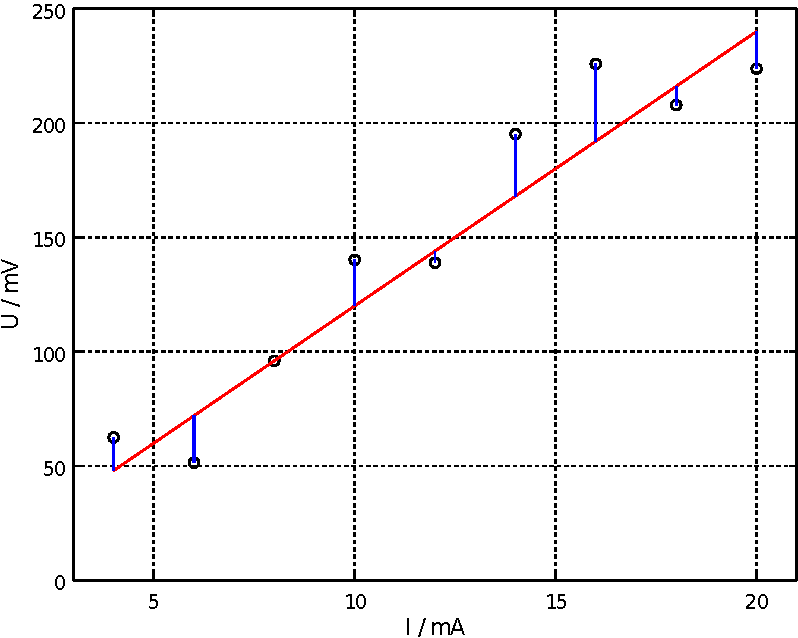
\includegraphics[width=80mm]{01_vorlesung/media/learn_estimation_ohm.pdf}
\caption{Regressionbeispiel: Modellparameter finden, dessen Wert am besten zu den Daten passt}
\label{Ohm1}
\end{center}
\end{figure}

Ob die Spannungswerte zu dem Modell \glqq passen\grqq ~wird bewertet, wobei das Modell
besagt, dass die Spannungswerte gleich dem Widerstand, der genau eine konstante Größe sein soll,
multipliziert mit den eingestellten Werten der Stromstärke seien. Das Bewertungskriterium ist
\glqq die Treffer-Wahrscheinlichkeit Spannungswert liegt auf Widerstand mal Strom\grqq.
Wir gehen davon aus, dass die Abweichungen $\varepsilon_i \; = \; U_i \, - \, R I_i$ normalverteilt sind, also
\begin{equation}
p(U_i,I_i | R) \; \propto \; e^{-\frac{1}{2} \left(\frac{\varepsilon_i}{\sigma_\varepsilon}\right)^2}
\end{equation}
wobei $\sigma_\varepsilon$ ein Maß für die Streuung der Residuen, hier in Millivolt, ist.
Wir haben die Werte der Abweichungen $\varepsilon_i$. Man nennt sie \textbf{Residuen}.
Das Produkt aller Wahrscheinlichkeiten $p(U_i,I_i | R)$ heißt \textbf{Likelihood}.
\begin{equation}
L((U_1,\dots, U_J), (I_1,\dots,I_J) | R) \; = \; \prod\limits_{i = 1}^J \, p(U_i,I_i | R)
\end{equation}
Unsere Modellparameter bzw.\ der Modellparameter, die bzw.\ den wir ermitteln wollen, ist $R$ und
für die Streuung der Werte des Parameters $R$ verwenden wir das Formelzeichen $\sigma_R$.

In der frequentistischen Statistik wird von der Vorstellung ausgegangen, dass es einen wahren Wert für
$R$ gibt, dem man sich nähert, je mehr und genauer man misst, der aber wegen der Streuung
der Spannungswerte $U$ nur annähernd bestimmbar ist. Wenn wir die Präzisionsstromquelle unverändert
auf einen festen Wert einstellen und nicht durchfahren und dann mehrfach die Spannungen ablesen, so
beobachten wir dennoch leicht unterschiedliche Werte für die Spannung. Dies ist der Grund dafür
dass die Wertepaare bei durchgefahrenem Strom $(I_j, U_j)$ nicht exakt auf einer Geraden liegen.

Am besten passt das ganze für einen Wert für $R$,
für den $L((U_1,\dots, U_J), (I_1,\dots,I_J) | R)$ maximal wird.
Die Zielfunktion unseres Optimierungsvorgangs ist also:
\begin{equation}
\max_{R} \; L((U_1,\dots, U_J), (I_1,\dots,I_J) | R)
\end{equation}
Solch eine Optimierungsaufgabe heißt \textbf{Maximum-Likelihood}-Verfahren.
\begin{equation}
\max_{R} \; \prod\limits_{i = 1}^J \,  e^{-\frac{1}{2} \left(\frac{\varepsilon_i}{\sigma_\varepsilon}\right)^2}
\label{MaxiLikeR1}
\end{equation}
d.h.\ nach den Gesetzen der Potenzrechnung
\begin{equation}
\max_{R} \; e^{-\frac{1}{2} \sum\limits_{i = 1}^J \, \left(\frac{\varepsilon_i}{\sigma_\varepsilon}\right)^2} .
\label{MaxiLikeR2}
\end{equation}
Das Maximum der Gaußfunktion liegt an der Stelle, an der der Exponent minimal wird.
Wir maximieren die Likelihood, wenn wir ihren Logarithmus minimieren:
\begin{equation}
\min_{R} \; \sum_{i = 1}^J \, \left(\frac{\varepsilon_i}{\sigma_\varepsilon}\right)^2
\label{MaxiLikeLSQ}
\end{equation}
dazu suchen wir die Nullstelle der Ableitung nach dem Modellparameter.
Auf die Suche des Minimums wird auch mit dem Terminus \textsl{Methode der kleinsten Abweichungsquadrate} oder
\textsl{Least Mean Square Method} Bezug genommen.
Hätten wir nicht nur $R$ sondern viele,
dann würden wir den Gradienten bilden.
\begin{equation}
\frac{\partial}{\partial R} \; \sum_{i = 1}^J \, \left(\frac{\varepsilon_i}{\sigma_\varepsilon}\right)^2 \; = \; 0
\end{equation}
d.i.\ in unserem Beispiel
\begin{equation}
\frac{\partial}{\partial R} \; \sum_{i = 1}^J \, \left(\frac{U_i \, - \, R \, I_i}{\sigma_\varepsilon}\right)^2 \; = \; 0
\end{equation}
Wir multiplizieren mit dem Faktor $\sigma_\varepsilon$
\begin{equation}
\frac{\partial}{\partial R} \; \sum_{i = 1}^J \, \left(U_i \, - \, R \, I_i\right)^2 \; = \; 0
\end{equation}
und führen die Differentiation durch
\begin{equation}
\sum_{i = 1}^J \, 2 \left(U_i \, - \, R \, I_i\right) \, I_i \; = \; 0 .
\end{equation}
Für viele Modellparameter gäbe es entsprechend viele solche Gleichungen mit den jeweiligen Ableitungen, so dass
dann hier ein lineares Gleichungssystem stünde, das zu lösen wäre.
Ein numerisches Verfahren zur Lösung linearer Gleichungssysteme ist das Gauß-Jordan-Eliminationsverfahren.
Nun wir nur diese eine Gleichung haben, können wir einfach nach $R$ auflösen.
\begin{equation}
\sum_{i = 1}^J \, U_i \, I_i \; = \; \sum_{i = 1}^J \, R \, I_i \, I_i
\end{equation}
d.h.
\begin{equation}
 R \; = \; \frac{\sum\limits_{i = 1}^N \, U_i \, I_i}{\sum\limits_{i = 1}^N \,  I_i^2}
\end{equation}
Der ermittelte Wert für $R$ mit den Daten aus der Tabelle ist $12.34~\mathrm{\Omega}$, siehe Abb.~\ref{OhmResult}

\begin{figure}
\begin{center}
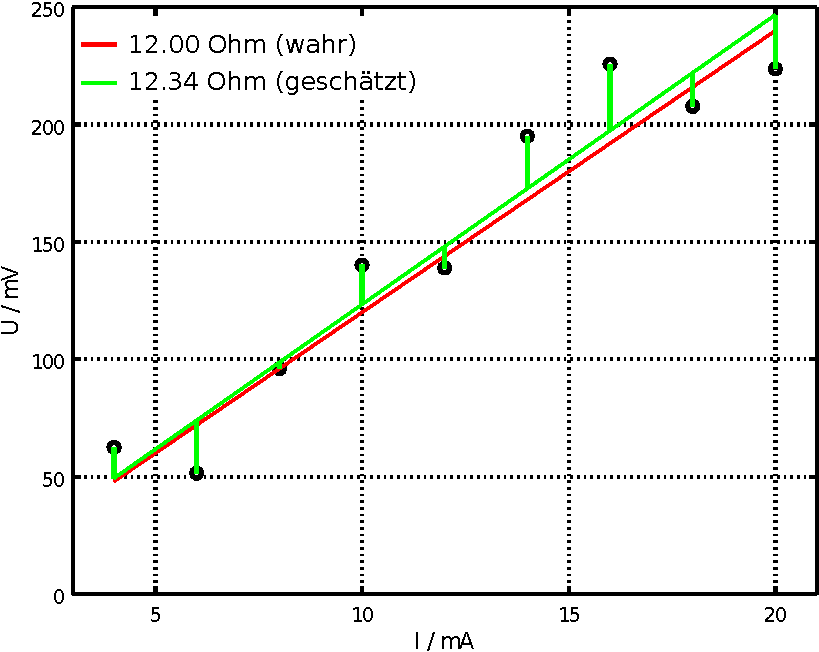
\includegraphics[width=80mm]{01_vorlesung/media/learn_estimation_ohm_esti.pdf}
\label{OhmResult}
\caption{Regressionsbeispiel: Der geschätze Wert des Modellparameters im Vergleich zum wahren.}
\end{center}
\end{figure}

Zuvor haben wir die Likelihood ohne Normierungsfaktor aufgeschrieben.
Eine Wahrscheinlichkeitsdichteverteilung ist so definiert, dass die Fläche unter ihrer Kurve 1 ist, also die Wahrscheinlichkeit
für das Beobachten jedes beliebigen Wertes immer voll eintritt.
\begin{equation}
p(\varepsilon) \; = \; \frac{1}{\sqrt{2 \pi} \sigma_{\varepsilon}} \, e^{-\frac{1}{2} \left(\frac{\varepsilon}{\sigma_{\varepsilon}}\right)^2}
\end{equation}
Ein Maß für die Breite der Gaußglocke ist das $\sigma_{\varepsilon}$ bei etwa 60 Prozent der Höhe ($e^{-\frac{1}{2}} \approx 0.6$).
Ihr Quadrat wird \textbf{Varianz} genannt.
\begin{figure}
\begin{center}
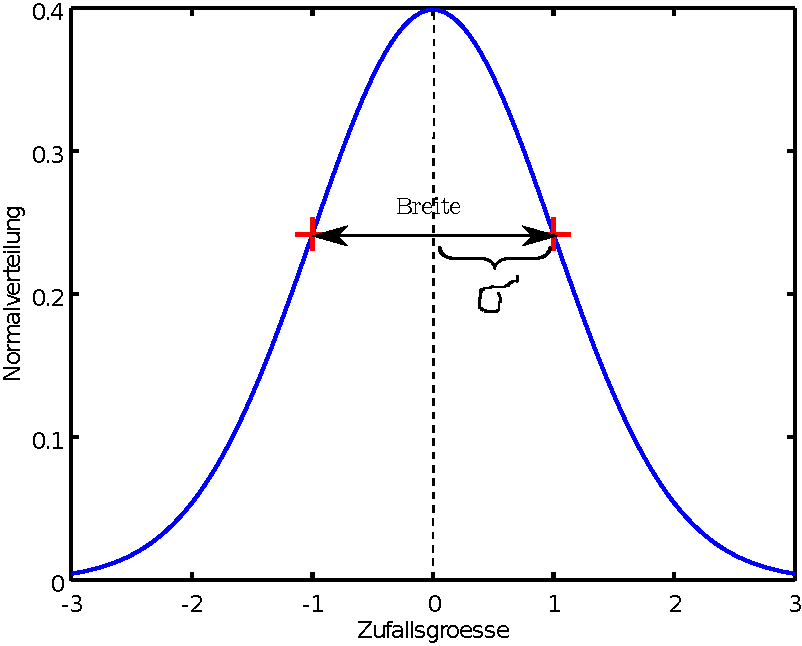
\includegraphics[width=80mm]{01_vorlesung/media/breite_norm_pdf.pdf}
\label{normpdf}
\caption{Breite der Normalverteilung.}
\end{center}
\end{figure}
Das zweite statistische Moment dieser Verteilung 
\begin{equation}
\int_{-\infty}^\infty \, \varepsilon^2 \, p(\varepsilon) \, \mathrm{d} \varepsilon 
\end{equation}
ist gleich dem Quadrat von $\sigma_\varepsilon$, also der Varianz der Gaußverteilung
\begin{equation}
\int_{-\infty}^\infty \, \varepsilon^2 \,  \frac{1}{\sqrt{2 \pi} \sigma_{\varepsilon}} \, e^{-\frac{1}{2} \left(\frac{\varepsilon}{\sigma_\varepsilon}\right)^2} \, \mathrm{d} \varepsilon  \; = \; \sigma_{\varepsilon}^2 .
\end{equation}
Diskretisiert entspricht dies
\begin{equation}
\frac{1}{\sqrt{2 \pi} \sigma_\varepsilon} \, e^{-\frac{1}{2} \left(\frac{\varepsilon}{\sigma_{\varepsilon}}\right)^2} \, \mathrm{d} \varepsilon
\end{equation}
einer relativen Häufigkeit $\frac{n_k}{J-1}$ in der $k$-ten Klasse der Breite $\mathrm{d} \varepsilon$.
Wenn wir nun kein Histogramm mit gleichgroßen Klassenbreiten bilden, sondern zu jedem $\varepsilon_i$ eine Klasse mit der relativen
Häufigkeit $\frac{1}{J-1}$ betrachten, dann haben wir so ungefähr für das $\sigma_{\varepsilon}^2$
\begin{equation}
\sum_{i=1}^J \, \varepsilon_i^2 \,  \frac{1}{J-1}  \; \approx \; \sigma_{\varepsilon}^2 .
\end{equation}
Wir nennen diese Breite wegen der Näherung nicht $\sigma_{\varepsilon}^2$. Diese Näherung ist nur ein ungefährer Schätzwert 
und wird \textbf{empirische Varianz} genannt:
\begin{equation}
s_{\varepsilon}^2 \; = \; \frac{1}{J-1} \, \sum_{i=1}^J \, \varepsilon_i^2
\end{equation}
Wir unterscheiden zwischen der Varianz und der empirischen Varianz durch die Verwendung der
unterschiedlichen Formelzeichen $\sigma$ und $s$.

Uns interessiert aber nicht so sehr die Varianz der Residuen $\varepsilon$, die direkt der Varianz
der Spannungsmessung entspricht,
als viel mehr die Varianz des Modellparameters $R$.
Betrachte die Modellgleichung $R \; = \; \frac{U}{I}$, wie empfindlich reagiert die Größe $R$ auf Veränderung der Größe $U$.
Wählt man anstelle eines Wertes $U$ einen Wert $U \, + \, \Delta U$, so reagiert die Größe $R$ über die Modellgleichung wie folgt
\begin{equation}
R \, + \, \Delta R \; = \; \frac{1}{I} \, \left( U \, + \, \Delta U \right)
\end{equation}
d.i. mit $R \; = \; \frac{U}{I}$
\begin{equation}
\Delta R \; = \; \frac{1}{I} \, \left( \Delta U \right)
\end{equation}
Der Differenzenquotient ist also
\begin{equation}
\frac{\Delta R}{\Delta U} \; = \; \frac{1}{I}
\end{equation}
was bei diesem linearen Zusammenhang direkt hinkommt. Allgemein passt es für stetige Modelle auch bei nichtlinearem Zusammenhang
für genügend kleine Änderungen. Deshalb wird die Empfindlichkeit, die \textbf{Sensitivität}, definiert als die lokale Steigung
\begin{equation}
c  \; = \; \frac{\partial R}{\partial U}
\end{equation}
Die Varianz ist eine quadratische Veränderung, so dass
\begin{equation}
s_R^2  \; = \; \left(\frac{\partial R}{\partial U}\right)^2 \, s_{\varepsilon}^2 \; = \; \frac{1}{I^2} \, s_{\varepsilon}^2
\end{equation}
Hier hätte ich auch direkt $s_R$ aufschreiben können, aber die quadratische Schreibweise wird erforderlich, wenn es um mehrere Größen geht. In den folgenden Vorlesungen werden wir das Konzept der Fortpflanzung der Varianzen kennen lernen.

Die Varianzen sind ein Maß für die Unsicherheit von Messungen. Die \textbf{Messunsicherheit} ist zentrales Thema in der Messtechnik.
Im Wörterbuch der Metrologie (VIM)
\begin{verbatim}
https://www.bipm.org/utils/common/documents/jcgm/JCGM_200_2012.pdf
\end{verbatim}
wird sie wie folgt definiert:
\begin{quote}
\textbf{Messunsicherheit; Unsicherheit} (engl. \textsl{measurement uncertainty; uncertainty}): 
nichtnegativer Parameter, der die Streuung der Werte kennzeichnet, die der Messgröße
auf der Grundlage der benutzten Information beigeordnet ist. [VIM2.26]
\end{quote}
Sie drückt den Mangel einer genauen Kenntnis des Wertes der Messgröße aus.
Selbst wenn systematische Effekte korrigiert werden, bleibt der \textbf{Messwert} lediglich
ein \textbf{Schätz\-wert der Messgröße}, siehe auch GUM:2008, Abschnitt 3.3.1 .

Im Bereich der Metrologie wird zum Thema Messunsicherheitsberechnung eine Richtlinie verwendet,
um die Auswerteverfahren im gesetzlichen Messwesen zu vereinheitlichen und die Resultate
besser vergleichbar zu machen. Die Richtlinie wurde von der
\textsl{Working Group} 1 des \textsl{Joint Committee for Guides in Metrology} (JCGM/WG 1)
entwickelt. Sie hat den Titel \textsl{Evaluation of measurement
data - Guide to the expression of uncertainty in measurement} und wird mit GUM abgekürzt.
Die derzeit gültige Version ist
\textsl{JCGM 100:2008 GUM 1995 with minor corrections} und ist in englischer Fassung
auf der Webseite des \textsl{Bureau international des poids et mesures} (BIPM)
unter folgendem Link frei erhältlich:
\begin{verbatim}
https://www.bipm.org/utils/common/documents/jcgm/JCGM_100_2008_E.pdf
\end{verbatim}

In vielen Fällen reicht es, die Varianzen der einzelnen direkten Messgrößen zu untersuchen sowie
den Zusammenhang zwischen der Variation einer direkten Messgröße und die dadurch verusachte
Veränderung der indirekten, also die Empfindlichkeit/Sensitivität.
Dieser Zusammenhang ist zentrales Thema der Bestimmung von Messunsicherheiten
und wird im Laufe dieser Vorlesung eingehend beleuchtet.
Vielfach gibt es nicht nur einen Zusammenhang zwischen einer direkten mit einer indirekten Messgröße,
sondern auch einen Zusammenhang zwischen den direkten Messgrößen untereinander.

In dieser Vorlesungsreihe liegt das Hauptaugenmerk auf linearen Zusammenhängen zwischen Messgrößen.
Für viele Anwendungen greifen lineare Ansätze. Wenn die betrachteten Bereiche der Variation von Größen
genügend klein sind, so lassen sich auch nichtlineare Modelle durch eine Linearisierung in einer gewissen
Umgebung approximieren.

Das Maß für den linearen Zusammenhang wird \textbf{Korrelation} genannt.
Bei der linearen Regression geht es um Modelle mit indirekten Messgrößen,
die als Koeffizienten eines Polynoms auftreten. Um den Grad des Polynoms zu ermitteln, wird untersucht
mit welchem Potenzgesetz ein Paar direkter Messgrößen zu verknüpfen ist (welchen Grad das Polynom hat),
so dass die Korrelation groß ist.


\section{Charakterisierung von linearem Zusammenhang zwischen Größen}


Bei dem Beispiel mit dem Ohm'schen Gesetz hatten wir uns mit der Modellgleichung $U = R I$ befasst.
Dabei waren $U$ und $I$ die beiden physikalischen Größen, die unterschiedliche Werte angenommen haben und
über einen linearen Zusammenhang verknüpft sind. Hier haben wir also eine Gerade, Polynom vom Grad 1.

Für die Charakterisierung \textsl{linearer} Zusammenhänge ist der
\textbf{Korrelationskoeffizient} $\rho$ ein Maß, mit dem quantifiziert wird, wie
stark zwei Größen linear miteinander verknüpft sind.
Der Korrelationskoeffizient ist so definiert, dass er Werte zwischen $-1$ und
$1$ annehmen kann. Gibt es einen direkten linearen Zusammenhang zwischen zwei Zufallsgrößen
$X_1$ und $X_2$, so wird man zu einer Beobachtung der einen Größe mit kleinem Wert
auch einen kleinen Wert bei der anderen Größe beobachten und wenn die eine Größe einen
großen Wert annimmt, so wird die andere auch einen großen Wert annehmen, und
$\rho$ wird in der Nähe von $1$ liegen. Haben zwei Zufallsgrößen einen ebenso
direkten Zusammenhang, aber in umgekehrter Weise, dass zu kleinen Werten von der ersten
Größe große Werte zur zweiten Größe auftreten und umgekehrt, so liegt $\rho$ in der Nähe von $-1$.
In beiden Fällen sagt man, dass die Größen \textbf{korreliert} seien.

Gibt es überhaupt gar keinen Zusammenhang zwischen dem, was an Werten zu der einen Größe beobachtet
wird mit dem, so ist $\rho = 0$ und man sagt: Die beiden Größen seien \textbf{unkorreliert}.

\begin{figure}
	\begin{center}
		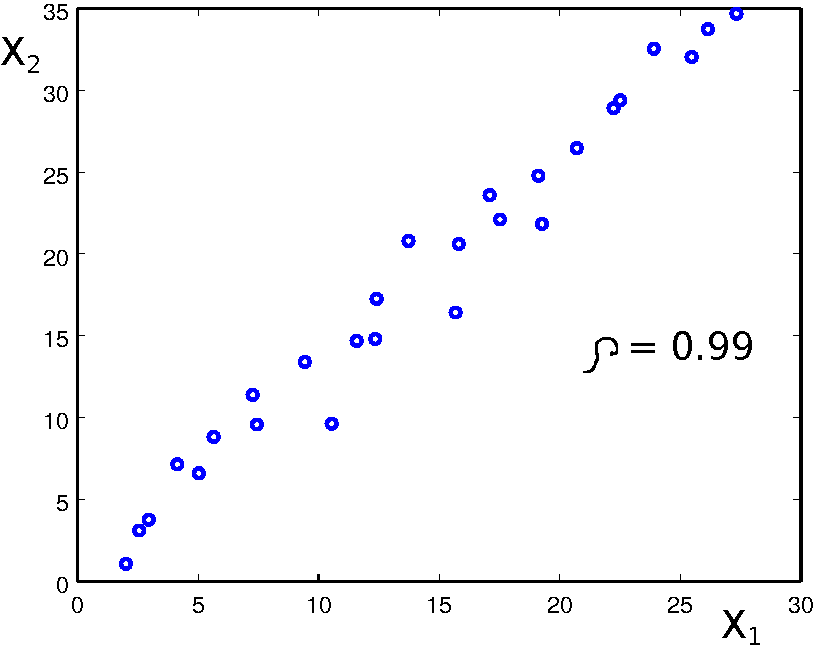
\includegraphics[width=75mm]{01_vorlesung/media/korreliert.pdf} \hspace{5mm}
		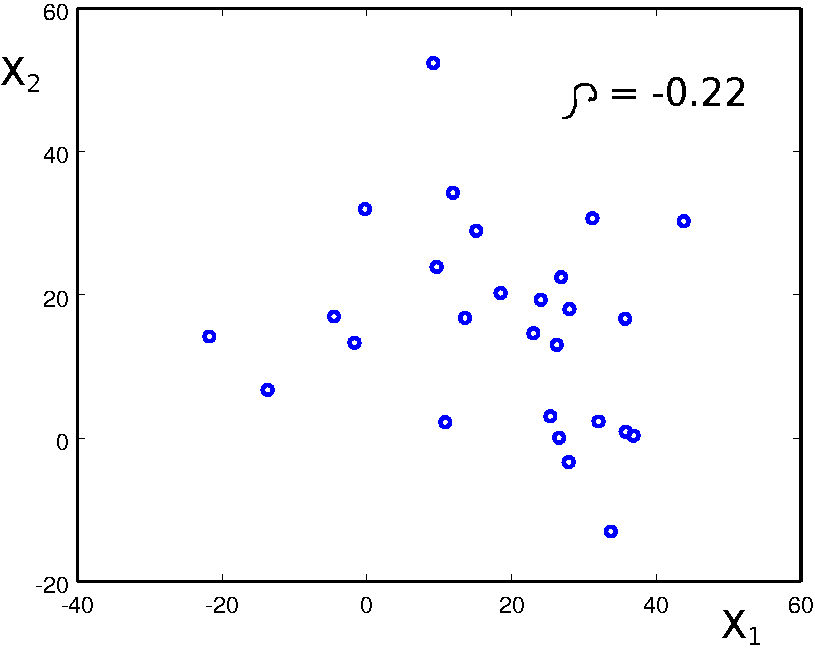
\includegraphics[width=75mm]{01_vorlesung/media/unkorreliert.pdf}
		\caption{\label{korrelation} Wenn es einen linearen Zusammenhang zwischen
			zwei Zufallsgrößen $X_1$ und $X_2$ gibt, so sagt man, dass sie korreliert sind
			und der Korrelationskoeffizient $\rho$ liegt bei Eins (\textsl{links}) oder bei
			minus Eins. Wenn es keinen Zusammenhang zwischen zwei Zufallsgrößen $X_1$ und $X_2$
			gibt, so sagt man, dass sie unkorreliert sind
			und der Korrelationskoeffizient $\rho$ liegt bei Null (\textsl{rechts}).}
	\end{center}
\end{figure}

Die Erwartungswerte zu jeder der Größen $X_1$ und $X_2$ sind jeweils
$\mathrm{E}(X_1)$ und $\mathrm{E}(X_2)$. Sie werden aus den Mittelwerten der jeweiligen
Stichproben geschätzt
\begin{equation}
\bar x_1 \; = \; \frac{1}{J} \, \sum_{j = 1}^J X_{1,j} \qquad
\bar x_2 \; = \; \frac{1}{J} \, \sum_{j = 1}^J X_{2,j}
\end{equation}
Dann ist
\begin{equation}
\mathrm{\bar X} \; = \;
\left(\begin{array}{c}
\bar x_1 \\
\bar x_2
\end{array}
\right)
\end{equation}
der Schwerpunkt der Beobachtungen der Größen.
Sind die Entfernungen der Beobachtungs\-pärchen $(X_{1,j}, X_{2,j})$ vom Schwerpunkt so,
dass die Richtungskomponente der Größe $X_1$ in die gleiche Richtung weist und auch in
proportionale Entfernung wie die Richtungskomponente der Größe $X_2$, so liefern die 
Produkte $(X_{1,j} - \bar x_1)(X_{2,j} - \bar x_2)$ gleiche Vorzeichen. Streuen diese
aber unzusammenhängend, so mitteln sich die unterschiedlichen Terme
$(X_{1,j} - \bar x_1)(X_{2,j} - \bar x_2)$ bei Summation weg.

Wir definieren die Größe
\begin{equation}
s_{1,2} \; := \; \frac{1}{J-1} \, \sum_{j = 1}^J (X_{1,j} - \bar x_1)(X_{2,j} - \bar x_2)
\end{equation}
und nennen sie die \textbf{empirische Kovarianz}.
Allgemein ist die \textbf{Kovarianz} für Zufallsgrößen, deren gemeinsame Verteilung
ihre Wahrscheinlichkeitsdichte $p(X_1, X_2)$ sei, wie folgt definiert
\begin{equation}
\operatorname{Cov}(X_1, X_2) \; := \; 
\int\limits_{-\infty}^{\infty}\int\limits_{-\infty}^{\infty}
(X_1^\prime \, - \operatorname{E}(X_1))(X_2^\prime \, - \operatorname{E}(X_2)) \,
p(X_1^\prime, X_2^\prime) \, \operatorname{d} X_1^\prime \operatorname{d} X_2^\prime .
\end{equation}
Wir sehen hier, dass die Kovarianz einer Zufallsgröße mit sich selbst die
\textbf{Varianz} ist
\begin{equation}
\operatorname{Var}(X_1) \; := \;  \operatorname{Cov}(X_1, X_1) \; = \; 
\int\limits_{-\infty}^{\infty}
(X_1^\prime \, - \operatorname{E}(X_1))^2 \,
p(X_1^\prime) \, \operatorname{d} X_1^\prime
\end{equation}
und für die empirsche Varianz und Kovarianz gilt entsprechend
\begin{equation}
s_{1}^2 \; := \; s_{1,1} \; = \; 
\frac{1}{J-1} \, \sum_{j = 1}^J (X_{1,j} - \bar x_1)^2 .
\end{equation}
Wir werden im nächsten Kapitel sehen, dass bei der Steigung der Regressionsgraden
(Aufgabe 1) genau so ein Term $\sum_{j = 1}^J (X_{1,j} - \bar x_1)(X_{2,j} - \bar x_2)$
im Zähler steht.

Für das Verständnis der Gesamtzusammenhänge ist der Sprachgebrauch für Zufallsgrößen sowie
der Sprachgebrauch des Erwartungswertes von Zufallgrößen von Bedeutung. 

Verknüpfungen von Zufallsgrößen sind ihrerseits wieder Zufallsgrößen. Betrachten
wir eine Größe $X$, die ganz abstrakt und allgemein eine Zufallsgröße ist, und
$p(X)$ die Wahrscheinlichkeitsdichteverteilung dazu, so heißt
\begin{equation}
\operatorname{E}(X) \; := \;  \int\limits_{-\infty}^{\infty}
X^\prime \, p(X^\prime) \, \operatorname{d} X^\prime
\end{equation}
Erwartungswert der Zufallsgröße $X$.
Ist diese Zufallsgröße eine Verknüpfung von anderen Zufallsgrößen und setzen wir die
Verknüpfung ein, so wird der Erwartungwert mit derselben Verknüpfung gebildet.
Betrachten wir zum Beispiel die Verknüpfung Addition $X = X_1 + X_2$
\begin{equation}
\operatorname{E}(X_1 + X_2) \; := \;  \int\limits_{-\infty}^{\infty} \int\limits_{-\infty}^{\infty}
(X_1^\prime + X_2^\prime) \, p(X_1^\prime, X_2^\prime) \, \operatorname{d} X_1^\prime \, \operatorname{d} X_2^\prime
\end{equation}
d.h.
\begin{equation}
\arraycolsep=2.0pt\def\arraystretch{2.0}
\begin{array}{ll}
\operatorname{E}(X_1 + X_2) \; = & \int\limits_{-\infty}^{\infty} \int\limits_{-\infty}^{\infty}
X_1^\prime \, p(X_1^\prime, X_2^\prime) \, 
\operatorname{d} X_1^\prime \, \operatorname{d} X_2^\prime\\
& + \; \int\limits_{-\infty}^{\infty} \int\limits_{-\infty}^{\infty} 
X_2^\prime \, p(X_1^\prime, X_2^\prime) \, \operatorname{d} X_1^\prime \, \operatorname{d} X_2^\prime
\end{array}
\end{equation}
und mit der Randverteilung (engl.\ \textsl{marginal distribution}) 
\begin{equation}
p(X_2) \; = \;
\int\limits_{-\infty}^{\infty} p(X_1^\prime, X_2) \, \operatorname{d} X_1^\prime
\label{marginalDistr}
\end{equation}
erhalten wir
\begin{equation}
\operatorname{E}(X_1 + X_2) \; = \; \int\limits_{-\infty}^{\infty}
X_1^\prime \, p(X_1^\prime) \, \operatorname{d} X_1^\prime 
\; + \; \int\limits_{-\infty}^{\infty} 
X_2^\prime \, p(X_2^\prime) \, \operatorname{d} X_2^\prime
\end{equation}
also
\begin{equation}
\operatorname{E}(X_1 + X_2) \; = \; \operatorname{E}(X_1) \; + \; \operatorname{E}(X_2).
\label{EwSummeISTSummeEw}
\end{equation}
In Worten heißt dies: Der Erwartungswert einer Summe von Zufallsgrößen ist die
Summe der Erwartungswerte der Zufallsgrößen.

Als nächstes betrachten wir das Produkt zweier Zufallsgrößen
$X = X_1 \cdot X_2$
\begin{equation}
\operatorname{E}(X_1 \cdot X_2) \; := \; 
\int\limits_{-\infty}^{\infty} \int\limits_{-\infty}^{\infty}
X_1^\prime \, X_2^\prime \; p(X_1^\prime, X_2^\prime) \,
\operatorname{d} X_2^\prime\, \operatorname{d} X_1^\prime .
\end{equation}
Die Kovarianz ist der Erwartungswert folgenden Produktes
$(X_1 - \operatorname{E}(X_1)) \cdot (X_2 - \operatorname{E}(X_2))$
\begin{equation}
\operatorname{E}((X_1 - \operatorname{E}(X_1)) \cdot
(X_2 - \operatorname{E}(X_2))) \; = \; 
\int\limits_{-\infty}^{\infty} \int\limits_{-\infty}^{\infty}
(X_1^\prime - \operatorname{E}(X_1)) \cdot (X_2^\prime - \operatorname{E}(X_2))
\, p(X_1^\prime, X_2^\prime) \, 
\operatorname{d} X_1^\prime\, \operatorname{d} X_2^\prime
\end{equation}
also
\begin{equation}
\operatorname{Cov}(X_1, X_2)  \; = \; \operatorname{E}\left((X_1 - \operatorname{E}(X_1)) 
\cdot (X_2 - E(X_2)) \right)  .
\end{equation}
Ferner ist zu bemerken, dass sich aus diesen Beziehungen für die
Kovarianz ergibt
\begin{equation}
\begin{array}{ll}
\operatorname{Cov}(X_1, X_2)
& \; = \;  \operatorname{E}\left(X_1 \, X_2 - X_2 \, \operatorname{E}(X_1) -
X_1 \, \operatorname{E}(X_2) + \operatorname{E}(X_1) \, \operatorname{E}(X_2) \right) \\
& \; = \;  \operatorname{E}(X_1 \, X_2)  - \operatorname{E}(X_2) \, \operatorname{E}(X_1)
- \operatorname{E}(X_1) \, \operatorname{E}(X_2) + \operatorname{E}(X_1) \, \operatorname{E}(X_2)) \\
& \; = \;  \operatorname{E}(X_1 \, X_2) - \operatorname{E}(X_1) \, \operatorname{E}(X_2) .
\end{array}
\label{ErwartungsCOV}
\end{equation}
Per Definitionem gilt
\begin{equation}
\operatorname {Var}(X) \; := \; \operatorname {Cov}(X,X) .
\end{equation}
Daraus folgt, dass für die Varianz einer Zufallsgröße,
die das Produkt einer Zufallsgröße $X$ mit einem konstanten, festen reellen Faktor $b$ ist, gilt
\begin{equation}
\operatorname {Var}(b X) \; := \; b^2 \, \operatorname {Var}(X)
\end{equation}
%Für einen Zufallsgrößenvektor $\boldsymbol{X}$ multipliziert mit einer Matrix 
%$\boldsymbol{B}$, deren Elemente konstante, feste reelle Zahlen sind, gilt entsprechend
%\begin{equation}
%\operatorname {Cov}(\boldsymbol{B} \boldsymbol{X}) \; := \; \boldsymbol{B} \,
% \operatorname {Cov}(\boldsymbol{X}) \, \boldsymbol{B}^\mathsf{T} .
%\label{CovarianzKonstMatrix}
%\end{equation}
%Das ist jetzt nicht trivial herzuleiten, aber wir wollen jetzt keine Vorlesung in Lineare
%Algebra halten. Wir werden diese Beziehung für die Bestimmung der Standardabweichung der
%Modellparameter in der linearen Regression brauchen. Das hochgestellte $\mathsf{T}$ steht für
%transponiert.

Eine weitere wichtige Beziehung ist folgende zur
\textbf{Varianz einer Summe von Zufallsgrößen}:
\begin{equation}
\operatorname {Var}\left(\sum _{{i=1}}^{N}X_{i}\right) \; = \;
\sum _{{i,j=1}}^{N}\operatorname {Cov}(X_{i},X_{j})
\label{VarianzSummeISTSummeKovarianz}
\end{equation}
Die Varianz ist nach Definition
\begin{equation}
\operatorname {Var}\left(\sum _{{i=1}}^{N}X_{i}\right) \; = \;
\int\limits_{-\infty}^{\infty} \dots \int\limits_{-\infty}^{\infty}
\, \left[ \left(\sum_{i=1}^N X_i\right) \; - \; E(\sum_{i=1}^N X_i) \right]^2 \, p(X_1, \dots, X_2)
\, \operatorname{d}X_1 \dots \operatorname{d}X_N .
\end{equation}
Da der Erwartungswert einer Summe von Zufallsgrößen gleich der Summe der 
Erwartungswerte jeder einzelnen dieser Zufallsgrößen ist, siehe Gl.~(\ref{EwSummeISTSummeEw}), gilt
$$
\left(\sum_{i=1}^N X_i \right) \; - \; E(\sum_{i=1}^N X_i) \; = \;
\left(\sum_{i=1}^N X_i \right) \; - \; \sum_{i=1}^N E(X_i) 
$$
so dass gilt
\begin{equation}
\operatorname {Var}\left(\sum _{{i=1}}^{N}X_{i}\right) \; = \;
\int\limits_{-\infty}^{\infty} \dots \int\limits_{-\infty}^{\infty}
\, \left[ \sum_{i=1}^N \left(X_i \; - \; E(X_i)\right) \right]^2 \, p(X_1, \dots, X_2)
\, \operatorname{d}X_1 \dots \operatorname{d}X_N .
\end{equation}
Mit Anwendung des Assoziativgesetzes
$$
\arraycolsep=3.5pt\def\arraystretch{1.8}
\begin{array}{ll}
\left[ \sum\limits_{i=1}^N \left(X_i \; - \; E(X_i)\right) \right]^2 & =
\left[ \sum\limits_{i=1}^N \left(X_i \; - \; E(X_i)\right) \right] \;
\left[ \sum\limits_{k=1}^N \left(X_k \; - \; E(X_k)\right) \right] \\
& = \sum\limits_{i=1}^N \sum\limits_{k=1}^N  \left(X_i \; - \; E(X_i)\right) \;
\left(X_k \; - \; E(X_k)\right) \\
\end{array}
$$
gilt
\begin{equation}
\operatorname {Var}\left(\sum _{{i=1}}^{N}X_{i}\right) \; = \;
\int\limits_{-\infty}^{\infty} \dots \int\limits_{-\infty}^{\infty}
\, \sum_{i=1}^N \sum_{k=1}^N  \left(X_i \; - \; E(X_i)\right) \;
\left(X_k \; - \; E(X_k)\right) \, p(X_1, \dots, X_2)
\, \operatorname{d}X_1 \dots \operatorname{d}X_N .
\end{equation}
Durch Berechnung der Marginalverteilungen und weil $\int p(X_j) \, \operatorname{d}X_j = 1$
für alle $j$, die weder $i$ noch $k$ sind, erhalten wir
\begin{equation}
\operatorname {Var}\left(\sum _{{i=1}}^{N}X_{i}\right) \; = \;
\sum_{i=1}^N \sum_{k=1}^N  \;
\int\limits_{-\infty}^{\infty} \int\limits_{-\infty}^{\infty}
\, \left(X_i \; - \; E(X_i)\right) \;
\left(X_k \; - \; E(X_k)\right) \, p(X_i, X_k)
\, \operatorname{d}X_i \operatorname{d}X_k .
\end{equation}
Der Term auf der rechten Seite ist genau die Kovarianz der beiden 
Größen $X_i$ und $X_k$.

Die Beziehung Gl.~(\ref{VarianzSummeISTSummeKovarianz}), dass die
Varianz der Summe von Zufallsgrößen gleich der Summe der paarweisen Kovarianzen
ist, werden wir im Laufe dieser Vorlesungsreihe häufig
verwenden:
\begin{equation}
{\begin{aligned}\operatorname {Var}\left(\sum _{{i=1}}^{N}X_{i}\right) & 
	= \sum _{i=1}^{N}\sum _{k=1}^{N}\operatorname {Cov}(X_{i},X_{k})\\
	& = \sum _{{i=1}}^{N}\operatorname {Var}(X_{i})+
	\sum _{{i,k=1,i\neq k}}^{N}\operatorname {Cov}(X_{i},X_{k})\\
	& = \sum _{i=1}^{N}\operatorname {Var}(X_{i})+2\sum _{{i=1}}^{{N-1}}
	\sum _{k=i+1}^{N}\operatorname {Cov}(X_{i},X_{k}) ,
	\end{aligned}}
\label{VarianzSummeX2Kovarianz}
\end{equation}
Dies lässt sich für den Fall erweitern, dass die summierten Zufallsgrößen mit jeweils einem reellen,
konstanten Faktor multipliziert werden:
\begin{equation}
{\begin{aligned}\operatorname {Var}\left(\sum _{{i=1}}^{N} \, c_i \, X_{i}\right) & 
	= \sum _{i=1}^{N}\sum _{k=1}^{N}\operatorname {Cov}(c_i X_{i}, c_k X_{k})\\
	& = \sum _{{i=1}}^{N} \, c_i^2 \, \operatorname {Var}(X_{i})+
	\sum _{{i,k=1,i\neq k}}^{N} \, c_i c_k \,  \operatorname {Cov}(X_{i},X_{k})\\
	& = \sum _{{i=1}}^{N} \, c_i^2 \operatorname {Var}(X_{i})+2\sum _{{i=1}}^{{N-1}}
	\sum _{{k=i+1}}^{N} \, c_i c_k \operatorname {Cov}(X_{i},X_{k}).
	\end{aligned}}
\label{KovarianzSumme}
\end{equation}
Auf Gleichung (\ref{KovarianzSumme}) werden wir in den nächsten Vorlesungen zurück kommen,
denn diese ist die Grundlage für das \textbf{Gesetz zur Fortpflanzung von Messunsicherheiten}.

Für standardnormalverteilte Zufallsgrößen $Z_i$ mit $Z \sim \mathcal{N}(0,1)$ 
und $i = 1,2$ in die sich
die Größen $X_i$ wie folgt umrechnen lassen
\begin{equation}
Z_i \; = \; \frac{X_i \, - \, \operatorname{E}(X_i)}{\sqrt{\operatorname {Var}(X_{i})}}
\end{equation}
ist die Kovarianz gleich dem Korrelationskoeffizienten
\begin{equation}
\rho_{i,k} \; = \; \operatorname {Cov}(Z_{i},Z_{k})
\end{equation}
was äquivalent ist zu
\begin{equation}
\rho_{i,k} \; = \; \frac{\operatorname {Cov}(X_{i},X_{k})}{\sqrt{\operatorname {Var}(X_{i})} \, \sqrt{\operatorname {Var}(X_{k})}} .
\end{equation}


\section{Beispiel zum Selbststudium}
Zu Bestimmen ist ein Ohmscher Widerstand $R$ sowie eine Offsetspannung $U_0$ bei gegebenen Werten einer
Präzisionsstromquelle und eines Voltmeters:

\begin{center}
\begin{tabular}{l||c|c|c|c|c|c|c|c|c}
\hline\hline
 $I$ in mA &    4.0 &     6.0 &     8.0 &    10.0 &    12.0 &    14.0 &    16.0 &    18.0 &    20.0\\
\hline
 $U$ in mV &    62.5 &    51.5 &    96.0 &   140.2 &   138.9 &   195.1 &   225.8 &   207.8 &   223.7 \\
\hline\hline
\end{tabular}
\end{center}

Es wird angenommen, dass die Stromstärken ohne Streuung vorliegen (als Regressoren) und die Spannungen normalverteilt
streuen (als Regressanden), so dass
\begin{equation}
\min_{R, U_0} \; \sum_{i = 1}^J \, \left(U_i \, - \, R \, I_i  \, - \,  U_0\right)^2
\label{regrGer}
\end{equation}

\begin{itemize}
\item[(a)] Berechnen Sie den Korrelationskoeffizienten $\rho(I, U)$
\item[(b)] Lösen Sie das Gleichungssystem
\begin{equation}
\left(\begin{array}{c}
\frac{\partial}{\partial R}\\
\frac{\partial}{\partial U_0}
\end{array}\right)
\, \sum_{i = 1}^J \, \left(U_i \, - \, R \, I_i  \, - \,  U_0\right)^2 \; = \;
\left(\begin{array}{c}
0\\
0
\end{array}\right)
\label{regrGerGS}
\end{equation}
\item[(c)] Berechnen Sie die aus der Lösung des Gleichungssystems aus (a) gewonnen Schätzwerte
für $R$ und $U_0$.
\end{itemize}




%
\chapter{Lineare Regression (Ausgleichsrechnung)}
\label{KapitellinReg}

\section{Die Idee der linearen Regression}
\label{RegressionsIdee}

Ziel der Regression ist es, den funktionalen Zusammenhang $Y =
f(X_{1} ,X_{2} ,...,X_{N} )$ zwischen den
Eingangs-Messgrößen $X_{i}$ (Regressor) und der Ausgangsgröße $Y$
(Regressanden) möglichst gut zu charakterisieren.

Der allgemeinste Fall der Regressionsrechnung ist der mit sowohl mehreren
Regressoren als auch mehreren Regressanden.
Regressionsrechnung mit einem Regressanden, wird \textbf{univariate Regression}, oder oft einfach nur lineare Regression genannt.
Die Darstellung der Modellgleichung kann dabei wie folgt aussehen 
\begin{equation}
Y_j = f(X_{1,j},\dots, X_{i,j},\dots, X_{N,j}) + \varepsilon_j \quad \mathrm{mit} \quad j = 1,2,\ldots,J
\label{Kap2Modellglunivar}
\end{equation}
wobei $Y_j$ eine Beobachtung zur Zufallsgröße, dem Regressanden $Y$, darstellt bei Vorgabe (Einstellung an einem
Gerät wie im Beispiel von Kapitel 1 der Präzisionsstromquelle) $X_{i,j}$ des Regressors $X_i$.
Wenn es mehrere abhängige Größen, also mehrere Regressanden gibt, spricht man von \textbf{multivariater Regression}. Die Regressoren müssen voneinander \textbf{linear unabhängig} sein.

Sie können aber auch eine Potenzbeziehung zueinander haben, also quadratisch, kubisch etc.
Wir werden für die Methode der Regressionsrechnung zur Schätzung von Polynomkoeffizienten
eine Eingangsgröße $X$ und eine Ausgangsgröße $Y$ betrachten, die über ein Potenzgesetz
\begin{equation}
Y = f(X) \propto X^k \quad \mathrm{mit} \quad k \in I \! \! N_0
\label{potenzgesetzlinReg}
\end{equation}
also mit $k$ als natürliche Zahl einschließlich der Null, verknüpft sind.

Bei der Regressionsrechnung wird vorausgesetzt,
dass der Regressor $X$ eine Größe ist, die voreingestellt ist und keiner Streuung unterliegt,
und nur der Regressand $Y$ streut und deshalb als Zufallsgröße betrachtet wird.
Die Streuung kann verschiedene Ursachen haben:
\begin{itemize}
\item Die indirekten Messgrößen, hier die Größen, die durch die
Modellparameter beschrieben werden, streuen aufgrund von nicht im Modell
enthaltenden Einflüssen.
Das bedeutet, dass das Modell eine Approximation des physikalischen Sachverhalts ist.
\item Der Messvorgang des Regressanden führt zu Streuungen.
\end{itemize}
Die Modellparameter sind also wie die Regressanden als Zufallsvariablen
zu betrachten. Die Regression soll nun Schätzwerte für die
Modellparameter liefern. Das Modell wird über einen 
funktionalen Zusammenhang zwischen Regressor und Regressand 
\begin{equation}
Y = f(X)
\label{Kap2Modellgleichung}
\end{equation}
beschrieben.

Um eine Schätzung für die Parameter des funktionalen Zusammenhangs $Y = f(X)$
zu erhalten, wird die Eingangsgröße in einem bestimmten Bereich
variiert. Man misst $J$ Messwertpaare $(X_j ,Y_j )$ mit $j=1,\ldots, J$, die sich als Punktwolke in einem Diagramm darstellen lassen. Auf Grund der Streuungen werden die Wertepaare $(X_j, Y_j )$
die Gleichung $Y_j = f(X_j )$ nicht exakt erfüllen,
sondern etwas abweichen $\varepsilon_j$, d.~h.
\begin{equation}
Y_j = f(X_j) + \varepsilon_j \quad \mathrm{mit} \quad j = 1,2,\ldots,J
\label{Kap2ModellglmitResiduen}
\end{equation}

Wir stellen hier zusammen welche Typen von Größen bei der Regressionsrechnung behandelt werden:
\begin{itemize}
	\item Die unabhängigen Größen $X$ werden
	 vorgegeben. Sie haben genau bekannte Werte (engl.\ \textsl{exactly known values})
	und sind somit keine Zufallsgrößen. Sie sind unabhängig und 
	heißen \textbf{Regressoren}.
	\item Die abhängigen Größen $Y$, d.h.\ die \textbf{Regressanden} streuen und ihre Residuen sind
	normalverteilt mit Erwartungswert $E(\varepsilon) = 0$ und Varianz $\mathrm{Var}(\varepsilon) = \sigma^2$. 
	
	Die Residuen sind \textbf{unabhängig und identisch verteilt}, kurz u.i.v.
	\begin{equation}
	\varepsilon \; \overset{u.i.v.}{\sim} \; \mathcal{N}(0,\sigma_{\varepsilon}) .
	\label{Resinormalverteilt}
	\end{equation}
	Die Regressanden werden auf Grund ihrer Streuung als Zufallsgrößen betrachtet.
	Zu jedem beobachteten Wert des Regressanden wird jeweils ein Regressorwert
	zugeordnet (engl. \textsl{observed data corresponding to the known values}).
	Sie sind abhängig vom Regressor und werden deshalb auch \textsl{dependent variable} oder
	\textsl{response variable} genannt.
	\item Modellparameter, die unbekannt sind (\textsl{unknown parameters}), sind Zufallsgößen. Sie werden
	auch Regressionsparameter (\textsl{regression parameters}) genannt.
	\item Ferner gibt es zusätzliche unbekannte Parameter, und zwar die Varianzen der beteiligten
	Zufallsgrößen, \textsl{unknown additional parameters}. % $\boldsymbol{\delta}$ (unknown variance parameters)
\end{itemize}
	
\begin{figure}
	\begin{center}
		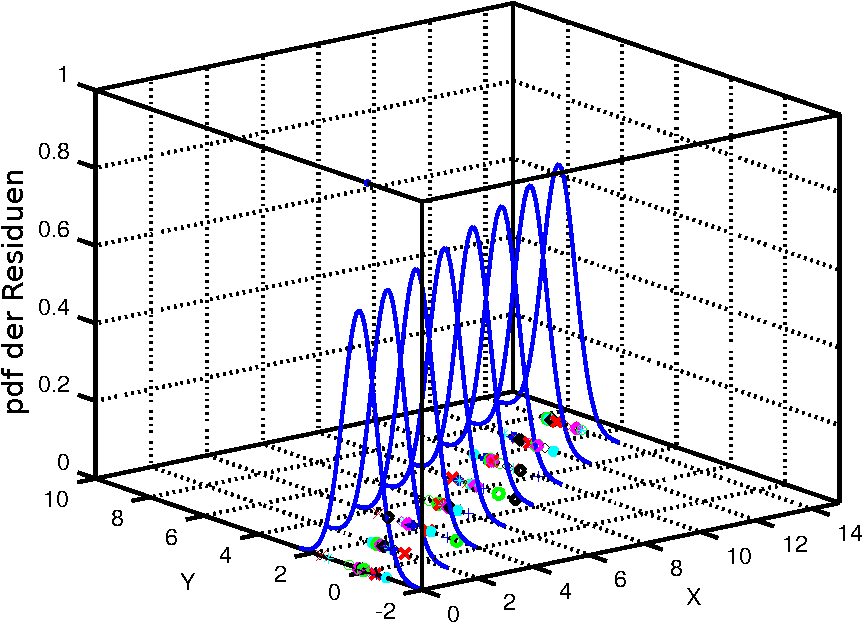
\includegraphics[width=100mm]{02_vorlesung/media/regressionNormalResi_1b.pdf}
		\caption{\label{regressionNormalResi} Lineare Regression für unabhängig und
			identisch verteilte Residuen.}
	\end{center}
\end{figure}

Abb.~\ref{regressionNormalResi} veranschaulicht, dass die Residuen normalverteilt sind, wobei die vertikale Achse die Wahrscheinlichkeitsdichte der Residuen darstellt. Der englische Begriff für Wahr\-schein\-lich\-keits\-dichte\-ver\-teil\-ung ist \textsl{probability density function}, kurz pdf. Die unterschiedlichen
Farben und Symbole sollen unterschiedliche Durchläufe gleicher Messvorgänge darstellen.

\section{Lineare Regression als Beispiel zur Methode der kleinsten Abweichungsquadrate}

Man bestimmt die Parameter der Regressionsfunktion $Y =
f(X)$ nun so, dass die Summe der Quadrate der
Abweichungen der Datenpunkte vom Modell (\textbf{Residuen}) $\varepsilon_j $ möglichst klein wird
(Methode der kleinsten Abweichungsquadrate),
d.h.\ die \textbf{Kostenfunktion} $Q$ muss minimal werden:
\begin{equation}
Q: = \sum\limits_{j = 1}^J {\varepsilon_j ^2 = } \sum\limits_{j = 1}^J {(Y_j
	- f(X_j ))^2 \to } \,\,\min
\label{eq:Minimimierung-kleinster-Fehlerquadrate}
\end{equation}
Die Kostenfunktion ist ein Maß für die Abweichung der Messgrößen vom Modell in Abhängigkeit von der
Wahl der Werte für die Modellparameter. Für gegebene Werte für die Modellparameter liefert die
Kostenfunktion ein Maß für die Qualtität der Schätzung und wird \textbf{Qualitätsmaß} genannt.

Wie in Kapitel 1 dargelegt, basiert dies auf dem Maximieren der Likelihood, der
normalverteilten bzw.\ gaußverteilten Wahrscheinlichkeitsdichte der Residuen. Da diesem Verfahren
die Annahme als Voraussetzung zugrunde liegt, dass die Likelihood gaußverteilt ist, spricht man in der
ingenieurmäßigen Anwendung auch vom Ausgleichsverfahren nach Gauß.

In die Modellgleichung (\ref{Kap2Modellgleichung}) setzen wir mehrere Potenzgesetze (\ref{potenzgesetzlinReg})
ein, um folgenden Polynomansatz aufzustellen
\begin{equation}
Y = f(X) \equiv p_m = \theta _m X ^m + \theta _{m-1} X^{m - 1} + 
\cdots + \theta _1 X + \theta _0
\end{equation}
$m$ bezeichnet den Grad des Polynoms. Die Anzahl der Regressionsparameter bezeichnen wir mit $M = m+1$.
Unter Berücksichtigung der Streuung der Beobachtungen $Y_j$ des Regressanden ist dies wie in Gl.~(\ref{Kap2ModellglmitResiduen})
\begin{equation}
Y_j = f(X_j) \equiv p_m = \theta _m X_j^m + \theta _{m-1} X^{m - 1} + \cdots + 
\theta _1 X_j + \theta _0 + \varepsilon_j
\end{equation}

Für die Schätzung der Polynomkoeffizienten setzen wir den Polynomansatz in die 
Minimumbedingung Gl.~(\ref{eq:Minimimierung-kleinster-Fehlerquadrate}) ein:
\begin{equation}
Q = Q(\theta _m ,\theta _{m - 1} ,\ldots ,\theta _1 ,\theta _0 ) =
\sum\limits_{j = 1}^J {(Y_j - p_m (X_j ))^2 \to } \,\,\min
\end{equation}

Die Schätzwerte der Koeffizienten $\hat{\theta}_k$, für die die Kostenfunktion $Q$ ein Minimum annimmt, sind
die beste Schätzung oder das Optimum der Parameter $\theta _k $, weshalb im englischen Sprachgebrauch auch der Begriff
\textsl{best fit} Verwendung findet. Die optimalen Schätzwerte zu den
Polynomkoeffizienten $\hat{\theta}_k$ ergeben sich durch Lösen des linearen Gleichungssystems,
das sich durch Null setzten der partiellen Ableitungen von $Q$ nach den Modellparametern ergibt:
\begin{equation}
\left. {\frac{\partial Q}{\partial \theta _k }} \right|_{\theta_k
	=  \hat\theta_k } = 0,\,\,k = 0,1,\ldots ,m
\label{linRegGleichungssystem}
\end{equation}
Die resultierende Modellgleichung ist dann die mit den geschätzten
Regressionsparametern (hier den Polynomkoeffizienten) $\hat\theta_k$:
\begin{equation}
Y = f(X) \equiv p_m = \hat\theta_m X ^m + \hat\theta_{m - 1} X
^{m - 1} + \cdots \hat\theta_1 X + \hat\theta_0
\end{equation}
Ein Schätzwert für die Varianz der Residuen, d.h.
$\mathrm{Var}(\varepsilon)$, ergibt sich durch die empirische Varianz:
\begin{equation}
\mathrm{Var}(\varepsilon(\hat{\theta}_m ,\hat{\theta}_{m - 1} ,\ldots ,\hat{\theta}_1 
,\hat{\theta_0} )) = s^2 = \frac{Q(\hat{\theta}_m ,\hat{\theta}_{m - 1}
	,\ldots ,\hat{\theta}_1 ,\hat{\theta_0} )}{J - 1 - m}
\label{eq:s_quadrat_Regresssion}
\end{equation}


Wir betrachten zunächst den einfacheren Fall der \textbf{linearen Regression},
bei dem eine empirische Regressionsgerade  gesucht wird, d.~h. 
es gibt nur zwei Modellparameter $\theta_0$ und $\theta_1$:
\begin{equation}
Y = \theta_0 + \theta_1 \cdot X
\end{equation}
Die beste Schätzung für die Parameter $\theta _0 $und
$\theta _1 $ findet man durch Minimierung gemäß
Gl.~(\ref{eq:Minimimierung-kleinster-Fehlerquadrate}),
d.~h.
\begin{equation}
\label{eq:linRegrMinimierung}
Q(\theta _0 ,\theta _1 ) = \sum\limits_{j = 1}^J {(Y_j
	- (\theta _0 + \theta _1 \cdot X_j))^2 \to } \,\,\min
\end{equation}

Für jedes vorgegebene Messwertpaar-Ensemble $(X_j ,Y_j )$, $j
= 1,2,\ldots J$ existiert eine eindeutige Lösung der Gl.
(\ref{eq:linRegrMinimierung}).

Zum Auffinden des Minimums der Gl.(\ref{eq:linRegrMinimierung}), bildet man die
partiellen Ableitungen und setzt diese gleich Null:
\begin{equation}
\renewcommand*{\arraystretch}{1.5}
\begin{array}{lcc}
\left. {\frac{\partial Q(\theta _0 ,\theta _1 )}{\partial \theta_0 }} 
\right|_{\theta _0 = \hat{\theta}_0 ,\,\theta _1 = \hat{\theta}_1 } & = & 0  \\
\left. {\frac{\partial Q(\theta _0 ,\theta _1 )}{\partial \theta_1 }} 
\right|_{\theta _0 = \hat{\theta}_0 ,\,\theta _1 = \hat{\theta}_1 } & = & 0 
\end{array}
\label{GleichungssytemKostenfkt}
\end{equation}
Für das Vorliegen eines Minimums (nicht Maximum oder Sattelpunktes) müssen noch 
die Bedingungen
\begin{equation}
	\left. {\frac{\partial^2 Q(\theta _0 ,\theta _1 )}{\partial \theta_0^2 }} 
\right|_{\theta _0 = \hat{\theta}_0 ,\,\theta _1 = \hat{\theta}_1 } > 0 \quad 
\mathrm{und} \quad \left. { \frac{\partial^2 Q(\theta _0 ,\theta _1)}{ \partial \theta_1^2 }} 
\right|_{\theta _0 = \hat{\theta}_0 ,\,\theta _1 = \hat{\theta}_1 } > 0
\end{equation}
erfüllt sein.

Daraus folgt:
\[
\sum\limits_{j = 1}^J {Y_j - J} \, \hat{\theta}_0 - \hat{\theta}_1 \sum\limits_{j = 1}^J {X_j = 0}
\]
\[
\sum\limits_{j = 1}^J {Y_j X_j - \theta_0 \sum\limits_{j = 1}^J {X_j - \theta_1 \sum\limits_{j = 1}^J {X_j ^2 = 0} } }
\]

Mit $\sum\limits_{j = 1}^J {X_j } = J \, \bar {X}$ und 
$\sum\limits_{j= 1}^J {Y_j } = J \, \bar {Y}$ folgt:
\[
J \, \bar {Y} - J \, \hat{\theta}_0 - J \cdot \hat{\theta}_1 \, \bar {X} = 0 \quad
\mathrm{bzw.}\quad \hat{\theta}_0 = \bar {Y} - \hat{\theta}_1 \, \bar {X}
\]

\[
\sum\limits_{j = 1}^J {X_j \, Y_j \; - \; J \hat{\theta}_0 \, \bar {X}} - \hat{\theta}_1 \sum\limits_{j = 1}^J {X_j ^2 = 0}
\]

Diese beiden Gleichungen ineinander eingesetzt liefert:
\[
\left(\sum\limits_{j = 1}^J X_j \, Y_j\right) \; - 
\; J (\bar {Y} - \hat{\theta}_1 \, \bar {X}) \, \bar {X} - \hat{\theta}_1 \sum\limits_{j = 1}^J {X_j ^2 = 0}
\]
d.h.
\[
\sum\limits_{j = 1}^J X_j \, Y_j \; - \; J \bar {Y} \, \bar {X} + 
\hat{\theta}_1\left( J \, \bar {X}^2 - \sum\limits_{j = 1}^J X_j ^2 \right) = 0
\]
und mit $(\sum X_j^2) - J \bar X^2 = (\sum X_j^2) - 2 \, J \bar X^2  + J \bar X^2 = 
\sum(X_j^2 - 2 X_j \bar X  + \bar X^2) = \sum(X_j - \bar X)^2$
\[
\hat{\theta}_0 = \bar {Y} - \hat{\theta}_1 \bar {X} \quad \mathrm{und} \quad
\hat{\theta}_1 = \frac{\sum\limits_{j =
		1}^J {(X_j Y_j - \bar {X}\bar {Y})} }
{\sum\limits_{j = 1}^J {(X_j
		- \bar {X})^2} }
\]

Durch Verwendung der empirischen Varianz
\[
s_X^2 = \frac{1}{J - 1}\sum\limits_{j = 1}^J {(X_j - \bar {X})^2}
\]
\noindent und der empirischen Kovarianz:
\[
s_{XY} = \frac{1}{J - 1}\sum\limits_{j = 1}^J {(X_j - \bar
	{X})(Y_j - \bar {Y})}
\]
\noindent ergibt sich für die gesuchten Regressionsparameter
$\hat{\theta}_0$ und $\hat{\theta}_1 $:
\begin{equation}
\hat{\theta}_0 = \bar {Y} - \hat{\theta}_1 \bar {X} \quad \mathrm{und} \quad
\hat{\theta}_1 = \frac{s_{XY} }{s_X^2 }
\label{eq:Lineare_Regressionskonstanten}
\end{equation}
An dieser Gleichung sieht man, dass der Punkt $(\bar {X},\bar
{Y})$, den man auch als Schwerpunkt bezeichnet, stets auf der
Regressionsgeraden liegt. Hier wurde angenommen, dass $X$
als unabhängige und $Y $ als abhängige
Zufallsvariable betrachtet wird. Oft ist es jedoch inhaltlich
nicht klar, welche der beiden Zufallsvariablen die abh\"{a}ngige
ist. In solch einem Fall kann man zusätzlich die Regression
von $X$ auf $Y$ durchführen. Trägt man beide
Regressionsgeraden in das gleiche Koordinatensystem ein, so
schneiden sich diese im Schwerpunkt $(\bar {X},\bar {Y})$.

Für den Schätzwert der Varianz der
Residuen ergibt sich, siehe Gl.(\ref{eq:s_quadrat_Regresssion})

\begin{equation}
s^2(\hat{\theta}_0 ,\hat{\theta}_1 ) = \frac{Q(\hat{\theta}_0 ,
	\hat{\theta}_1 )}{J - 1 - m } 
= \frac{Q(\hat{\theta}_0 ,
	\hat{\theta}_1 )}{J - 2}
\end{equation}
 
%\begin{figure}[!htbp]
%	\centering
%	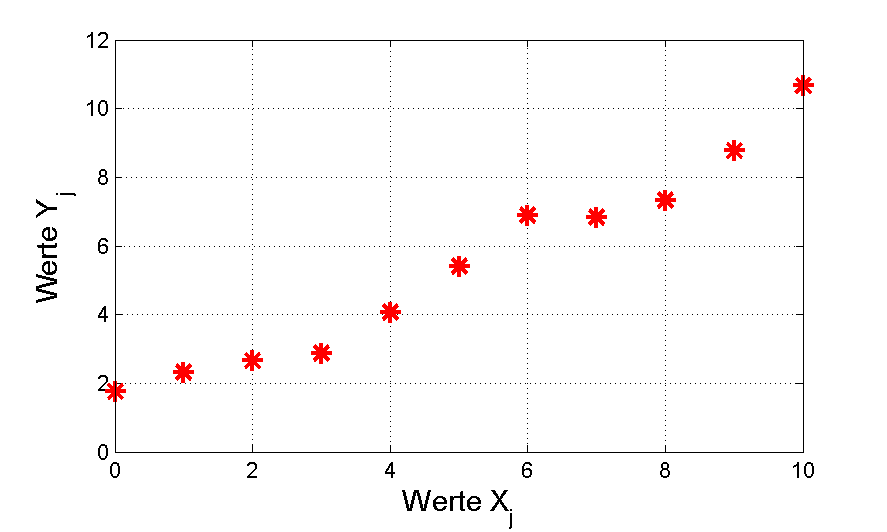
\includegraphics[width=12cm]{./Bilder/WertePaare_fuer_Regression.png}
%	\caption{Gegebene Wertepaare $X_j, Y_j$} \label{fig:Messwertpaare}
%\end{figure}

\section{Beispiele zur linearen Regression}
\label{subsection:lineare-Regression}
\textbf{Beispiel:} Vergleich der Modellierung mit Gerade und mit Polynom 6.~Grades \\
Gegeben sei ein Ensemble von Werten
$(X_j,Y_j )$, $j = 1,2,\ldots ,J$ einer Eingangsgröße (Regressor) $X$ und einer Zufallsgrößen,
der abhängigen Ausgangsgröße (Regressand) $Y$.
Beispielhaft ist in Abb.~\ref{fig:LineareRegression} eine
entsprechende Punktwolke dargestellt:
\begin{figure}[!htbp]
	\centering
	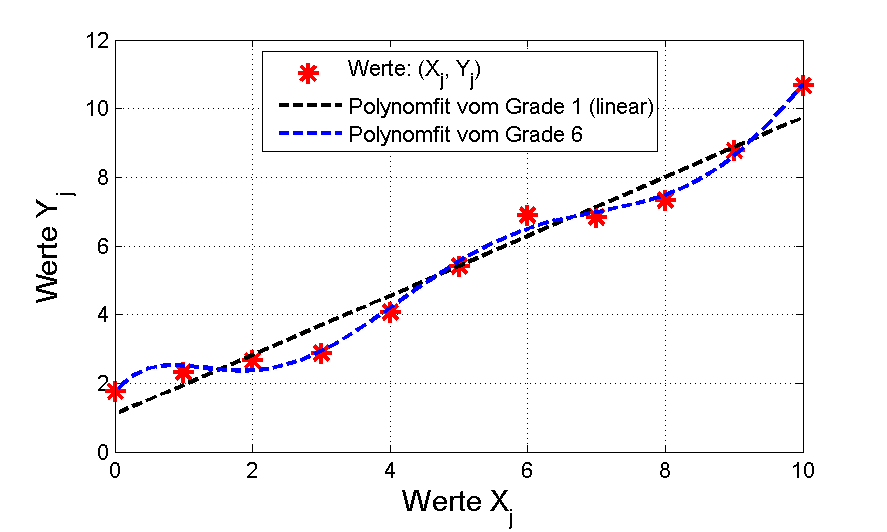
\includegraphics[width=11cm]{02_vorlesung/media/Regression_der_WertePaare.png}
    \caption{Beispiel für mögliche Fits, linearer Fit und Polynomfit vom Grade 6} \label{fig:LineareRegression}
\end{figure}
Bevor man mit der Regressionsrechnung anfängt, muss man sich im vorhinein sehr sorgfältig
überlegen, in welchem physikalischen Zusammenhang die Größen stehen, also welcher
Ansatz für das Messsystem als Modellgleichung sinnvoll ist.
In einigen Fällen ist dies auch eine Frage, welche Näherung für welchen Messbereich
ausreicht. Abb.~\ref{fig:LineareRegression} illustriert die Abweichung der Wertepaare von den unterschiedlichen Modellen und damit wie gut verschiedene Modelle die Daten approximieren.

\textbf{Beispiel:} Bestimmung des Widerstandes $R$ durch lineare Regression \\
Wir erinnern uns wieder an das Beispiel aus der 1. Vorlesung (siehe z.~B. dort Abb.~1) und bestimmen den Ohmschen Widerstand $R$ sowie eine Offsetspannung $U_0$ bei gegebenen Werten einer
Präzisions\-strom\-quelle (Regressor, genau bekannt, d.h.\ keine Zufallsgröße) und beobachteten
Werten eines Voltmeters (Regressand, Zufallsgröße). 
Der Ohmsche Widerstand $R$ und die Offsetspannung $U_0$ sind die zu bestimmenden Modellparameter (Zufallsgrößen)

\begin{center}
	\begin{tabular}{l||c|c|c|c|c|c|c|c|c}
			\hline\hline
			$I$ in mA &    4.0 &     6.0 &     8.0 &    10.0 &    12.0 &    14.0 &    16.0 &    18.0 &    20.0\\
			\hline
			$U$ in mV &    62.5 &    51.5 &    96.0 &   140.2 &   138.9 &   195.1 &   225.8 &   207.8 &   223.7 \\
			\hline\hline
	\end{tabular}
\end{center}

Die Modellgleichung lautet mit den beiden Modellparametern 
$\theta_0 :=U_0$ und $\theta_1:=R$ 
\begin{equation}
U = U_0 + R \cdot I
\end{equation}

Die beiden Modellparameter können wir mit den beiden Gleichungen (siehe Gl. (\ref{eq:Lineare_Regressionskonstanten})) bestimmt werden.
\begin{equation}
\hat{U}_0 = \bar {U} - \hat{R} \bar {I} \quad \mathrm{und} \quad
\hat{R} = \frac{s_{IU} }{s_I^2 }
\label{eq:Lineare_Regressionskonstanten_Widerstand}
\end{equation}
Zunächst bestimmen wir die beiden Mittelwerte:
\begin{equation}
\bar{I}\; := \; \frac{1}{J} \, \sum\limits_{j = 1}^J \, I_j
= 12 \, \mathrm{mA}
\qquad 
\bar{U} \; := \; \frac{1}{J} \, \sum\limits_{j = 1}^J \, U_j
= 149.0556  \, \mathrm{mV}
\end{equation}
\begin{figure}
	\centering
	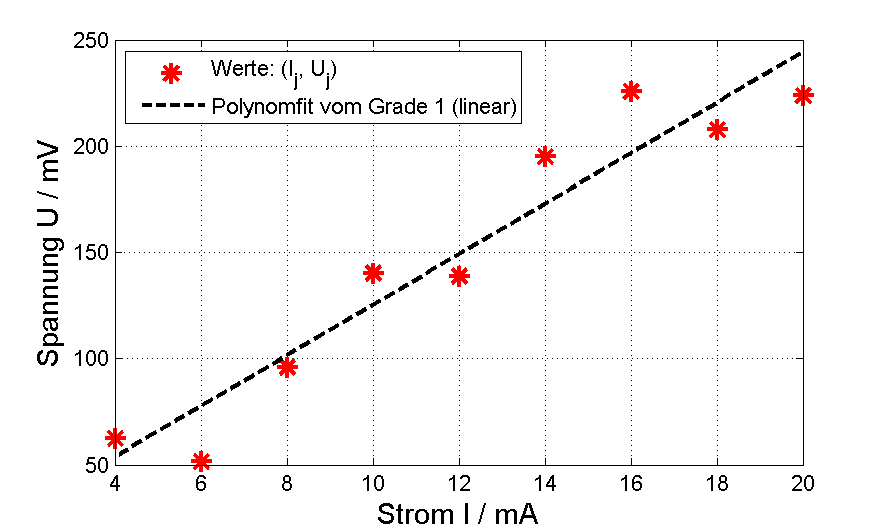
\includegraphics[width=11cm]{02_vorlesung/media/Regression_der_WertePaare_Strom_Spannung.png}
	\caption{Beispiel: Bestimmung des Ohmschen Widerstand und einer Offset-Spannung durch lineare Regression} \label{fig:LineareRegressionWiderstand}
\end{figure}
Die empirische Kovarianz mit den $J = 9$ Stichproben ergibt sich zu: 
\[
s_{IU} = \frac{1}{J - 1}\sum\limits_{j = 1}^J 
(I_j - \bar {R})(U_j - \bar {U}) = 357.0500  \, \mathrm{mA} \cdot \mathrm{mV}
\]

Die Varianz ergibt sich zu: 
\[
s_I^2 = \frac{1}{J - 1}\sum\limits_{j = 1}^J {(I_j - \bar {I})^2} = 30  \, \mathrm{mA}^2
\]

Somit erhalten wir als Schätzwert für $R$
\[
\hat{R} = \frac{s_{IU} }{s_I^2} = \frac{357.050 \, \mathrm{mA} \cdot \mathrm{mV}}{30 \, \mathrm{mA}^2} = 11.9017 
\, \frac{\mathrm{mV}}{\mathrm{mA}}
\]
mit $\frac{\mathrm{mV}}{\mathrm{mA}} = \frac{\mathrm{V}}{\mathrm{A}} = \mathrm{\Omega}$ also $\hat{R} = 11.9017 \, \mathrm{\Omega}$
und als Schätzwert für $U_0$: 
\[
\hat{U}_0 = \bar {U} - \hat{R} \bar {I} = 149.0556 \, \mathrm{mV}-  11.9017  \, \mathrm{\Omega} \cdot 12 \, \mathrm{mA} =
6.2356 \, \mathrm{mV}
\]

Das Ergebnis für die Regressionsgerade lautet somit
\begin{equation}
U = 6.2356  \, \mathrm{mV} + (11.9017 \, \mathrm{\Omega}) \cdot I 
\end{equation}
 und ist in Abb.~\ref*{fig:LineareRegressionWiderstand} dargestellt.

\section{Varianz der Regressionsparameter}
\label{subsec:vertrauensbereiche}

Es können aus den Messreihen die Varianzen der
geschätzten Regressionsparameter ermittelt werden. Das Verfahren zeigen wir
hier anhand der Regressionsgeraden mit den geschätzten Parametern
Achsenabschnitt $\hat{\theta}_0 $ und Steigung $\hat\theta_1 $.
Die Varianz der Schätzer liefert ein Ma{\ss} f\"{u}r die statistische
Sicherheit der Sch\"{a}tzung der Parameter $\theta _0 $ und
$\theta _1 $.
Für die Varianz des Regressionsparameters Steigung $\hat{\theta}_1 $
gilt:
\begin{equation}
\sigma^2_{\hat{\theta}_1} = \frac{ \hat \sigma^2_{\varepsilon}}{s^2_X \cdot (J- 1) }
\end{equation}

Für die Varianz des Regressionsparameters Achsenabschnitt $\hat{\theta}_0 $
gilt:
\begin{equation}
\sigma^2_{\hat{\theta}_0} = \hat \sigma^2_{\varepsilon} \cdot \left(\frac{1}{J}
	+ \frac{\bar {X}^2}{(J - 1) s_X^2 }\right)^2
\end{equation}
\begin{center}
\end{center}

Die Varianz des Achsenabschnittes wird weiter unten in der Gl.(\ref{eq:Varianz des Achsenabschnitts}) hergeleitet. Dort ergibt sich \begin{equation}
\hat \sigma^2_{\theta_0}  = \hat \sigma^2_{\varepsilon}  \sum(X_j^2)  / (J \sum(X_j^2) - (\sum(X_j))^2) 
\end{equation}
Wir bezeichnen nun das $\hat \sigma^2_{\varepsilon}$ hier mit $s^2_{\varepsilon}$ und erhalten:
\begin{equation}
\hat \sigma^2_{\theta_0}  = s^2_{\varepsilon} \sum(X_j^2)  / (J \sum(X_j^2) - (\sum(X_j))^2) 
\end{equation}
\begin{equation}
\hat \sigma^2_{\theta_0} = s^2_{\varepsilon} \frac{1}{J} \sum(X_j^2)  / (\sum(X_j^2) - \frac{1}{J}(\sum(X_j))^2)
\end{equation}
Mit der folgenden Null-Identität
\begin{equation}
0 =  - \frac{1}{J}(\sum(X_j))^2 + \frac{1}{J}(\sum(X_j))^2
\end{equation}
gilt
\[
(1/J) \sum(X_j^2)  / (\sum(X_j^2) - \frac{1}{J}(\sum(X_j))^2) = 
\]
\[
(1/J) [\sum(X_j^2) - (1/J)(\sum(X_j))^2 + \frac{1}{J}(\sum(X_j))^2] / (\sum(X_j^2) - (1/J)(\sum(X_j))^2)
\]
das heisst
\[
\frac{1}{J} \sum(X_j^2)  / (\sum(X_j^2) - \frac{1}{J}(\sum(X_j))^2) =
\]
\[
(1/J) [ 1 + \frac{1}{J}(\sum(X_j))^2 / (\sum(X_j^2) - \frac{1}{J}(\sum(X_j))^2) ]
\]

und mit $(\sum(X_j^2) - \frac{1}{J}(\sum(X_j))^2) = (J-1) s_X^2$ gilt dann
\begin{align}
\hat \sigma^2_{\theta_0} =& 
s^2_{\varepsilon} \frac{1}{J} \sum(X_j^2)  / (\sum(X_j^2) - \frac{1}{J}(\sum(X_j))^2) \\
=& s^2_{\varepsilon} \frac{1}{J} \sum(X_j^2)  / (J-1) s_X^2
\end{align}
und mit der Umformung der Null-Identität gilt dann
\begin{align}
\hat \sigma^2_{\theta_0} 
=& s^2_{\varepsilon} \frac{1}{J} \sum(X_j^2)  / (\sum(X_j^2) - \frac{1}{J}(\sum(X_j))^2) \\
=& s^2_{\varepsilon} \frac{1}{J} \left[ 1 + \frac{1}{J}(\sum(X_j))^2 / (\sum(X_j^2) - \frac{1}{J}(\sum(X_j))^2) \right] \\
=& s^2_{\varepsilon} \frac{1}{J} \left[ 1 + \frac{1}{J(J-1) s_X^2} \left(\sum(X_j)\right)^2 \right]  
\end{align}
mit $\frac{1}{J}(\sum(X_j)) = \bar X$ gilt $\frac{1}{J}(\sum(X_j))^2 = J \bar X^2$
so dass
\begin{align}
\hat \sigma^2_{\theta_0} =& s_{\varepsilon} \frac{1}{J} \left[ 1 + 
\frac{1}{J (J-1) s_X^2} \left(\sum(X_j) \right)^2 \right] \\
=& s^2_{\varepsilon} \frac{1}{J(J-1) s_X^2} \left[ 1 + (J \bar X^2) \right] \\
=&
s^2_{\varepsilon}  \left[\frac{1}{J} + \frac{\bar X^2}{(J-1) s_X^2} \right]
\end{align}

Damit erhalten wir für die \textbf{Varianz bzw. die Unsicherheit des Achsenabschnittes}: 
\begin{equation}
\hat \sigma^2_{\theta_0} =
s^2_{\varepsilon}  \left[ \frac{1}{J} +\frac{\bar {X}^2}{(J - 1) s_X^2 } \right]
\end{equation}

\section{Matrixformalismus zur allgemeinen Lösung der linearen Regression}

\subsection{Matrixformalismus anhand der Regressionsgeraden}

Als Regressormatrix verwenden wir jetzt
\begin{equation}
\mathbf{X} \; = \;
\left(
\begin{array}{cc}
1 &  X_{1,1} \\
\vdots & \vdots\\
1 & X_{1,J} 
\end{array}
\right)
\end{equation}
Die Residuen berechnen sich wie folgt: 
\begin{equation}
\left(
\begin{array}{c}
\varepsilon_1\\
\vdots \\
\varepsilon_J
\end{array}
\right)  \; = \;
\left(
\begin{array}{c}
Y_{1} \; - \; (1 \, \theta_0 \; + \;  X_{1,1} \, \theta_1)\\
\vdots \\
Y_{J} \; - \; (1 \, \theta_0 \; + \;  X_{1,J} \, \theta_1)
\end{array}
\right) \; = \;
\left(
\begin{array}{c}
Y_{1}\\
\vdots \\
Y_{J}
\end{array}
\right) 
\; - \; 
\left(
\begin{array}{cc}
1 &  X_{1,1} \\
\vdots & \vdots\\
1 & X_{1,J} 
\end{array}
\right) 
\left(
\begin{array}{c}
\theta_0\\
\theta_1
\end{array}
\right)
\label{linearRegressionGeradeTheta}
\end{equation}
Die Summe der Quadrate der Residuen $\sum_{j=1}^J \varepsilon_j^2$ lässt sich ebenso
mit der Rechenregel Zeile mal Spalte schreiben, als Zeilenvektor mal Spaltenvektor
\begin{equation}
\sum_{j=1}^J \varepsilon_j^2 \; = \; 
\left(\begin{array}{ccc}
\varepsilon_1 & \dots & \varepsilon_J
\end{array}
\right)
\left(
\begin{array}{c}
\varepsilon_1\\
\vdots \\
\varepsilon_J
\end{array}
\right)
\end{equation}
Dabei heißt der Zeilenvektor der transponierte Vektor, also
\begin{equation}
\boldsymbol{\varepsilon}^\mathsf{T} \; = \; \left(\begin{array}{ccc}
\varepsilon_1 & \dots & \varepsilon_J
\end{array}
\right) \qquad \mathrm{und}  \qquad 
\boldsymbol{\varepsilon} \; = \; \left(
\begin{array}{c}
\varepsilon_1\\
\vdots \\
\varepsilon_J
\end{array}
\right)
\end{equation}
und ferner führen wir ein
\begin{equation}
\boldsymbol{\theta} \; = \;
\left(
\begin{array}{c}
\theta_0\\
\theta_1
\end{array}
\right) \qquad \mathrm{und}  \qquad 
\mathbf{Y}  \; = \;\left(
\begin{array}{c}
Y_{1}\\
\vdots \\
Y_{J}
\end{array}
\right) 
\end{equation}
und Gl.~(\ref{linearRegressionGeradeTheta}) sieht in transponierter Schreibweise
wie folgt aus
\begin{equation}
\boldsymbol{\varepsilon}^\mathsf{T} \; = \;
\mathbf{Y}^\mathsf{T}
\; - \; 
\boldsymbol{\theta}^\mathsf{T} \left(
\begin{array}{cc}
1 &  X_{1,1} \\
\vdots & \vdots\\
1 & X_{1,J} 
\end{array}
\right)^\mathsf{T} 
\label{linearRegressionGeradeTransponiert}
\end{equation}
d.h.
\begin{equation}
\boldsymbol{\varepsilon}^\mathsf{T} \; = \;
\mathbf{Y}^\mathsf{T}
\; - \; 
\left(
\begin{array}{cc}
\theta_0 &
\theta_1
\end{array}
\right) \left(
\begin{array}{ccc}
1 &  \dots & 1 \\
X_{1,1} & \dots & X_{1,J} 
\end{array}
\right).
\label{linearRegressionGeradeUmform}
\end{equation}
Die Summe der Quadrate der Residuen $\sum_{j=1}^J \varepsilon_j^2$  sieht damit wie
folgt aus
\begin{equation}
\boldsymbol{\varepsilon}^\mathsf{T}  \boldsymbol{\varepsilon} \; = \;
\left(
\mathbf{Y}^\mathsf{T}
\; - \; 
\boldsymbol{\theta}^\mathsf{T} \mathbf{X}^\mathsf{T} \right)
\left(
\mathbf{Y}
\; - \; 
\mathbf{X} \boldsymbol{\theta} \right)
\end{equation}
d.h.
\begin{equation}
\boldsymbol{\varepsilon}^\mathsf{T}  \boldsymbol{\varepsilon} \; = \;
\mathbf{Y}^\mathsf{T} \mathbf{Y}
\; - \; 
\boldsymbol{\theta}^\mathsf{T} \mathbf{X}^\mathsf{T}  \mathbf{Y} 
\; - \; 
\mathbf{Y}^\mathsf{T}  \mathbf{X} \boldsymbol{\theta}
\; + \; 
\boldsymbol{\theta}^\mathsf{T} \mathbf{X}^\mathsf{T} \mathbf{X} \boldsymbol{\theta}
\end{equation}
Für die Ableitungen nach den $\theta_0, \theta_1$ gilt
\begin{equation}
\frac{\partial}{\partial \theta_l} \sum_{j=1}^J \varepsilon_j^2 \; = \; 
2 \sum_{j=1}^J \varepsilon_j \frac{\partial}{\partial \theta_l} \varepsilon_j \; = \; 
2 \sum_{j=1}^J \varepsilon_j (-1) \frac{\partial}{\partial \theta_l}(1 \, \theta_1 \; + \;  X_{1,j} \, \theta_2) \; = \; 0
\end{equation}
wobei $l = 0,1$ ist also
\begin{equation}
\sum_{j=1}^J \varepsilon_j  \frac{\partial}{\partial \theta_0}(1 \, \theta_0 \; + \;  X_{1,j} \, \theta_1)  \; = \; 0 \qquad \mathrm{und} \qquad 
\sum_{j=1}^J \varepsilon_j  \frac{\partial}{\partial \theta_1}(1 \, \theta_0 \; + \;  X_{1,j} \, \theta_1)  \; = \; 0
\end{equation}
also
\begin{equation}
\sum_{j=1}^J \varepsilon_j (1) \; = \; 0 \qquad \mathrm{und}  \qquad 
\sum_{j=1}^J \varepsilon_j ( X_{1,j})  \; = \; 0
\end{equation}
Dies sieht in Matrixschreibweise als $2 \times 2$-Gleichungssystem wie folgt aus
\begin{equation}
\boldsymbol{\varepsilon}^\mathsf{T} \, \mathbf{X} \; = \;
\left(
\begin{array}{c}
0\\
0
\end{array}
\right)
\end{equation}
d.h.
\begin{equation}
\left(\mathbf{Y}^\mathsf{T}
\; - \; 
\boldsymbol{\theta}^\mathsf{T} \mathbf{X}^\mathsf{T} \right) \, \mathbf{X} \; = \;
\left(
\begin{array}{c}
0\\
0
\end{array}
\right)
\end{equation}
d.h.
\begin{equation}
\boldsymbol{\theta}^\mathsf{T} \, \mathbf{X}^\mathsf{T}  \, \mathbf{X} \; = \;
\mathbf{Y}^\mathsf{T} \, \mathbf{X}
\end{equation}
%$\frac{\partial}{\partial \beta_l} \varepsilon_j$ auf.
%Der Vektor mit für die partielle Differentiation heißt Nablaoperator
%\begin{equation}
%\nabla_\beta \; = \;
%\left(
%\begin{array}{cc}
%\frac{\partial}{\partial \beta_0} &
%\frac{\partial}{\partial \beta_1}
%\end{array}
%\right)
%\end{equation}
das ist äquivalent zu
\begin{equation}
\mathbf{X}^\mathsf{T} \, \mathbf{X} \, \boldsymbol{\theta} \; = \;
\mathbf{X}^\mathsf{T} \, \mathbf{Y} .
\end{equation}
Die numerische Lösung des Gleichungssystems liefert dann die Schätzwerte zu
den Regressionparametern $\boldsymbol{\theta}$. Ein mögliches Verfahren zum
Lösen des linearen Gleichungssystems ist das Gauß-Jordan-Eliminationsverfahren, zu
dem im Anhang dieses Skripts der Quellcode gemäß den \textsl{Numerical Recipes}
\cite{Fla02} abgedruckt ist.
Formal notieren wir 
die Schätzer (als solche kenntlich durch das Dach) wie folgt
\begin{equation}
\boldsymbol{\hat \theta} \; = \;
\left( \mathbf{X}^\mathsf{T}  \, \mathbf{X} \right)^{-1} \mathbf{X}^\mathsf{T} \, \mathbf{Y}
\end{equation}
wobei hoch minus Eins soviel bedeutet wie die Inverse der Matrix.

Als nächstes ermitteln wir, um das \textbf{vollständige
	Messergebnis} zu erhalten, auch die Schätz\-werte der Kovarianzen. Die
Hauptdiagonale der Kovarianzmatrix sind die Varianzen.
\begin{equation}
\operatorname {Cov}( \boldsymbol{\theta},\boldsymbol{\theta} ) \; = \;
\operatorname {Cov} 
\left(\left( \mathbf{X}^\mathsf{T}  \, \mathbf{X} \right)^{-1} \mathbf{X}^\mathsf{T} \, \mathbf{Y}, \left( \mathbf{X}^\mathsf{T}  \, \mathbf{X} \right)^{-1} \mathbf{X}^\mathsf{T} \, \mathbf{Y}\right)
\end{equation}
%mit Gl.~(\ref{CovarianzKonstMatrix}) ist dies
das ist
\begin{equation}
\operatorname {Cov}( \boldsymbol{\theta}, \boldsymbol{\theta} ) \; = \;
\left( \mathbf{X}^\mathsf{T}  \, \mathbf{X} \right)^{-1} \mathbf{X}^\mathsf{T} \operatorname {Cov} (\mathbf{Y}, \mathbf{Y}) \, \left( \left( \mathbf{X}^\mathsf{T}  \, \mathbf{X} \right)^{-1} \mathbf{X}^\mathsf{T} \right)^\mathsf{T}
\end{equation}
und mit Einsetzen der aus den Schätzern $\boldsymbol{\hat \theta}$ erhaltenen
empirischen Varianz der Residuen 
$\operatorname {Cov} (\mathbf{Y}, \mathbf{Y}) = \operatorname {Var} (\mathbf{\varepsilon}) = \hat \sigma_{\varepsilon}^2$
bekommen wir die empirische Kovarianzmatrix
\begin{equation}
\boldsymbol{\hat \Sigma}_{\boldsymbol{\theta}} \; = \;
\hat \sigma_{\varepsilon}^2
\left( \mathbf{X}^\mathsf{T}  \, \mathbf{X} \right)^{-1} \mathbf{X}^\mathsf{T} \, \left( \left( \mathbf{X}^\mathsf{T}  \, \mathbf{X} \right)^{-1} \mathbf{X}^\mathsf{T} \right)^\mathsf{T}
\end{equation}
mit
$$
\operatorname {Var} (\mathbf{\varepsilon}) = \hat \sigma_{\varepsilon}^2 \; = \;
\frac{1}{J-M} \, \boldsymbol{\hat \varepsilon}^\mathsf{T} \boldsymbol{\hat \varepsilon}
$$
wobei $M$ die Anzahl der Regressionsparameter ist, also $M = 2$ im Fall der Geraden, für die beiden Parameter Achsenabschnitt und Steigung und
$$
\boldsymbol{\hat \varepsilon} \; = \; \mathbf{Y} \, - \, \mathbf{X} \boldsymbol{\hat \theta} .
$$

Ferner gilt mit $\left( \left( \mathbf{X}^\mathsf{T}  \, \mathbf{X} \right)^{-1} \mathbf{X}^\mathsf{T} \right)^\mathsf{T} = \mathbf{X} \left( \mathbf{X}^\mathsf{T}  \, \mathbf{X} \right)^{-1}$
\begin{equation}
\boldsymbol{\hat \Sigma}_{\boldsymbol{\theta}} \; = \; \hat \sigma_{\varepsilon}^2
\left( \mathbf{X}^\mathsf{T}  \, \mathbf{X} \right)^{-1} \mathbf{X}^\mathsf{T}  \,  \mathbf{X} \, \left( \mathbf{X}^\mathsf{T}  \, \mathbf{X} \right)^{-1} 
\end{equation}
und mit $\left( \mathbf{X}^\mathsf{T}  \, \mathbf{X} \right)^{-1} \mathbf{X}^\mathsf{T}  \, \mathbf{X}  \; = \; 1 \! \mathrm{I}$ Einheitsmatrix
\begin{equation}
\boldsymbol{\hat \Sigma}_{\boldsymbol{\theta}} \; = \; \hat \sigma_{\varepsilon}^2
\left( \mathbf{X}^\mathsf{T}  \, \mathbf{X} \right)^{-1}
\label{UnsicherheitRegressparams}
\end{equation}
Gleichung (\ref{UnsicherheitRegressparams}) liefert die Unsicherheit für die Regressionsparameter
$\boldsymbol{\theta}$. 
%Sie unterscheidet sich
%Gleichung (\ref{KovarianzSumme})
Setzen wir dies nun für die Regressionsgerade ein, also setzen wir
$$
\mathbf{X} \; = \;
\left(
\begin{array}{cc}
1 &  X_{1,1} \\
\vdots & \vdots\\
1 & X_{1,J} 
\end{array}
\right)
$$
ein, so erhalten wir für
\begin{equation}
\left( \mathbf{X}^\mathsf{T}  \, \mathbf{X} \right)^{-1} \; = \;
\left( \left(
\begin{array}{ccc}
1 & \cdots & 1 \\
X_{1,1} & \cdots & X_{1,J} 
\end{array}
\right)
\, 
\left(
\begin{array}{cc}
1 &  X_{1,1} \\
\vdots & \vdots\\
1 & X_{1,J} 
\end{array}
\right) \right)^{-1}
\end{equation}
d.h.
\begin{equation}
\left( \mathbf{X}^\mathsf{T}  \, \mathbf{X} \right)^{-1} \; = \;
\left(
\begin{array}{ccc}
J & \sum\limits_{j=1}^J X_{1,j} \\
\sum\limits_{j=1}^J X_{1,j} & \sum\limits_{j=1}^J X_{1,j}^2
\end{array}
\right)^{-1}
\end{equation}
d.h.
\begin{equation}
\left( \mathbf{X}^\mathsf{T}  \, \mathbf{X} \right)^{-1} \; = \;
\frac{1}{J \, \sum\limits_{j=1}^J X_{1,j}^2 \; - \;
	\left(\sum\limits_{j=1}^J X_{1,j}\right)^2}
\left(
\begin{array}{ccc}
\sum\limits_{j=1}^J X_{1,j}^2 & -\sum\limits_{j=1}^J X_{1,j} \\
-\sum\limits_{j=1}^J X_{1,j} & J
\end{array}
\right)
\end{equation}
so dass wir für den Achsenabschnitt $\theta_0$ und die Steigung $\theta_1$ folgende
empirische Varianzen und Kovarianzen erhalten
\begin{equation}
\left(\begin{array}{cc}
\hat \sigma^2_{\theta_0} &\hat \sigma_{\theta_0, \theta_1}\\
\hat \sigma_{\theta_0, \theta_1} & \hat \sigma^2_{\theta_1} 
\end{array}\right)
\; = \;
\frac{\hat \sigma^2_\varepsilon}{J \, \sum\limits_{j=1}^J X_{1,j}^2 \; - \; 
	\left(\sum\limits_{j=1}^J X_{1,j}\right)^2}
\left(
\begin{array}{ccc}
\sum\limits_{j=1}^J X_{1,j}^2 & -\sum\limits_{j=1}^J X_{1,j} \\
-\sum\limits_{j=1}^J X_{1,j} & J
\end{array}
\right)
\end{equation}
oder einzeln aufgeschrieben, die Varianz des Achsenabschnitts
%\begin{figure}
%	\begin{center}
%		\includegraphics[width=100mm]{Bilder/regressionNormalResi_Perr_1a.eps}
%		\caption{\label{regressionParamErr} Unsicherheit der Schätzer
%			der linearen Regression einer Geradengleichung für ein
%			Vertrauensniveau von $98 \%$. Mit $\nu = J-2 = 26-2 = 24$ Freiheitsgraden
%			ist das Quantil der Student-t-Verteilung $t_{1-\alpha/2,\nu} = 2.492$.}
%	\end{center}
%\end{figure}
\begin{equation}
\hat \sigma^2_{\theta_0} \; = \; 
\frac{\hat \sigma^2_\varepsilon \, \sum\limits_{j=1}^J X_{1,j}^2}{J \, 
	\sum\limits_{j=1}^J X_{1,j}^2 \; - \; \left(\sum\limits_{j=1}^J X_{1,j}\right)^2}
\label{eq:Varianz des Achsenabschnitts}
\end{equation}
die Kovarianz für Achsenabschnitt und Steigung
\begin{equation}
\hat \sigma_{\theta_0, \theta_1} \; = \; 
\frac{- \hat \sigma^2_\varepsilon \, \sum\limits_{j=1}^J X_{1,j}}{J \, \sum_{j=1}^J X_{1,j}^2 \;
	- \; \left(\sum\limits_{j=1}^J X_{1,j}\right)^2}
\end{equation}
und die Varianz der Steigung
\begin{equation}
\hat \sigma^2_{\theta_1} \; = \; 
\frac{\hat \sigma^2_\varepsilon}{\sum\limits_{j=1}^J X_{1,j}^2 \; - \; 
	\frac{1}{J}\left(\sum\limits_{j=1}^J X_{1,j}\right)^2} .
\end{equation}
Die Standardabweichungen zu jedem Regressionsparameter $\theta_l$ mit $l = 0,\dots,M-1$ sind
die Wurzel aus den Varianzen, die auf der Hauptdiagonalen der Kovarianzmatrix 
$\left( \mathbf{X}^\mathsf{T}  \, \mathbf{X} \right)^{-1} \, \hat \sigma_{\varepsilon}^2$
stehen. In der üblichen englischsprachigen Literatur zur Regressionrechnung wird
die Standardabweichung der Regressionsparameter \textsl{Standard Error} genannt.

\subsection{Matrixansatz als allgemeiner Ansatz für linearen Regression}

Die behandelten allgemeinen Formen von Problemstellungen zur Schätzung von Modellparametern
werden wir in dieser Vorlesungsreihe nicht weiter vertiefen. Sie sollen lediglich einen Einblick
und Überblick über die vielfältigen Möglichkeiten in diesem Bereich liefern.
In den Übungen und der Klausur werden
wir uns auf das Schätzverfahren mittels linearer Regression fokussieren.


Um die lineare Regression universeller einsetzen zu können, ob nun Polynome oder
Ebenen oder Paraboloide zu fitten sind, ist es erforderlich den allgemeinen Ansatz zu verstehen
und die unterschiedlichen Anwendungen so formulieren zu können, dass sie darüber lösbar werden.

Wir wollen also den Übergang von Gl.~(\ref{linearRegressionGeradeTheta}) mit
\begin{equation*}
\left(
\begin{array}{c}
\varepsilon_1\\
\vdots \\
\varepsilon_J
\end{array}
\right)  \; = \;
\left(
\begin{array}{c}
 Y_{1} \; - \; (1 \, \theta_0 \; + \;  X_{1,1} \, \theta_1)\\
\vdots \\
 Y_{J} \; - \; (1 \, \theta_0 \; + \;  X_{1,J} \, \theta_1)
\end{array}
\right) \; = \;
\left(
\begin{array}{c}
 Y_{1}\\
\vdots \\
 Y_{J}
\end{array}
\right) 
\; - \; 
\left(
\begin{array}{cc}
 1 &  X_{1,1} \\
\vdots & \vdots\\
 1 & X_{1,J} 
\end{array}
\right) 
\left(
\begin{array}{c}
\theta_0\\
\theta_1
\end{array}
\right)
\end{equation*}
mit
\begin{equation*}
\mathbf{X} \; = \;
\left(
\begin{array}{cc}
 1 &  X_{1,1} \\
\vdots & \vdots\\
 1 & X_{1,J} 
\end{array}
\right)
\end{equation*}
zu einer allgemeinen Formulierung finden.

Für $M$ Regressoren wird die Regressormatrix zu einer $J \times M$-Matrix, also einer Matrix
aus $M$ Spalten und $J$ Zeilen aufgestellt:
\begin{equation}
\mathbf{X} \; = \;
\left(
\begin{array}{ccc}
 X_{1,1} & \dots &  X_{M,1} \\
\vdots & & \vdots \\
 X_{1,J}  & \dots &  X_{M,J}
\end{array}
\right)
\end{equation}
Die Indexschreibweise ist hier relativ zur Schreibweise der Matrizenrechnung vertauscht, weil wir den Index für die
Messgrößen vorne haben gefolgt von dem Index für die Beobachtungen, wir aber die Messgrößen als
Spaltenvektoren verwenden und somit den Index für die Beobachtungen als Zeilenindex haben.

\begin{equation}
\boldsymbol{\varepsilon} \, =  \, \left(
\begin{array}{c}
\varepsilon_1\\
\vdots \\
\varepsilon_J
\end{array}
\right)  \; = \;
\left(
\begin{array}{c}
 Y_{1} \; - \; (X_{1,1} \, \theta_1  \; + \; \dots  \; + \;  X_{M,1} \, \theta_{M})\\
\vdots \\
 Y_{J} \; - \; (X_{1,J} \, \theta_1 \; + \; \dots  \; + \;  X_{M,J} \, \theta_{M})
\end{array}\right)  \, = \, 
\mathbf{Y} \, -  \, \mathbf{X} \, \boldsymbol{\theta}
\end{equation}
Im Fall eines Polynoms kann jeder der Regressoren Funktion derselben Messgröße sein.
Dies kann beispielsweise einfach
durch folgenden Potenzansatz $X_{m,j} = X_{1,j}^{m-1}$ mit $m = 1,\dots,M$ als
Polynom vom Grad $M-1$ dargestellt werden
\begin{equation}
\left(
\begin{array}{c}
\varepsilon_1\\
\vdots \\
\varepsilon_J
\end{array}
\right)  \; = \;
\left(
\begin{array}{c}
 Y_{1} \; - \; (X_{1,1}^0 \, \theta_1  \; + \; \dots  \; + \;  X_{1,1}^{M-1} \, \theta_{M})\\
\vdots \\
 Y_{J} \; - \; (X_{1,J}^0 \, \theta_1 \; + \; \dots  \; + \;  X_{1,J}^{M-1} \, \theta_{M})
\end{array}\right)
\end{equation}
wobei $X_{1,j}^0 = 1$ ist.

Wird die Regressormatrix zu Beginn korrekt aufgestellt, so lassen sich die 
$M$ Regressionsparameter $\boldsymbol{\theta}$
schätzen durch numerische Lösung des folgenden Gleichungssystems:
\begin{equation}
\mathbf{X}^\mathsf{T} \, \mathbf{X} \, \boldsymbol{\theta} \; = \;
\mathbf{X}^\mathsf{T} \, \mathbf{Y} .
\label{LsgRegressionGlSys}
\end{equation}
Dass nach Lösen des Gleichungssystems Schätzwerte für
die Parameter gewonnen wurden, wird durch das Dach auf dem Symbol $\boldsymbol{\theta}$ gekennzeichnet.
\begin{equation}
 \boldsymbol{\hat \theta} \; = \;
\left( \mathbf{X}^\mathsf{T}  \, \mathbf{X} \right)^{-1} \mathbf{X}^\mathsf{T} \, \mathbf{Y}
\end{equation}
wobei hoch minus Eins soviel bedeutet wie die Inverse der Matrix.
Für Varianzen und Kovarianzen der $M$ Regressionsparameter $\theta_1, \dots, \theta_M$
werden die Residuen gebraucht
\begin{equation}
\boldsymbol{\hat \varepsilon} \, =  \, \left(
\begin{array}{c}
\hat \varepsilon_1\\
\vdots \\
\hat \varepsilon_J
\end{array}
\right)  \; = \;
\left(
\begin{array}{c}
 Y_{1} \; - \; (X_{1,1} \, \hat \theta_1  \; + \; \dots  \; + \;  X_{M,1} \, \hat \theta_{M})\\
\vdots \\
 Y_{J} \; - \; (X_{1,J} \, \hat \theta_1 \; + \; \dots  \; + \;  X_{M,J} \, \hat \theta_{M})
\end{array}
\right) \, = \, 
\mathbf{Y} \, -  \, \mathbf{X} \, \boldsymbol{\hat \theta}
\end{equation}
um deren empirische Varianz zu berechnen
\begin{equation}
\hat \sigma_{\varepsilon}^2 \; = \;
\frac{1}{J-M} \, \boldsymbol{\hat \varepsilon}^\mathsf{T} \boldsymbol{\hat \varepsilon}
\end{equation}
so dass wir die empirische Kovarianzmatrix der Parameter gmäß Gl.~(\ref{UnsicherheitRegressparams}) erhalten:
\begin{equation*}
\boldsymbol{\hat \Sigma}_{\boldsymbol{\theta}} \; = \; 
\left( \mathbf{X}^\mathsf{T}  \, \mathbf{X} \right)^{-1} \;
\hat \sigma_{\varepsilon}^2
\end{equation*}
Um die Unsicherheit der einzelnen Regressionsparameter zu erhalten, führen wir Einheitsvektoren ein, die $M$-dimensional sind.
Bei dem $l$-ten Einheitsvektor sind die ersten $l-1$ Vektorkomponenten Nullen, an der $l$-ten Stelle steht eine Eins
und die $l+1$-te Komponente bis zur $M$-ten sind wieder Nullen.
\begin{equation}
\boldsymbol{e}_l \; = \;
\left(\begin{array}{c}
0\\
\vdots\\
0\\
1\\
0\\
\vdots\\
0
\end{array}\right)
\end{equation}
Dann lässt sich durch folgende Multiplikation die $l$-te Varianz, d.h. das $l$-te Element
der Hautpdiagonalen aus der Kovarianzmatrix herausholen
\begin{equation}
\hat \sigma_l^2 \; = \; \boldsymbol{e}_l^\mathsf{T} \, \left( \mathbf{X}^\mathsf{T}  \, \mathbf{X} \right)^{-1} \, \boldsymbol{e}_l  \; \hat \sigma_{\varepsilon}^2 .
\end{equation}
Die Standardabweichung (\textsl{Standard Error}) wird daraus durch Ziehen der Wurzel
gewonnen
\begin{equation}
\hat \sigma_l \; = \; \sqrt{\hat \sigma_l^2} .
\end{equation}
Im fünften Kapitel werden wir dann sehen, wie man mit Hilfe der Varianzen bzw. Standardabweichungen Vertrauensintervalle für die geschätzten Modellparameter bestimmt.

\section{Das Bestimmtheitsmaß, empirischer Korrelationskoeffizient}
Die G\"{u}te des gew\"{a}hlten linearen Ansatzes kann mit dem
\textbf{Bestimmtheitsmaß} $\rho_{XY}^2 $ bzw. dem \textbf{empirischen
Korrelationskoeffizienten} $\rho_{XY}$ beurteilt werden, aber nur dann
wenn ein solcher Zusammenhang auch existiert. Der empirische
Korrelationskoeffizienten gibt den Grad der linearen
Abh\"{a}ngigkeit zwischen den Messwerten $(X_1 ,\ldots ,X_J )$ und
$(Y_1 ,\ldots ,Y_J)$ an. 

Für den empirischen Korrelationskoeffizienten $\rho_{XY}$ gilt folgendes:

\begin{center}
	\begin{tabular}
		{|p{100pt}|p{209pt}|} \hline 
		$\rho_{XY} = \pm 1$&
		100{\%} lineare Abh\"{a}ngigkeit  \\
		\hline $\rho_{XY} = 0$&
		keine lineare Abh\"{a}ngigkeit \\
		\hline $\rho_{XY} > \mbox{bzw.} < 0$&
		gleich-/gegenl\"{a}ufige lineare Abh\"{a}ngigkeit \\
		\hline
	\end{tabular}
\end{center}

F\"{u}r die Bestimmung des Bestimmtheitsma{\ss}es oder des
empirischen Korrelationskoeffizient f\"{u}hrt man eine Streuungs-
bzw. Varianzanalyse durch. Man kann bei der linearen Regression 3
Arten von Streuungen unterscheiden:
\begin{itemize}
	\item[] $s_{\mathrm{T}}^2:$~die \textbf{totale empirische Varianz}
    \item[] $s_{\mathrm{M}}^2:$~die \textbf{empirische Varianz auf Grund des Modells}
	\item[] $s_{\mathrm{R}}^2:$~die \textbf{restliche empirische Varianz}
\end{itemize}
Die totale Streuung ist bei unabhängigen direkten Messgrößen $X_j$ gegeben
durch:
\begin{equation}
s_{\mathrm{T}}^2 = \frac{1}{J - 1}\sum\limits_{j = 1}^J {(Y_j - \bar {Y})^2}
\quad \mathrm{mit~} Y_j : \mathrm{Messwert ~zu~}  X_j 
\end{equation}
Die empirische Varianz auf Grund des Modells beschreibt die
Streuung der Y-Werte auf der Regressionsgeraden in Bezug zum
Mittelwert $\bar{Y}$, d.~h.
\begin{equation}
s_{\mathrm{M}}^2 = \frac{1}{J - 1}\sum\limits_{j = 1}^n {(\hat{\theta}_0 + \hat{\theta}_1 X_j - \bar
	{Y})^2}
\end{equation}
Die Differenz zwischen $Y_j$ und $\hat{\theta}_0 + \hat{\theta}_1 X_j $ bleiben im
Modell unerkl\"{a}rt, sie wird als restliche Streuung bezeichnet:
\begin{equation}
s_{\mathrm{R}}^2 = \frac{1}{J - 1}\sum\limits_{j = 1}^J {(Y_j - (\hat{\theta}_0 
	+ \hat{\theta}_1 X_j))^2}
\end{equation}
Man kann nun folgendes Bemerkenswerte zeigen:
\begin{equation}
s_{\mathrm{T}}^2 = s_{\mathrm{M}}^2 + s_{\mathrm{R}}^2
\end{equation}
Das Bestimmtheitsma{\ss} ist definiert als das Verh\"{a}ltnis von
empirischer Varianz des Modells zu der totalen Varianz:
\[
\rho_{XY}^2 = \frac{s_{\mathrm{M}}^2}{s_{\mathrm{T}}^2} = \frac{\sum\limits_{j = 1}^J {(\hat{\theta}_0 + \hat{\theta}_1 X_j - \bar {Y})^2} }{\sum\limits_{j = 1}^J {(Y_j - \bar{Y})^2} }
\]
Mit dem Schwerpunkt $\bar {Y} = \hat{\theta}_0 + \hat{\theta}_1 \bar {X}$ ergibt sich:
\[
\rho_{XY}^2 = \frac{\hat{\theta}_1^2 \cdot \sum\limits_{j = 1}^J 
	{(X_j - \bar X)^2} }{\sum\limits_{j = 1}^J {(Y_j - \bar {Y})^2} }
\]
Mit den Regressionsparametern $\hat{\theta}_1 = \frac{\sum\limits_{j =
		1}^J {(X_j - \bar {X})(Y_j - \bar {Y})} }{\sum\limits_{j = 1}^J {(X_j
		- \bar {X})^2} }$ (siehe Gl.(\ref{eq:Lineare_Regressionskonstanten})) erhält man für das 
	    Bestimmtheitsmaß:
\begin{align}
\rho_{XY}^2 &= \frac{\left[ {\sum\limits_{j = 1}^J {(X_j - \bar {X})(Y_j - \bar{Y})} } \right]^2}{\sum\limits_{j = 1}^J {(X_j - \bar {X})^2}
	\cdot
	\sum\limits_{j = 1}^J {(Y_j - \bar {Y})^2} } \nonumber \\[2ex]
  &= \frac{s_{XY} ^2}{s_X ^2 \cdot s_Y ^2} \quad \textrm{mit}\; 
     0 \le \rho_{XY}^2 \le 1 
\end{align} 
Den empirischen Korrelationskoeffizienten kann man somit wie folgt
berechnen:
\begin{equation}
\rho_{XY} = \frac{ s_{XY} }{ s_X \cdot s_Y } \quad \mathrm{~mit~}  - 1 \le \rho_{XY} \le 1
\end{equation}


%Das vollständige Messergebnis für jeden der Regressionparameter ist damit
%\begin{equation}
%\theta_l \; = \;
%\boldsymbol{e}_l^\mathsf{T} \, \left( \mathbf{X}^\mathsf{T}  \, \mathbf{X} \right)^{-1} %\mathbf{X}^\mathsf{T} \, \mathbf{Y}
%\; \pm \; t_{1-\alpha/2, \nu} \, \hat \sigma_l
%\end{equation}
%mit $\nu = J-M$ und die Korrelationskoeffizienten für die Korrelation der %Regressionsparameter
%untereinander sind
%\begin{equation}
%\rho_{l,m} \; = \; \frac{\hat \sigma_{\varepsilon}^2}{\hat \sigma_l \, \hat \sigma_m} \; %\boldsymbol{e}_l^\mathsf{T} \, \left( \mathbf{X}^\mathsf{T}  \, \mathbf{X} \right)^{-1} %\, \boldsymbol{e}_m  .
%\end{equation}


\section{Aufgaben zum Selbststudium}

\subsection{1. Aufg zur Linearen Regression}
\label{Vorl2Regressionsaufg1}

Es wurde eine Stufe vermessen, die nominal eine Höhe von $100 \; \mathrm{\mu m}$ haben soll.
Die laterale Achse $x$ wird eingestellt (mit Präzisionstisch positioniert) 
und als Regressor betrachtet, also nicht als Zufallszahl.
Die vertikale Achse $z$ wird gemessen, als Regressand und damit als Zufallszahl
betrachtet.

\begin{center}
	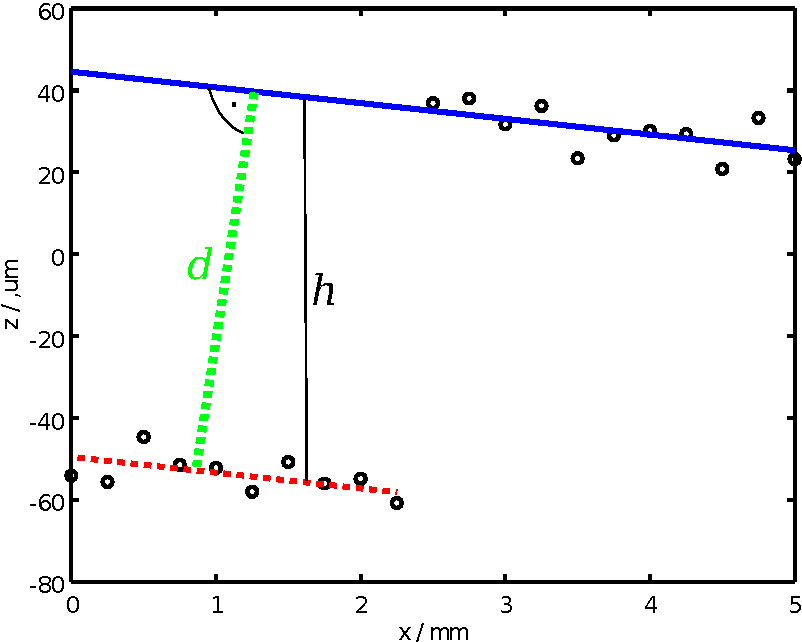
\includegraphics[width=90mm]{02_vorlesung/media/uebungA5_step_plot.pdf}
\end{center}

%\vspace{2mm}

\begin{tabular}{l|c|c|c|c|c|c|c|c|c|c}
	\hline
	$x / \mathrm{mm}$ &
	0.00 & 0.25 & 0.50 & 0.75 & 1.00 & 1.25 & 1.50 & 1.75 & 2.00 & 2.25 \\
	\hline
	$z / \mathrm{\mu m}$ &
	-54.08 &-55.63 &-44.65 &-51.44 &-52.21 &-58.01 &-50.76 &-56.01 &-54.86 &-60.77\\ 
	\hline
\end{tabular}

\vspace{2mm}

\begin{tabular}{l|c|c|c|c|c|c|c|c|c|c|c}
	\hline
	$x / \mathrm{mm}$  & 2.50 &
	2.75 & 3.00 & 3.25 & 3.50 & 3.75 & 4.00 & 4.25 & 4.50 & 4.75 & 5.00 \\
	\hline
	$z / \mathrm{\mu m}$ &36.85 &38.02 &31.71 &36.21 &23.39 &29.01 &30.11 &29.35 &20.81 &33.27 &23.19\\
	\hline
\end{tabular}

\vspace{2mm}

Die Modellgleichung, mit der die Stufe beschrieben wird, ist
$$
z_j \; = \; a \, x_j \, + \, c \, + \, h \, \delta_{j \in C} \; + \; \varepsilon_j
$$
mit $C$ Menge der Indizes von 1 bis $J_C$. Hier sei $J_C = 10$:
$$
C \; = \; \{\, j \, | \, j = 1, 2, \dots, J_C \}
$$
und
$$
\delta_{j \in C} \; = \; \left\{
\begin{array}{ll}
1 & \mathrm{falls} \; \;  j \in C \; \mathrm{~d.h.~} j = 1 \; \mathrm{~oder} \; j = 2
\mathrm{~oder} \; \dots \; j = J_C\\
0 & \mathrm{sonst}
\end{array} \right.
$$
Dabei ist $h$ noch nicht die Stufenhöhe, sondern deren Projektion auf die vertikale Achse.
Die Stufenhöhe $d$ ist der senkrechte Abstand zwischen den beiden parallelen Geraden, die jeweils durch die Punkte auf dem oberen und dem unteren Niveau gehen.

\begin{itemize}
	\item[a)] Stellen Sie das lineare Gleichungssystem auf, das sich durch partielles Ableiten
	für das Optimierungsproblem
	$$
	\min\limits_{a,c,h} \left\{\sum_{j=1}^{J_T} \varepsilon_j^2\right\}
	$$
	ergibt, mit $J_T = 21$.
	\item[b)] Schreiben Sie die Gleichung für die Stufenhöhe $d$ als Funktion von $h$ und $a$ auf.
	\item[c)] Schreiben Sie die Gleichung für die Varianz der Residuen auf.
	\item[d)] Schreiben Sie die Formel für die Kovarianzmatrix der Modellparameter
	$a, c, h$ auf.
	\item[e)] Verwenden Sie eine Programmierumgebung Ihrer Wahl, Matlab, Octave, Python, R, ...
	die Ihnen einen Solver für lineare Gleichungssysteme zur Verfügung stellt, sowie
	eine Routine zur Matrixinversion und berechen Sie die Zahlenwerte für die Modellparameter
	sowie deren Kovarianzmatrix.
\end{itemize}
Anmerkung: Die inverse Matrix brauchen Sie nicht analytisch zu berechnen, sondern
	lediglich $(...)^{-1}$ zu notieren


\subsection{2. Aufg zur Linearen Regression}
\label{Vorl2Regressionsaufg2}

Gegeben sind 5 Messpunkte
\begin{table}[htb!]
	\centering
	\begin{tabular}{l|c c c c c c}
		$X_i$ & 1 & 2 & 3 & 4 & 5 \\ \hline
		$Y_i$ & 0.4 & 0.55 & 0.70 & 0.75 & 0.8
	\end{tabular}
\end{table}
\begin{itemize}
	\item [(a)] Führen Sie eine lineare Regression durch, indem
	Sie den y-Abschnitt $\hat\theta_0$ und die Steigung $\hat\theta_1$ bestimmen. Geben Sie das Bestimmtheitsmaß $\rho_{XY}^2$ an.
	\item[(b)] Bestimmen Sie die Residuen $\varepsilon_j$ und das 
	Qualitätsmaß $Q(\hat\theta _0,\hat\theta _1)$ der Regression. Geben Sie die Varianz der Residuen 
	$s^2(\hat\theta_0,\hat{\theta_1})$ an?
	\item[(c)] Geben Sie den Standardabweichung (standard error) der beiden 
	Regressionsparameter $\hat\theta_0$ und $\hat\theta_1$ an?
	
	% Geben Sie das 95\%ige Vertrauensintervall
	% von	$\hat\theta_0$ und $\hat\theta_1$ an.
% 	Es wird dazu das t-Quantil für 3 Freiheitsgrade (5 Messpunkte minus
%	2 Parameter = 3 Freiheitsgrade) benötigt.
%	Das t-Quantil für den beidseitigen Vertrauensbereich von 95\%
%	für 3 Freiheitsgrade ist gegeben durch $t_3=3.1824$. 
%		\newline
%	Man erhält das t-Quantil durch den Matlab/Octave-Befehl: \texttt{tinv(0.975,3) = 3.31824} (\texttt{tinv} berechnet den einseitigen Vertrauensbereich)
%	oder man schlägt in einem Tabellenwerk nach;
%	siehe z.~B. https://de.wikipedia.org/wiki/Studentsche\_t-Verteilung
\end{itemize}




%
\chapter{Optimierung nichtlinearer Modelle}

\section{Konzepte von Optimierungsverfahren für nichtlineare Modelle}
Während dieser Vorlesungsreihe beleuchten wir die Thematik physikalische Größen zu ermitteln, die
indirekt zugänglich sind. Sie werden über eine Modellbildung als Modellparameter approximiert.
In den bisherigen Kapiteln hatten wir uns damit befasst, Modellparameter linearer Modelle, zu schätzen.
Die Besonderheit dabei ist, dass die \textsl{Kostenfunktion} $Q$ eine lineare Abhängigkeit von den
Modellparametern hat, so dass die Modellparameter
im Fall der Ausgleichsrechnung nach der Methode der kleinsten Quadrate durch Lösen eines 
linearen Gleichungssystems ermittelt werden können.
Im vorangegangen Kapitel wurde in Gl.~(\ref{linRegGleichungssystem}), Gl.~(\ref{GleichungssytemKostenfkt})
 und Gl.~(\ref{LsgRegressionGlSys}) gezeigt, dass das Gleichungssystem
aufgestellt wird, indem der Gradient, der die Kostenfunktion nach den Modellparametern ableitet, gleich Null
gesetzt wird, um das Maximum zu finden.

Für den Fall, dass die Modellparameter nicht linear in die Kostenfunktion $Q$,
auch \textsl{Zielfunktional} genannt, eingehen,
erfolgt die Schätzung der Modellparameter durch Variation, also durch Optimierung derart, um
das Minimum der Optimierungszielfunktion $Q$ zu finden.

Wir sind von normalverteilten Abweichungen ausgegangen und haben uns
die Likelihoodverteilungen angeschaut. Als Beispiel nehmen wir ein Modell mit 2 Parametern, bei
dem eine Gerade durch den Ursprung des Koordinatensystems eines dreidimensionalen
Raums gehe und bei dem alle drei Achsen von der gleichen physikalischen Dimension seien.
Die beiden zu schätzenden Parameter seien hier der Azimutalwinkel $\alpha$ und der 
Polarwinkel $\theta$, die die gesuchte Richtung der Geraden beschreiben.
Ein Punkt $\mathbf{r}$, der exakt auf der Geraden liegt, erfülle
\begin{equation}
\mathbf{r} \; = \; \lambda \mathbf{u} \qquad \mathrm{mit} \qquad
\mathbf{u}(\alpha,\theta) \; = \; \left(\begin{array}{c}
\cos(\alpha) \sin(\theta)\\
\sin(\alpha) \sin(\theta)\\
\cos(\theta) \end{array}\right) \qquad \mathrm{und} \qquad \lambda \in I \!\! R.
\end{equation}
\begin{figure}
\begin{center}
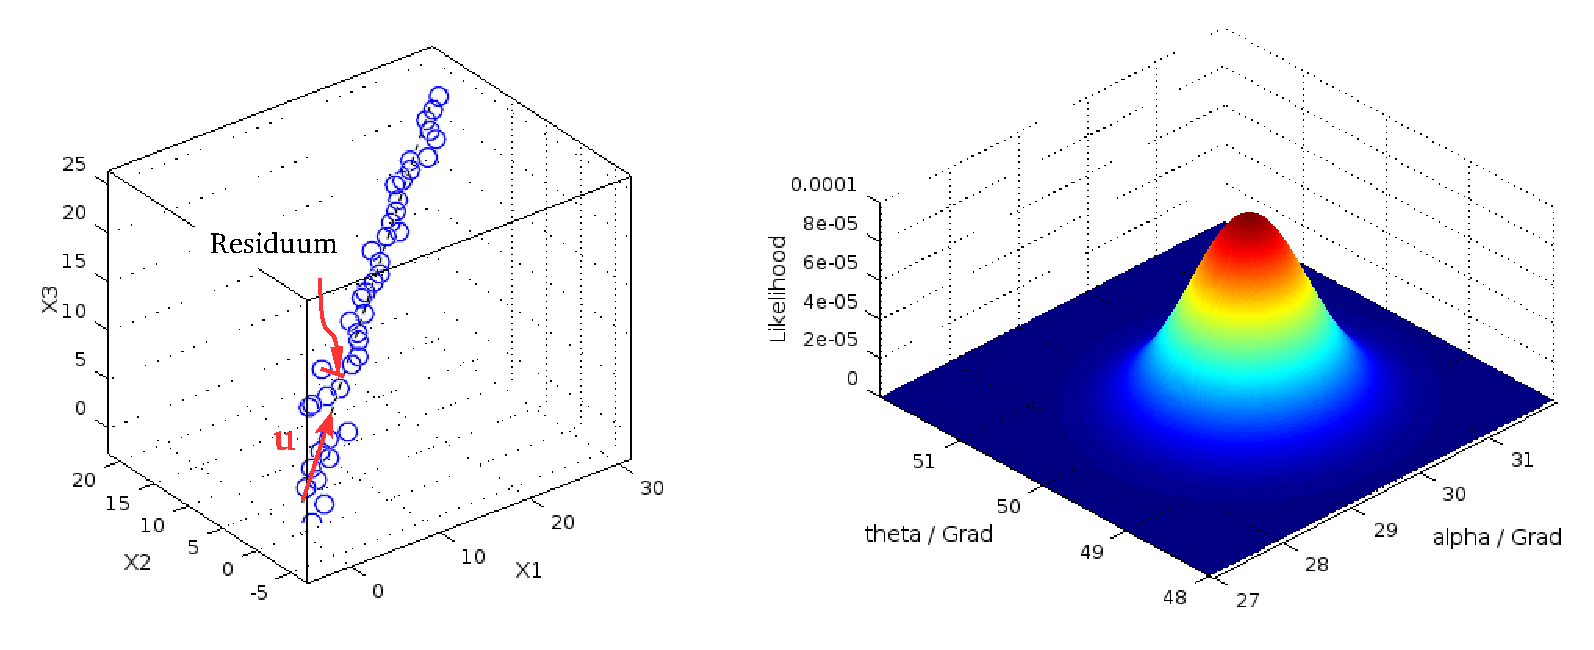
\includegraphics[width=0.95\textwidth, angle = 0]{03_vorlesung/media/LSopti_example1.pdf}
\end{center}
\caption{Modell mit 2 zu schätzenden Parametern (\textsl{links}) und der dazugehörigen
Likelihood für normalverteilte Residuen (\textsl{rechts}).\label{LSoptiExample1}}
\end{figure}

Abb.~\ref{LSoptiExample1} zeigt das Modell als schwarz gestrichelte Gerade und die Beobachtungen als blaue Kreise, sowie rechts die Likelihoodverteilung. Wir hatten bereits ausführlich darüber gesprochen, dass die Suche des Maximums der Likelihood in die Suche des Minimums übergeht. Es gelte nun diejenige Geradenrichtung zu finden, für die die senkrechten Abstände,
die Residuen $\varepsilon_j$,  der beobachteten Punkte (Messpunkte) $\mathbf{r}_{\mathrm{Mess},j} = (X_{1,j}, X_{2,j}, X_{3,j})^\mathsf{T}$ minimal sind. Für das Kriterium für minimale Abstände, also die Kostenfunktion $Q$, setzen wir wieder voraus, dass die Messpunkte gaußverteilt um eine Gerade streuen. Den Betrag für die senkrechten Abstände berechnen wir mit
\begin{equation}
\varepsilon(\alpha,\theta)_j \; = \; \left| \mathbf{r}_{\mathrm{Mess},j} \; - \;
( \mathbf{r}_{\mathrm{Mess},j} \cdot \mathbf{u}(\alpha,\theta) ) \, \mathbf{u}(\alpha,\theta) \right|
\end{equation}
mit $|$ als Betrag gemäß $| \mathrm{a} | = \sqrt{a_1^2 + a_2^2 + a_3^2}$.
Für die Likelihoodverteilung auf der rechten Seite von Abb.~\ref{LSoptiExample1} verwenden wir
die Wahrscheinlichkeitsdichte gemäß
\begin{equation}
p(\varepsilon_1,\dots,\varepsilon_J | \alpha, \theta)
\propto e^{-\frac{1}{2} \, \sum\limits_{j=1}^J \, \left(\frac{\varepsilon(\alpha,\theta)_j}{\sigma} \right)^2} .
\end{equation}
Für den Schätzvorgang wählen wir wieder für das Zielfunktional $Q$ die Summe der Quadrate der Residuen $Q = \sum \varepsilon_j^2$,
also einen Optimierungsvorgang gemäß der Methode der kleinsten
Residuenquadratsumme (RQS).
\begin{equation}
\min_{\alpha,\theta} \, \sum\limits_{j=1}^J \, \varepsilon(\alpha,\theta)_j^2 .
\end{equation}
Die Optimierungsrechnung bietet sehr unterschiedliche Methoden für eine Minimumsuche.

Wir können sie grob danach einteilen
\begin{itemize}
\item ob das nächste Modellparametertupel gemäß einer gewissen Strategie aus
mehreren Vor\-gänger\-tupeln mit den dazugehörigen Werten der Kostenfunktion $Q$ gewonnen wird
\item oder ob nicht nur die Kostenfunktion $Q$ direkt, sondern auch deren Gradienten bestimmt
werden.
\end{itemize}
Ein möglicher, vielfach genutzer Ansatz für das Verwenden mehrerer Vorgängertupel mit den dazugehörigen Werten der RQS
ist die Simplexmethode nach Nelder und Mead aus dem Jahr 1965. Er wird als Bibliotheksfunktion \texttt{fmins}
in Matlab und Gnu-Octave zur Verfügung gestellt. Mit Simplex ist ein Vieleck gemeint, das $M+1$ Ecken hat für $M$
Parameter, in unserem Beispiel also drei Ecken für zwei Parameter, was in Abb.~\ref{LSoptiExample1NM} durch
schwarz umrandete weiße Punkte, die mit schwarzen, durchgezogenen Linien verbunden sind, skizziert ist. Zum Aufbau eines
Startsimplex wird ein Startwerttupel $\mathbf{p}_{0,0}$ des Modellparametervektors gewählt und zu jedem Parameter ein
weiterer Vektor, der eine Variation $\Delta P_m$ repräsentiert:
\begin{equation}
\mathbf{p}_{0,1} \; = \; \mathbf{p}_{0,0} \; + \; \left(\begin{array}{c}
\Delta P_1 \\
0 \\
\vdots \\
0
\end{array}\right) \qquad
\mathbf{p}_{0,m} \; = \; \mathbf{p}_{0,0} \; + \; \left(\begin{array}{c}
0 \\
\vdots \\
0 \\
\Delta P_m \\
0 \\
\vdots \\
0
\end{array}\right) \qquad
\mathbf{p}_{0,M} \; = \; \mathbf{p}_{0,0} \; + \; \left(\begin{array}{c}
0 \\
\vdots \\
0 \\
\Delta P_M
\end{array}\right)
\end{equation}
\begin{figure}
\begin{center}
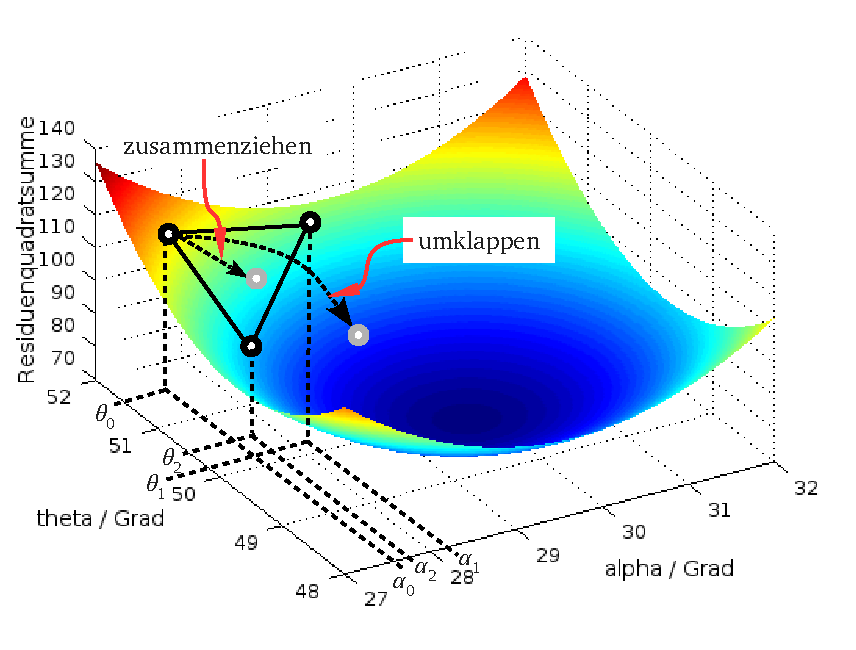
\includegraphics[width=0.6\textwidth, angle = 0]{03_vorlesung/media/LSopti_example1_LS_NM.pdf}
\end{center}
\caption{Residuenquadratsumme des Beispielmodells mit 2 zu schätzenden Parametern
und Simplex für Optimierungsverfahren nach Nelder und Mead.\label{LSoptiExample1NM}}
\end{figure}

Die Strategie ist es, diesen Simplex durch Zusammenziehen oder durch Umklappen dazu zu bewegen, in
die Minimumsmulde herunter zu klettern, was in Abb.~\ref{LSoptiExample1NM} durch hellgrau umrandete
weiße Punkte und durch Pfeile skizziert ist. Die Entscheidung, wann er sich zusammen zieht und dadurch
auch verkleinert und wann er umklappt und wann er notfalls auch wieder gestreckt (vergrößert) werden
muss wird anhand dessen getroffen, ob die Werte des Zielfunktionals $Q$ kleiner werden oder nicht.
Wenn er klein und flach im Tal angekommen ist, terminiert der Algorithmus. Hierzu gibt es dann noch
verschiedene Ansätze, wie überprüft wird, ob er zu weit über dem Tal waagerecht festhakt und eigentlich
noch eine zu große Mulde darunter liegt und eines der Simplexbeine angezogen werden muss.

Dieses Verfahren eignet sich auch für zu minimierende Zielfunktionale, die nicht so schön stetig
differenzierbar, d.h.\ glatt, in der Talmulde sind. Für Messungen mit Beobachtungen, die nicht gaußverteilt
streuen, sondern stark abweichende Punkte aufweisen, greift man auf andere Verteilungen zurück.
Eine mögliche Verteilung kann die Laplaceverteilung sein
\begin{equation}
p(\varepsilon_1,\dots,\varepsilon_J | \alpha, \theta)
\propto e^{-\frac{1}{2} \, \sum\limits_{j=1}^J \, \frac{| \varepsilon(\alpha,\theta)_j |}{\sigma} } 
\end{equation}
was bedeutet, dass sie eine Exponentialverteilung der Absolutbeträge der
Residuen ist. Bei dem zu minimierenden Exponenten
\begin{equation}
\min_{\alpha,\theta} \, \sum\limits_{j=1}^J \, | \varepsilon(\alpha,\theta)_j |
\end{equation}
bildet sich die Minimumsmulde durch die Betragsbildung zu einer ausgeprägt scharfen Spitze aus.
Im Minimum gibt es also keine einheitliche Steigung. Je nach Richtung, von der man sich ihr nähert,
gibt es sehr unterschiedliche Steigungen, was soviel bedeutet wie die Nichtstetigkeit der
Steigungsfunktion. Steigungen im mehrdimensionalen Raum heißen Gradienten. Die Gradientenfunktion
ist nicht stetig, die Funktion selber also nicht stetig differenzierbar. Für das Simplexverfahren
spielt dies aber keine Rolle. Das Simplexverfahren hat aber den Nachteil, dass es sehr 
empfindlich darauf reagiert, welchen Startsimplex man zu Beginn auswählt. Es kann dadurch
im harmlosen Fall relativ langsam werden, aber im ungünstigsten Fall in die Irre laufen und gar
nicht konvergieren. Auch kann das Problem des Festhakens bei Optimierungsaufgaben mit vielen
Parametern zu einem schwerwiegenderen werden.

\begin{figure}
\begin{center}
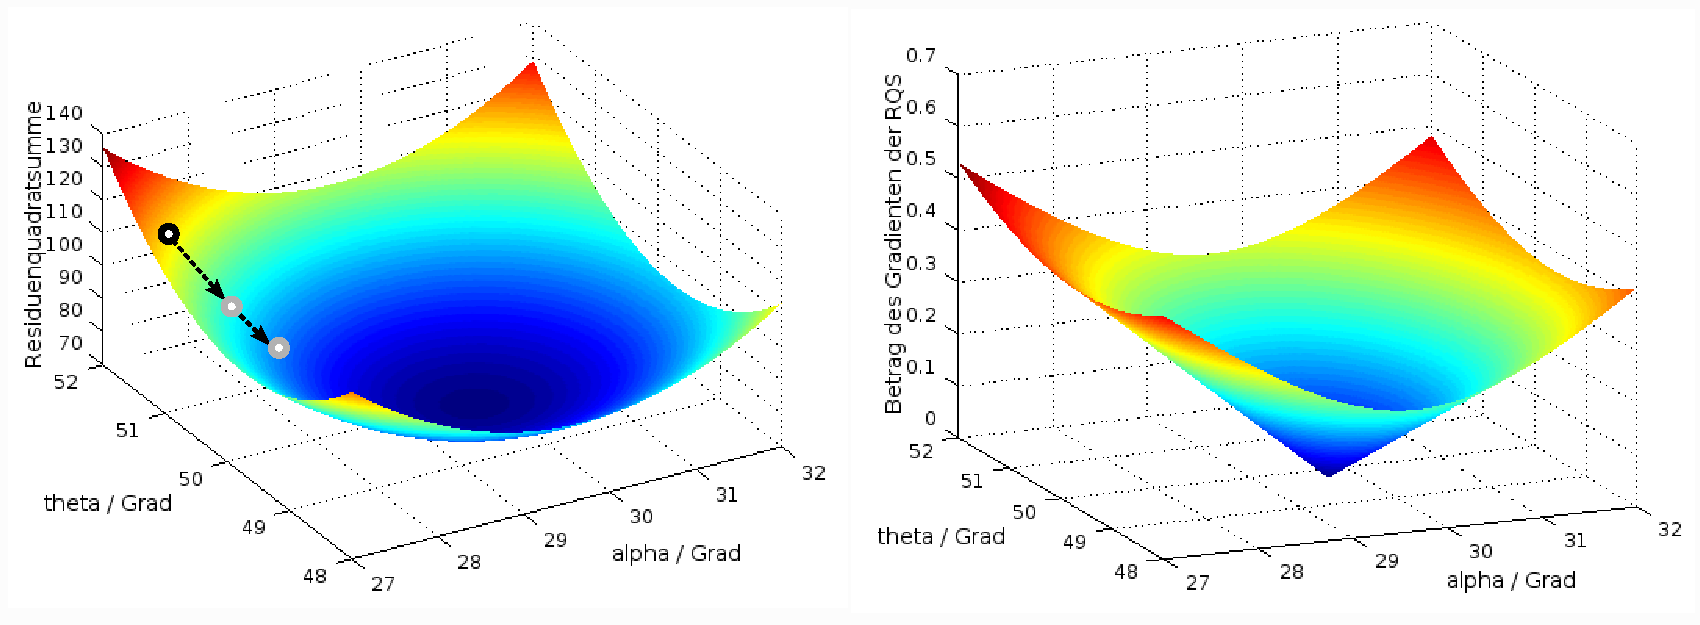
\includegraphics[width=0.95\textwidth, angle = 0]{03_vorlesung/media/LSopti_example1_LS_Grad.pdf}
\end{center}
\caption{Residuenquadratsumme des Beispielmodells mit 2 zu schätzenden Parametern
und Gradienten eingezeichnet als Pfeile (\textsl{links}) und Beträge der
Gradienten als Funktion der 2 zu schätzenden Parameter (\textsl{rechts}).\label{LSoptiExample1Grad}}
\end{figure}
Für zu minimierende Zielfunktionale wie wir sie bei normalverteilten Residuen, also bei
den rundlichen, stetig differenzierbaren Kostenfunktionen als Residuenquadratsummen haben, können wir Verfahren
einsetzen, die nicht nur die Kostenfunktion $Q$ direkt, sondern auch deren Gradienten $\nabla Q$ verwenden.
Hierzu wird \textsl{ein} Startwertetupel (nicht wie bei der Simplexmethode $M+1$)
für die Modellparameter gebracht. Es wird der Gradient, also die Richtung des steilsten
Abhangs der Kostenfunktion zusammen mit dem Wert der Steigung an der Position des Startwerttupels
bestimmt. Dieses Verfahren beleuchten wir im folgenden Abschnitt anhand unseres Beispiels etwas genauer.

\section{Gradientenverfahren für nichtlineare Zielfunktionale}

Das Gradientenverfahren braucht wie alle anderen Methoden zur Schätzung von Parametern, die
nicht linear in die Residuen eingehen, ein Tupel von Startwerten der Parameter, was wir in
Abb.~\ref{LSoptiExample1Grad} als schwarz umrandeten weißen Punkt dargestellt haben.
In Abb.~\ref{LSoptiExample1Grad} ist die Idee illustriert, wie sich die Position des
Parametervektors verändert. Die Änderungsvektoren $\Delta \mathbf{p}$ werden aus der Richtung
des steilsten Abhangs ermittelt, wie durch die Pfeile mit gestrichtelter Linie skizziert. 
Der Gradient des Betrags eines Residuums an der Stelle des Startwertevektors $(\alpha_0, \theta_0)$
ist der Vektor der partiellen Ableitungen
\begin{equation}
\left. \nabla_{\alpha,\theta} \varepsilon_j \right|_{\alpha_0, \theta_0} \; = \;
\left(\begin{array}{c}
\frac{\partial}{\partial \alpha} \\
\frac{\partial}{\partial \theta}
\end{array}\right) \left. \varepsilon_j \right|_{\alpha_0, \theta_0} .
\end{equation}
Das auf die Spitze gestellte Dreieck heißt Nablaoperator.
Die Schreibweise $|_{\alpha_0, \theta_0}$ lesen wir \glqq an der Stelle\grqq ~$(\alpha_0, \theta_0)$.
Für die Minimierung bestimmen wir die Stelle $(\hat \alpha, \hat \theta)$, an der sich die Talsohle
der Mulde der RQS-Funktion befinden. Anders gesagt suchen wir die Position im Modellparameterraum,
die unten in der Mulde RQS-Funktion liegt,
in der keine Steigung mehr vorhanden ist, d.h.\ der Gradient ein Nullvektor ist, d.h.
\begin{equation}
\lim_{\alpha \rightarrow \hat \alpha, \theta \rightarrow \hat \theta} 
\left\{\nabla_{\alpha,\theta} \,
\sum\limits_{j=1}^J \, \varepsilon(\alpha,\theta)_j^2
\right\} \; = \; 
\left(\begin{array}{c}
0 \\
0
\end{array}\right) .
\label{LSschaetzung1}
\end{equation}
Hierbei müssen wir uns aber darüber im Klaren sein, dass Gradient gleich Nullvektor nicht nur
bei einem Minimum vorliegt, sondern auch bei einem Maximum und bei einem Sattelpunkt, weshalb wir
im letzten Abschnitt ein Verfahren kurz vorstellen, das sich mit dieser Problematik besser
auseinander setzt.

Wir ziehen den Nablaoperator in die Summe rein und
verwenden die Kettenregel, äußere Ableitung mal innere Ableitung:
\begin{equation}
\nabla_{\alpha,\theta} \,
\sum\limits_{j=1}^J \, \varepsilon(\alpha,\theta)_j^2
 \; = \; 
\sum\limits_{j=1}^J \, \nabla_{\alpha,\theta} \, \varepsilon(\alpha,\theta)_j^2
 \; = \; 
2 \, \sum\limits_{j=1}^J \, \varepsilon(\alpha,\theta)_j \nabla_{\alpha,\theta} \, \varepsilon(\alpha,\theta)_j
 \; \overset{!}{=} \; 
\left(\begin{array}{c}
0 \\
0
\end{array}\right) .
\label{GradientQ2params}
\end{equation}

Die beiden Parameter $\alpha,\theta$ fassen wir zusammen in einen Parametervektor $\mathbf{p}$ und
betrachten im folgenden den Allgemeinfall für $M$ Parameter $\mathbf{p} = (P_1,\dots,P_M)^\mathsf{T}$.
Die Residuen sind dann jeweils Funktion des Parametervektors
$\boldsymbol \varepsilon(\mathbf{p}) = (\varepsilon_1(\mathbf{p}), \dots, \varepsilon_J(\mathbf{p}))^\mathsf{T}$,
so dass die Kostenfunktion $Q$ entsprechend Funktion des Parametervektors ist
\begin{equation}
Q(\mathbf{p}) \; = \; \boldsymbol \varepsilon^\mathsf{T}(\mathbf{p}) \, \boldsymbol \varepsilon(\mathbf{p}),
\label{Zielfunktional}
\end{equation}
für die wir das Minimum suchen mit
\begin{equation}
\min_{\mathbf{p}} \left\{ Q(\mathbf{p}) \right\}
\end{equation}
indem wir nach dem Nullstellenvektor der Gradientenfunktion
\begin{equation}
\nabla_{\mathbf{p}} Q(\mathbf{p}) \; = \;
 2 \, \boldsymbol \varepsilon^\mathsf{T} \, \left( \nabla_{\mathbf{p}}^\mathsf{T} \boldsymbol \varepsilon \right)
\label{ZielfunktionalGrad}
\end{equation}
suchen, für den $Q$ ein Minimum und nicht ein Maximum oder Sattelpunkt annimmt.
Dabei ist $\nabla_{\mathbf{p}}$ Spaltenvektor und $\nabla_{\mathbf{p}}^\mathsf{T}$ Zeilenvektor
mit den partiellen Ableitungsoperatoren $\frac{\partial}{\partial P_m}$.
Wir suchen dasjenige $\mathbf{p}$ für das
\begin{equation}
\lim_{\mathbf{p} \rightarrow \mathbf{\hat p}}
\nabla_{\mathbf{p}} Q(\mathbf{p}) \; = \; \left(\begin{array}{c} 0\\ \vdots \\ 0 \end{array}\right)
\label{ZielfunktionalGrad1}
\end{equation}
Bei der Suche nach dem Minimum wird mit einem Tupel von Parametern angefangen, also
mit einem Startwertvektor $\mathbf{p}_0$. Dann wird ein Schrittvektor $\Delta \mathbf{p}_0$ ermittelt,
der gegangen wird, um
zu einem Nachfolgepunkt im Raum der Modellparamter zu gelangen $\mathbf{p}_1 = \mathbf{p}_0 + \Delta \mathbf{p}_0$.
Dies erfolgt solange, bis der Parametervektor beliebig dicht an das Minimum von $Q$ gelangt sind. Es gibt damit eine
gewisse Anzahl $K$ von Iterationschritten, derart dass der Vektor $\mathbf{p}_K = \mathbf{\hat p}$ für minimales
$Q$ als Tupel von Schätzwerten für die Modellparameter verwendet wird.
Die einzelnen Iterationsschritte $\kappa$ bedeuten eine Revision des Modellparametervektors
\begin{equation}
\mathbf{p}_\kappa = \mathbf{p}_{\kappa-1} + \Delta \mathbf{p}_{\kappa-1}
\label{Revisionsschritt}
\end{equation}
mittels \textsl{Inkrementvektoren}
$\Delta \mathbf{p}_1, \dots, \Delta \mathbf{p}_{\kappa}, \dots, \Delta \mathbf{p}_{K-1}$.

Wir nehmen eine Taylorreihenentwicklung vor, über die wir die Gradientenfunktion des Zielfunktionals
als lineare Funktion eines \textsl{Inkrementvektors} $\Delta \mathbf{p}$ darstellen. Dazu entwickeln
wir die Residuen $\varepsilon_j$ in Taylorreihe bis zum linearen Term
\begin{equation}
\left(\begin{array}{c}
\varepsilon_1(\mathbf{p}) \\
\vdots \\
\varepsilon_j(\mathbf{p}) \\
\vdots \\
\varepsilon_J(\mathbf{p}) 
\end{array}\right)
\; = \; 
\left(\begin{array}{c}
\varepsilon_1(\mathbf{p}_\kappa) \; + \; \nabla_{\mathbf{p}} \left. \varepsilon_1 \right|_{\mathbf{p}_\kappa} \cdot \Delta \mathbf{p}\\
\vdots \\
\varepsilon_j(\mathbf{p}_\kappa) \; + \; \nabla_{\mathbf{p}} \left. \varepsilon_j \right|_{\mathbf{p}_\kappa} \cdot \Delta \mathbf{p}\\
\vdots \\
\varepsilon_J(\mathbf{p}_\kappa) \; + \; \nabla_{\mathbf{p}} \left. \varepsilon_J \right|_{\mathbf{p}_\kappa} \cdot \Delta \mathbf{p}
\end{array}\right).
\label{TaylorResi1}
\end{equation}
Hier bilden die partiellen Ableitungen der einzelnen Residuen nach allen Parametern eine $J \times M$-Matrix, die \textsl{Jakobimatrix}
genannt wird:
\begin{equation}
\boldsymbol{J}^{(\kappa)} \; = \; \left(\begin{array}{ccc}
\left. \frac{\partial \varepsilon_1}{\partial P_1} \right|_{\mathbf{p}_\kappa} & \dots & \left. \frac{\partial \varepsilon_1}{\partial P_M} \right|_{\mathbf{p}_\kappa} \\
 & \ddots & \\
\left. \frac{\partial \varepsilon_J}{\partial P_1}\right|_{\mathbf{p}_\kappa} & \dots & \left. \frac{\partial \varepsilon_J}{\partial P_M}\right|_{\mathbf{p}_\kappa}
\end{array}\right) ,\; \textrm{bzw.} \; J_{jm}^{(\kappa)}= \left. \frac{\partial \epsilon_j}{\partial p_m}\right|_{\mathbf{p}_\kappa}
\;\textrm{mit} \; j=1\ldots J; \;\; m=1\ldots M.
\end{equation}
Der hochgestellte und in Klammern gesetzte Index $\kappa$ 
an dem Symbol für die \textsl{Jacobimatrix}, soll bedeuten,
dass dies die \textsl{Jacobimatrix} für den Parametervektor an der Stelle
$\mathbf{p}_\kappa$ ist, also für die Position der Modellparameter beim $\kappa$-ten Interationsschritt.
Der Begriff Jacobimatrix bedeutet nur, dass es
sich um eine Matrix partieller Ableitungen handelt.
\begin{quote}
Die \textsl{Jacobimatrix} (benannt nach Carl Gustav Jacob Jacobi; auch 
\textsl{Funktionalmatrix}, \textsl{Ableitungsmatrix} oder \textsl{Jacobische} genannt)
einer differenzierbaren Funktion
$f\colon I \! \! R^{n} \mapsto I \! \! R ^{m}$ ist die 
$m\times n$-Matrix sämtlicher erster partieller Ableitungen.
\end{quote}


Einsetzen dieser Jacobimatrix in Gl.~(\ref{TaylorResi1}) liefert dann
\begin{equation}
\left(\begin{array}{c}
\varepsilon_1(\mathbf{p}) \\
\vdots \\
\varepsilon_J(\mathbf{p}) 
\end{array}\right)
\; = \; 
\left(\begin{array}{c}
\varepsilon_1(\mathbf{p}_\kappa) \\
\vdots \\
\varepsilon_J(\mathbf{p}_\kappa)
\end{array}\right)
\; + \; \boldsymbol{J}^{(\kappa)} \Delta \mathbf{p} .
\label{TaylorResi2}
\end{equation}
Wir schreiben Gl.~(\ref{TaylorResi2}) in Vektorschreibweise, mit $\boldsymbol{\varepsilon}$ hier als Spaltenvektor
der einzelnen Residuen.
\begin{equation}
\boldsymbol{\varepsilon}(\mathbf{p})
\; = \; 
\boldsymbol{\varepsilon}(\mathbf{p}_\kappa)
\; + \; \boldsymbol{J}^{(\kappa)} \Delta \mathbf{p} .
\label{TaylorResi3}
\end{equation}
Ferner setzen wir die Jacobimatrix in Gl.~(\ref{ZielfunktionalGrad}) ein
\begin{equation}
\frac{1}{2} \nabla_{\mathbf{p}} Q(\mathbf{p})  \; = \; \boldsymbol{\varepsilon}^\textsf{T}(\mathbf{p})
 \, \boldsymbol{J}
\label{ZielfunktionalGradJ}
\end{equation}
% \; \overset{!}{=} \; \left(\begin{array}{c} 0\\ \vdots \\ 0 \end{array}\right)
% \label{GradientQv}
Wir setzen die Reihenentwicklung der Residuen Gl.~(\ref{TaylorResi3}) ein und 
den Gradienten Gl.~(\ref{ZielfunktionalGradJ}) in Gl.~(\ref{ZielfunktionalGrad1}) ein.
So erhalten wir ein in $\Delta \mathbf{p}$ lineares Gleichungssystem:
\begin{equation}
\left( \boldsymbol{\varepsilon}(\mathbf{p}_\kappa)
\; + \; \boldsymbol{J}^{(\kappa)} \Delta \mathbf{p}_\kappa \right)^\textsf{T} \, \boldsymbol{J}^{(\kappa)}
\; \overset{!}{=} \; \left( 0 \dots  0 \right)
\label{GradientQlinGl1}
\end{equation}
wobei hier der Nullvektor wie der transponierte Modellparametervektor ein
Zeilenvektor im $I \! \! R^{M}$ ist.
Wir formen diese Gleichung, die in Zeilenvektorschreibweise ist, um in
\begin{equation}
\left( \boldsymbol{J}^{(\kappa)} \Delta \mathbf{p}_\kappa \right)^\textsf{T} \, \boldsymbol{J}^{(\kappa)}
\; \overset{!}{=} \; 
- \boldsymbol{\varepsilon}(\mathbf{p}_\kappa)^\textsf{T} \, \boldsymbol{J}^{(\kappa)}
\label{GradientQlinGl2}
\end{equation}
und transponieren diese, um sie als lineares Gleichungssytem mit Spaltenvektoren vorliegen zu haben
d.h.
\begin{equation}
 \boldsymbol{J}^{(\kappa) \textsf{T}} \, \boldsymbol{J}^{(\kappa)} \, \Delta \mathbf{p}_\kappa
\; \overset{!}{=} \; 
-  \boldsymbol{J}^{(\kappa) \textsf{T}} \, \boldsymbol{\varepsilon}(\mathbf{p}_\kappa) .
\label{GradientQlinGl3}
\end{equation}
Die Lösung dieses linearen Gleichungssystems liefert den Inkrementvektor $\Delta \mathbf{p}_\kappa$,
mit dem wir den Schritt zur nächsten Position $\mathbf{p}_{\kappa+1} \; = \; \mathbf{p}_{\kappa} \, + \,
\Delta \mathbf{p}_{\kappa}$ gehen. Die Iterationen enden, wenn der Betrag der Gradientenfunktion oder
das Quadrat nahe Null, also kleiner als eine sehr kleine Zahl $\epsilon$ ist:
\begin{equation}
 \boldsymbol{\varepsilon}(\mathbf{p}_\kappa)^\mathsf{T}
\, \boldsymbol{J}^{(\kappa)} \, \boldsymbol{J}^{(\kappa) \textsf{T}} \, \boldsymbol{\varepsilon}(\mathbf{p}_\kappa) \;
< \; \epsilon
\end{equation}

Für Kostenfunktionen, die wie in Abb.~\ref{LSoptiExample1Grad}, ein sauber ausgeprägtes Minimum
haben, und für die ein Startwerttupel zu den Modellparametern, das nah genug an der Mulde dran ist und
sehr weit weg von irgendwelchen Maxima und Sattelpunkten, lässt sich auf diese Weise das Minimum
finden.


Um eine sinnvolle Konvergenz zu erzielen, ist eine gute Vorkenntnis, also ein geeignetes 
Modellparametertupel $\mathbf{p}_0$ erforderlich, das in einigen Problemstellungen
nur schwerlich, oder gar nicht verfügbar ist. Das bedeutet, dass nicht klar ist, ob
der Gradient dazu führt, dass der Parametervektor in eine Mulde hinab klettert, oder auf
einen Berggipfel oder entlang eines Sattelpunktes spaziert.

Die Numeriker haben Verfahren entwickelt, die auf dieser Grundidee den Gradienten
der Zielfunktion (Summe der Quadrate der Residuen) zu berechnen
basieren, aber ausgereiferter sind hinsichtlich Stabilität und Konvergenz.
Der sog.\ der \textsl{Levenberg-Marquardt}-Algorithmus ist eine solche gradientenbasierte Methode,
die in den Numerikbibliotheken zu Matlab, Gnu-Octave, Python bis hin zu Labview, für nichtlineare
Regression zur Verfügung gestellt wird. Die Grundidee dieser Methode wollen wir im Folgenden
skizzieren.

\section{Levenberg-Marquardt-Verfahren}
\begin{figure}
\begin{center}
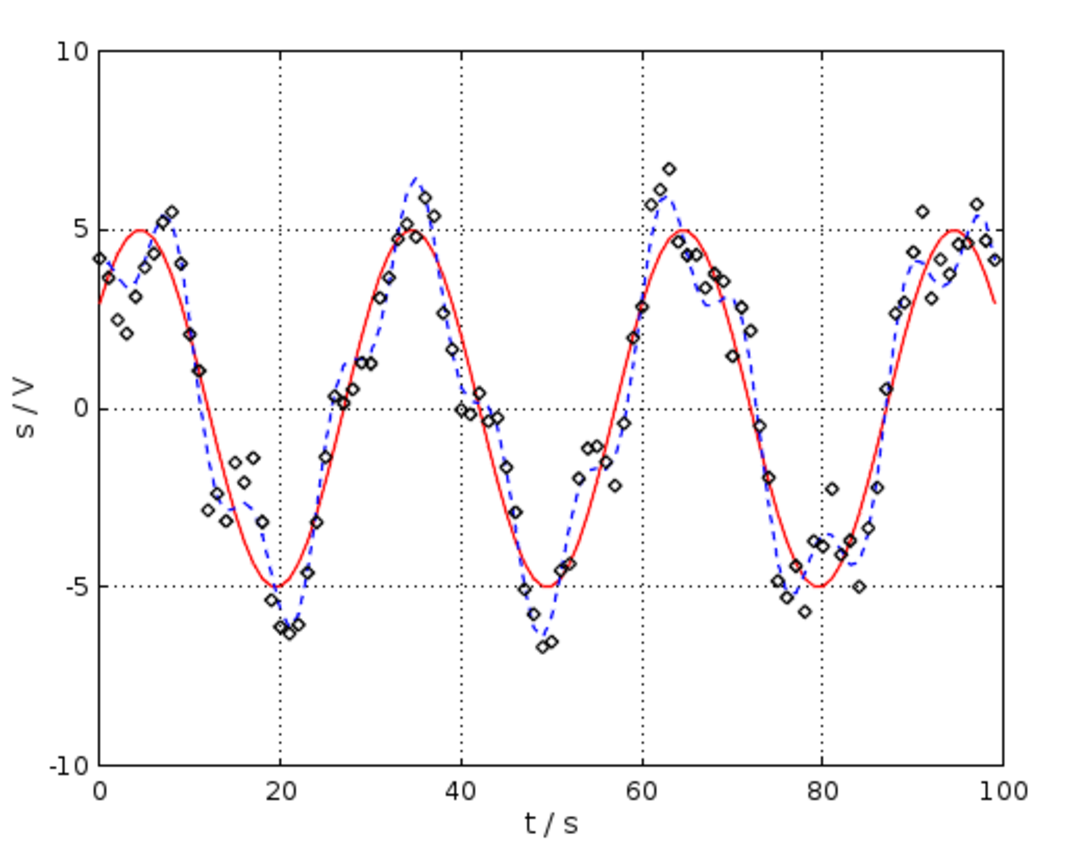
\includegraphics[width=0.6\textwidth, angle = 0]{03_vorlesung/media/pltSS_nonlin_leastsquare_sin_zB1signal.pdf}
\end{center}
\caption{Beispiel eines sinusförmigen Signals.\label{LSoptiExampleSinus}}
\end{figure}
\begin{figure}
\begin{center}
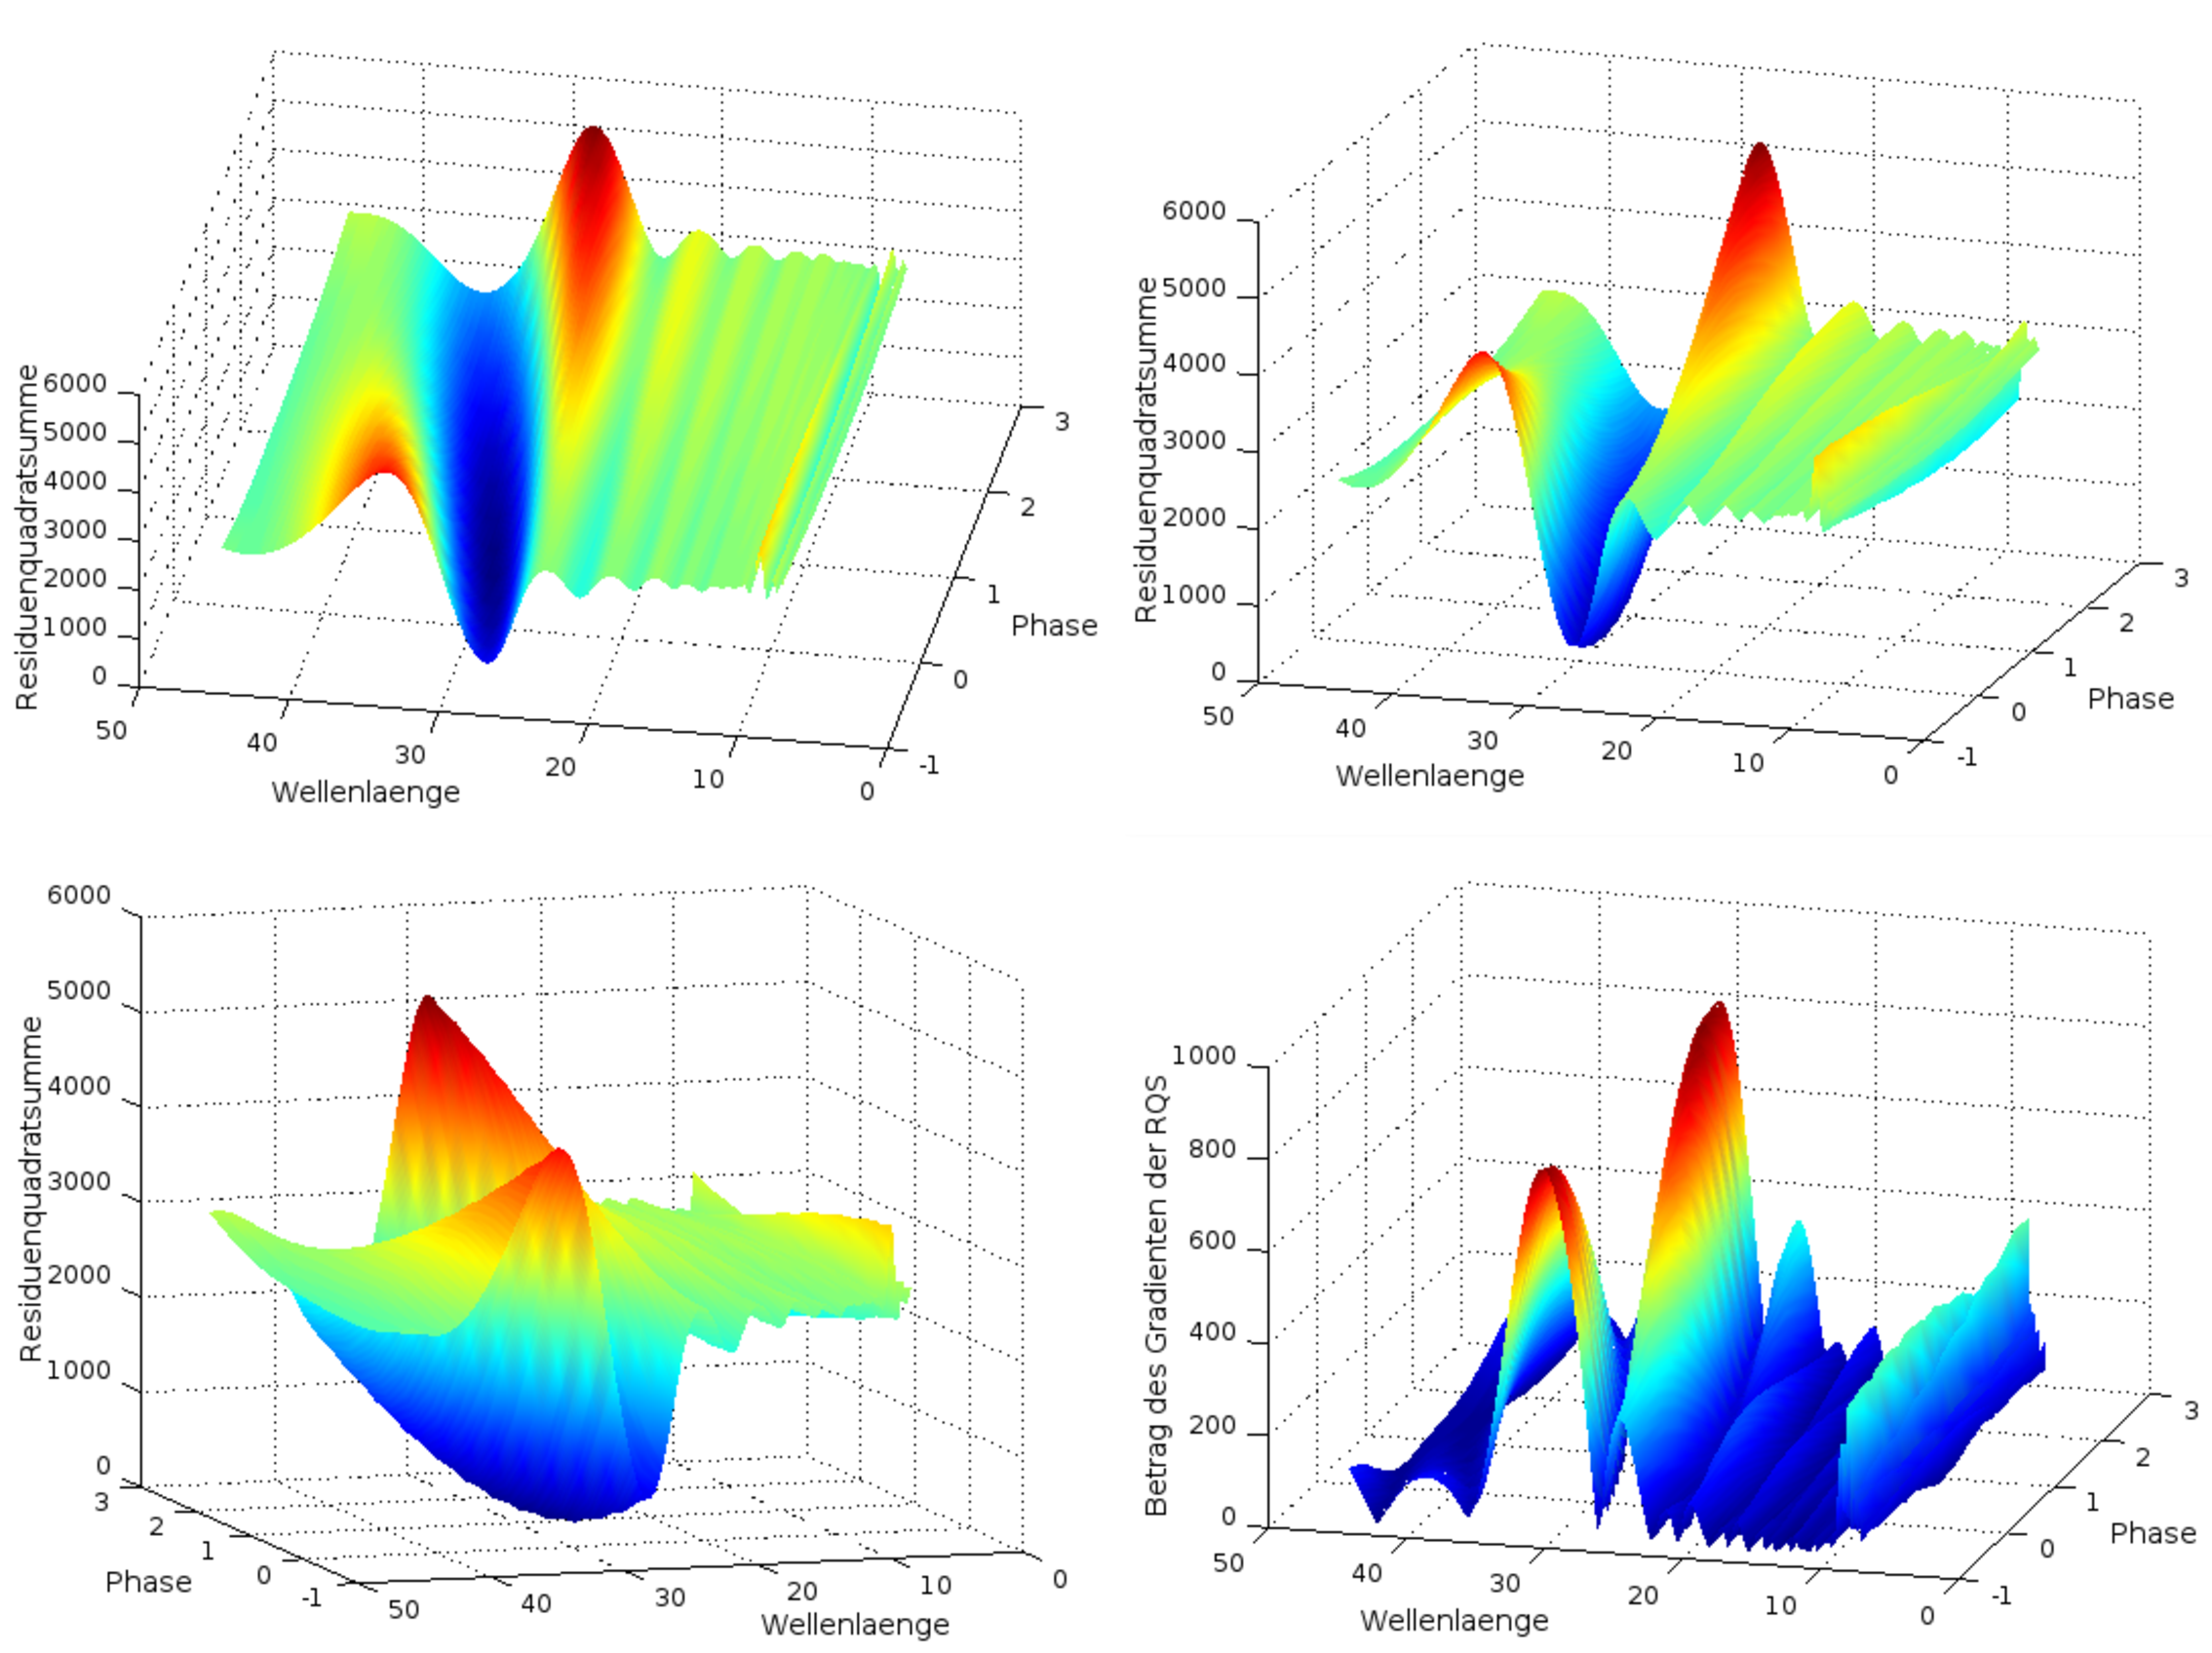
\includegraphics[width=0.9\textwidth, angle = 0]{03_vorlesung/media/pltSS_nonlin_leastsquare_sin_zB1RQS.pdf}
\end{center}
\caption{Residuenquadratsumme des Beispielmodells eines sinusförmigen Signals
in drei verschiedenen Perspektiven dargestellt (\textsl{oben} und \textsl{unten links})
 und die Beträge der
Gradienten als Funktion der 2 zu schätzenden Parameter (\textsl{unten rechts}).\label{LSoptiExample1SinusRQS}}
\end{figure}
Die Problematik, dass sich der Vektor $\Delta \mathbf{p}_{\kappa}$, den wir im
Folgenden \textsl{Inkrementvektor} nennen, verirrt und auf
einen Berggipfel oder entlang eines Sattelpunktes spaziert, soll anhand eines Beispielsignals
illustriert werden. Das Beispiel ist ein zeitabhängiges Spannungssignal mit sinusförmigem Verlauf,
dem als Störung zum einen ein Signal mit höherer Frequenz und kleinerer Amplitude aufmoduliert ist
und zum anderen ein normalverteiltes weißes Rauschen.
Die Amplitude von $5 \, V$ sei fest vorgegeben, aber die zu schätzenden Modellparameter seien
die Wellenlänge und die Phasenlage des Signals. Abb.~\ref{LSoptiExampleSinus} zeigt das Signal als
schwarze Rauten und in Rot das gesuchte \glqq wahre\grqq ~Signal und als blaue, gestrichelte Kurve
das Signal superponiert mit der höherfrequenten Modulation.

Abb.~\ref{LSoptiExample1SinusRQS} zeigt die Summe der Quadrate der Residuen RQS als
Kostenfunktion in drei verschiedenen Ansichten, die zeigen, dass es eine ausgeprägte Minimumsmulde gibt,
aber ebenso ein ausgeprägtes Maximum und noch kleine Rippeln als Nebenminima und Nebenmaxima.
Das Diagramm unten rechts zeigt die Betragsfunktion des Gradienten mit den vielen Nullstellen.
Hier sehen wir, dass sowohl die Maxima als auch die Minima die Nullstellen bilden.

Der \textsl{Levenberg-Marquardt}-Algorithmus ist ein Gradientenverfahren, bei dem das lineare
Gleichungssystems (\ref{GradientQlinGl3}) 
durch Einführen eines Dämpfungsterms erweitert wird. 

Mit der Gauss-Newton-Methode kann also passieren, dass die Summe der Residuen $Q$, siehe  nicht bei jedem Iterationsschritt kleiner
wird. Wenn jedoch der Richtungsvektor $\Delta \mathbf{p}_{\kappa}$ in die abfallende Richtung
zeigt, so kann auch nur ein Bruchteil $\alpha$ des Richtungsvektors gegangen 
werden, solange gilt:
\begin{equation}
Q(\mathbf{p}_{\kappa} + \alpha \cdot \Delta \mathbf{p}_{\kappa}) < Q(\mathbf{p}_{\kappa})
\end{equation}
D.~h., wenn bei der Gauß-Newton Methode Divergenz auftritt, so ist eine 
mögliche Verbesserung des Verfahrens, einen Bruchteil $\alpha$ des Richtungsvektors $\Delta\mathbf{p}_{\kappa}$ zu nehmen: 
\begin{equation}
\mathbf{p}_{\kappa+1}= \mathbf{p}_{\kappa} + \alpha \cdot \Delta\mathbf{p}_{\kappa}
\end{equation}
In anderen Worten, wenn der Inkrement-Vektor zu lang ist, dann muss man diesen
eben kürzen. Das geht natürlich nur unter der Voraussetzung, dass die Richtung 
des Vektors auch die Summe der Residuen weiter verkleinert. Der Bruchteil $\alpha$
liegt zwischen 
\[
0 < \alpha < 1
\] 
Wenn der optimale Bruchanteil $\alpha$ annähernd Null ist, wird eine alternative Methode zur Behandlung der Divergenz verwendet, der sog. \textbf{Levenberg-Marquardt}
Algorithmus. 
Die Normalengleichung wird modifiziert, indem der Inkrementvektor $\mathbf{p}_{\kappa}$ in Richtung des steilsten Abfalls gedreht wird. Der Dämpfungsterm stellt einen Schrittweitenfaktor dar, der den Inkrementvektor
so modifiziert, dass das Optimierungsverfahren besser konvergiert. Dieser
Algorithmus wurde unabhängig voneinander von Levenberg (1944), Girard (1958), Wynne (1959), 
Morrison (1960) und Marquardt (1963) vorgeschlagen. In der Literatur wird heutzutage meist vom 
Levenberg-Marquardt-Algorithmus gesprochen.

Wir schreiben hier nochmal zusammen das zu minimierende Zielfunktional $Q$ aus Gl.~(\ref{ZielfunktionalGrad}) links
und die in Taylorreihe entwickelten Residuen $\boldsymbol{\varepsilon}(\mathbf{p})$
(Gl.~\ref{TaylorResi3}) auf
$$
Q \; = \; \boldsymbol{\varepsilon}(\mathbf{p})^\mathsf{T} \, \boldsymbol{\varepsilon}(\mathbf{p})
\qquad
\boldsymbol{\varepsilon}(\mathbf{p})
\; = \; 
\boldsymbol{\varepsilon}(\mathbf{p}_\kappa)
\; + \; \boldsymbol{J}^{(\kappa)} \Delta \mathbf{p}
$$
und setzen diese ineinander ein, so dass die Kostenfunktion wie folgt aussieht
\begin{equation}
Q \; = \; \left( \boldsymbol{\varepsilon}(\mathbf{p}_\kappa)
\; + \; \boldsymbol{J}^{(\kappa)} \Delta \mathbf{p} \right)^\mathsf{T} \,
\left( \boldsymbol{\varepsilon}(\mathbf{p}_\kappa)
\; + \; \boldsymbol{J}^{(\kappa)} \Delta \mathbf{p} \right) .
\label{ZielfunktionalTaylorResi}
\end{equation}
Damit hatten wir im vorigen Abschnitt einen Ansatz erhalten, der
ein bezüglich des Inkrementvektors $\Delta \mathbf{p}_\kappa$ lineares Gleichungssystem
geliefert hatte. Wir notieren Gl.~(\ref{GradientQlinGl3}) hier noch einmal
\begin{equation*}
 \boldsymbol{J}^{(\kappa) \textsf{T}} \, \boldsymbol{J}^{(\kappa)} \, \Delta \mathbf{p}_\kappa
\; \overset{!}{=} \; 
-  \boldsymbol{J}^{(\kappa) \textsf{T}} \, \boldsymbol{\varepsilon}(\mathbf{p}_\kappa) .
\end{equation*}

Nun modifizieren wir das Gleichungssystem durch Hinzufügen eines Dämpfungsterms
wie folgt
\begin{equation}
\left(
\boldsymbol{J}^{(\kappa) \textsf{T}} \, \boldsymbol{J}^{(\kappa)}
 + \mu \, \mathrm{diag}\left(\boldsymbol{J}^{(\kappa) \textsf{T}} \, \boldsymbol{J}^{(\kappa)}\right)
 \right) \Delta \mathbf{p}_\kappa \;
\overset{!}{=} \; - \boldsymbol{J}^{(\kappa)^\textsf{T}} \, \boldsymbol{\varepsilon}(\mathbf{p}_\kappa)
\label{ZielfunktionalGradTaylorResiDaempf}
\end{equation}
wobei $\mathrm{diag}\left(\boldsymbol{J}^{(\kappa) \textsf{T}} \, \boldsymbol{J}^{(\kappa)}\right)$ 
eine Diagonalmatrix ist, die aus den Matrixelementen auf der Hauptdiagonalen von
$\boldsymbol{J}^{(\kappa) \textsf{T}} \, \boldsymbol{J}^{(\kappa)}$ besteht und die 
Nebendiagonalelemente alle mit Null besetzt hat.

Der Parameter $\mu$ wird Dämpfungsparameter oder \textsl{Marquardtparameter} genannt.
Die Dämpf\-ungs\-strategie besteht darin, dass für große Werte von $\mu$ die Länge
$\sqrt{\Delta \mathbf{p}_\kappa^\mathsf{T} \, \Delta \mathbf{p}_\kappa}$
der Inkrementschritte $\Delta \mathbf{p}_\kappa$ entsprechend verringert wird.

Diese Methode, die  Länge des Inkrementvektors 
$\Delta \mathbf{p}_\kappa$ zu verbessern, also die Werte für den
Dämpf\-ungs\-parameter $\mu$ zu wählen, ist heuristisch.
Es gibt eine Vielzahl von Methoden und Möglichkeiten und wir gucken uns
eine davon an, um einen Einblick zu erhalten, wie soetwas aussehen kann.

Es wird eine Prüfgröße $\rho_{\mu}$ definiert, bei der die Differenz der
Kostenfunktion $Q$ für unterschiedliche Modellparametertupel 
verglichen wird mit der Differenz der die Kostenfunktion an der Nachfolgerstelle
zu dem entsprechenden Punkt auf der approximierenden Tangentialebenen
\begin{equation}
\rho_{\mu} :=\frac{Q(\mathbf{p}_\kappa) - 
Q(\mathbf{p}_\kappa + \Delta \mathbf{p}_\kappa)}
{Q(\mathbf{p}_\kappa) - 
\left( \boldsymbol \varepsilon (\mathbf{p}_\kappa) 
    + \mathbf{J}^{(\kappa)} \Delta \mathbf{p}_\kappa \right)^\mathsf{T}
\left( \boldsymbol \varepsilon (\mathbf{p}_\kappa) 
    + \mathbf{J}^{(\kappa)} \Delta \mathbf{p}_\kappa \right)  } 
=:  \frac{\Delta R(\mathbf{p}_\kappa, \Delta \mathbf{p}_\kappa)}{\Delta \tilde{R}(\mathbf{p}_\kappa, \Delta \mathbf{p}_\kappa)} .
\label{DaempfTuning}
\end{equation}
Die Prüfgröße $\rho_{\mu}$ ist das Verhältnis 
\begin{itemize}
\item der Differenz $\Delta R$ des Zielfunktionals $Q$ zwischen
der Vorgängerposition $\mathbf{p}_\kappa$ und $Q$ an der Nachfolgerposition
$\mathbf{p}_\kappa + \Delta \mathbf{p}_\kappa$
des Parametervektors 
\item relativ zu der Differenz $\Delta \tilde{R}$ zwischen dem $Q$ an der
Stelle der Vorgängerposition $\mathbf{p}_\kappa$ und dem Wert der Residuenquadratsumme
an der Position auf der Tangentialfläche die an der
Stelle $\mathbf{p}_\kappa$ an die Kostenfunktion $Q$ angelegt wird,
\end{itemize}
um dort das Zielfunktional zu approximieren.

Jetzt wird noch eine Vergleichsgröße, ein Schwellwert gebraucht, mit der die
Prüfgröße verglichen wird, oder auch mehrere Schwellwerte. Hier stellen wir
eine Methode vor, bei der zwei Schwellwerte $\beta_0, \beta_1$ als
Ent\-scheid\-ungs\-grund\-lage für die Wahl des
Wertes $\mu$ verwendet werden, um den Inkrementvektor geeignet zu manipulieren.
Für diese beiden heuristischen Schwell\-wert\-para\-meter $\beta_0$, $\beta_1$ 
können wir beispielsweise die Werte $\beta_0 = 0.2$, $\beta_1 = 0.8$ wählen.

Tabelle 1: Entscheidungen zur Behandlung des Marquadtparameters

\begin{tabular}{ll}
\hline\hline
$\rho_{\mu} \le \beta_0 $: &
$\Delta \mathbf{p}_\kappa$ wird nicht akzeptiert \textsl{Gewährleistung der Konvergenz} \\
 & $\mu$ wird vergrößert, z.B.\ durch Verdoppeln  $\mu \rightarrow 2 \mu$,\\
 & und die neue zugehörige Korrektur $\Delta \mathbf{p}_\kappa$ wird berechnet\\
\hline
$\beta_0 < \rho_{\mu} < \beta_1$: & $\Delta \mathbf{p}_\kappa$ wird akzeptiert \\
 & bei der Berechnung von $\Delta \mathbf{p}_{\kappa+1}$
  wird als Anfangswert dasselbe $\mu$ gewählt \\ 
\hline
$\rho_{\mu} \ge \beta_1$: & $\Delta \mathbf{p}_\kappa$ wird akzeptiert \textsl{Effektivität}\\
 & bei der Berechnung  von $\Delta \mathbf{p}_\kappa$ wird \\ 
 & als Anfangswert ein kleinerer Wert für $\mu$ gewählt, z.B.\ durch Halbieren $\mu / 2$ \\
\hline\hline
\end{tabular}

\newpage
\textbf{Ein möglicher Algorithmus des Levenberg-Marquardt-Verfahrens} \\
Input: Startwert $\mathbf{p}_0$, Zielfunktion $\epsilon(\mathbf{p}_{\kappa})$, Partielle Ableitungen $J=\epsilon'(\mathbf{p}_{\kappa})$, Marquardt-Parameter $\mu$, weitere Parameter $0 < \beta_0 < \beta_1 < 1$  \\
\hspace*{1em} \textit{for} $k = 0,1, \ldots$
\begin{itemize}
	\item[i)] Berechne $\epsilon(\mathbf{p}_{\kappa})$, $F'(\mathbf{p}_{\kappa})$ 
	\item[ii)] Bestimme den Korrekturvekor $\Delta \mathbf{p}_\kappa$ 
	\item[iii)] Test, ob die Korrektur $\Delta \mathbf{p}_\kappa$  akzeptabel ist: \\
	$\bullet$ $\rho_{\mu} \le \beta_0: \;$ Setze $\mu = 2 \mu $ und berechne $ \Delta \mathbf{p}_\kappa$ gemäß ii) neu \\
	$\bullet$  $\rho_{\mu} \ge \beta_1: \;$ Setze $\mu = \mu / 2 $ und behalte 
	$\Delta \mathbf{p}_\kappa$
	\item[iv)] Setze $\mathbf{p}_{\kappa +1} = \mathbf{p}_\kappa +  \Delta \mathbf{p}_\kappa $
\end{itemize}
\hspace*{1em} \textit{end} \\

Diese Methode wurde hier auf das zuvor beschriebene Beispiel des in Abb.~\ref{LSoptiExampleSinus}
dargestellten sinusförmigen Signals mit folgendem Gnu-Octave/Matlab-Skript ausprobiert:
\begin{verbatim}
function fit_sin_LMAC(gen_new)
% Stand: 191105
% Läuft unter Matlab und Octave
t = [0:99]'; % Sekunden
N = length(t);
a = 5; % Volt
lam = 30; % Sekunden
sigma = 0.13*a;
phi = 0.2*pi;
%
am = 0.3*a;
phim = 0.7*pi;
lamm = 0.3*lam;
%
st = a*sin(2*pi*t/lam + phi);
if gen_new
smod = st + am*sin(2*pi*t/lamm + phim);
s = smod + sigma*0.5*randn(1,N)';
save('pltSS_nonlin_leastsquare_sin_zB2.mat','t','s','sigma','a');
else
load('pltSS_nonlin_leastsquare_sin_zB2.mat');
end
%
% Startwerte geraten
%
p0 = [33; 0.23*pi];
x = [t(:) s(:)];
%
% Residuen, muessen als Spaltenvektor vorliegen
%
epsi = @(x, p) (x(:,2) - a*sin(2*pi*x(:,1)/p(1) + p(2)));
%
% partielle Ableitungen der Residuen epsi
% muss M Spalten und J Zeilen haben, wobei M die Anzahl der Fitparameter
% und J die Anzahl der Messpunkte ist
%
Jac = @(x, p) [(4*a*pi/p(1)^2)*x(:,1).*cos(2*pi*x(:,1)/p(1)+p(2)),...
-a*cos(2*pi*x(:,1)/p(1)+p(2))];
%
maxit = 5000; % Anzahl der Iterationen
tol = 1E-15; % Abbruchbedingung
beta0 = 0.2;
beta1 = 0.8;
%
% Startwert des Marquardtparameters
%
mu0 = 10;
%
% Optimierungsrechnung
%
p1=levenberg_marquardt(epsi,Jac,x,p0,mu0,beta0,beta1,maxit,tol);
%
% Ergebnisausgabe
%
disp(['gefittete Werte: lambda = ', ...
num2str(p1(1)),'; phi/pi =   ',num2str(p1(2)/pi)]);

sf = @(x, p) a*sin(2*pi*x/p(1) + p(2));
figure(1);
plot( t, s,'MarkerFaceColor',[0 0 1],'MarkerSize',8, ...
'Marker','diamond','LineStyle','none')
hold on;
plot(t, st, 'g-', 'linewidth', 3)
plot(t, sf(t,p0), 'b-', 'linewidth', 2);
plot(t, sf(t,p1), 'r--', 'linewidth', 2);
legend('Messwerte','Sollfunktion','Startwerte','Fit' )

xlabel('t / s','fontsize', 14);
ylabel('s / V','fontsize', 14);
set(gca,'fontsize',12);
grid on;
print('-dpng','pltSS_nonlin_leastsquare_sin_zB2.png');
end
%
function p=levenberg_marquardt(F,DF,x,p0,mu0,beta0,beta1,maxit,tol)
k = 0;
mu= mu0;
p = p0;
gradQabs = abbruchkrit(F,DF,x,p);
sflag = 1;

while (gradQabs>tol) && (k<maxit) && (mu>tol) && (sflag<2)
[s,mu,sflag] = korrektur(F,DF,x,p,mu,beta0,beta1,tol);
if sflag==1
p=p+s;
end
gradQabs = abbruchkrit(F,DF,x,p);
k=k+1;
end
disp(['Anzahl Interationen: ', num2str(k)]);
end
%
function [s,mu,sflag] = korrektur(F,DF,x,p,mu,beta0,beta1,tol)
s = Delta_p(F,DF,x,p,mu);
Q = F(x,p)'*F(x,p);
DR = Q - F(x,p+s)'*F(x,p+s);
DRtilde = Q - (F(x,p)+DF(x,p)*s)'*(F(x,p)+DF(x,p)*s);
sflag = 1;
if DRtilde > tol
if DR <= beta0*DRtilde
sflag = 0;
mu = 2*mu;
elseif DR >= beta1*DRtilde
mu = mu/2;
end
else
sflag = 2;
end
end
%
function s = Delta_p(F,DF,x,p,mu)
JTJ = DF(x,p)'*DF(x,p);
s = -(JTJ + mu*diag(diag(JTJ)))\(DF(x,p)'*F(x,p));
end
%
function gradQabs = abbruchkrit(F,DF,x,p)
gradQabs = ( F(x,p)'*DF(x,p) * DF(x,p)'*F(x,p) );
end
\end{verbatim}

Dieses Gnu-Octave-/Matlab-Skript hat dazu das in Abb.~\ref{LSoptiExampleSinusFitted} dargestellte Ergebnis mit den Werten
\begin{verbatim}
Anzahl Interationen: 1878
gefittete Werte: lambda = 30.0505; phi/pi = 0.2051
\end{verbatim}
geliefert.
\begin{figure}
\begin{center}
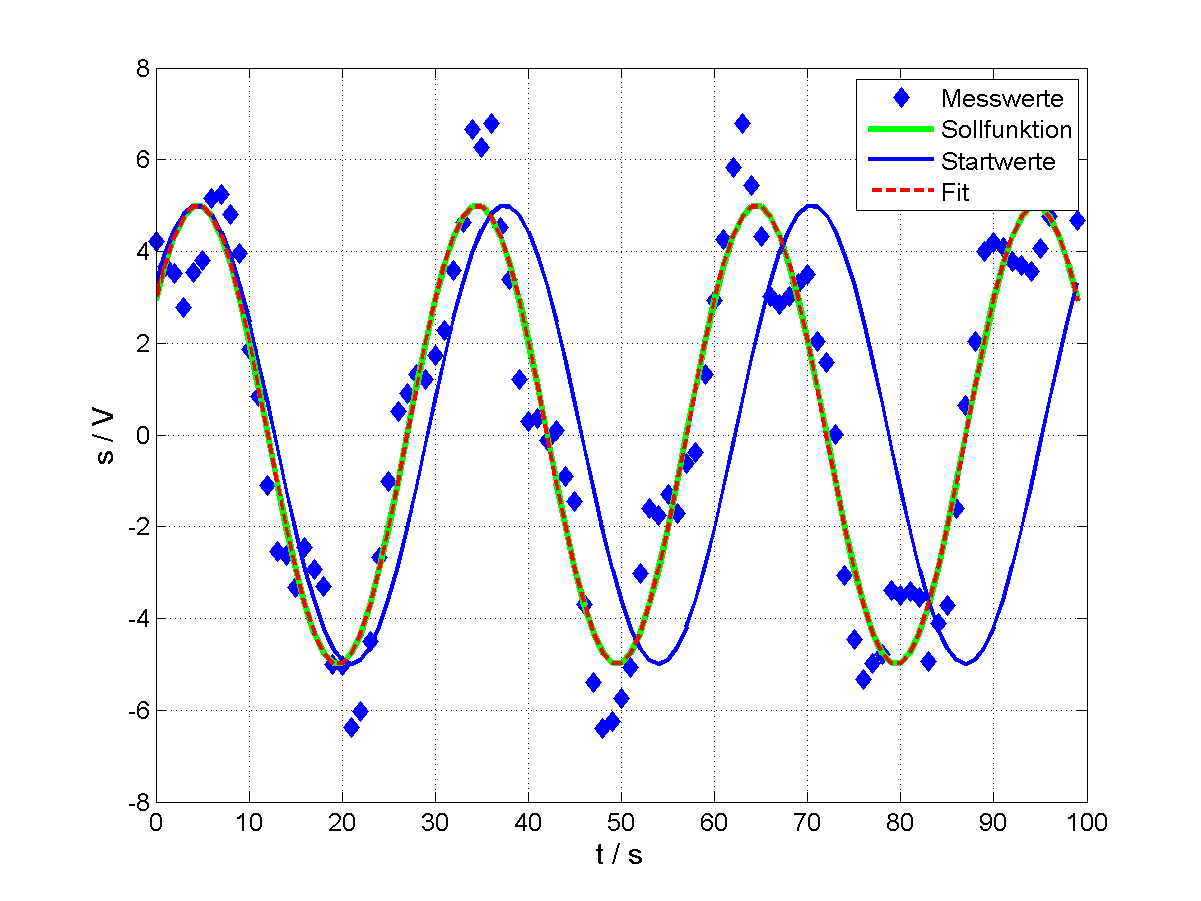
\includegraphics[width=0.8\textwidth, angle = 0]{03_vorlesung/media/pltSS_nonlin_leastsquare_sin_zB2.png}
\end{center}
\caption{Beispiel eines sinusförmigen Signals mit Levenberg-Marquadt-Fit gemäß
Gln.~(\ref{ZielfunktionalGradTaylorResiDaempf}) und (\ref{DaempfTuning}) zusammen mit
den Entscheidungen aus Tabelle 1.\label{LSoptiExampleSinusFitted}}
\end{figure}

Dieses Beispiel hat einen Modellansatz
\begin{equation}
s(t) \; = \; a \sin(2\pi \frac{t}{\lambda} + \varphi) \; + \; \varepsilon \qquad 
\textrm{mit} \qquad \varepsilon \sim {\cal N}(0,\sigma) 
\end{equation}
bei dem die Residuen in Richtung von $s$ streuen und bei dem die Abtastpunkte
entlang der Zeitachse $t$ als Regressor vorgegeben sind, so dass
wir einen Regressionsansatz der Gestalt
\begin{equation}
\epsilon_j \; = \; Y_j \; - \; f(X_j, \boldsymbol{\theta}) \qquad \textrm{mit} \qquad 
j=1, 2,\dots, J 
\end{equation}
vorliegen haben. Die Kostenfunktion sieht damit wie folgt aus
\begin{equation}
Q \; = \; \sum\limits_{j=1}^J \left(Y_j \; - \; f(X_j, \boldsymbol{\theta})\right)^2.
\end{equation}
Für die nichtlineare Regression gibt es in Gnu-Octave  beispielsweise folgende
Funktion:
\begin{verbatim}
[f, p, cvg, iter] =leasqr (x, y, init, F);
\end{verbatim}
Angewendet auf unser Beispiel vom sinusförmigen Signal kann sie in folgender Weise
verwendet werden
\begin{verbatim}
function fit_sin(gen_new)
 % Stand: 191105
 % Läuft nur unter Octave, da leasqr nur unter Octave
 % frei zur Verfügung steht. Bei Matlab gibt es
 % einen ähnlichen Befehl, der heisst nlinfit
  load('pltSS_nonlin_leastsquare_sin_zB2.mat');
  p0 = [34; 0.23*pi];
  sf = @(x, p) a*sin(2*pi*x/p(1) + p(2));
  [f1, p1, kvg1, iter1, corp1, covp1, covr1, stdresid1, Z1, r21] = ...
  leasqr (t(:), s(:), p0, sf);
  fprintf(stdout,'gefittete Werte: lambda = %1.2f;  phi/pi = %1.2f\n', ...
  p1(1), p1(2)/pi );
  t = [0:99]'; % Sekunden
  N = length(t);
  %
  a = 5; % Volt
  lam = 30; % Sekunden
  sigma = 0.13*a;
  phi = 0.2*pi;
 %
  am = 0.3*a;
  phim = 0.7*pi;
  lamm = 0.3*lam;
 %
  st = a*sin(2*pi*t/lam + phi);
  figure(1);
  plot( t, s, 'kd', ...
  t, st, 'g-.;soll;', ...
  t, sf(t,p0), 'b--;Startwerte;', ...
  t, sf(t,p1), 'r-;gefittet;');
  xlabel('t / s','fontsize', 14);
  ylabel('s / V','fontsize', 14);
  set(gca,'fontsize',12);
  grid on;
  end
\end{verbatim}
und wir erhalten folgendes Ergebnis
\begin{verbatim}
gefittete Werte: lambda = 30.0505;  phi/pi = 0.2051
\end{verbatim}

\newpage
\section{Matlabfunktionen zur Berechnung nichtlinearer Fits}
Es gibt eine Vielzahl an Bibliotheksfunktionen, die nichtlineare Optimierungsverfahren implementiert haben. So gibt es z.B. 
z.~B. die Matlab-/Octavefunktion \newline \textsf{X = fminbnd(FUN,x1,x2,OPTIONS)}.
\textsf{fminbnd} versucht das lokale Minmimum einer Funktion \textsf{FUN} mit einer
Variablen im Intervall \textrm{x1 $<$ X $<$ x2} zu finden.  
Als \glq OPTIONS\grq~können u.a. gewählt werden TolX (Toleranz, wann abgebrochen
werden soll) oder MaxIter (Maximale Anzahl an Iterationen, die durchgeführt
werden sollen).
Da bei unserem Beispiel mit dem Sinusfit zwei Parameter zu schätzen sind, 
verwenden wir die Funktion \textsf{fminsearch}. Hier wird nur ein Schätzwert (Startwert) 
\textrm{x0} angegeben. Die zu minimierende Kostenfunktion $Q$ ist gegeben durch: 
\begin{equation}
Q(\boldsymbol{p}) = \sum_j (a \cdot \sin(2\cdot \pi \cdot t(j) /p(1) + p(2))-s(j))^2
\;\rightarrow \;\textrm{Min.}
\end{equation}
Der dazugehörige Matlab-Code lautet: 
\begin{verbatim}
load('pltSS_nonlin_leastsquare_sin_zB2.mat');
a = 5; % Volt
p0 = [34; 0.23*pi];
% Ziel-/ Kostenfunktion:
Q = @(p) sum((a*sin(2*pi*t/p(1) + p(2))-s).^2) ;
tol = 1E-15;
maxit =1000;
p1= fminsearch(Q, p0, optimset('TolX',tol, 'MaxIter', maxit));
disp(['gefittete Werte: lambda =', num2str(p1(1)),';  ', ...
num2str(p1(2)/pi)])
\end{verbatim}
Als Ergebnis erhält man: 
\begin{verbatim}
gefittete Werte: lambda =30.0505; phi/pi=0.2051
\end{verbatim}
\begin{figure}[htb]
	\begin{center}
		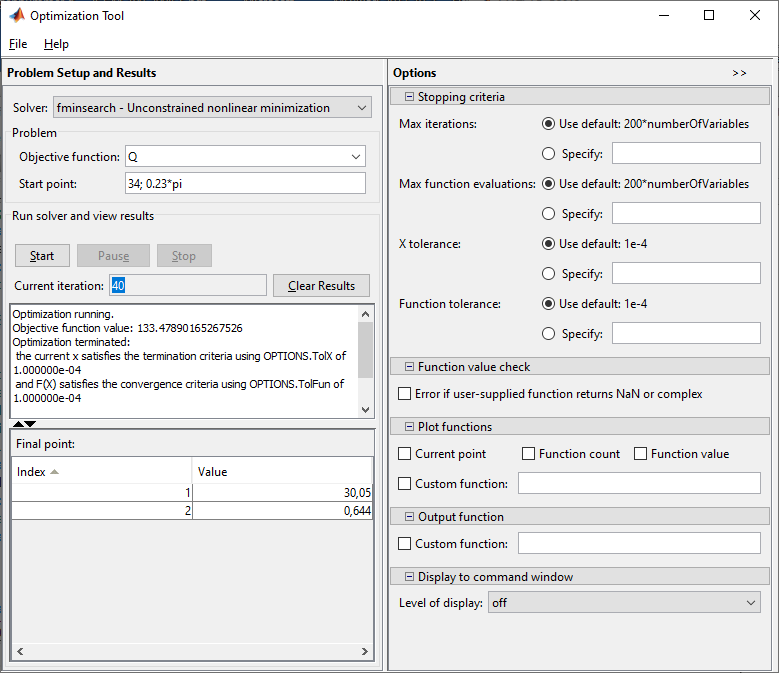
\includegraphics[width=0.9\textwidth, angle = 0]{03_vorlesung/media/OptimToolMatlab.png}
	\end{center}
	\caption{Optimtool von Matlab: Ergebnis $p(1)=30,05$ und $p(2)=0,644$} \label{fig:Optimtool_von_Matlab}
\end{figure}

\newpage
Tabelle \ref*{tab:Optimierungsverfahren} gibt einen Überblick über 
Matlabfunktionen bei Optimierungsproblemen, siehe dazu auch 
S.~S.~Rao \cite{Rao09}. $\mathbf{lb}$ steht für \glq lower bound\grq~ und $\mathbf{ub}$ steht für \glq upper bound\grq~

\begin{table}[!ht]
	\caption{Optimierungsverfahren mit Matlab}
	\centering
	\begin{tabular}{p{5cm} | >{\centering\arraybackslash} p{6cm} | p{4cm}}  \hline 
		Typ des Optimierungs- \newline problem &  Standardform für die Lösung unter Matlab/Octave &  Matlab/Octave Funktion um das Problem zu lösen \\[1ex]
		\hline \hline 
		Funktion von einer  \newline Variablen  & Finde $x$, indem $f(x)$ minimiert wird mit
		$x_1 < x < x_2$ & \textsf{fminbnd} \\[1ex] \hline 
		Minimierung ohne Randbedingung von einer Funktion oder mehreren Variablen &
		Finde $\mathbf x$, so dass $f(\mathbf x)$ minimiert wird.  & 
		\textsf{fminunc} oder \newline \textsf{fminsearch} \\[1ex] \hline 
		Lineares Problem & Finde $\mathbf x $ durch Minimierung von $\mathbf{f^T x}$ mit $A \mathbf x \le b$, $A_{eq} \mathbf x = \mathbf b_{eq}$, \newline
		$\mathbf{lb} \le \mathbf{x} \le \mathbf{ub}$ & \textsf{linprog} \\[1ex] \hline
		Quadratisches Problem & Finde $\mathbf x $ durch Minimierung von $\frac{1}{2} \mathbf{x^T}\mathbf{f^T x}$ mit $A \mathbf x \le \mathbf b$, 
		\newline $A_{eq}$ $\mathbf x = \mathbf b_{eq}$, \newline
		$\mathbf{lb} \le \mathbf{x} \le \mathbf{ub}$ & \textsf{quadprog} \\[1ex] \hline
		Minimierung von Funktionen von mehreren Variablen mit Nebenbedingungen &
		Finde $\mathbf x $ durch Minimierung von $\frac{1}{2} \mathbf{x^T}\mathbf{f^T x}$ mit $\mathbf{c(x) \le 0}$, 
		$\mathbf{c_{eq} = 0}$ \newline
		$A \mathbf x \le \mathbf b$, 
		$A_{eq}$ $\mathbf x = \mathbf b_{eq}$, \newline
		$\mathbf{lb} \le \mathbf x \le \mathbf{ub}$ & \textsf{fmincon} \\[1ex] \hline
		Minimax Problem & Finde das  $\mathbf x $ welches die Maxima
		von mehreren gegeben Funktionen $F_i(\mathbf x)$ minimiert, 
		so dass  $\mathbf{c(x) \le 0}$, 
		$\mathbf{c_{eq} = 0}$ \newline
		$A \mathbf x \le \mathbf b$, 
		$A_{eq}$ $\mathbf x = \mathbf b_{eq}$, \newline
		$\mathbf{lb} \le \mathbf x \le \mathbf{ub}$ & \textsf{fminimax} \\[1ex] \hline
	\end{tabular}
	\label{tab:Optimierungsverfahren}
\end{table}

Bei Matlab gibt es die in Abb. \ref{fig:Optimtool_von_Matlab} gezeigte graphische Oberfläche, das sog.
\glq Optimization tool\grq~(Funktionsaufruf: \glq optimtool\grq),
die die in Tab. \ref*{tab:Optimierungsverfahren} aufgeführten
Optimierungsverfahren und noch einige mehr zur Verfügung stellt.
Dieses Tool eignet sich ganz gut, wenn man sich einen ersten Überblick
über die in Matlab implementierten Optimierungsverfahren verschaffen will. \\

\newpage
\section{Gradientenverfahren mit unterschiedlichen Varianzen}
\label{unterschiedVar}
Die Varianzen (und Kovarianzen) der Residuen sind immer auch Funktion der Modellparameter. Als wir die
Maximum-Likelihood-Methode eingeführt haben, hatten wir sie ausgeklammert und bei der Bestimmung
des Minimums über die Summer der kleinsten Residuenquadrate weggekürzt. Sie
lassen sich für den Fall ausklammern, bei dem die Streuung bezüglich des Modells
für alle Messpunkte gleich ist, also
\begin{equation}
Q(\mathbf{p}) \; = \;
 \frac{\boldsymbol{\varepsilon}(\mathbf{p})^\mathsf{T} \, \boldsymbol{\varepsilon}(\mathbf{p})}{\sigma^2(\mathbf{p}))}
\end{equation}
und
\begin{equation}
\nabla_{\mathbf{p}} Q(\mathbf{p})  \; = \; 
\frac{2}{\sigma^2(\mathbf{p})} \boldsymbol{\varepsilon}^\textsf{T}(\mathbf{p})
 \, \boldsymbol{J} \overset{!}{=} \; \left(\begin{array}{ccc} 0 & \dots & 0 \end{array}\right)
\label{ZielfunktionalGradJmitSigma}
\end{equation}
was einfach mit $\frac{\sigma^2(\mathbf{p})}{2}$ multipliziert werden kann, so dass wir mit
den Residuen wie oben beschreiben weiter arbeiten können, indem wir diese in Taylorreihe entwickeln.

Für den Fall, dass es unterschiedliche Varianzen für Residuen der verschiedenen Beobachtungstupel
$(X_{1,j},\dots,X_{N,j})$ gibt, ordnen wir $\sqrt{\sigma_j^2} = \sigma_j$ 
den Residuen zu mit
\begin{equation}
Q(\mathbf{p}) \; = \;
  \left(\begin{array}{ccc}
  \frac{\varepsilon_1(\mathbf{p})}{\sigma_1(\mathbf{p})} & \dots &
 \frac{\varepsilon_J(\mathbf{p})}{\sigma_J(\mathbf{p})} \end{array} \right)
\, \left(\begin{array}{c} \frac{\varepsilon_1(\mathbf{p})}{\sigma_1(\mathbf{p})}\\
 \vdots\\ \frac{\varepsilon_J(\mathbf{p})}{\sigma_J(\mathbf{p})}\end{array} \right)
\label{ZielfunktionalJmitW}
\end{equation}
d.h.\ kurz ohne jedesmal das \glqq Funktion von $\mathbf{p}$\grqq oder
\glqq abhängig von $\mathbf{p}$\grqq, also $(\mathbf{p})$,
mitzuschreiben
\begin{equation}
Q(\mathbf{p}) \; = \;
  \boldsymbol{\varepsilon}^\textsf{T}
\, \left(\begin{array}{cccc} \frac{1}{\sigma_1^2} & \dots & & 0 \\
  & \ddots & \\
 0 & & \dots &  \frac{1}{\sigma_J^2} \end{array} \right) \, \boldsymbol{\varepsilon}
\label{ZielfunktionalJmitW1}
\end{equation}
Je stärker eine Beobachtung $j$ abweicht, also je größer die Varianz $\sigma_j^2$,
desto geringer fällt der Summand $\frac{\varepsilon_j^2}{\sigma_j^2}$ in der Kostenfunktion $Q$
ins Gewicht, weshalb man diese auch als Gewichte $w_j = \frac{1}{\sigma_j^2}$ bezeichnet
und die Matrix als Gewichtsmatrix $\mathbf{W}$ also
\begin{equation}
Q(\mathbf{p}) \; = \;
  \boldsymbol{\varepsilon}^\textsf{T}
\, \mathbf{W} \, \boldsymbol{\varepsilon}
\label{ZielfunktionalJmitW2}
\end{equation}
und mit
\begin{equation}
\frac{1}{2} \nabla_{\mathbf{p}} Q(\mathbf{p})  \; = \; \boldsymbol{\varepsilon}^\textsf{T}(\mathbf{p})
 \, \mathbf{W} \, \boldsymbol{J}
\label{ZielfunktionalGradJW}
\end{equation}
sieht unser Optimierungsproblem wie folgt aus
\begin{equation}
\lim_{\mathbf{p} \rightarrow \mathbf{\hat p}}
\boldsymbol{\varepsilon}^\textsf{T}(\mathbf{p})
 \, \mathbf{W}(\mathbf{p}) \, \boldsymbol{J}(\mathbf{p})
 \; = \; \left(\begin{array}{ccc} 0 & \dots & 0 \end{array}\right) .
\label{ZielfunktionalGrad1W}
\end{equation}
Die Gleichungen (\ref{GradientQlinGl3}) und (\ref{ZielfunktionalGradTaylorResiDaempf})
werden damit zu
\begin{equation}
 \boldsymbol{J}^{(\kappa) \textsf{T}} \, \mathbf{W}(\mathbf{p}_\kappa) \, 
\boldsymbol{J}^{(\kappa)} \, \Delta \mathbf{p}_\kappa
\; \overset{!}{=} \; 
-  \boldsymbol{J}^{(\kappa) \textsf{T}} \, \mathbf{W}(\mathbf{p}_\kappa) \, 
\boldsymbol{\varepsilon}(\mathbf{p}_\kappa) .
\label{GradientQlinGl3W}
\end{equation}
und mit Dämpfungs- bzw.\ Marquardtparameter
\begin{equation}
\left(
\boldsymbol{J}^{(\kappa) \textsf{T}} \, \mathbf{W}(\mathbf{p}_\kappa) \, \boldsymbol{J}^{(\kappa)}
 + \mu \, \mathrm{diag}(\boldsymbol{J}^{(\kappa) \textsf{T}} \, \mathbf{W}(\mathbf{p}_\kappa) \, \boldsymbol{J}^{(\kappa)}) \right) \Delta \mathbf{p}_\kappa \;
\overset{!}{=} \; - \boldsymbol{J}^{(\kappa)^\textsf{T}} \, 
\mathbf{W}(\mathbf{p}_\kappa) \, \boldsymbol{\varepsilon}(\mathbf{p}_\kappa) .
\label{ZielfunktionalGradTaylorResiDaempfW}
\end{equation}

Es gibt aber auch Fragestellungen mit unterschiedlichen Varianzen $\sigma_i^2$ 
zu den direkten Messgrößen $X_i$. Ein Beispiel dafür
\begin{figure}
\begin{center}
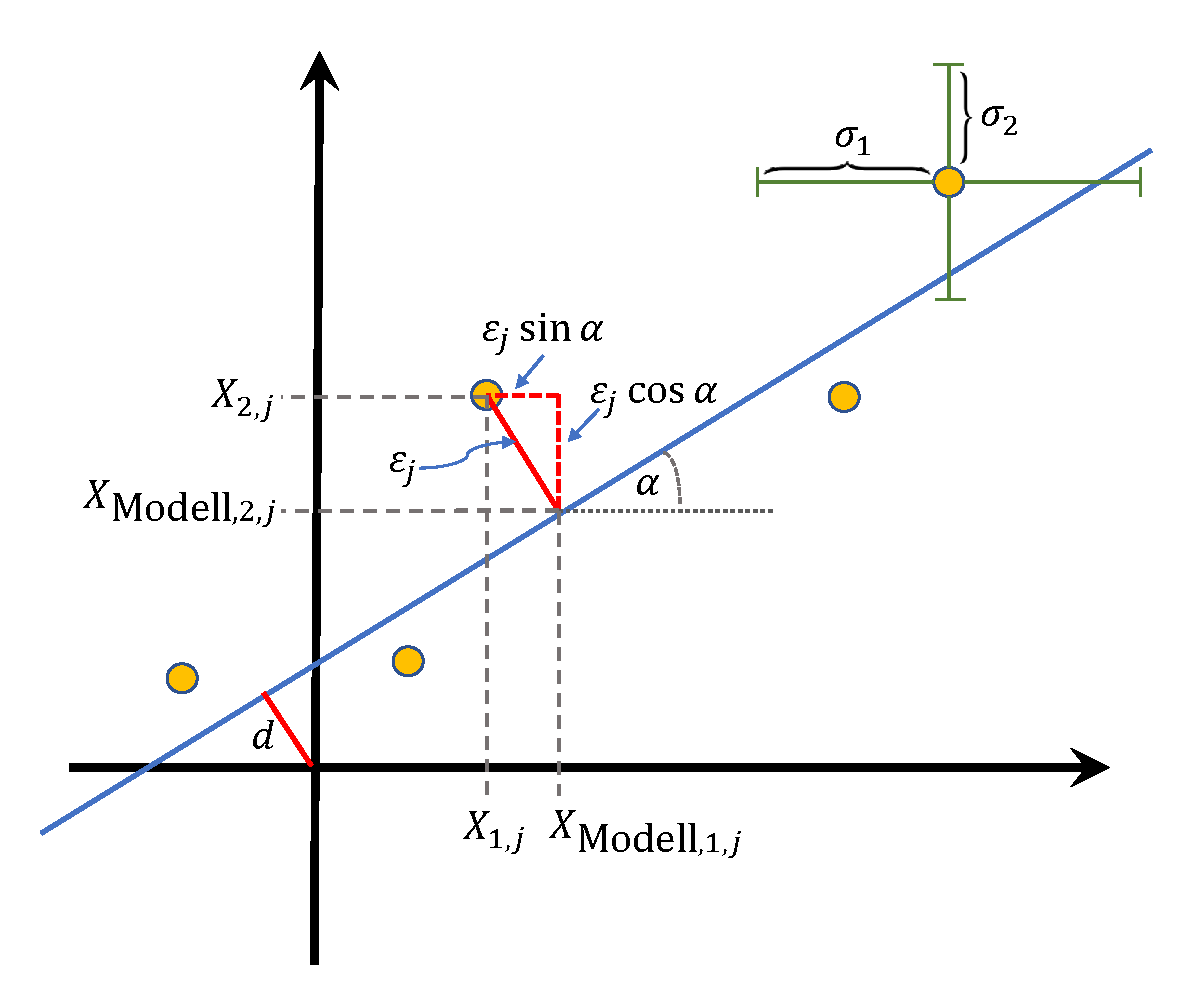
\includegraphics[width=100mm]{03_vorlesung/media/ResiduenVarianzen.pdf}
\end{center}
\caption{Veranschaulichung für Schätzung von Geradenparametern durch
Minimierung der Summe der Quadrate der Residuen bei verschiedenen Varianzen 
$\sigma_1^2$ und $\sigma_2^2$ der beiden direkten Messgrößen $X_1$ und $X_2$
\label{ResiduenVarianzen}}
\end{figure}
ist eine Gerade in einer Ebene mit den Modellparametern $\alpha$ für den Winkel und
$d$ für den Abstand der Geraden vom Koordinatenursprung
\begin{equation}
\varepsilon_j \; = \; 
\left(\begin{array}{c} X_{1,j}\\ X_{2,j}\end{array}\right) \cdot
\left(\begin{array}{c} -\sin(\alpha)\\ \cos(\alpha)\end{array}\right) \; - \; d .
\label{TLSgerade}
\end{equation}
Hier stehen die Residuen $\varepsilon_j$ des $j$-ten Messpunktes $(X_{1,j}, X_{2,j})$ 
senkrecht auf der Modellgeraden, siehe Abb.~\ref{ResiduenVarianzen}, weil beide
Messgrößen $X_1$ und $X_2$ gleichermaßen Zufallsgrößen sind und nicht eine davon
ein Regressor ist die andere ein Regressand ist. Bei dieser \textsl{Least-Square} Methode
spricht man auch von \textsl{Total Least-Square} Methode, weil \glqq total\grqq ~alle Größen
streuen können, also Zufallsgrößen sind.

\begin{equation}
Q(\alpha, d) \; = \;
\sum\limits_{j=1}^J \,  \left(\frac{\varepsilon_j(\alpha, d) \sin(\alpha)}{\sigma_1}\right)^2
\; + \; \sum\limits_{j=1}^J \, \left(\frac{\varepsilon_j(\alpha, d) \cos(\alpha)}{\sigma_2}\right)^2 .
\end{equation}
Hier haben wir also die $\sigma_i^2$ als Varianzen der Abweichungskomponenten
der Messgröße $X_i$ (vektorwertige Residuen!) für alle $j=1,\dots,J$ Beobachtungen
und nicht Varianzen $\sigma_j^2$ für das skalarwertige Residuum der $j$-ten Beobachtung.
Die allgemeine Form mit Kovarianzen sieht dann also so aus
\begin{equation}
Q(\mathbf{p}) \; = \;
 \sum\limits_{j=1}^J \, \vec \varepsilon(X_{1,j},\dots,X_{N,j},\mathbf{p})^\mathsf{T} \, 
\boldsymbol{\Sigma}(X_{1,j},\dots,X_{N,j},\mathbf{p})^{-1} \, \vec \varepsilon(X_{1,j},\dots,X_{N,j},\mathbf{p})_j .
\label{generalLSmethod}
\end{equation}
In diesem Zusammenhang erfolgt die nichtlineare Optimierung, indem nicht
die Residuen in Taylorreihe entwickelt, sondern die Gradientenfunktion $\nabla Q$ direkt.

\section{Robuste Schätzverfahren}
\label{robustEstimation}
Wir haben nun eine Kostenfunktion $Q$ mit Gewichtsfaktoren kennengelernt, Gl.~(\ref{ZielfunktionalJmitW2}),
bei der die Gewichte die Kehrwerte der Varianzen sind $w_j = \frac{1}{\sigma_j^2}$, die sich eigentlich
aus der Abweichung der Beobachtungen vom Modell ergeben. Wenn kein {\`a} priori Wissen über
diese Varianzen vorliegt, aber bekannt ist, dass die Verteilung der
Residuen aller Beobachtungen nicht gauß\-ver\-teilt ist, soll das Problem dennoch mit der
Maximum-Likelihood-Methode gelöst werden. Es kommt vor, dass einzelne Beobachtungen
sehr weit von der Erwartung entfernt sind. Man sagt, dass sie signifikant abweichen. Die Gaußverteilung erlaubt dieses auch, denn sie hat einen Definitionsbereich für die Residuen $\varepsilon$,
der von minus Unendlich bis plus Unendlich geht, ihre Ausläufer auch \textsl{Tails} genannt,
sind unbegrenzt. Die Wahrscheinlichkeit ist aber sehr gering, kleiner als $5~\%$, dass der Betrag der
Residuen $\varepsilon$ einen Wert annimmt, der größer als
$1.65 \, \sigma$ ist, aber er kann auftreten. Liegen deutlich mehr als $5~\%$
der Beobachtungen außerhalb eines Vertrauensintervalls von beispielsweise $[-3 \sigma, 3 \sigma]$,
dann ist dies ein Indiz dafür sein, dass das Modell unzureichend ist. Es kann sein, dass es auch nicht
um ein vollständigeres Modell geht, sondern darum, nur die zum betrachteten Modell passenden Beobachtungen
berücksichtigen zu wollen. Die übrigen Beobachtungen sollen als Ausreißer, die nicht zum
eigentlichen zu untersuchenden Prozess gehören, nicht an dem \textsl{Least-Square-Fit}
beteiligt werden oder zumindest ihre Beteiligung daran (ihr Gewicht) reduziert wird.

Die Idee für die Realisierung dieser Aufgabe ist, die Verteilung der Residuen durch Umgewichten so zu verändern, das
sie wieder die Gestalt einer Normalverteilung bekommt. Wir führen Gewichtsfaktoren $w = \delta$ ein,
die eine Funktion des Abstands $\varepsilon$ einer Beobachtung vom Modell ist, so dass die Wahrscheinlichkeitsdichte 
der Abweichung $\tilde \varepsilon$ einer Normalverteilung folgt. Gesucht ist eine Gewichtsfunktion
$\delta \! : \varepsilon \mapsto \delta(\varepsilon)$ für die gilt
\begin{equation}
\tilde \varepsilon \; = \; \delta(\varepsilon) \; \varepsilon \quad \Rightarrow
\quad \tilde \varepsilon \sim {\cal N}(0,\sigma) .
\end{equation}
Mit Hilfe der Gewichtsfunktion werden aus den Residuen die Gewichtsfaktoren
$w_j = \delta_j = \delta(\varepsilon_j)$ berechnet. Da man die Residuen erst nach
Schätzung der Modellparameter gewinnt, erfordert dies wie bei der nichtlinearen Optimierung
auch sonst, einen iterativen Prozess.

Wir betrachten folgende Kostenfunktion
\begin{equation}
Q(\mathbf{p}) \; = \; \sum_{j=1}^J \, \delta_j \, \varepsilon_j(\mathbf{p})^2 .
\label{robustEstim}
\end{equation}

Zunächst werden die Parameter ungeachtet möglicher Ausreißer mittels \textsl{Least Square}-Methode
ohne Gewichte
\begin{equation}
 \min_{\mathbf{p}} Q(\mathbf{p}) \qquad \mathrm{mit} \qquad 
Q(\mathbf{p}) \; = \; \sum_{j=1}^J \, \varepsilon_j(\mathbf{p})^2 .
\label{linEstim}
\end{equation}
geschätzt mit $\mathbf{p}_0$.

Wir betrachten wieder ein einfaches Beispiel, in dem es nur einen Parameter $y$ gibt und eine 
Messgröße $X_1$ mit $J$ Beobachtungen $(X_{1,1},\dots,X_{1,J})$.
Dabei wird davon ausgegangen, dass die Beobachtungen zu einer Grundgesamtheit, also zu einem Parameter gehören.
Die Beobachtungswerte werden histogrammiert. Das Histogramm ist in Abb.~\ref{biasExampleKap3} dargestellt.
\begin{figure}
\begin{center}
\includegraphics[width=90mm]{03_vorlesung/media/learn_robust.pdf}
\caption{Beispiel für nicht erwartungsgemäße Beobachtungen}
\label{biasExampleKap3}
\end{center}
\end{figure}
Für das Histogramm werden $K \, = \, 80$ Klassen (engl.\ \textsl{bins}) gewählt, die Anzahl der Beobachtungen umfasst $J \, = \, 2200$.
Die Klassenbreite ist dann
\begin{equation}
\Delta \xi \; = \; \frac{1}{K} \left( \max \left\{X_{1,j}\right\} \; - \; \min \left\{X_{1,j}\right\} \right)
\end{equation}
so dass $K+1$ Klassengrenzen $\xi_{\mathrm{G}, k}$ vorliegen,
deren Indizes wir von Null bis $K$ zählen:
\begin{equation}
 \xi_{\mathrm{G}, k} \; = \; k \, \Delta \xi \; + \; \min \left\{X_{1,j}\right\}
\qquad k = 0, \dots, K
\label{limkthbin}
\end{equation}
und die Mitte in der jeweiligen Klasse für den Wert der Klasse verwenden
\begin{equation}
 \xi_k \; = \; k \, \Delta \xi  \, + \, \frac{1}{2} \Delta \xi  \; + \; \min \left\{X_{1,j}\right\}
\qquad k = 1, \dots, K
\label{kthbin}
\end{equation}
wobei die Anzahl der Klassen $K$ ist.

Die Anzahl der Einzelbeobachtungen, für die gilt
\begin{equation}
\xi_{\mathrm{G}, k-1} \; \leq \; X_{1,j} \; <  \xi_{\mathrm{G}, k},
\end{equation}
nennen wir \textsl{Häufigkeit} $n_k$. Bei der letzten Klasse, also für
$k = K$ wird auch bei der rechten Intervallgrenze ein $\leq$.
Damit ist die diskrete Funktion $n(\xi)$ die Häufigkeitsverteilung.

Der Schätzwert für den Parameter ist nach der Maximum-Likelihood / Least-Square-Methode der
Mittelwert, der hier den Wert $25.47$ annimmt. In Wirklichkeit gehören die Beobachtungswerte gar nicht zu
nur einer Grundgesamtheit, sondern $1750$ gehören zu dem Parameter $\mu_1 \, = \, 23.00$ und $450$ zu $\mu_2 \, = \, 35.00$.
Diese Wirklichkeit kennt aber niemand. Bei Betrachten des Histogramms sieht der Messtechniker jedoch, dass ein
Nebenmaximum vorliegt, es keine reine Gaußverteilung ist. Die weiter entfernt liegenden Beobachtungen sollen unterdrückt werden
durch entsprechende Wahl zugehöriger Gewichtsfaktoren $\delta_j$.

Eine mögliche Wahl für die Gewichtsfaktoren ist die \textsl{Tuckey biweight}-Funktion.
\begin{equation}
\delta_j \; = \;
\left\{ \begin{array}{cl}
\left( 1 \, - \, \left( \frac{X_{1,j} \, - \, y^{(\kappa)}}{c^{(\kappa)}} \right)^2 \right)^2 & 
	\mathrm{falls} \; \mid X_{1,j} \, - \, y^{(\kappa)} \mid \, \leq \, c^{(\kappa)} \\
0 & \mathrm{sonst}
\end{array} \right.
\end{equation}
wobei $\kappa$ der Zähler für den Iterationsschritt ist und $c^{(\kappa)}$ ein passend zur Anwendung zu wählender Faktor ist, hier beispielsweise
\begin{equation}
c^{(\kappa)} \; = \; \mathrm{median} \mid X_{1,j} \, - \, y^{(\kappa)} \mid 
\end{equation}
Die Kostenfunktion, deren Gewichte von den iterativ bestimmten Residuen und damit von den
iterativ geschätzten Parametern abhängt, stellt ein nichtlineares Optimierungsproblem
$ \min_{\mathbf{p}} Q(\mathbf{p}) $ dar, mit
\begin{equation}
Q(\mathbf{p}) \; = \; \sum_{j=1}^J \; \varepsilon_j^2 \;
\left( 1 \, - \, \left( \frac{\varepsilon_j(\mathbf{p}) }{c(\mathbf{p})} \right)^2 \right)^2 \;
H(\mid \varepsilon_j(\mathbf{p}) \mid - c(\mathbf{p})) \;
H(c(\mathbf{p}) - \mid \varepsilon_j(\mathbf{p}) \mid ),
\label{robustEstim2}
\end{equation}
wobei $H$ für \textsl{Heaviside}- oder Sprungfunktion steht.

\begin{figure}
\begin{center}
\includegraphics[width=100mm]{03_vorlesung/media/learn_robust_2.pdf}
\caption{\label{RobustIter} Umgewichten um die Verteilungform der Normalverteilung anzupassen}
\end{center}
\end{figure}

Der Median von den Absolutbeträgen der Residuen $\varepsilon_j \, = \, X_{1,j} \, - \, y^{(\kappa)}$ wird dadurch gewonnen,
dass man die Werte der Größe nach sortiert und dann den mittleren nimmt, also den, auf dem Platz in der Mitte der sortierten
Anordnung liegt.
Abb.~\ref{RobustIter} stellt die ursprüngliche Häufigkeitsverteilung aus Abb.~\ref{biasExampleKap3} als
durchgezogene, schwarze Linie dar. Nach dem ersten Iterationsschritt der Umgewichtung, hat sich die Verteilung so verändert,
wie es durch die blaue gestrichpunktete Linie gezeigt wird, zu der ein Mittelwert von $24.20$ gehört. Nach mehr als acht Iterationen
wurde ein Mittelwert von $23.23$ erzielt und die mit rot gestrichelter Verteilungskurve eingezeichnet sind.

%
\chapter{Konzepte der Statistik für die Messdatenanalyse}
\label{KonzepteinverseProbleme}

\section{Konzepte zum Lösen inverser Probleme}

In den letzen drei Kapiteln (Vorlesungswochen) haben wir einen Einblick in die
Vorgehensweise der Maximum-Likelihood-Methode erhalten:
\begin{enumerate}
\item Die Idee von \textsl{Modell} und \textsl{Lösen inverser Probleme} wurde
  genannt.
\item Zur Lösung inverser Probleme wurde das Schätzen von Parametern, die
 linear in die Modellgleichung eingehen, durch \textsl{lineare Regression} vorgestellt.
\item Ein Einblick in mögliche Verfahren zur Lösung inverser Probleme durch
  Schätzen von Parametern, die nicht-linear in die Modellgleichung eingehen,
  wurde gegeben. Hier wurden kurz drei Verfahren zur \textsl{nicht-linearen Optimierung}
  vorgestellt.
\end{enumerate}
Wir haben dabei gesehen, dass es bei der Messdatenanalyse um die Schätzung von
physikalischen Größen geht, die indirekt über das Messen anderer Größen,
direkter Messgrößen, ermittelt werden.
Die Aufgabe der Messtechnik lässt sich auch beschreiben als die Bestimmung
des Wertes von physikalischen Größen durch Messverfahren, die auf
physikalischen Prinzipien basieren. Die von einem Sensorsystem angezeigten
Größen sind dabei im allgemeinem andere Größen als diejenigen, die zu messen sind.

Wir hatten in der ersten Vorlesung, in Abschnitt \ref{ModelleStatistik},
das Beispiel \glqq Beugung am Gitter\grqq ~betrachtet, 
um die Aufgabenstellung zu verstehen, dass man
aus den einem Messsystem direkt zugänglichen Größen die gesuchten physikalischen
Größen gewinnen möchte. Dabei wurde der Begriff des \textsl{Lösens inverser Probleme}
eingeführt. Nachdem wir bereits Methoden zur Ermittlung von indirekten
Messgrößen als Modellparameter kennen gelernt haben, haben wir die Chance uns
unter den Ideen dieses Konzeptes mehr vorstellen zu können.

Darüber hinaus wurde in Abschnitt \ref{ModelleStatistik} schon mal erwähnt, dass
es etwas unterschiedliche Konzepte oder Heransgehensweisen für Schätzverfahren gibt.
Auf der einen Seite steht der sogenannte \textsl{frequentistische} Ansatz, bei dem allein
Beobachtungswerte direkter Größen verwendet werden und die Annahmen über die
Verteilung der Streuung der direkten Größen impliziet schon ins Schätzverfahren
selber eingebaut ist. Der Begriff Frequenz von englischen \textsl{frequency} übernommen
heißt hier \textsl{Häufigkeit} und nicht \textsl{Frequenz} wie wir das im Deutschen
vielfach mit einer periodischen Bewegung verbunden verstehen. Aber auch die
Deutsche Sprache kennt die Sprechweise: \glqq Dies oder jenes Restaurant oder so
wird gut frequentiert\grqq ~im Sinne von \glqq wird häufig besucht\grqq.

Eine Verallgemeinerung der Schätzmethoden wurde in den letzten Jahrzehnten
in die Messdatenanalyse eingeführt, bei der auch die Modellparameter selber als
Zufallsgrößen behandelt werden. Auch ihnen wird eine Streuung, also
Wahrscheinlichkeitsverteilung zugrunde gelegt. Bei diesen Verfahren lassen sich
Schätzwerte und Werte zur Unsicherheit der Modellparameter in die aktuelle
Schätzung mit einbeziehen. Diese verallgemeinerten Methoden, die die Modellparameter
als Zufallsgrößen betrachten, werden \textsl{bayesische} Methoden genannt.

Bevor wir diese beiden Ansätze (frequentistisch und bayesisch) gegenüber
stellen und vergleichen, wollen wir folgende
zwei Blickrichtungen, messtechnische Aufgaben zu betrachten, beleuchten:
\begin{itemize}
\item als Modell von der Physik des Messprinzips gemeinsam mit dem statistischen
Modell, dass die Größen Zufallsgrößen sind,
\item als inverses Problem.
\end{itemize}
Ein Modell wird dargestellt durch eine Vorstellung darüber, wie die
indirekten Messgrößen $Y_m$ mit den direkten Messgrößen $X_i$ verknüpft sind:
\begin{equation}
(Y_1, \dots, Y_M) \xrightarrow{\mathrm{Modell}} (X_1, \dots, X_N)
\label{forwardModel}
\end{equation} 
\begin{figure}
\begin{center}
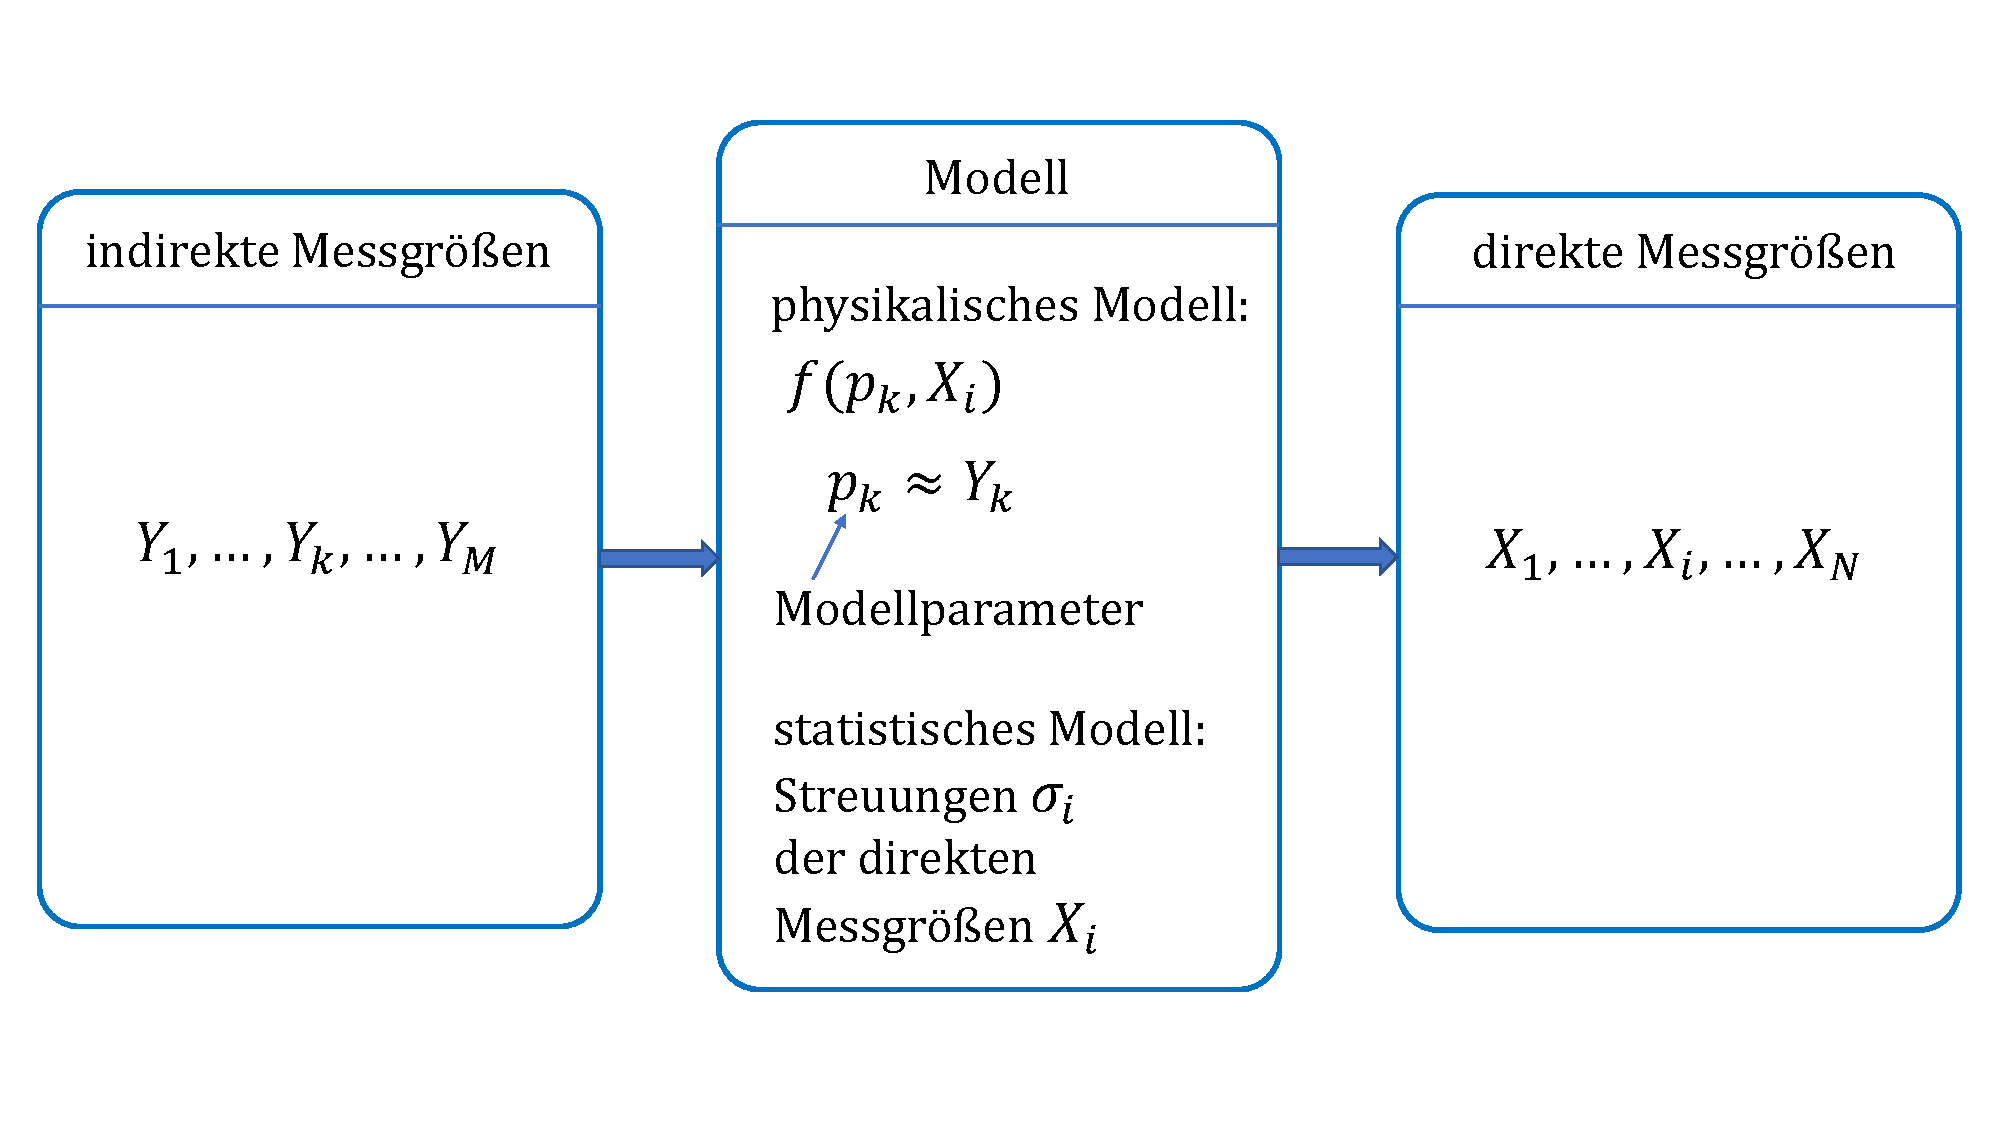
\includegraphics[width=0.8\textwidth, angle = 0]{04_vorlesung/media/Modell1.pdf}
\end{center}
\caption{Modellbildung zur Gewinnung indirekter Messgrößen aus direkten Messgrößen}
\end{figure}

Ein Messvorgang liefert Beobachtungen zu den direkten Messgrößen.
Die wahren Werte der indirekten Größen bleiben verborgen. Die
indirekten Größen können nur geschätzt werden, oftmals auch nur approximiert werden,
weil die Modelle den physikalischen Sachverhalt nur annähernd beschreiben;
denn die Realität ist deutlich komplexer und wird von vielfältigen Einflussfaktoren
bestimmt. Die approximierenden und zufällig streuenden Größen, die die indirekten Messgrößen
repräsentieren, sind die Modellparameter.
Die Abweichungen der Modellparameter entstehen also zum einen
durch vereinfachende Modellannahmen und zum anderen durch zufällige Einflüsse wie das
thermische Rauschen von Elektronik oder Vibrationen im Laborraum.

Im vorigen Kapitel hatten wir bereits den Bezeichner $\mathbf{p}$ für die Modellparameter
verwendet: $\mathbf{p} = (P_1, \dots, P_M)$.
Der Buchstabe $\mathbf{p}$ steht hier einfach nur für den Anfangbuchstaben
von dem Begriff Parameter und der Fettdruck weist darauf hin, dass es ein Vektor mit vielen
Einzelparametern sein kann und dient ferner dazu, das Symbol von dem für die Wahrscheinlichkeitsdichte
zu unterscheiden. Diese wird mit $p$ für den Anfangsbuchstaben von \textsl{probability} bezeichnet.
Für die einzelnen Parameter $P_m$ verwenden wir hier den Großbuchstaben, um die Unterscheidung zur
Wahrscheinlichkeitsdichtefunktion zu haben, sowie in Anlehnung an die Konvention Großbuchstaben
$X_i$ und $Y_m$ für die Messgrößen zu verwenden.
\begin{equation}
P_1 \approx Y_1, \dots, P_M \approx Y_M
\end{equation}
Der Schätzvorgang wird als \textsl{Lösen eines inversen Problems} interpretiert.
\begin{equation}
(X_1, \dots, X_N) \xrightarrow{\mathrm{inverses \; Problem}} (Y_1, \dots, Y_M)
\label{inverseProblem}
\end{equation}

Dazu haben wir die \textsl{Maximum-Likelihood}-Methode kennen gelernt, und gesehen, wie
aus ihr die Methode der kleinsten Residuenquadratsumme hervorgeht. Die Wahrscheinlichkeit,
dass ein Messwert um den Wert $\varepsilon$ von dem geschätzten Modell abweicht, folgt
einer Normalverteilung. Mit anderen Worten kann man auch sagen, dass
die Verteilung der Residuen eine Gaußverteilung ist.
Die Begriffe Gaußverteilung und Normalverteilung verwenden wir synonym.
\begin{equation}
p(\varepsilon | \theta_1,\dots,\theta_M, \sigma) \; = \; \frac{1}{\sigma \sqrt{2 \pi}}
e^{-\frac{1}{2} \left(\frac{\varepsilon}{\sigma}\right)^2}
\label{Maximumlikelihood1}
\end{equation}
Die Symbolik $p(\varepsilon | \theta_1,\dots,\theta_M, \sigma)$ wird gesprochen:
\begin{quote}
Wahrscheinlichkeit $p$ des Eintretens des Ereignises $\varepsilon$
gegeben die Parameter $\theta_1,\dots,\theta_M$ und $\sigma$.
\end{quote}
Der Sprachgebrauch \glqq Eintretens des Ereignisses $\varepsilon$\grqq ~stellt die
Sprechweise der Statistik dar. In den angewandten Wissenschaften, Messtechnik,
Elektrotechnik, etc.\ spricht man von der Wahrscheinlichkeit, dass die Messgröße
oder hier die Abweichung der Messgröße vom Modell einen Wert $\varepsilon$ annimmt oder
dass dieser Wert \glqq beobachtet\grqq ~wird.

In Kapitel \ref{KapitellinReg} wurden Sie mit der Regressionsrechnung vertraut gemacht, die
eine spezielle Anwendung der Maximum-Likelihood-Methode darstellt, bei der
Größen beteiligt sind, die keine Zufallsgrößen darstellen, die Regressoren.
Die Residuen und entsprechend die Regressanden sind die Zufallsgrößen,
für die die in Gl.~(\ref{Maximumlikelihood1}) formulierte Wahrscheinlichkeitsdichte
angenommen wird.
Diese Modellannahme, dass die \textsl{Residuen} als normalverteilt seien,
hatten wir in Abschnitt \ref{RegressionsIdee} wie folgt formuliert:
\begin{quote}
Die abhängigen Größen $Y$, d.h.\ die \textsl{Regressanden} streuen und ihre Residuen sind
	normalverteilt mit Erwartungswert $E(\varepsilon) = 0$ und Varianz $\mathrm{Var}(\varepsilon) = \sigma^2$. 
	Die Residuen sind \textsl{unabhängig und identisch verteilt}, kurz u.i.v.
	\begin{equation}
	\varepsilon \; \overset{\mathrm{u.i.v.}}{\sim} \; \mathcal{N}(0,\sigma) .
	\label{Resinormalverteilt}
	\end{equation}
\end{quote}
Ein Residuum der linearen Regression mit $Y$ als Regressand und $X_i$ als Regressoren
hat folgende Gestalt
\begin{equation}
\varepsilon_j \; = \; Y_j \; - \; \sum\limits_{i=1}^{M} \theta_i \, X_{i,j}
\end{equation}
wobei der Bezeichner $Y$ der Regressionsrechnung die direkte Messgröße ist und die
Regressoren ebenfalls zu den direkten Größen gehören, jedoch nicht als Zufallsgrößen mit
Streuung, sondern mit vorgegebenen, deterministischen Werten.

Ein Residuum nach der Methode der kleinsten Quadrate für ein Modell mit genau nur einer
einzigen Zufallsgröße $X$ mit einem Modellparameter $\mu$ ist einfach
\begin{equation}
\varepsilon_j \; = \; X_j \, - \, \mu .
\label{oneQuantityOnly1}
\end{equation}

Ein Residuum nach der Methode der kleinsten Quadrate für ein Modell ohne Regressoren,
also mit allen beteiligten Größen als Zufallsgrößen, lässt sich allgemein nicht mit
einem Ansatz darstellen, in dem die Modellparameter linear sind. In Abschnitt
\ref{unterschiedVar} haben wir gesehen, dass bereits bei einer
Geraden, für die sowohl die Abzissengröße $X_1$ als auch die Ordinatengröße $X_2$ streut,
die Modellparameter nichtlinear in die Kostenfuntion eingehen.
Die Modellparameter sind der Steigungswinkel $\alpha$ der Geraden relativ zur Abzisse und
der Abstand $d$ der Geraden vom Koordinatenursprung. Das Residuum $\varepsilon_j$ stellt den
Abstand des $j$-ten Messpunktes $(X_{1,j}, X_{2,j})$ zum Modell dar, siehe Abb.~\ref{ResiduenVarianzen}.
\begin{equation}
\varepsilon_j \; = \; 
\left(\begin{array}{c} X_{1,j}\\ X_{2,j}\end{array}\right) \cdot
\left(\begin{array}{c} -\sin(\alpha)\\ \cos(\alpha)\end{array}\right) \; - \; d .
\label{TLSgerade4}
\end{equation}
Wir haben in vorherigen Kapitel gesehen, dass 
bei der Lösung von inversen Problemen, bei denen im Gegensatz zur linearen
Regression eine nichtlineare Verknüpfung der Modellparameter vorliegt,
die Parameter nicht mehr durch Lösen eines linearen Gleichungssystems
bestimmen werden können.
Die Schätzung von Modellparametern besteht dann darin, die Modellparameter auszuprobieren,
d.h.\ viele unterschiedliche Werte vorzugeben,
\begin{equation}
(P_1, \dots, P_M) \xrightarrow{\mathrm{Modell}} (X_{\mathrm{Modell},1,j}, \dots, X_{\mathrm{Modell},N,j})
\label{forwardModel2}
\end{equation} 
 und das Ergebnis der 
Modellrechnungen (\ref{forwardModel2}) mit den beobachteten Werten zu vergleichen, solange,
bis das Ergebnis \glqq gut zu den beobachteten Werten passt\grqq, die Kostenfunktion minimal wird.
Wir haben dazu im vorigen Kapitel einen Einblick erhalten, wie numerische entsprechende 
Optimierungsverfahren prinzipiell funktionieren.
Im Fall der linearen Regression repäsentiert $\mathbf{p} = (\theta_1,\dots,\theta_M)$,
im Fall der Geraden $\mathbf{p} = (\alpha, d)$ und im Fall der Einzelgröße
$\mathbf{p} = \mu$.

Die beiden Annahmen, dass - wie wir in Kapitel \ref{KapitellinReg} bereits bei der linearen Regression
aufgeschrieben hatten - jede einzelne Beobachtung unabhängig und identisch verteilt 
(u.i.v) ist, sind Voraussetzung der Maximum-Likelihood-Methode:
\begin{itemize}
\item Jeder Messpunkt wurde unabhängig von allen anderen gewonnen.
\item Jeder Messpunkt ist identisch verteilt (sie haben die gleiche Streuung).
\end{itemize}

Die gemeinsame Wahrscheinlichkeitsdichte, engl.\ \textsl{joint probability density}, der
Residuen von $j$ voneinander unabhängigen Messungen ist dann das Produkt der
Wahrscheinlichkeitsdichten $p(\varepsilon_j | \mathbf{p}, \sigma)$
jedes Residuums:
\begin{equation}
p(\varepsilon_1,\dots,\varepsilon_J | \mathbf{p}, \sigma) \; = \; 
\prod\limits_{j = 1}^J \, p(\varepsilon_j | \mathbf{p}, \sigma) \; = \; 
 \frac{1}{(\sigma \sqrt{2 \pi})^J} \prod\limits_{j = 1}^J \, 
e^{-\frac{1}{2} \left(\frac{\varepsilon_j}{\sigma}\right)^2}.
\end{equation}
Anhand des kleinen Beispiels mit dem ohm'schen Gesetz haben wir in Abschnitt \ref{ModelleStatistik}
gesehen (Gln.~(\ref{MaxiLikeR1}), (\ref{MaxiLikeR2}) und Gl.~(\ref{MaxiLikeLSQ})),
wie die Maximum-Likelihood-Methode in die Methode der kleinsten Summe der
Residuenquadrate überführt wird:
Unter Anwendung des Potenzgesetzes wird das Produkt der Wahrscheinlichkeiten also
\begin{equation}
p(\varepsilon_1,\dots,\varepsilon_J | \mathbf{p}, \sigma) \; = \; 
 \frac{1}{(\sigma \sqrt{2 \pi})^J}  \, 
e^{-\frac{1}{2} \sum\limits_{j = 1}^J \left(\frac{\varepsilon_j}{\sigma}\right)^2} .
\label{Likelihood1}
\end{equation}
Für die Maximum-Likelihood-Methode wird diese Wahrscheinlichkeitsdichte sorum gesehen,
dass die in den Residuen steckenden Beobachtungen vorgegeben sind, und die 
Parameter $\mathbf{p}$ durch Maximieren der Verteilung gesucht werden und sich daraus
die Streuung der Residuen $\sigma$ ergibt. Die Residuen sind Funktion der
Beobachtungen $X_{1,j},\dots,X_{N,j}$ und der Parameter $\mathbf{p}$, also
$\varepsilon_j = \varepsilon(X_{1,j},\dots,X_{N,j}, \mathbf{p})$. 
Deshalb formulieren wir die Wahrscheinlichkeitsdichte
$p(\varepsilon_1,\dots,\varepsilon_J | \mathbf{p}, \sigma)$ 
als \textsl{Likelihood} \\
$l(\mathbf{p}, \sigma | \{X_{1,1}, \dots, X_{1,J}\}, \dots, \{X_{N,1}, \dots, X_{N,J}\})$
um und Gl.~(\ref{Likelihood1}) formen wir damit wie folgt um zu
\begin{equation}
l(\mathbf{p}, \sigma | \{X_{1,1}, \dots, X_{1,J}\}, \dots, \{X_{N,1}, \dots, X_{N,J}\}) \; = \; 
 \frac{1}{(\sigma \sqrt{2 \pi})^J}  \, 
e^{-\frac{1}{2} \sum\limits_{j = 1}^J \left(\frac{\varepsilon(X_{1,j},\dots,X_{N,j}, \mathbf{p})}{\sigma}\right)^2} .
\label{Likelihood2}
\end{equation}

Die Maximum-Likelihood-Methode bedeutet: Finde derartige Parameter $\mathbf{p}$, für die
die \textsl{Likelihood} maximal wird
\begin{equation}
\max_{\mathbf{p}} \, \left\{ l(\mathbf{p}) \right\}.
\end{equation}
Wir maximieren die in Gl.~(\ref{Likelihood2}) gegebene \textsl{Likelihood}, indem wir
ihren Exponenten minimieren
\begin{equation}
\min_{\mathbf{p}}\left\{ \sum\limits_{j = 1}^J \left(\frac{\varepsilon(X_{1,j},\dots,X_{N,j},\mathbf{p})}{\sigma}\right)^2  \right\}.
\end{equation}
Hierbei fällt die Varianz, die für alle Residuen und Parameter denselben Wert hat, raus und
das Optimierungsproblem, d.h.\ die Suche des Minimums, reduziert sich
auf das Variieren der Parameter $\mathbf{p}$
\begin{equation}
\min_{\mathbf{p}} \left\{ \sum\limits_{j = 1}^J \, \varepsilon(X_{1,j},\dots,X_{N,j},\mathbf{p})^2  \right\} .
\end{equation}

Die Aussage, dass jeder Messpunkt identisch verteilt ist, also die gleiche Streuverteilung hat,
bedeutet aber nicht unbedingt, dass die Streubreite eine skalare Größe $\sigma$ sein muss,
sondern nur, dass für alle Beobachtungen die identischen Varianzen gelten.

Wenn der Messpunkt wie in Gl.~(\ref{TLSgerade4}) ein Vektor aus zwei Größen ist, die nicht
dieselbe physikalische Dimension haben oder zwar dieselbe physikalische Dimension, aber dennoch
unterschiedlich stark streuen, weil die Messprinzipien sich unterscheiden, dann stellt sich
die Darstellung der Residuen komplizierter dar. Ein Beispiel für unterschiedliche physikalische
Dimensionen kann wieder das mit der Messung eines elektrischen Widerstandes sein, bei dem $X_1$ eine
Strommessung und $X_2$ eine Spannungsmessung repräsentieren kann.
Ein Beispiel für dieselbe physikalische Dimension mit unterschiedlichem Streuverhalten kann ein
Oberflächenmessgerät sein, bei dem die Sensorik in vertikaler Richtung zur Messung der Höhen einer
Topographie ein optischer oder taktiler Punktsensor sein kann und die horizontale Achse durch einen
Schlitten mit einem Wegmesssystem in Form eines Glasmaßstabs sein kann.

Angenommen Größe $X_1$ zu Gl.~(\ref{TLSgerade4}) streue normalverteilt mit $\sigma_1$ und
$X_2$ mit $\sigma_2$, so müsste man beispielsweise die Residuen aus Gl.~(\ref{TLSgerade4}) in
Vektorkomponenten parallel zu den die beiden Größen repäsentierenden Achsen zerlegen
\begin{equation}
\vec \varepsilon_j \; = \;
\left(\begin{array}{c}
-\varepsilon_j \sin(\alpha)\\
\varepsilon_j \cos(\alpha)
\end{array}\right) ,
\end{equation}
so dass wir für die Wahrscheinlichkeitsdichte
der $j$-ten Beobachtung den verschiedenen Streubreiten Rechnung tragen können:
\begin{equation}
p(\varepsilon_j | \alpha, d, \sigma_1, \sigma_2) \; \propto \; 
e^{-\frac{1}{2} \left(\frac{\varepsilon_j \sin(\alpha)}{\sigma_1}\right)^2}
\, e^{-\frac{1}{2} \left(\frac{\varepsilon_j \cos(\alpha)}{\sigma_2}\right)^2}
\end{equation}
In der Literatur werden zur Anpassung einer Geraden an zwei Größen
unterschiedlicher Varianz sehr verschiedene Ansätze und Methoden vorgeschlagen.

Die Abweichungen der direkten Messgrößen zu den entsprechenden Werten, also die Residuen,
die bei der Modellschätzung Gl.~(\ref{forwardModel2}) errechnet werden, müssen als
vektorielle Größen behandelt werden, wenn die verschiedenen direkten Messgrößen $X_i$ eine
unterschiedliche Varianz $\sigma_i^2 = \sigma_{i,i}$ oder noch allgemeiner auch
Kovarianzen $\sigma_{i,k}$ aufweisen, die als Kovarianzmatrix
\begin{equation}
\boldsymbol{\Sigma} \; = \;
\left(\begin{array}{ccc}
\sigma_1^2 & \dots & \sigma_{1,N}\\
 & \ddots & \\
\sigma_{N,1} & \dots & \sigma_N^2
\end{array}\right)
\end{equation}
zusammengefasst wird.

Die Wahrscheinlichkeitsdichteverteilung für den Vektor der Residuen der
$j$-ten Beobachtung ist dann
\begin{equation}
p(\vec \varepsilon_j | \mathbf{p}, \boldsymbol{\Sigma}) \; \propto \; 
e^{-\frac{1}{2} \, \vec \varepsilon^\mathsf{T}_j \, \boldsymbol{\Sigma}^{-1} \, \vec \varepsilon_j }
\end{equation}
wobei
\begin{equation}
\vec \varepsilon_j \; = \; 
\left(\begin{array}{c}
X_{1,j}\\
\vdots\\
X_{N,j}
\end{array}\right) \, - \, 
\left(\begin{array}{c}
X_{\mathrm{Modell},1,j}\\
\vdots \\
X_{\mathrm{Modell},N,j}
\end{array}\right) .
\label{Residuen}
\end{equation}
Die \textsl{joined probability density} ist dann entsprechend
\begin{equation}
p(\vec \varepsilon_1,\dots, \vec \varepsilon_J | \mathbf{p}, \boldsymbol{\Sigma}) \; \propto \; 
\prod\limits_{j=1}^J \,
e^{-\frac{1}{2} \, \vec \varepsilon^\mathsf{T}_j \, \boldsymbol{\Sigma}^{-1} \, \vec \varepsilon_j } \; = \;
e^{-\frac{1}{2} \; \sum\limits_{j=1}^J \, \vec \varepsilon^\mathsf{T}_j \, \boldsymbol{\Sigma}^{-1} \, \vec \varepsilon_j } .
\label{LikelihoodKov}
\end{equation}


Für die Lösung eines inversen Problems geht es darum, die Parameter $\mathbf{p}$
für gegebene Beobachtungen $X_{i,j}$ zu finden, die die Wahrscheinlichkeitsdichte
in Gl.~(\ref{LikelihoodKov}) maximieren. Wir schreiben deshalb die Residuenvektoren $\vec \varepsilon_j$ als Funktion
der Beobachtungen $\vec \varepsilon(X_{1,j},\dots,X_{N,j},\mathbf{p})$ auf und verändern die Schreibweise
für die Wahrscheinlichkeit so, dass wir als Likelihood $l$, die eine Funktion der
Variablen $\mathbf{p}$ und $\boldsymbol{\Sigma}$ für gegebene Beobachtungen $(X_{1,j},\dots,X_{N,j})$ ist,
ausdrücken. Gl.~(\ref{LikelihoodKov}) bekommt dann folgende Gestalt
\begin{equation}
l(\mathbf{p}, \boldsymbol{\Sigma} | \{X_{1,1}, \dots, X_{1,J}\}, \dots, \{X_{N,1}, \dots, X_{N,J}\} ) \; \propto \; 
e^{-\frac{1}{2} \; \sum\limits_{j=1}^J \, \vec \varepsilon^\mathsf{T}(X_{1,j},\dots,X_{N,j},\mathbf{p}) \, \boldsymbol{\Sigma}^{-1} \, \vec \varepsilon(X_{1,j},\dots,X_{N,j},\mathbf{p}) } .
\label{LikelihoodKov2}
\end{equation}
Die Kovarianzmatrix ist wie die Residuen Funktion der Parameter und der Beobachtungen,
also $\boldsymbol{\Sigma}(X_{1,j},\dots,X_{N,j},\mathbf{p})$ und
variiert werden die Parameter $\mathbf{p}$.
Zur Maximierung der in Gl.~(\ref{LikelihoodKov2}) gegebenen 
\textsl{Likelihood} wird der Exponent minimiert, was in die Methode der kleinsten Residuenquadratsumme
übergeht, also
\begin{equation}
\min_{\mathbf{p}} \; \left\{ 
 \sum\limits_{j=1}^J \, \vec \varepsilon(X_{1,j},\dots,X_{N,j},\mathbf{p})^\mathsf{T} \, 
\boldsymbol{\Sigma}(X_{1,j},\dots,X_{N,j},\mathbf{p})^{-1} \, \vec \varepsilon(X_{1,j},\dots,X_{N,j},\mathbf{p})_j \right\} .
\label{generalLSmethod}
\end{equation}

\section{Konzept der bayesischen Verfahren zum Lösen inverser Probleme}

Für komplexere Fragestellungen hinsichtlich der Varianzen und hinsichtlich der Möglichkeit,
sukzessive neue Informationen durch weitere Beobachtungen zu bereits geschätzten Modellparametern
hinzuzufügen und damit die Werte von
interessierenden indirekten Messgrößen immer weiter zu verbessern, stoßen die gängigen Ansätze
der Maximum-Likelihood-Methode an gewisse Grenzen. Insbesondere die Möglichkeit, bereits durch
vergangene Optimierungsprozesse gewonnene Parameter durch Gewinnen neuer Beobachtungen zu verändern,
ist nicht Gegenstand der \glqq herkömmlichen\grqq ~Statistik. Mit \glqq herkömmlich\grqq ~ist
an dieser Stelle die \textsl{frequentistische} Statistik gemeint, bei der empirisch aus
Beobachtungen Häufigkeitsverteilungen gewonnen werden, empirische Wahrscheinlichkeitsverteilungen
(Likelihood) berechnet werden, und entsprechend eine Schätzung von Modellparametern erfolgt.
Die lineare Regression ist ein Teilgebiet der \textsl{frequentistischen} Statistik

In der Statistik gibt es dazu zweierlei Blickrichtungen:
\begin{enumerate}
\item In der \textbf{frequentistischen Statistik} wird angenommen,
dass der Wert einer indirekten Messgröße unbekannt, aber konstant/ fest ist und deshalb
auch \textsl{wahrer Wert} genannt wird. In Bezug auf die direkt messbaren Größen wird angenommen,
dass sie aufgrund des Mangels an Erkenntnis über alle möglichen Einflüsse und Abläufe im Messprozess
streuen, so dass sie als Zufallsgrößen behandelt werden. Die Behandlung als Zufallsgröße
bedeutet dabei, dass der Wahrscheinlichkeit für eine Beobachtung einen konkreten Wert anzunehmen eine
Wahrscheinlichkeitsdichteverteilung zugrunde gelegt wird.
\begin{equation}
\underbrace{(Y_1, \dots, Y_M)}_{\mathrm{unbek, konst, wahr}} \xrightarrow{\mathrm{Messprozess}}
\underbrace{(X_1, \dots, X_N)}_{\mathrm{Zufallsgroessen}}
\end{equation}
\item Umgekehrt ist die Weise, wie das Zustandekommen der Streuung von Größen gesehen wird,
in der Statistik, die den Satz von Bayes zum Berechnen bedingter Wahrscheinlichkeiten 
verwendet. Dieses Gebiet der Statistik wird wegen der Verwendung des
Satzes von Bayes auch \textbf{bayesische Statistik} genannt.

Hier werden die Beobachtungen der direkten Größen, als konkrete, feste Werte eingesetzt,
um die Erkenntnis über die zu bestimmende indirekte Größe zu überprüfen bzw.\ zu vermehren.
Die Vorstellung ist, dass durch den Mangel an Erkenntnis die indirekten Größen als
Zufallsgrößen zu behandeln sind. Es wird nun also nicht mehr nur eine Likelihood-Verteilung
berechnet, deren Maximum gesucht wird. Sondern es wird eine Kombination der Likelihood mit
einer Wahrscheinlichkeitsdichteverteilung,
die eine {\`a} priori Annahme über die indirekten Messgrößen darstellt, berechnet und der
Erwartungswert (das erste statistische Moment) und die Varianz (das zweite statistische Moment)
dieser kombinierten Verteilungsdichte ermittelt.

Dabei repräsentieren die Wahrscheinlichkeiten für die zu erwartenden Beobachtungen eines Parameters
(einer indirekten Messgröße), 
den Grad der Erkenntnis, vernünftiger Glaubwürdigkeit, über die indirekte Messgröße.
In der englischsprachigen Literatur wird dies \textsl{Degree of Belief} genannt.

Vielleicht kann man sich diese Denkweise so vorstellen wie die Vorgehensweise eines Detektivs
oder Kriminalkommissars beim Sammeln von immer mehr Indizien zum Aufklären eines Falls.
\begin{equation}
\underbrace{(X_1, \dots, X_N)}_{\mathrm{Beobachtungen}} \xrightarrow{\mathrm{inverses \; Problem}}
\underbrace{(Y_1, \dots, Y_M)}_{\mathrm{Zufallsgroessen}} 
\end{equation}
Die Erkenntnis über die indirekten Größen (Modellparameter $Y_1, \dots, Y_M$) wird mit jeder
neuen Messkampagne $\kappa$ revidiert
\begin{equation}
\arraycolsep=2.4pt\def\arraystretch{2}
\left.
\begin{array}{l}
\underbrace{(X_1, \dots, X_N)}_{\mathrm{neue~Beobachtungen}}\\
\underbrace{(Y_1, \dots, Y_M)_{\kappa-1}}_{\mathrm{Zufallsgroessen, vorher}} 
\end{array}\right\}
 \xrightarrow{\mathrm{inverses \; Problem}}
\underbrace{(Y_1, \dots, Y_M)_{\kappa}}_{\mathrm{Zufallsgroessen}} 
\end{equation}
\end{enumerate}
Da wir wie vorher detailiert dargelegt die indirekten Größen durch approximative Modellparameter ersetzten,
also $Y_m \approx P_m$, sind es die Schätzungen zu den Parametern $\mathbf{p} = (P_1,\dots,P_M)$, die
sozusagen \glqq\textsl{upgedated}\grqq ~werden.
\begin{equation}
\arraycolsep=2.4pt\def\arraystretch{2}
\left.
\begin{array}{l}
\underbrace{(X_1, \dots, X_N)}_{\mathrm{neue~Beobachtung}}\\
\underbrace{(P_1, \sigma^2_1, \dots, P_M, \sigma^2_M)_{\kappa-1}}_{\mathrm{Zufallsgroesse, vorher}} 
\end{array}\right\}
 \xrightarrow{\mathrm{inverses \; Problem}}
\underbrace{(P_1, \sigma^2_1, \dots, P_M, \sigma^2_M)_{\kappa}}_{\mathrm{Zufallsgroesse}} 
\end{equation}

Wir betrachten wie in Gl.~(\ref{oneQuantityOnly1}) den einfachsten Fall einer Größe,
die wir wie in Gl.~(\ref{oneQuantityOnly1}) auch hier als Modellparameter $P = \mu$, der
eine indirekte Messgröße $Y$ repräsentieren soll, aufschreiben.
Die Größe $\mu$ ist aus einer Stichprobe zu schätzen.
Als {\`a} priori Information seien folgende Angaben bekannt:
\begin{itemize}
\item Der {\`a} priori Schätzwert der Modellgröße $\mu$ sei $y_0$.
\item Der {\`a} priori Schätzwert seiner Varianz $\sigma^2$ sei $s^2_0$.
\item Diese Größe sei normalverteilt, also verwenden wir als
Verteilungsdichtefunktion $p$ die Gaußverteilung.
\end{itemize}
Die neue Stichprobe $\{X_{1,1}, \dots, X_{1,J}\}$ sei vom Umfang deutlich kleiner, so dass
für die Streuung der Varianz die $\chi^2$-Verteilung $p_{\chi^2,\nu}$
für $\nu = J-1$ Freiheitsgrade verwendet wird. Hierzu müssen wir im Stoff vorgreifen.
Diese Verteilungsdichtefunktion werden wir in der 5.\ Vorlesung behandeln.
Sie wird verwendet als Verteilungsdichte für Varianzen und ist eine schiefsymmetrische
Verteilung mit längerem Ausläufer zu größeren Werten. Je kleiner der Stichprobenumfang,
desto schiefer die Verteilung und ausgeprägter die Ausläufer.

Die gesamte Wahrscheinlichkeitsdichteverteilung $p(Y,\sigma)$ für die indirekte Messgröße
$Y$ bzw.\ deren Approximation als Modellparameter $P = \mu$ mit Streuung $\sigma$ wird als Produkt
folgender Wahrscheinlichkeiten berechnet,
\begin{itemize}
\item der Likelihood $p_\mathrm{L}$, 
\item der Verteilungsdichte $p_\mathcal{N}(y | y_0, s_0)$ der Größe $\mu$ aus den {\`a} priori Informationen,
\item der Verteilungsdichte $p_{\chi^2,\nu}(s)$ der Varianz $\sigma^2$ dieser Größe.
\end{itemize}
Die zu ermittelnde, bedingte Wahrscheinlichkeitsdichte wird so interpretiert, dass die Verteilung Funktion
der Variablen $\mu$ und $\sigma$ ist, gegeben die Beobachtungswerte der Stichprobe. Die Likelihood wird
dabei betrachtet als die bedingte Wahrscheinlichkeitsdichte $p_\mathrm{L}$ der
direkten Messgröße $X_1$ gegeben die Modellparameter $\mu$ und $\sigma$:
\begin{equation}
p_\mathrm{L}(\{X_{1,1}, \dots, X_{1,J}\} | \mu, \sigma) \; = \;
\prod\limits_{j=1}^J \frac{1}{\sqrt{2 \pi} \, \sigma}
 e^{- \frac{1}{2} \, \left( \frac{X_{1,j} - \mu}{\sigma} \right)^2 }  \; = \;
l(\mu, \sigma | \{X_{1,1}, \dots, X_{1,J}\}).
\end{equation}
Die Varianz $\sigma^2$ wird gemäß der $\chi^2$-Verteilung variert. Das Variieren der Varianz
bzw.\ deren Wurzel $\sigma$ symbolisieren wir durch den Gebrauch der Variablen $s$.
Das Variieren des Modellparameters $\mu$ symbolisieren wir durch den Gebrauch der Variablen $y$.
Der Parameter $\mu$ wird ebenfalls variiert gemäß der Gaußverteilung, wir verwenden folgende
Likelihood:
\begin{equation}
p_\mathrm{L}(\{X_{1,1}, \dots, X_{1,J}\} | y, s) \; = \;
\prod\limits_{j=1}^J \frac{1}{\sqrt{2 \pi} \, s}
 e^{- \frac{1}{2} \, \left( \frac{X_{1,j} - y}{s} \right)^2 }  \; = \;
l(y, s | \{X_{1,1}, \dots, X_{1,J}\}).
\end{equation}

\begin{figure}
\begin{center}
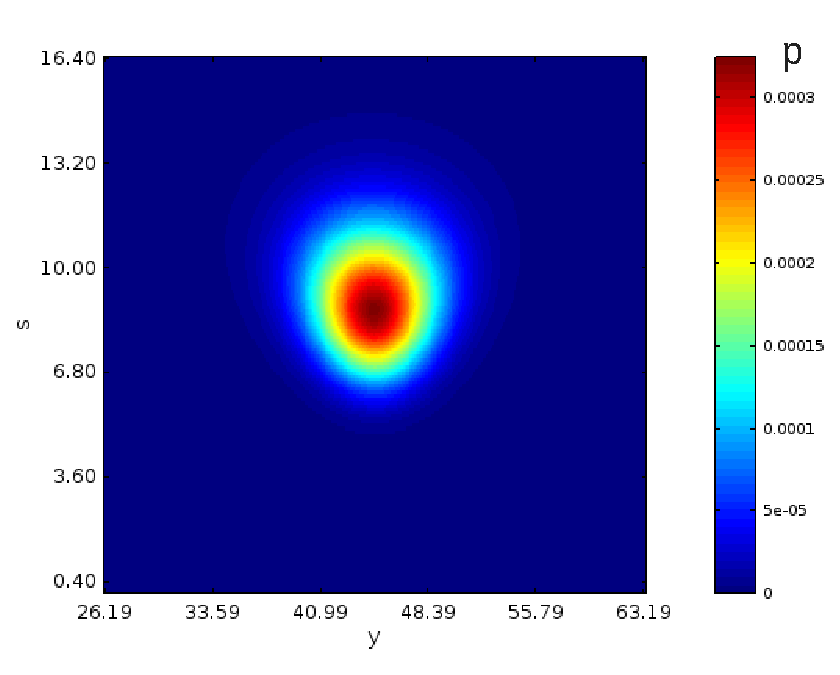
\includegraphics[width=100mm]{04_vorlesung/media/understand_bayes_mean_posteriormatrix.pdf}
\caption{\label{posteriormatrix} Posterior-Wahrscheinlichkeitsdichte als Funktion
der beiden zu schätzenden Größen $y$ und $s$.}
\end{center}
\end{figure}
Das Produkt ist die Wahrscheinlichkeit des Modellparameters und dessen Varianz gegeben
die Stichprobe $\{X_{1,1}, \dots, X_{1,J}\}$ und die {\`a} priori Informationen $y_0, s_0$
\begin{equation}
p(y, s | \{X_{1,1}, \dots, X_{1,J}\}, y_0, s_0) \; = \; C \,
p_\mathrm{L}(\{X_{1,1}, \dots, X_{1,J}\} | y, s) \; p_\mathcal{N}(y | y_0, s_0) \; p_{\chi^2,\nu}(s)
\label{ProduktWahrscheinlichkeiten}
\end{equation}
mit $C$ als Normierungsfaktor derart zu wählen, dass die integrierte Wahrscheinlichkeit Eins ist, d.h.
$$
\int\limits_{-\infty}^\infty  \int\limits_0^\infty \; p(y, s | \{X_{1,1}, \dots, X_{1,J}\}, y_0, s_0) \;
\mathrm{d}s \, \mathrm{d}y \; = \; 1 .
$$
Die Verteilungsdichte $p(y, s | \{X_{1,1}, \dots, X_{1,J}\}, y_0, s_0)$ ist Funktion der
Variablen $y$ und $s$ mit vorgegebenen Parametern 
(festen Werten) $\{X_{1,1}, \dots, X_{1,J}\}$, $y_0, s_0$, wie es beispielhaft in 
Abb.~\ref{posteriormatrix} dargestellt wird.

Die Wahrscheinlichkeitsdichteverteilung
$p_\mathcal{N}(y | y_0, s_0)$ wird \textsl{Prior} genannt und die
Wahr\-schein\-lich\-keits\-dichte\-ver\-teilung $p(y, s | \{X_{1,1}, \dots, X_{1,J}\}, y_0, s_0)$
wird \textsl{Posterior} genannt.

Wir integrieren Gl.~(\ref{ProduktWahrscheinlichkeiten}) über $s$, um eine 
Wahrscheinlichkeits\-dichte\-verteilung zu gewinnen, die nur noch Funktion von $y$ ist
\begin{equation}
p(y | \{X_{1,1}, \dots, X_{1,J}\}, y_0, s_0)  \; = \;
\int\limits_0^\infty p(y, s | \{X_{1,1}, \dots, X_{1,J}\}, y_0, s_0) \operatorname{d}s
\label{RandverteilungPosterior}
\end{equation}
Diese Verteilung wird \textsl{Randverteilung} oder \textsl{Marginalverteilung} genannt.
Allgemeiner gilt: Gegeben zwei Zufallsgrößen $A$ und $B$ mit gemeinsamer Verteilungsdichte
$p(A, B)$; dann heißen die Verteilungen der einzelnen Zufallsgrößen
$A$ und $B$ die Randverteilungen des Zufallsvektors $(A, B)$.

Als Schätzwert für $Y$ berechnen wir den Erwartungswert des Modellparameters $\mu$
durch Integration über alle Werte $y$ gewichtet mit der Wahrscheinlichkeitsdichte\\
$p(y | \{X_{1,1}, \dots, X_{1,J}\}, y_0, s_0)$ aus Gl.~(\ref{RandverteilungPosterior})
\begin{equation}
y_1 \; = \; \int\limits_{-\infty}^\infty \, y \, p(y | \{X_{1,1}, \dots, X_{1,J}\}, y_0, s_0) 
\operatorname{d}y
\end{equation}
wobei wir $y_1$ mit Index $1$ schreiben, um anzuzeigen, dass dies die Revision der Schätzung des 
Modellparameters $\mu \approx Y$ gegenüber vorheriger Kenntnis mit Schätzwert $y_0$ ist.

Zu einem \textsl{Messergebnis} gehört jeweils ein Intervall, das ein Maß für die Unsicherheit
des Wertes/ der Werte der Messgröße ist, siehe [VIM 2.9]

\begin{quote}
\textbf{Messergebnis}

Menge von Größenwerten, die einer Messgröße zugewiesen sind, zusammen mit jeglicher
verfügbarer relevanter Information

ANMERKUNG 1 Ein \textsl{Messergebnis} enthält im Allgemeinen \glqq relevante Information\grqq ~über
die Menge der Größenwerte, von denen einige repräsentativer für die Messgröße sein können als andere.
Dies kann in Form einer Wahrscheinlichkeitsdichtefunktion ausgedrückt werden.

ANMERKUNG 2 Ein \textsl{Messergebnis} wird im Allgemeinen
als ein einziger Messwert und eine \textsl{Messunsicherheit}
ausgedrückt. Wird die Messunsicherheit für einige
Zwecke als vernachlässigbar angesehen, kann das
Messergebnis als ein einziger Messwert ausgedrückt
werden. In vielen Bereichen ist dies die übliche Art, ein
Messergebnis auszudrücken.

ANMERKUNG 3 In der traditionellen Literatur und in der
vorhergehenden Ausgabe des VIM war das Messergebnis
als ein Wert definiert, der einer Messgröße zugewiesen
ist, und so erklärt, dass er eine Anzeige oder ein
unkorrigiertes oder ein korrigiertes Ergebnis bedeutet, je
nach Kontext.
\end{quote}

Mit der in Anmerkung~1 angesprochenen Wahrscheinlichkeitsdichtefunktion sind Verteilungen wie
die in den Gln.~(\ref{Likelihood2}) und (\ref{LikelihoodKov2}) vorgestellen Likelihoods oder
der in Gl.~(\ref{RandverteilungPosterior}) vorgestellten Posterior
mit $p(y | \{X_{1,1}, \dots, X_{1,J}\}, y_0, s_0)$ gemeint. Die Likelihood wird
für kleine Stich\-proben\-um\-fänge ($N < 100$) anstelle durch eine Gaußverteilung durch eine Verteilung 
repräsentiert, deren Charakteristik im Kurvenverlauf
überhöhter und mit länger auslaufenden Rändern ist. Sie wird $t$-Verteilung genannt.
Wir werden später in der 5.\ Vorlesung auf diesen Verteilungtyp zurück kommen.

Allgemein betrachten wir für beide Fälle eine Wahrscheinlichkeitsdichtefunktion $p \! : y \mapsto p(y)$.
Der Definitionsbereich für $y$ reicht von minus bis plus Unendlich. Von Interesse ist der Kernbereich
der Dichteverteilung für eine spezifizierte Wahrscheinlichkeit $1-\alpha$, beispielsweise
$1-\alpha = 0.95$ oder $0.90$ oder so.
Dies ist die Wahrscheinlichkeit einer Größe, einen Messwert im Bereich (Intervall) $[y_\mathrm{min}, y_\mathrm{max}]$,
anzunehmen
\begin{equation}
1 \, - \, \alpha \; = \; 
\int\limits_{y_\mathrm{min}}^{y_\mathrm{max}} p(y) 
\operatorname{d}y .
\label{UeberdeckungWahrscheinlichkeit}
\end{equation}
Die Breite des Intervalls gibt dann die \textsl{Messunsicherheit} an.

Das Intervall $[y_\mathrm{min}, y_\mathrm{max}]$, zu dem die Fläche $1 - \alpha$ unter der die
Verteilungsdichte $p(y)$ repräsentierenden Kurve gehört, wird \textsl{Überdeckungsintervall} genannt.
Es ist der verallgemeinerte Begriff aus der Metrologie für das, was in der
\textsl{frequentistischen} Statistik \textsl{Vertrauensintervall},
engl.\  \textsl{Confidence Interval}, und in der \textsl{bayesischen} Statistik 
\textsl{Glaubwürdigkeitsintervall}, engl.\ \textsl{Credible Interval},
heißt. Während der Begriff \textsl{Vertrauensintervall} in der deutschsprachigen
Literatur üblich ist, wird anstelle des Begriffs \textsl{Glaubwürdigkeitsintervall} üblicherweise
auch in der deutschsprachigen Literatur der Begriff \textsl{Credible Interval} verwendet.

Die Verwendung unterschiedlicher Bezeichnungen, \textsl{Confidence Interval} und
\textsl{Credible Interval}, sollen die Unterschiedlichkeit der Vorstellungen
über den Charakter einer indirekten Messgröße $Y$ zum Ausdruck bringen.
Die Unterschiedlichkeit in der Vorstellung von einer indirekten Messgröße $Y$ besteht darin,
dass im Fall der \textsl{bayesischen} Statistik
die indirekte Messgröße $Y$ als Größe, die intrinsisch eine Zufallsgröße ist, betrachtet
wird. Im Fall der \textsl{frequentistischen} Statistik wird $Y$ als eine Größe betrachtet,
die einen festen, wahren Wert hat, der aber nicht zugänglich ist. Nur der
Modellparameter, der eine indirekte Messgröße approximiert und der indirekt aus anderen 
Zufallsgrößen gewonnen wird, wird als daraus resultierend einer Streuung unterliegend betrachtet.

Die Wahrscheinlichkeit $1 - \alpha$ wird in der \textsl{frequentistischen} Statistik
\textsl{Vertrauensniveau} genannt. Die beiden Flächen unter den
Ausläufern der Dichteverteilung stellt eine Wahrscheinlichkeit $\alpha$ dar, die in der
\textsl{frequentistischen} Statistik \textsl{Signifikanzniveau} genannt wird.

Im folgenden werden wir sehen, wie eine \textsl{Messunsicherheit} im Rahmen der
\textsl{bayesischen} Statistik gewonnen wird.
Die Grenzen des \textsl{Credible Interval} $[y_\mathrm{min}, y_\mathrm{max}]$ bilden die
Integrationsgrenzen $y_\mathrm{min}$ und $y_\mathrm{max}$ der \textsl{Posterior}, so dass
\begin{equation}
1 \, - \, \alpha \; = \; 
\int\limits_{y_\mathrm{min}}^{y_\mathrm{max}} p(y | \{X_{1,1}, \dots, X_{1,J}\}, y_0, s_0) 
\operatorname{d}y .
\label{UeberdeckungPosterior}
\end{equation}
Die Integrationsgrenzen werden über die Umkehrfunktion der kumulativen Verteilung $P$ berechnet.
Die kumulative Verteilung $P$ ist
\begin{equation}
P(y) \; = \; \int\limits_{-\infty}^{y} p(y^\prime | \{X_{1,1}, \dots, X_{1,J}\}, y_0, s_0) 
\operatorname{d}y^\prime .
\end{equation}
Die Umkehrfunktion schreiben wir symbolisch als $P^{-1}$.
Wir berechnen für das \textsl{Credible Interval}
\begin{equation}
y_\mathrm{min} \, = \, P^{-1}(\frac{\alpha}{2}) \qquad \mathrm{und} \qquad
y_\mathrm{max} \, = \, P^{-1}(\frac{1-\alpha}{2}).
\end{equation}
\begin{figure}
\begin{center}
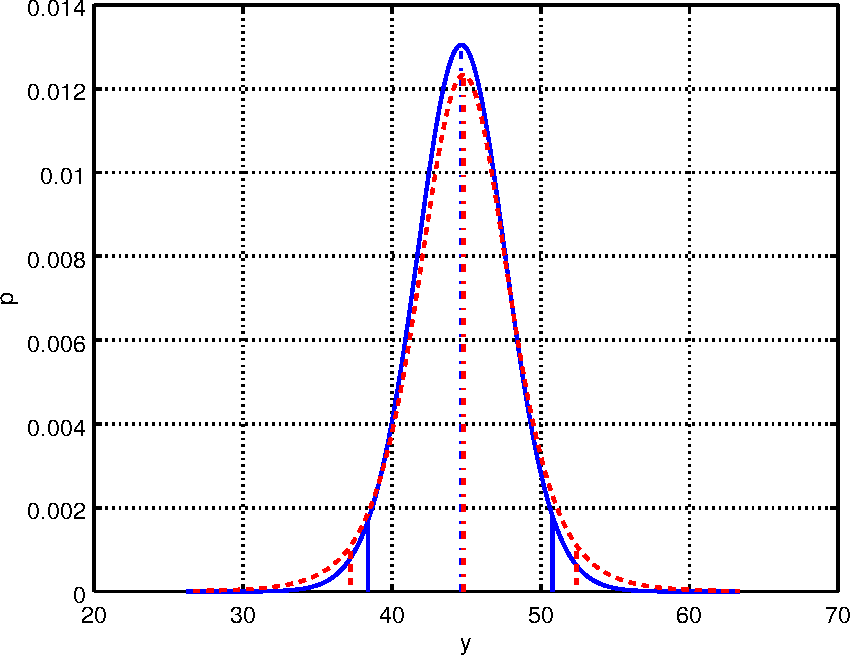
\includegraphics[width=80mm]{04_vorlesung/media/understand_bayes_mean_posteriormarginal.pdf}
\hspace{5mm}
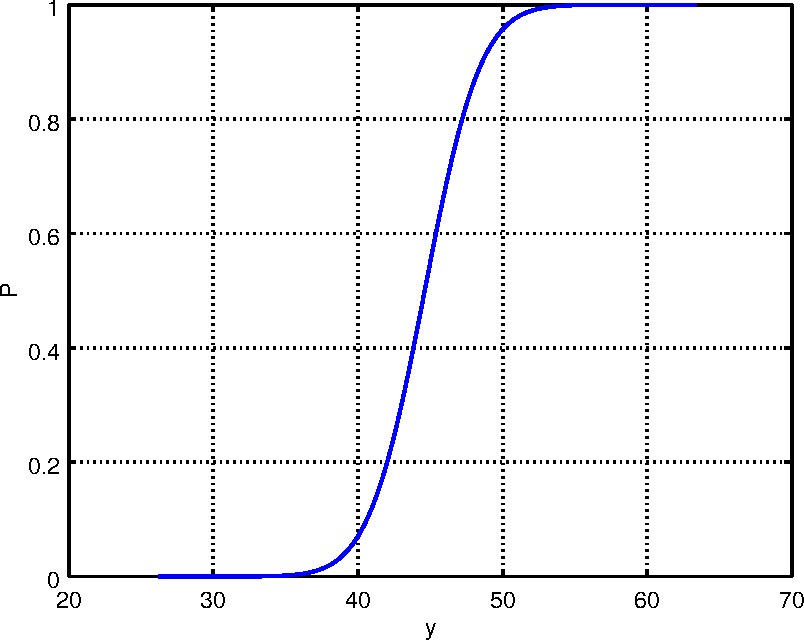
\includegraphics[width=80mm]{04_vorlesung/media/understand_bayes_mean_cumposterior.pdf}
\caption{\label{posteriorCredible}\textsl{Links:} Die blaue Kurve stellt die
Randverteilung der Posterior-Wahrscheinlichkeitsdichte als Funktion
der beiden zu schätzenden Größen $Y$ mit \textsl{Credible Interval} dar und die
rot gestrichelte Kurve die Student-t-Verteilung mit Vertrauensintervall.
\textsl{Rechts:} Kumulierte Randverteilung der Posterior-Wahrscheinlichkeitsdichte, deren
Umkehrfunktion verwendet wird, um die Intervallgrenzen des \textsl{Credible Interval}s zu ermitteln.}
\end{center}
\end{figure}
Abb.~\ref{posteriorCredible} links zeigt im Vergleich folgende Verteilungsdichten
\begin{itemize}
\item die Posterior als Funktion des Parameters
$y$ mit einem \textsl{Credible Interval} für eine Wahrscheinlichkeit von
$1 - \alpha = 0.95$ (blaue, durchgezogene Kurve und blaue, durchgezogene Linien)
\item die $t$-Verteilung (rote, gestrichelte Kurve), die sich für die in dem
graphisch dargestellten Beispiel verwendeten Stichprobe mit Stichprobenumfang $J = 7$, folglich
$\nu = J - 1 = 6$ Freiheitsgraden ergeben hat, sowie das Vertrauensintervall (rote, gestrichelte Linien),
das aus dem Mittelwert der Stichprobe
und der empirischen Standardabweichung des Mittelwerts multipliziert mit dem
t-Quantil gewonnen wurde. Mit dem Begriff t-Quantil werden die Integrationsgrenzen dieser Verteilung
zu vorgegebenen Wahrscheinlichkeiten $\frac{\alpha}{2}$ und $1 - \frac{\alpha}{2}$ bezeichnet.
\end{itemize}

Abb.~\ref{posteriorCredible} rechts zeigt die kumulierte Posterior, aus deren Umkehrfunktion
zu den Wahrscheinlichkeiten $\frac{\alpha}{2}$ und $1 - \frac{\alpha}{2}$ die
Intervallgrenzen des \textsl{Credible Interval}s gewonnen werden.

Die Ermittlung der \textsl{Messunsicherheit} im Rahmen der
\textsl{frequentistischen} Statistik unter Verwendung der $t$-Verteilung
wird in den kommenden Wochen detailiert und mit Beispielen dargelegt werden.
Sie wird einen großen Teil dieser Vorlesungsreihe ausmachen und Klausurrelevanz haben.


%
\chapter{Wahrscheinlichkeiten und Hypothesentests}

\section{Konzept der statistischen Erwartung}

Das \textsl{Signifikanzniveau} $\alpha$ und die dazu komplementäre Wahrscheinlichkeit,
das \textsl{Vertrauensniveau} $1 - \alpha$ spielen eine zentrale Rolle bei der Bewertung
von Messergebnissen. Als wir in Kapitel~\ref{KonzepteinverseProbleme} die Konzepte der statistischen Auswertung
behandelt hatten,
haben wir diese beiden Begriffe gemeinsam mit dem des \textsl{Vertrauensintervalls} bzw.\
\textsl{Credible Interval} eingeführt, mit dem gemeinsamen Oberbegriff \textsl{Überdeckungsintervall}.
Es ist das Intervall, in dem mit einer Wahrscheinlichkeit von $P(X_1) = 1 - \alpha$ die
beobachteten Werte $X_{1,j}$ zur Größe $X_1$ liegen, das also die \glqq meisten\grqq
~Beobachtungen abdeckt.

Die Idee hinter dem Begriff des \textsl{Vertrauensintervalls} oder des \textsl{Credible Interval}s
ist, dass beim Bestimmen einer physikalischen Größe $X$ eine Vorstellung (eine Erwartung) darüber
existiert, wie die gemessenen oder beobachteten Werte verteilt sind. Das schließt die
Erwartung von Position und Breite des Bereichs, in dem die Werte liegen sollten, ein.
Diese Erwartung wird quantifiziert mit einer Angabe über die Wahrscheinlichkeit, dass die
zu messende Größe diesen oder jenen Wert annimmt, eher noch in welchem Bereich (Intervall) der
Wert zu erwarten ist. Wir \textsl{vertrauen} also darauf, dass wir einen Wert messen, der innerhalb eines
gewissen Intervalls liegen müsste, oder sagen, dass es plausibel oder \textsl{glaubwürdig}
(engl.\ \textsl{credible}) ist, dass die Beobachtungen in dem Intervall liegen.
Statt zu sagen, dass wir \textsl{eine Vorstellung haben}, können wir auch sagen,
dass wir \textsl{eine Hypothese aufstellen}. 


Die Normalverteilung (Gaußverteilung) ist die grundlegende Verteilungsdichtefunktion
zur Beschreibung zufälliger Prozesse, beispielsweise Zerfallsprozesse und Diffusionsprozesse.
Bei rein stochastischen Prozessen wird von Zufallsgrößen ausgegangen, deren
Wahrscheinlichkeitsdichteverteilung eine Normalverteilung ist
\begin{equation}
p(X) \; = \; \frac{1}{\sqrt{2 \pi} \, \sigma} \, e^{-\frac{1}{2}\left(\frac{X - \mu}{\sigma}\right)^2}.
\end{equation}
Verteilungen wie die Poisson-Verteilung und die Binominal-Verteilung gehen für
unendlich viele Beobachtungen oder Stichprobenentnahmen in die Gaußverteilung über.

In der Wahrscheinlichkeitstheorie wird diese Tatsache exakt formuliert und ist der
\textsl{zentrale Grenzwertsatz} (engl.\ \textsl{central limit theorem}) CLT.
In einfacheren Worten können wir sagen:
\begin{quote}
Die Summe einer großen Anzahl von unabhängigen Zufallsgrößen folgt
asymptotisch einer stabilen Verteilung.
\end{quote}
Bei endlicher und positiver Varianz der Zufallsgrößen ist ihre Summe annähernd
normalverteilt, was die Sonderstellung der Normalverteilung erklärt.

Hierzu wird das Ziehen eines Wertes (das Machen einer Beobachtung) als Zufallsgröße
interpretiert.
Damit betrachten wir eine Stichprobe als Folge von Zufallsgrößen. Sind die Elemente
einer Stichprobe Zufallsgrößen, die
\textsl{unabhängig und identisch verteilt}, kurz u.i.v., sind, so ist auch ihre Summe
eine Zufallsgröße, die normalverteilt ist, wenn der Stichprobenumfang beliebig groß ist,
also gegen Unendlich konvergiert. In der englischsprachigen Literatur ist 
\textsl{unabhängig und identisch verteilt} unter dem Begriff
\textsl{independent and identically distributed}, kurz i.i.d., zu finden.

Liegt nun eine Einzelbeobachtung innerhalb der flachen
Ausläufer (\textsl{tails}) der Wahrscheinlichkeitsdichteverteilung,
also außerhalb des Vertrauensintervalls, so 
spricht man dann davon, dass der Wert (die Einzelbeobachtung)
signifikant von dem, was zu erwarten ist, abweicht. Das heißt, dass ein Ereignis eintritt,
das \textsl{nicht der Erwartung entspricht}. Somit \textsl{vermuten wir ein Problem}. Das Aufspüren
des Problems erfolgt durch \textsl{Hypothesentests}. Da die Normalverteilung
lange Ausläufer hat, gibt es eine kleine Wahrscheinlichkeit $\alpha$ dafür, dass es
weiter abseits liegende Werte gibt. Deshalb gilt es zu untersuchen,
ob solch ein Wert in der Tat im Rahmen der Normalverteilung weiter weg liegt
oder aber ob er auf Basis eines anderen Effektes gewonnen
wurde, ob er - statistisch formuliert - zu einer anderen Grundgesamtheit gehören könnte.

Der \textsl{Kolmogorow-Smirnow-Test} ist ein möglicher Test zum Prüfen, ob eine aus Beobachtungen
empirisch ermittelte Verteilung zu einer für die statistische Analyse der Beobachtungen
zugrundegelegten (erwarteten) Wahrscheinlichkeitsdichtefunktion passt.

% 30. Okt 2017

\section{Kolmogorow-Smirnow-Test}

\begin{figure}
\begin{center}
\includegraphics[width=80mm]{05_vorlesung/media/learn_robust.pdf}
\includegraphics[width=80mm]{05_vorlesung/media/learn_robust_2.pdf}
\caption{Beispiel für nicht erwartungsgemäße Beobachtungen (\textsl{rechts}) und
Umgewichten um die Verteilungform der Normalverteilung anzupassen \textsl{links}}
\label{biasExample}
\end{center}
\end{figure}
Das in Abb.~\ref{biasExample} dargestellte Beispiel zeigt dieselben Diagramme und
Daten, die wir in Abschnitt~\ref{robustEstimation} bereits zur Veranschaulichung
robuster Schätzverfahren behandelt hatten. Den robusten Schätzverfahren liegt die
im folgenden erläuterte statistische Betrachtung zugrunde: Es liegt eine Annahme
(Hypothese) darüber vor, welcher Gestalt die Wahrscheinlichkeitsverteilung der
Beobachtungen ist und ob ein Reihe von Beobachtung zu einer gemeinsamen Verteilung
gehören oder zu unterschiedlichen Verteilungen. Technisch gesehen stellen sich die
Fragen, die statistisch formuliert lauten \glqq gehören Beobachtungen zu einer 
Verteilung\grqq ~oder \glqq gehören Beobachtungen zu mehreren verschiedenen Verteilungen\grqq,
als 
\begin{itemize}
\item \glqq stammen die Messwerte aus einem Prozess\grqq ~oder \glqq aus unterschiedlichen
Prozessen\grqq, 
\item \glqq werden alle Messwerte von demselben Effekt beeinflusst \grqq ~oder \glqq gibt es
für verschiedene Gruppen aus der Messreihe unterschiedliche beeinflussende Effekte\grqq.
\end{itemize}
Die Annahmen bzw.\ Hypothesen bezüglich der Verteilungen zur Wahrscheinlichkeit
von Beobachtungswerten werden geprüft. Diese Art der Prüfung wird \textsl{Hypothesentest}
genannt. Es gibt unterschiedliche Typen von Hypothesentests, einer davon ist 
der \textsl{Kolmogorow-Smirnow-Test}.
Er ist ein statistischer Test auf Übereinstimmung zweier Wahrscheinlichkeitsverteilungen.

Der Test verwendet die kumulierten Wahrscheinlichkeitsfunktionen
\begin{equation}
P(X) \; = \; \int\limits_{-\infty}^X \, p(X^\prime) \, \mathrm{d} X^\prime .
\end{equation}
Das hat den Vorteil, dass
die Verteilung der empirischen Häufigkeiten ohne Histogrammierung, d.h.\ ohne Einteilung in Klassen,
erfolgen kann.

Wir wollen damit prüfen, ob die Beobachtungen des in Abschnitt~\ref{robustEstimation} zur robusten
Schätzung betrachteten Beispiels der Annahme folgt, zu der Grundgesamtheit \textsl{genau einer}
Zufallsgröße $X_1$ zu gehören. Ferner nehmen wir an, dass ihre Ausprägungen (Beobachtungswerte)
unabhängig und identisch der Normalverteilung folgen.
\begin{quote}
Die Nullhypothese lautet:\\
Die Beobachtungen zu $X_1$ gehören zu einer
normalverteilten Grundgesamtheit.
\end{quote}
Wir prüfen, ob die Stichprobe $(X_{1,1}, X_{1,2}, \dots, X_{1,J})$ bezüglich
des Mittelwertes $y \, = \, \frac{1}{J} \sum_{j=1}^J X_{1,j}$ und der
empirischen Varianz $s^2 \, = \, \frac{1}{J-1} \sum_{j=1}^J (X_{1,j} \, - \, y)^2$ normalverteilt
ist. Die kumulierte Normalverteilung, mit der wir die kumulierte Verteilung der relativen Häufigkeiten
vergleichen, ist
\begin{equation}
P(X) \; = \;  \frac{1}{\sqrt{2\pi} s} 
\int\limits_{-\infty}^X \, e^{-\frac{1}{2}\left(\frac{X^\prime \, - \, y}{s}\right)^2} \, \mathrm{d} X^\prime .
\label{cdfKS}
\end{equation}
Die kumulierte Verteilung der relativen Häufigkeiten gewinnen wir darüber, dass wir die Werte der
Stichprobe in aufsteigender Reihenfolge sortieren
\begin{equation}
X_{1,k_1} \, \leq \, X_{1,k_2} \, \leq \,  \dots \, \leq \,  X_{1,k_J}
\end{equation}
Die Teilstichprobe mit der Beobachtung mit dem kleinsten Wert $(X_{1,k_1})$ hat die
relative kumulierte Häufigkeit $\frac{1}{J}$, die Teilstichprobe mit den zwei
kleinsten Beobachtungen $(X_{1,k_1}, X_{1,k_2})$ hat die relative kumulierte Häufigkeit $\frac{2}{J}$.
Die Teilstichprobe
\begin{equation}
(X_{1,k_1}, X_{1,k_2}, \dots, X_{1,k_j})
\qquad \mathrm{die~rel.~kum.~Haeufigk.} 
\qquad H(X_{1,k_j}) \; = \; \frac{j}{J}
\label{cdfH}
\end{equation}
\begin{figure}
\begin{center}
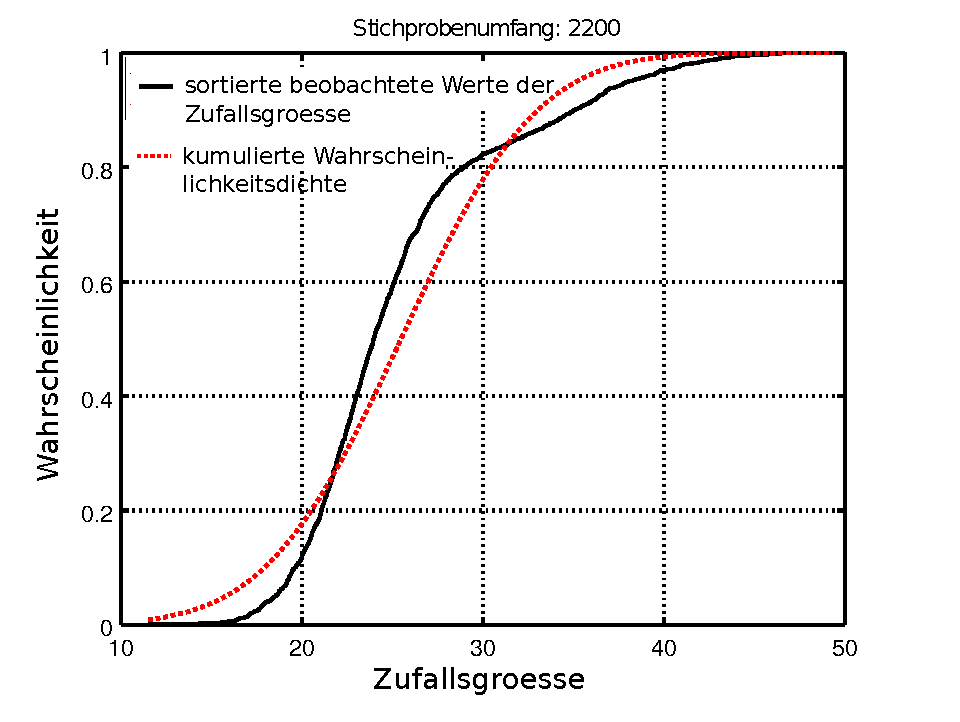
\includegraphics[width=100mm]{05_vorlesung/media/KS_pdf_iteration0.pdf}
\caption{\label{cdf4KStest} Vergleich der Wahrscheinlichkeiten (kumulierte Verteilungsdichten) aus der
empirische gewonnenen Häufigkeit der beobachteten Werte der Zufallsgröße
(schwarze, durchgezogene Kurve) mit der kumulierten Normalverteilung, die sich auf
die empirischen Erwartungswerte, den Mittelwert und die empirische Varianz, bezieht (rote,
gestrichelte Kurve).}
\end{center}
\end{figure}

Abb.~\ref{cdf4KStest} stellt zum Vergleich die Wahrscheinlichkeitsfunktion
(kumulierte Verteilungsdichte) $P(X)$ gemäß Gl.~(\ref{cdfKS})
als rote, gestrichelte Kurve und die kumulierte, relative Häufigkeit
$H(X_{1,k_j}) \; = \; \frac{j}{J}$
als schwarze, durchgezogen gezeichnete Kurve in einem Diagramm dar.


Die Prüfgröße des \textsl{Kolmogorow-Smirnow}-Tests ist
\begin{equation}
\arraycolsep=2.4pt\def\arraystretch{2}
\begin{array}{l}
\sup\limits_{X} \mid H(X_{1,k_j}) \, - \, P(X) \mid \; = \;\\
\max\limits_{k_j} \left\{ \max \left\{ \mid H(X_{1,k_j}) \, - \, P(X_{1,k_j}) \mid, \;
\lim\limits_{X \rightarrow X_{1,k_j}} \mid H(X) \, - \, P(X_{1,k_j} - 1) \mid \right\} \; \right\} .
\end{array}
\end{equation}
Dabei steht sup für Supremum, was \textsl{kleinste, obere Schranke} heißt.
Zu jeder Ausprägung der Stichprobe wird der Betrag der beiden Wahrscheinlichkeitsverteilungen
gebildet. Die Berechnung des Grenzwertes
$\lim\limits_{X \rightarrow X_{1,k_j}} \mid H(X) \, - \, P(X_{1,k_j} - 1) \mid$
für das Supremum ist erforderlich, wenn die kumulierte relative Häufigkeit
(Summenhäufigkeit) durch Kumulieren eines Histogramms, also einer in Klassen
quantisierten Stichprobe, berechnet wurde. Dabei soll die Schreibweise mit
dem Grenzwert $\lim\limits_{X \rightarrow X_{1,k_j}} \mid H(X) \, - \, P(X_{1,k_j} - 1) \mid$
zum Ausdruck bringen, dass man infinitesimal dicht aber doch prinzipiell rechts 
von $X_{1,k_j}$ an der Stufe ist, praktisch wird aber direkt
$\mid H(X_{1,k_j}) \, - \, P(X_{1,k_j} - 1) \mid$
berechnet. Für die nichtklassierte, sortierte Stichprobe berechnen wir einfach nur
\begin{equation}
\max\limits_{k_j} \left\{ \mid H(X_{1,k_j}) \, - \, P(X_{1,k_j}) \mid \right\} .
\end{equation}

Die Wahrscheinlichkeit, dass die Beobachtungen nicht zur in der Hypothese angenommenen
Verteilung passt, ist die Wahrscheinlichkeit, dass die Beobachtung
in den Ausläufern (\textsl{Tails}) der Dichteverteilung liegt, weshalb wir
die durch die Fläche in den Tails repräsentierte Wahrscheinlichkeit mit
\textsl{Signifikanzniveau} $\alpha$ bezeichnen.

Beim Kolmogorow-Smirnow-Test wird die Nullhypothese verworfen, wenn
die empirische relative Häufigkeit einen Grenzwert überschreitet,
der vom Signifikanzniveau $\alpha$ und dem Stichprobenumfang $J$ abhängt
\begin{equation}
\sup\limits_{X} \mid H(X_{1,k_j}) \, - \, P(X) \mid \; > \; K_{\alpha, J}
\end{equation}
wobei es zu Schwellwerten $K_{\alpha, J}$ für $J < 35$ Tabellen in den gängigen
Formelsammlungen gibt und
für $J \geq 35$ folgende Näherung verwendet wird:
\begin{equation}
K_{\alpha, J} \; = \; \sqrt{-\frac{1}{2 \, J} \, \ln(\frac{\alpha}{2})}
\label{KSpruefgroesse}
\end{equation}


\section{Wahrscheinlichkeitsdichtefunktionen und ihre Parameter}

Bei vielen beobachteten Stichproben, die signifikant von dem Modell, das besagt, dass sie zu genau einer
normalverteilten Grundgesamtheit gehören, abweichen, handelt
es sich um Beobachtungen aus Prozessen, denen mehrere überlagerte stochastische Anteile
zugrunde liegen. Bei dem in Abb.~\ref{biasExample} illustrierten Beispiel waren dies
zwei normalverteilte Grundgesamtheiten mit verschiedenen Erwartungswerten $\mu_1$ und
$\mu_2$ und mit unterschiedlichen Varianzen $\sigma^2_1$ und $\sigma^2_2$.

Für eine Bewertung von gemessenen Werten einer Größe, d.h.\ von Beobachtungen, werden statistische
Modelle zugrunde gelegt. Ein statistisches Modell zu beobachtbaren Größen umfasst die 
Vorstellung von Zufallsgrößen und der Verteilung ihrer Beobachtungswerte.
Wahrscheinlichkeitsdichtefunktionen werden parametrisiert über ihre statistischen Momente.
Diese charakterisieren den Kurvenverlauf der Funktion hinsichtlich ihrer Lage, Breite,
Symmetrie und so weiter.

Der \textsl{Erwartungswert einer Zufallsgröße} $X$ ist das erste statistische Moment
der Verteilungsdichte $p$ ihrer Grundgesamtheit
\begin{equation}
\mathrm{E}(X) \; = \; \int\limits_{-\infty}^{\infty} \, X \, p(X) \, \mathrm{d} X \; =: \; \mu^{(1)}(X)
\end{equation}
das ihren Schwerpunkt angibt.
Der Erwartungswert der \textsl{Varianz}
einer Zufallsgröße $X$ entspricht dem zweiten statistischen Moment
der Verteilungsdichte $p$.
Das zweite statistische Moment ist definiert durch
\begin{equation}
\int\limits_{-\infty}^{\infty} \, X^2 \, p(X) \, \operatorname{d} X \; =: \; \mu^{(2)}(X)
\end{equation}
und die Varianz ist das zweite Moment der um den Erwartungswert verschobenen Zufallsgröße
\begin{equation}
\operatorname{Var}(X) \; = \; \int\limits_{-\infty}^{\infty} \, (X - \operatorname{E}(X))^2 \,
 p(X) \, \mathrm{d} X
\end{equation}
deren Wurzel
\begin{equation}
\sigma \; = \; \sqrt{\operatorname{Var}(X)}
\end{equation}
ein Maß für die Breite von $p$ darstellt.
Die Schiefe einer Verteilungsdichte wird durch das dritte statistische Moment
\begin{equation}
\int\limits_{-\infty}^{\infty} \, X^3 \, p(X) \, \mathrm{d} X \; =: \; \mu^{(3)}(X)
\end{equation}
gewonnen, bei dem die Zufallsgröße um ihren Erwartungswert verschoben und auf die Wurzel ihrer
Varianz normiert
\begin{equation}
\operatorname{Skew}(X) \; = \; \int\limits_{-\infty}^{\infty} \, \left(\frac{X - \mathrm{E}(X)}{\sigma}
\right)^3 \, p(X) \, \operatorname{d} X
\end{equation}
wird. Das dritte statistische Moment der normierten Zufallsgröße heißt
\textsl{Skewness}.

Ein Maß für die Überhöhung oder Abflachung relativ zur Normalverteilung wird durch
das vierte statistische Moment
\begin{equation}
\int\limits_{-\infty}^{\infty} \, X^4 \, p(X) \, \mathrm{d} X \; =: \; \mu^{(4)}(X)
\end{equation}
gewonnen wird, bei dem die Zufallsgröße um ihren Erwartungswert verschoben und auf die Wurzel ihrer
Varianz normiert
\begin{equation}
\operatorname{Kurt}(X) \; = \;  \int\limits_{-\infty}^{\infty} \, \left(\frac{X - \operatorname{E}(X)}{\sigma}
\right)^4 \, p(X) \, \operatorname{d} X
\end{equation}
wird. Das vierte statistische Moment der normierten Zufallsgröße heißt
\textsl{Kurtosis}.

% ======

%Die Kombination der Wahrscheinlichkeitsverteilungen von mehreren unabhängigen kontinuierlichen
%Zufallsgrößen $X_1, \dots, X_N$ haben wir in den vergangenen Vorlesungen bereits kennengelernt,
%als wir die Berechnung der Likelihood und der Posterior besprochen haben.
%Bei der Likelihood wurde jede Beobachtung als von jeder anderen Beobachtung unabhängige
%Zufallszahl mit gleichen Varianzen (identische Verteilungen) behandelt.
%Beim Posterior wurden die Größen, zu
%denen als {`a} priori Informationen ein Erwartungswert und eine Varianz gegeben sind,
%als jeweilige Zufallsgrößen behandelt. Mit Zufallsgrößen $X_1, \dots, X_N$ können
%auch verschiedene Messgrößen sein, wie beispielsweise Strom und Widerstand (hier $N=2$),
%oder drei Koordingaten im Raum ($N=3$), oder zwei Positionskoordinaten auf einem CCD-Chip
%gemeinsam mit dem jeweiligen Intensitätswert ($N=3$).

%Gegeben seien $N$ Zufallsgrößen $X_1, \dots, X_N$ und zu jeder Zufallsgröße
%sei eine Wahrscheinlichkeitsdichteverteilung $p(X_i)$ mit $i=1,\dots,N$ gegeben.
%Dabei sei $p$ eine beliebige Verteilung. Sie muss keine Normalverteilung sein.
%Die Zufallsgrößen seinen kontinuierlich, es gelte $X_i \in I \!\! R$ und für den Zufallsvektor
%$\mathrm{X} = (X_1, \dots, X_N) \in I \!\! R^n$.
%Dann gilt unter der Voraussetzung, dass sie unabhängig voneinander sind, für die gemeinsame Wahrscheinlichkeitsdichteverteilung $p(X_1, \dots, X_N)^\mathsf{T} = p(\mathbf{X})$:
%\begin{equation}
%p(\mathrm{X}) \; = \;
%\frac{1}{\int\limits_{-\infty}^{+\infty} \dots \int\limits_{-\infty}^{+\infty}
%\prod\limits_{i=1}^N p(X_i^\prime) \mathrm{d} X_1^\prime \dots \mathrm{d} X_N^\prime}
%\prod\limits_{i=1}^N p(X_i) .
%\end{equation}
%Wir wollen uns die Verteilung für zwei Zufallsgrößen, also $\mathbf{X}^\mathsf{T} = (X_1,X_2)$,
%für den Fall, dass beide Zufallgrößen normalverteilt seien genauer anschauen
%\begin{equation}
%p(\mathbf{X}) = \frac{1}{2 \pi \sigma_1 \sigma_2} \,
%e^{-\frac{1}{2} \, 
%  \left(\frac{X_1-\mu_1}{\sigma_1}\right)^2
%  \, - \, \frac{1}{2} \,  \left(\frac{X_2-\mu_2}{\sigma_2}\right)^2}
%\end{equation}

% 6. Nov. 2017

\section{Vertrauensintervall und t-Verteilung}

Wir hatten bereits in Kapitel \ref{KonzepteinverseProbleme} angesprochen, wie
\textsl{Vertrauensintervall} $[x_1, x_2]$, Wahrscheinlichkeistdichtefunktion $p$,
\textsl{Signifikanzniveau} $\alpha$ und \textsl{Vertrauensniveau} $1-\alpha$ zusammen hängen.
Das Vertrauensintervall gibt den Bereich an, in dem ein Ereignis mit 
Wahrscheinlichkeit $1-\alpha$ beobachtet wird bzw.\ die Messgröße einen Wert in diesem Bereich
annimmt, also
\begin{equation}
\int\limits_{x_1}^{x_2} p(X) \, \operatorname{d} X \; = \; 1 - \alpha .
\end{equation}
Eine Wahrscheinlichkeitsdichteverteilung $p(X)$
wird immer so normiert, dass ihre Fläche $1$ ist:
\begin{equation}
\int\limits_{-\infty}^\infty p(X) \, \operatorname{d} X \; = \; 1
\end{equation}
Das heißt mit anderen Worten:
Unsere Größe nimmt mit Wahrscheinlichkeit $1$ irgend einen beliebigen
Wert zwischen minus und plus Unendlich an.

Auch hatten wir in Kapitel \ref{KonzepteinverseProbleme} durchgenommen, wie man aus unterschiedlichen vorliegenden
Informationen eine Wahrscheinlichkeitsdichteverteilung berechnet, um den
Erwartungswert
\begin{equation}
E(X) \; = \; \int\limits_{-\infty}^\infty \, X  p(X) \, \operatorname{d} X
\end{equation}
zu bestimmen und um aus der Umkehrfunktion $P^{-1}$ der kumulativen Verteilung
das Über\-deck\-ungs\-intervall 
\begin{equation}
[P^{-1}(\frac{\alpha}{2}), P^{-1}(1-\frac{\alpha}{2})]
\end{equation}
zu ermitteln.

Man kann zur Berechnung eines Überdeckungsintervalls
rechenzeiteffizient auf vorhandene tabellierte Werte für
die Umkehrfunktion der Normalverteilung zurück greifen, wenn
folgendes der Fall ist:
\begin{itemize}
\item Über die reinen Beobachtungen $X_{1,j}$ hinaus liegen keine
Informationen vor, also keine vorherigen Ergebnisse zu den zu
schätzenden Modellparameter (kein \textsl{Prior})
und keine weiteren beeinflussenden Verteilungen. 
\item Es kann davon ausgegangen werden, dass die Streuung der
einzelnen Beobachtungswerte um das Modell
normalverteilt sind.
\end{itemize}
Für kleine
Stichprobenumfänge wird eine der Normalverteilung ähnliche Verteilung
herangezogen, die je kleiner der Stichprobenumfang ist, um so stärker ausgeprägte
Ausläufer (\textsl{Tails}) hat, die $t$-Verteilung. Diese werden wir im Laufe
dieses Kapitels beleuchten.

Zunächst erörtern wir die Berechnung der Vertrauensintervalle auf Basis
tabellierter Werte von Integrationsgrenzen zu ausgesuchten Ver\-trauens\-niveaus
der Normalverteilung. Eine solche Integrationsgrenze wird \textsl{Quantil}
genannt. Die Tabellen beziehen sich auf normierte Zufallsgrößen.
Für die Gaußverteilung normieren wir die Zufallsgröße, so dass der
Erwartungswert $\mu = 0$ ist und die Varianz $\sigma^2 = 1$, d.h.
$Z$ ist \textsl{standardnormalverteilt}
\begin{equation}
Z \; \sim \; \mathcal{N}(0,1) .
\label{standardNormalverteilt}
\end{equation}
Die Wahrscheinlichkeitsdichtefunktion $p(Z)$ ist die \textsl{Standard}normalverteilung 
\begin{equation}
p(Z) \; = \; \frac{1}{\sqrt{2 \pi}} \, e^{-\frac{1}{2} Z^2}
\qquad \textrm{mit} \qquad Z \; = \; \frac{X - \mu}{\sigma} .
\end{equation}

Die in den Formelsammlungen und Tabellenwerken aufgelisteten Grenzen sind
als obere Integrationsgrenze definiert
\begin{equation}
\int\limits_{-\infty}^{z_\alpha} p(Z) \mathrm{d} Z \; = \; \alpha .
\label{WahrscheinlichkeitQuantil}
\end{equation}
In Abb.~\ref{normVertQuantil} wird dies anhand des Quantils $z_\alpha = 0.5244$ 
zu $\alpha = 0.7$ also $70 \%$ Wahrscheinlichkeit beispielhaft gezeigt.

\begin{figure}
\begin{center}
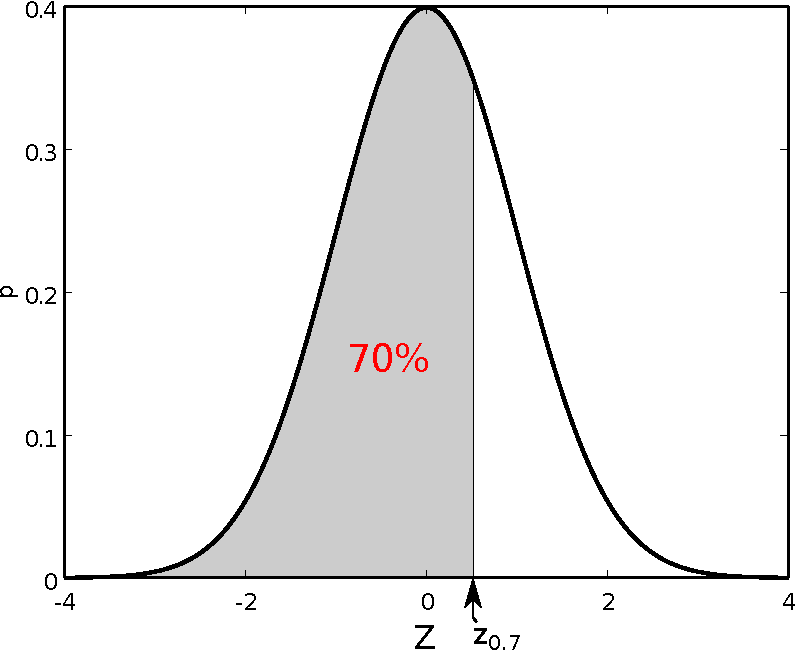
\includegraphics[width=79mm]{05_vorlesung/media/normpdfQuantil.pdf}
\hspace{5mm}
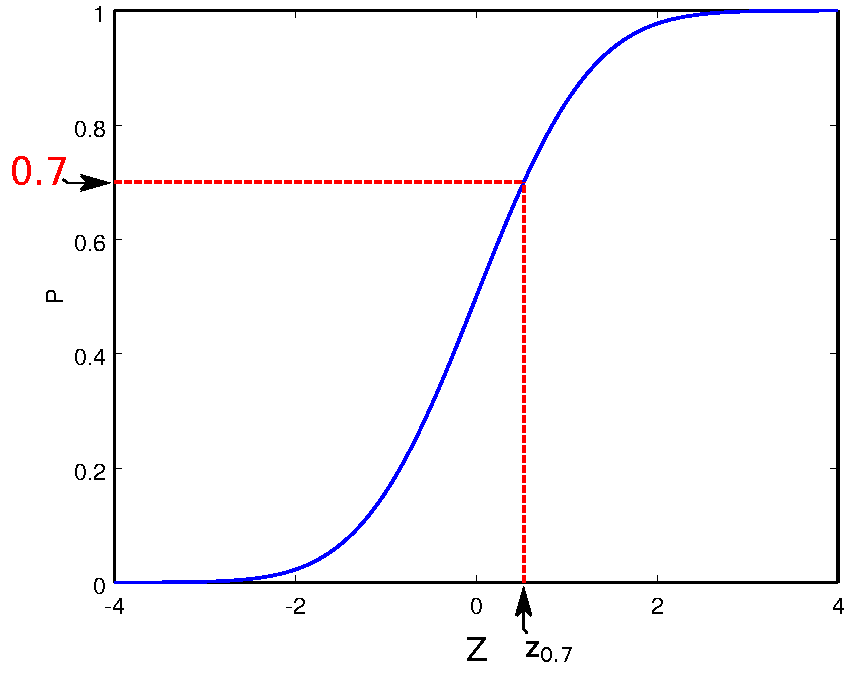
\includegraphics[width=81mm]{05_vorlesung/media/normcdfQuantil.pdf}
\caption{\label{normVertQuantil} Quantil $z_\alpha = 0.5244$ und Wahrscheinlichkeit 
$\alpha = 0.7$ der Standard\-normalverteilung.}
\end{center}
\end{figure}

Dies lesen wir so:
\begin{quote}
Die Ereignisse Werte zu $Z$ zu beobachten, die kleiner sind als $z_\alpha$, können
mit einer Wahrscheinlichkeit von $\alpha$ eintreten.
\end{quote}
Die in den Tabellenwerken gelisteten Wahrscheinlichkeiten $\alpha$ werden
aus der Integration der Wahrscheinlichkeitsdichte der normierten Zufallsgröße
von minus Unendlich bis zu einer endlichen oberen Integrationsgrenze $z_\alpha$
gewonnen.
Die zu einem Wert eines Quantils gehörende Wahrscheinlichkeit wird durch den tiefgestellten
Index bei $z_\alpha$ gekennzeichnet, in unserem Beispiel aus Abb.~\ref{normVertQuantil}
ist dies dann
$$
z_{0.7} \; = \; 0.5244
$$
Als weiteres Beispiel betrachten wir die Frage, wie hoch die Wahrscheinlichkeit ist,
Werte zu beobachten, die in den Ausläufern einer Verteilungsdichte liegen.
Die Ausläufer werden im Englischen
als \textsl{Tails} (Schwänze) bezeichnet. Dies sollen Beobachtungen zu der normierten
Zufallsgröße $Z$ mit Werten, die zum einen kleiner oder gleich $-1.960$ sind, sein
$$
z_{0.025} \; = \; -1.960
$$
und zum anderen, die Beobachtungen mit Werten größer oder gleich $1.960$, also die
in dem rechten Ausläufer (\textsl{Tail}) der Standardnormalverteilung liegen.
Die Wahrscheinlichkeit für Beobachtungen im linken \textsl{Tail} ist
\begin{equation*}
\int\limits_{-\infty}^{-1.960} p(Z) \mathrm{d} Z \; = \; 0.025 .
\end{equation*}

Aufgrund der Symmetrie der Standardnormalverteilung ist die Wahrscheinlichkeit für das Liegen von
Werten im rechten \textsl{Tail} ebenfalls $0.025$. Wir rechnen also zusammen, dass mit
einer Wahrscheinlichkeit von $0.05 = 0.025+0.025$ Werte in den beiden \textsl{Tails} außerhalb
des Intervalls $[-1.960, 1.960]$ liegen können. Somit ist die Wahrscheinlichkeit, dass sie
innerhalb des Intervalls liegen $1 - 0.05 = 0.95$
\begin{equation}
\int\limits_{-1.96}^{1.96} \, p(Z) \, \operatorname{d} Z \; = \; 0.95
\end{equation}
was uns zeigt, wie wir die Tabellen zu verwenden haben.
Wenn wir ein zweiseitiges Intervall betrachten wollen, wie hier zu einem Vertrauensniveau
von $95 \%$, so müssen wir im Tabellenwerk nach dem Quantil, das für $97.5 \%$ gelistet
ist, schauen
$$
z_{0.975} \; = \; 1.960
$$
weil
$$
0.95 \; = \; 
\underbrace{\int\limits_{-\infty}^{z_{0.975}} \, p(Z) \, \operatorname{d} Z}_{0.975} \; - \;
\underbrace{\int\limits_{-\infty}^{z_{0.025}} \, p(Z) \, \operatorname{d} Z}_{0.025}
$$
Aufgrund der Achssymmetrie der Normalverteilung gilt 
$$
z_{\frac{1}{2}\alpha} = -z_{1-\frac{1}{2}\alpha} .
$$
Da sich die Quantile zum jeweiligen Vertrauensniveau $1-\alpha$ auf die normierte Zufallsgröße
beziehen, muss für die Berechnung des Vertrauensintervall zurückgerechnet werden
\begin{equation}
Z \; = \; \frac{X - \mu}{\sigma} \qquad \Leftrightarrow \qquad X \; = \; \mu + Z \sigma
\end{equation}
also
\begin{equation}
[z_{\frac{1}{2}\alpha}, z_{1-\frac{1}{2}\alpha}] = 
[-z_{1-\frac{1}{2}\alpha}, z_{1-\frac{1}{2}\alpha}]
 \qquad \Leftrightarrow  \qquad
[\mu \, - \, z_{1-\frac{1}{2}\alpha} \, \sigma, \mu \, + \, z_{1-\frac{1}{2}\alpha} \, \sigma]
\end{equation}
Mit $\alpha$ sind die $5 \%$ und mit $1-\alpha$ die $95 \%$ Vertrauensniveau gemeint.

Die Likelihood wird maximal für
\begin{equation}
y \; = \; \frac{1}{J} \sum_{j=1}^J X_{1,j} ,
\end{equation}
wobei $y$ der Schätzwert für den Modellparameter $Y$ ist.
Der Schätzwert $s^2$ für die Varianz $\sigma^2$ wird berechnet mit
\begin{equation}
s^2 \; = \; \frac{1}{J-1} \sum_{j=1}^J (X_{1,j} - y)^2 .
\end{equation}

Nachdem wir gesehen haben, wie wir für eine normalverteilte Zufallsgröße
das Vertrauensintervall ermitteln können, wenden wir uns jetzt der Thematik zu,
wenn wir zu einer Zufallsgröße nur relativ wenige Beobachtungen haben.

%------------------- kleine Stichprobenumfaenge -> Motivation t-Verteilung
\begin{figure}
\begin{center}
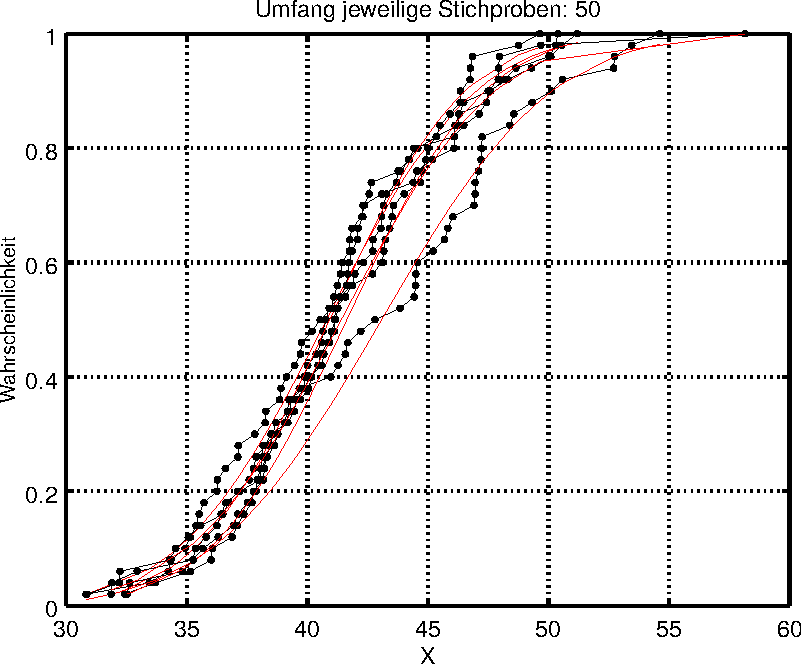
\includegraphics[width=100mm]{05_vorlesung/media/learn_Student_t1samples.pdf}
\caption{\label{kumulWahrsch} Kumulative relative Wahrscheinlichkeitsfunktionen und relative
Summenhäufigkeiten von verschiedenen Stichproben mit jeweils $J \, = \ 50$ Werten, entnommen aus einer
Grundgesamtheit mit $\mu \, = \, 42$ und $\sigma \, = \, 5$.}
\end{center}
\end{figure}
Wenn wir aus einer sehr großen Stichprobe, die einer Grundgesamtheit entnommen wurde,
disjunkte Teilstichproben von kleinerem Umfang ($J < 100$) in Grüppchen unterteilen, so können wir
beobachten, dass sowohl die Mittelwerte streuen als auch die Varianzen.
Diese Grüppchen oder Teilstichproben können wir als mehrere Stichproben aus einer normalverteilten
Grundgesamtheit ansehen. 
Abb.~\ref{kumulWahrsch} illustriert wie unterschiedlich die Verteilungsfunktionen von
Stichproben mit relativ kleinem Umfang ($J \, = \ 50$) aussehen können, obwohl sie zu derselben
Grundgesamtheit gehören. Dieses Beispiel wurde wie folgt mit Gnu-octave generiert:
\begin{verbatim}
function example_t()
  J1 = 50;
  mu1 = 42;
  sigma1 = 5;
  samples = [];
  for kappa = 1:5
    samples = [samples  (mu1 + sigma1*randn(J1,1))];
  end
  figure(3000); hold on;
  [J1, nS] = size(samples);
  for kappa = 1:5
    [P, H, xsort, xbar, s] = cumulatives(samples(:,kappa));
    plot( xsort, H, 'k.-');
    plot( xsort, P, 'r-');
  end
  xlabel('X', 'fontsize', 14);
  ylabel('Wahrscheinlichkeit', 'fontsize', 12);
  title(['Umfang jeweilige Stichproben: ' num2str(J1)], 'fontsize', 14);
  grid on;
  set(gca, 'fontsize', 14, 'linewidth', 2);
  hold off;
end
function [P, H, xsort, xbar, s] = cumulatives(x)
  xbar = mean(x);
  s = std(x);
  J1 = length(x);
  [xsort, isort] = sort(x, 'ascend');
  H = [1:J1]'/J1;
  P = normcdf( xsort, xbar, s);
end
\end{verbatim}
Zur Bewertung der Flachheit bzw.\ Ausgeprägtheit der Ausläufer einer Verteilung berechnen wir
ihre \textsl{Kurtosis}. Die \textsl{Kurtosis} der Normalverteilung hat den Wert $3$. 

Die empirischen Schätzer für den Erwartungswert, die Varianz, die Skewness und Kurtosis
berechnen wir aus einer Stichprobe mit Beobachtungswerten $X_{1,1}, \dots, X_{1,J}$
wie folgt:
\begin{itemize}
\item[] Der Mittelwert wird berechnet mit
\begin{equation}
y \; = \; \frac{1}{J}\sum_{j=1}^J \, X_{1,j} .
\end{equation}
\item[] Die empirische Standardabweichung wird berechnet mit
\begin{equation}
s \; = \; \sqrt{ \frac{1}{J-1}\sum_{j=1}^J \, (X_{1,j} - y)^2 }.
\label{empirischeStd}
\end{equation}
Zu bemerken ist, dass jetzt durch $J-1$ und nicht durch $J$ geteilt wird, weil
das $y$ aus den Werten der Stichprobe $X_{1,1}, \dots, X_{1,J}$ gewonnen wurde und somit
die Anzahl der Freiheitsgrade $\nu$ um Eins verringert wird, also $\nu = J-1$.
\item[] 
Die empirische Skewness wird berechnet mit
\begin{equation}
\textrm{skew} \; = \; \frac{1}{J} \sum_{j=1}^J \, \left( \frac{X_{1,j} - y}{s} \right)^3 .
\end{equation}
\item[] Die empirische Kurtosis wird berechnet mit
\begin{equation}
\textrm{kurt} \; = \; \frac{1}{J} \sum_{j=1}^J \, \left( \frac{X_{1,j} - y}{s} \right)^4 .
\end{equation}
\end{itemize}
Bei dem in Abb.~\ref{kumulWahrsch} gezeigten Beispiel mit mehreren Stichprobenentnahmen aus
einer Grundgesamtheit erhalten wir folgende aus den Momenten abgeleiteten empirischen 
Parameter der Verteilungen:
\begin{center}
Tabelle 1:

\begin{tabular}{c||c|c|c|c}
\hline
\multicolumn{5}{c}{Einzelstichproben, Umfang jeweils $J = 50$}\\
\hline
ltd.\ Nr. & $y$ & $s$ & skew & kurt\\
\hline\hline
1 & 40.79 &  4.83 &  0.33 &  2.50 \\
2 & 43.08 &  5.52 &  0.16 &  2.16 \\
3 & 40.92 &  4.38 & -0.26 &  2.57 \\
4 & 41.64 &  4.46 &  0.09 &  2.44 \\
5 & 41.41 &  4.98 &  0.59 &  4.16 \\
\hline\hline
\multicolumn{5}{c}{alle Stichproben zusammen, Umfang $J = 5 \cdot 50 = 250$}\\
\hline
 & 41.57 &  4.88 &  0.28 &  2.89 \\
\hline\hline
\multicolumn{5}{c}{wahre Grundgesamtheit}\\
\hline
 & $\mu$ & $\sigma$ & Skew & Kurt\\
\hline\hline
Normalvert. & 42.00 &  5.00 &  0.00 &  3.00 \\
\hline
\end{tabular}
\end{center}
%--------------------- Ende der Motivation fuer t-Verteilung

%==========
%Bei einer Überlagerung unterschiedlicher Prozesse, wie dies beispielsweise
%bei exponetiell verlaufenden Zerfällen (aus der Biologie oder Strahlenphysik) der Fall ist, sind die
%Verteilungen asymmetrisch und können z.B.\ mit einer Poissonverteilung beschrieben werden.

Man kann der Beschreibung einer kleinen Stichprobe besser gerecht werden, wenn die
Verteilung flacher ist als eine Standardnormalverteilung. Das bedeutet, dass ihre Ausläufer
ausgeprägter sind. 
Eine Verteilungsdichtefunktion, die der Gaußverteilung ähnlich ist, aber unter
Berücksichtigung des begrenzten Stichprobenumfangs entsprechend ausgeprägtere Tails hat,
ist die im folgenden dargestellte \textsl{Student-t}-Verteilung, kurz auch
einfach $t$-Verteilung genannt.

%==================

%-----------------
Diese Wahrscheinlichkeitsdichteverteilung wurde anfang des 20. Jahrhunderts von
William Sealy Gosset entwickelt. Sie wird der
Tatsache gerecht, dass die Varianz zunimmt mit kleiner werdendem Stichprobenumfang.
Gosset veröffentlichte 1908 erstmals zu dem Thema während er als Chemiker für die Guinness-Brauerei
in Dublin arbeitete. Er entwickelte einen Test zum Vergleich von Mittelwerten
einzelner Stichproben als eine billige Art und Weise, die Qualität des Stout
zu überwachen. Dieser Test wird entsprechend der zugrunde gelegten Wahrscheinlichkeitsdichtefunktion
$t$-Test genannt.
Da sein Arbeitgeber die Veröffentlichung nicht gestattete, veröffentlichte Gosset sie unter
dem Pseudonym Student. Die zugehörige Theorie wurde erst durch die
Arbeiten von R. A. Fisher belegt, der die Verteilung \textsl{Student}-Verteilung (engl.\
\textsl{Student's distribution}) nannte.

Die $t$-Verteilung bezieht sich auf eine standardnormalverteilte Zufallsgröße $Z$ und sieht wie folgt aus
\begin{equation}
p_{\nu}(Z) \; = \; 
{\frac {\Gamma \left({\frac {\nu+1}{2}}\right)}{{\sqrt {\nu \pi }} \;
\Gamma \left({\frac {\nu}{2}}\right)}} \, \left(1+{\frac {Z^2}{\nu}}\right)^{-{\frac {\nu+1}{2}}} ,
\end{equation}
wobei $\nu$ die Anzahl der Freiheitsgrade ist (was für den Fall, dass $Z$
die Summe der Stichprobenelemente darstellt, um den Mittelwert der Stichprobe mit Umfang $J$ 
zu repräsentieren, dann $\nu = J-1$ ist), und wobei
die Gamma-Funktion für natürliche Zahlen $\nu \, \in I \!\! N$ dividiert durch Zwei
wie folgt definiert ist:
\begin{equation}
\Gamma \left({\frac{\nu}{2}}\right) \; = \;
\sqrt{\pi} \, \frac{(\nu-2)!!}{ 2^{\frac{\nu-1}{2}} } \qquad \nu \, \in I \!\! N
\label{GammaHalfInt}
\end{equation}
mit $\nu!! = \nu (\nu-2) (\nu-4) \dots 4 \cdot 2$.
Wir werden auf den theoretischen Hintergrund aus der Wahrscheinlichkeitstheorie nicht
genau eingehen, also ist die Definition dieser Verteilung auch kein Klausurstoff.
Für die Klausur werden die dazugehörigen Quantiltabellen zur Verfügung gestellt, d.h.\
den Aufgabenstellungen beigefügt.

Je kleiner der Stichprobenumfang ist desto flacher wird die Verteilung, mit entsprechend
längeren Ausläufern, \textsl{Tails}, siehe
Abb.~\ref{studentt}.
\begin{figure}
\begin{center}
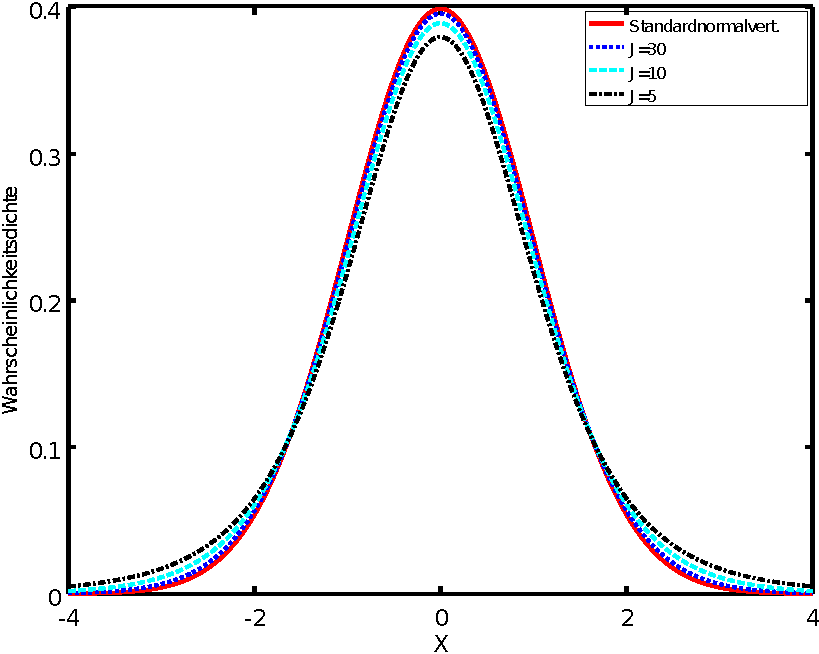
\includegraphics[width=100mm]{05_vorlesung/media/learn_Student_tpdf.pdf}
\caption{\label{studentt} Student-t Verteilungen für unterschiedliche Stichprobenumfänge.}
\end{center}
\end{figure}
Um zu verdeutlichen, wie sich die Gaußverteilung und die Student-t-Verteilung hinsichtlich
Breite und lange Ausläufer unterscheiden, haben wir hier dies im Vergleich berechnet.
Dabei haben wir bewusst ganz extrem wenig Freiheitsgrade gewählt, nämlich nur $5$.
Wir verwenden jetzt mal den empirischen Mittelwert und die empirische Standardabweichung,
die wir aus der Gesamtheit aller Stichproben gewonnen hatten, also $y = 41.57$
und $s = 4.88$. Daraus rechnen wir sowohl die Normalverteilung als auch die
Student-t-Verteilung für nur fünf Freiheitsgrade und erhalten eine größere Standardabweichung
und eine größere Kurtosis aus der Student-t-Verteilung:
\begin{center}
\begin{tabular}{l||c|c}
\hline
Verteilung & $\sigma$ & Kurt\\
\hline
Gauß &   4.88 &  2.99 \\
Student-t &  5.86 &  3.59 \\
\hline
\end{tabular}
\end{center}
Dementsprechend sind auch die Quantile größer.


Die Kurtosis
der Student-t Verteilungen nimmt Werte an, die um so größer werden, je flacher die Verteilungsdichte
ist, also je ausgeprägter die \textsl{Tails} sind, also je kleiner die Stichprobenumfänge bzw.\ die 
Anzahl der Freiheitsgrade sind.

%----

Das Vertrauensintervall zu einem Vertrauensniveau von $1 - \alpha$ für eine endlich große
Strichprobe mit Stichprobenumfang $J$ schätzen wir mit dem Quantil der Student-t-Verteilung ab.
Die Anzahl der Freiheitsgrade entspricht dem Stichprobenumfang abzüglich der Anzahl der zu
schätzenden Modellparameter, was in diesem Fall einer ist, also $\nu = J - 1$.



%---------------

Während für die Standardnormalverteilung das Quantil $z_{0.975} \; = \; 1.96$ beträgt, haben
wir aus der Student-t-Verteilung zu demselben Vertrauensniveau für $\nu = 50$ Freiheitsgrade
$t_{0.975, 50} \; = \; 2.01$ und für $\nu = 5$ Freiheitsgrade $t_{0.975, 5} \; = \; 2.57$.

\begin{figure}
\begin{center}
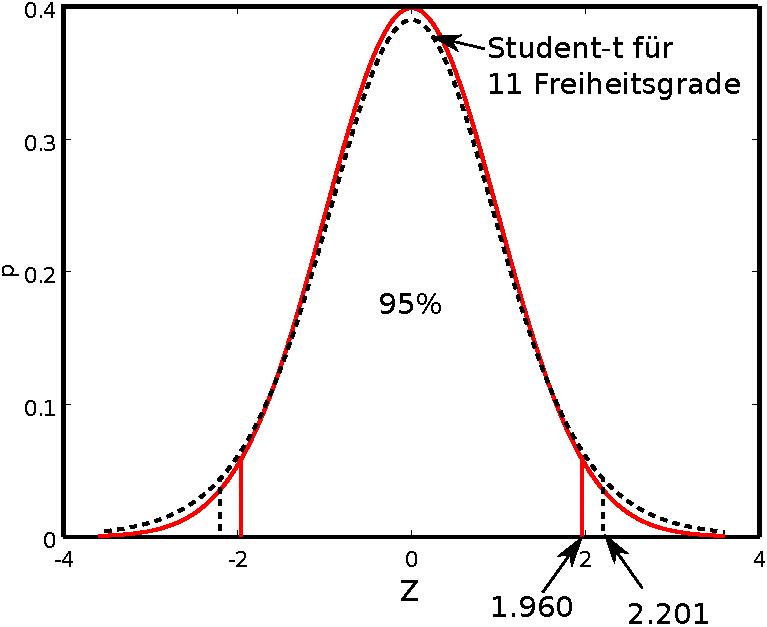
\includegraphics[width=100mm]{05_vorlesung/media/vertrauensintervall_nu_11.pdf}
\caption{\label{Vertrauensintervalle} Vertrauensintervalle in Vergleich für die 
Standardnormalverteilung (rote Kurve)
und die Student-t-Verteilung für $\nu = 11$ Freiheitsgrade (schwarze gestrichelte Kurve).}
\end{center}
\end{figure}
Für das zweiseitige, symmetrische Intervall verwenden wir das Quantil $t_{1-\alpha/2,\nu}$, so dass
wir folgendes Vertrauensintervall erhalten:
$$
[y - t_{1-\alpha/2,\nu} s, y + t_{1-\alpha/2,\nu} s]
$$
Die Breite wird durch die Anzahl der Freiheitgrade beeinflusst, je kleiner
die Anzahl der Freiheitsgrade ist, desto breiter wird das Intervall. Die beiden Abbn.~\ref{studentt}
und \ref{Vertrauensintervalle}
zeigen, dass die \textsl{Tails} einer Student-t-Verteilung für wenige Freiheitsgrade
deutlich breiter sind als bei der Standardnormalverteilung, folglich auch das
Vertrauensintervall breiter ist. In Abb.~\ref{Vertrauensintervalle} sind die Quantile für
ein Vertrauensniveau von $1 - \alpha = 0.95$ eingezeichnet.

Das \textsl{(vollständige) Messergebnis} geben wir an als
Schätzwert zur Größe $Y$ gemeinsam mit dem Vertrauensintervall.
Eine gebräuchliche Schreibweise ist
\begin{equation}
Y \; = \; y \, \pm \, t_{1-\alpha/2,\nu} s .
\label{vollstaendigesErgebKlassisch}
\end{equation}

Als nächstes befassen wir uns damit, das Vertrauensintervall des Mittelwertes abzuschätzen.
Dazu betrachten wir ein Beispiel, bei dem aus einer Grundgesamtheit mit den wahren
Werten $Y = 42$ und $\sigma = 7$ mehrere Stichproben genommen werden, beispielsweise $K = 15$,
wobei jede Stichprobe einen Umfang von $J = 25$ habe. Zu jeder der Stichproben $k = 1\dots K$
berechnen wir den Mittelwert $y_k$ und die empirische Standardabweichung $s_k$.

\begin{tabular}{c||c|c|c|c|c|c|c|c}
$k$   &  1     &    2   &    3   &   4    &    5   &   6    &   7    &   8   \\
\hline\hline
$y_k$ & 41.813 & 41.854 & 39.084 & 42.117 & 41.532 & 40.428 & 42.717 & 39.727\\
\hline
$s_k$ &  6.476 &  7.706 &  6.996 &  7.729 &  6.431 &  7.516 &  7.505 &  7.439\\
\end{tabular}

\vspace{3mm}

\begin{tabular}{c||c|c|c|c|c|c|c}
$k$   &  9     &    10  &   11   &   12   &   13   &   14   &   15  \\
\hline\hline
$y_k$ & 40.858 & 39.670 & 44.351 & 42.011 & 41.935 & 44.509 & 39.921\\
\hline
$s_k$ &  8.568 &  7.649 &  6.082 &  7.661 &  7.084 &  7.878 &  7.084\\
\end{tabular}

Der Mittelwert $\bar y$ der Mittelwerte liefert dann
$$
\bar y \; = \; \frac{1}{K} \sum\limits_{k=1}^K y_k \; = \; 41.502
$$
und die empirische Standardabweichung der Mittelwerte $y_k$ liefert
$$
\bar s \; = \; \sqrt{\frac{1}{K-1} \sum\limits_{k=1}^K (y_k \, - \, \bar y)^2 }
 \; = \; 1.606
$$
Das wiederholte Ziehen von Stichproben kann für so manche Anwendung kostspielig sein,
so dass es gilt die empirische Standardabweichung des Mittelwerts aus nur einer
Stichprobe abzuschätzen.
Dazu betrachten wir die Likelihood 
\begin{equation}
l(Y, \sigma | \{X_{1,1}, \dots, X_{1,J}\}) \; = \;
\prod\limits_{j=1}^J \frac{1}{\sqrt{2 \pi} \, \sigma}
 e^{- \frac{1}{2} \, \left( \frac{(X_{1,j} - Y)}{\sigma} \right)^2 } 
\label{LikelihoodY}
\end{equation}
und
setzten den Schätzer $y$ der Größe $Y$ als nahrhafte Null ein
\begin{equation}
l(Y, \sigma | \{X_{1,1}, \dots, X_{1,J}\}) \; = \;
\prod\limits_{j=1}^J \frac{1}{\sqrt{2 \pi} \, \sigma}
 e^{- \frac{1}{2} \, \left( \frac{(X_{1,j} - y) - (Y - y)}{\sigma} \right)^2 } 
\label{LikelihoodNahrhafteNull}
\end{equation}
d.h.
\begin{equation}
l(Y, \sigma | \{X_{1,1}, \dots, X_{1,J}\}) \; = \;
 \frac{1}{(\sqrt{2 \pi} \, \sigma)^J}
 e^{- \frac{1}{2} \, \sum\limits_{j=1}^J \left( \frac{(X_{1,j} - y) - (Y - y)}{\sigma} \right)^2 } .
\end{equation}
mit folgender Nebenrechnung für die Summe im Exponenten
$$
\arraycolsep=2.4pt\def\arraystretch{2}
\begin{array}{ll}
\sum\limits_{j=1}^J \left( (X_{1,j} - y) - (Y - y) \right)^2  & =
\sum\limits_{j=1}^J \left( (X_{1,j} - y)^2 + (Y - y)^2 - 2 (X_{1,j} - y) (Y - y) \right) \\
 & = \left( \sum\limits_{j=1}^J  (Y - y)^2\right) + 
 \left( \sum\limits_{j=1}^J  (X_{1,j} - y)^2\right) - 2 \sum\limits_{j=1}^J (X_{1,j} - y) (Y - y)\\
 & = J (Y - y)^2 + 
 \left( \sum\limits_{j=1}^J  (X_{1,j} - y)^2\right)
\end{array}
$$
und $\sum\limits_{j=1}^J (X_{1,j} - y) (Y - y) = 0$ wegen $J y = \sum\limits_{j=1}^J X_{1,j}$
gilt für die Likelihood folgende Proportionalität
\begin{equation}
l(Y, \sigma | \{X_{1,1}, \dots, X_{1,J}\}) \; \propto \;
 e^{- \frac{1}{2} \, J \, \left( \frac{(Y - y)}{\sigma} \right)^2 }
\label{LikelihoodmitJ}
\end{equation}
und wir definieren folgende Größe
\begin{equation}
\bar \sigma^2 \; := \; \frac{\sigma^2}{J}
\label{VarianzMittelwert}
\end{equation}
als \textsl{Varianz des Mittelwertes}.

Damit lässt sich Gl.~(\ref{LikelihoodmitJ}) umschreiben in
\begin{equation}
l(Y, \sigma | \{X_{1,1}, \dots, X_{1,J}\}) \; \propto \;
 e^{- \frac{1}{2} \, \left( \frac{(Y - y)}{\bar \sigma} \right)^2 } .
\end{equation}
Nun setzen wir in die Definitionsgleichung
der Varianz des Mittelwertes Gl.~(\ref{VarianzMittelwert}) bzw.\
die Wurzel daraus die empirisch ermittelten Werte unseres Beispiels ein:
\begin{equation}
\bar s \; = \; \frac{s}{\sqrt{J}}
\label{empirischeVarianzMittelwert}
\end{equation}

\begin{tabular}{c||c|c|c|c|c|c|c|c}
$k$   &  1     &    2   &    3   &   4    &    5   &   6    &   7    &   8   \\
\hline\hline
$\bar s_k$ &  1.295 &  1.541 &  1.399 &  1.546 &  1.286 &  1.503 &  1.501 &  1.488\\
\end{tabular}

\vspace{3mm}

\begin{tabular}{c||c|c|c|c|c|c|c}
$k$   &  9     &    10  &   11   &   12   &   13   &   14   &   15  \\
\hline\hline
$\bar s_k$ &  1.714 &  1.530 &  1.216 &  1.532 &  1.417 &  1.576 &  1.417\\
\end{tabular}

Jede einzelne Stichprobe liefert eine etwas unterschiedliche Abschätzung für die
Standardabweichung des Mittelwertes. Die Werte für $\bar s$ liegen mit $1.3$ bis $1.5$
knapp unter $1.6$. Es wird die Standardabweichung des Mittelwertes leicht unterschätzt, weil
der einzelne Stichprobenumfang mit $J = 25$ größer ist als die Anzahl der Stichproben mit
$K = 15$.

Das \textsl{Vertrauensintervall für die Schätzung des Mittelwertes} im Gegensatz zur
Schätzung des Einzelwertes ist damit
$$
[y - t_{1-\alpha/2,\nu} \bar s, y + t_{1-\alpha/2,\nu} \bar s]
$$
und in der Schreibweise als \textsl{vollständiges Messergebnis}
\begin{equation}
Y \; = \; y \, \pm \, t_{1-\alpha/2,\nu} \bar s .
\label{vollstaendigesErgebMittelwert}
\end{equation}


%===============


\section{t-Test - Mittelwerttest}


Nicht nur um die Qualität von schwarzem Bier (Stout) zu überprüfen, sondern ganz
allgemein, wird der t-Test eingesetzt, um zu testen, ob 
\begin{enumerate}
\item eine Stichprobe zu einer Grundgesamtheit gehört,
 deren Erwartungswert bekannt ist;
\item zwei Stichproben zur gleichen Grundgesamtheit gehören,
 deren Erwartungswert nicht bekannt ist, sondern deren jeweilige
 Mittelwerte miteinander verglichen werden.
\end{enumerate}

Sei $\mu_1$ der Erwartungswert der Grundgesamtheit zu Stichprobe 1 mit
Beobachtungen $(X_{1,1},\dots,$ $X_{1,J_1})$ und sei $\mu_2$ der Erwartungswert der 
zu Stichprobe 2 mit Beobachtungen $(X_{2,1}, \dots, X_{2,J_2})$.
Die Nullhypothese $H_0$ lautet, dass beide zu derselben Grundgesamtheit gehören,
was soviel bedeutet wie $\mu_1 = \mu_2$. Die Alternativhypothese $H_\mathrm{a}$
lautet, dass sie zu unterschiedlichen Grundgesamtheiten gehören,
was soviel bedeutet wie $\mu_1 \neq \mu_2$.

\begin{center}
\begin{tabular}{c|cl}
$H_0$ & $\mu_1 = \mu_2$ & beide Stichproben gehören derselben Grundgesamtheit an\\
\hline
$H_\mathrm{a}$ & $\mu_1 \neq \mu_2$ & beide Stichproben gehören unterschiedlichen Grundgesamtheiten an
\end{tabular}
\end{center}

Die Prüfgröße ist die Differenz der empirisch berechneten Mittelwerte normiert auf die
Standardabweichungen der Mittelwerte. Mit Gl.~(\ref{empirischeStd}) wird die
empirische Standardabweichung einer Stichprobe berechnet. Das in Tabelle 1 aufgeführte
Beispiel zeigt, dass die Mittelwerte deutlich weniger streuen, als die Werte innerhalb
einer einzelnen Stichprobe. Die Varianz des Mittelwertes einer Stichprobe wird gemäß
Gl.~(\ref{empirischeVarianzMittelwert}) darüber abgeschätzt, dass sie durch den Stichprobenumfang geteilt wird:
\begin{equation}
\bar s_i^2 \; = \; \frac{1}{J_i (J_i - 1)} \sum_{j=1}^{J_i} \, (X_{i,j} - y_i)^2
\end{equation}
Die Prüfgröße des t-Tests für den Vergleich der beiden Stichproben $i = 1,2$ ist wie folgt definiert
\begin{equation}
T \; = \; \frac{y_1 \, - \, y_2}{\sqrt{\bar s_1^2 + \bar s_2^2}}
\label{tTest}
\end{equation}
mit
\begin{equation}
y_i \; = \; \frac{1}{J_i}\sum_{j=1}^{J_i} \, X_{i,j} \qquad \mathrm{mit} \qquad
i = 1, 2
\end{equation}
Die Nullhypothese wird mit einem Signifikanzniveau von $\alpha = 0.05$ abgelehnt, wenn
der Betrag der Prüfgröße größer als das entsprechende Quantil der t-Verteilung ist
\begin{equation}
|T| \; > \; t_{1-\frac{1}{2} \alpha, \, \nu} \qquad \Rightarrow \qquad H_0 \; \; \mathrm{ablehnen}
\end{equation}


Für den $t$-Test mit zwei Stichproben wird unterschieden nach \textsl{gepoolten} und nicht \textsl{gepoolten}
Stichproben. Unter \textsl{gepoolten} Stichproben (\textsl{Samples}) versteht man diejenigen, deren Varianzen
im wesentlichen als gleich zu betrachten sind.
Die gemeinsame Anzahl der Freiheitsgrade für \textsl{gepoolte} Samples, die für die Wahl des $t$-Quantils gebraucht wird, ist
\begin{equation}
\nu \; = \; J_1 + J_2 - 2
\label{dofpooled}
\end{equation}
und für NICHT \textsl{gepoolte}
\begin{equation}
\nu \; = \;
 \frac{ \left(\frac{s_1^2}{J_1} +\frac{s_2^2}{J_2}\right)^2}{ 
  \frac{\left(\frac{s_1^2}{J_1}\right)^2}{J_1 - 1} + \frac{\left(\frac{s_2^2}{J_2}\right)^2}{J_2 - 1} } .
\label{dofnonpooled}
\end{equation}
Die Herleitung zur Berechnung der Anzahl der Freiheitsgrade für nicht gepoolte Stichproben
wird in Kapitel \ref{unsicherheitsfortpfLin} dran kommen. Gl.~(\ref{dofnonpooled}) wird auch
Satterthwaite'sche Gleichung genannt.

Bei $\nu = J_1 + J_2 - 2$ Freiheitsgraden, bei dem hier betrachteten Beispiel ist dies
$\nu = 98$ ist $t_{1-\frac{1}{2} \alpha, \, \nu} = t_{0.975, 98} = 1.985$.
Der Vergleich der ersten mit der zweiten Stichprobe aus Tabelle 1 liefert
$$
|T| \; = \; \frac{|40.79 \; - \; 43.08|}{\sqrt{\frac{1}{50} (4.83)^2 \; + \; \frac{1}{50} (5.52)^2}}
\; = \; 2.21  \; > \; 1.99
$$
dass die Mittelwerte der beiden Stichproben signifikant, auf einem Signifikanzniveau von
$\alpha = 0.05$, von einander abweichen und die Nullhypothese verworfen wird.

Betrachtet man jedoch einen größeren Vertrauensbereich, also anstelle von $95 \%$ einen
Bereich von $98 \%$, nimmt man also mehr aus dem Bereich der \textsl{Tails} hinzu, so
wird die Nullhypothese nicht verworfen. Auf einem Signifikanzniveau von nur
$\alpha = 0.02$ hat das Vertrauensintervall die Grenzen
$-t_{1-\frac{1}{2} \alpha, \, \nu} = -t_{0.99, 98} = -2.365$ und
$t_{1-\frac{1}{2} \alpha, \, \nu} = t_{0.99, 98} = 2.365$. Die
Nullhypothese wird für diese Wahl des Signifikanzniveaus nicht verworfen,
weil die Prüfgröße innerhalb des breiteren Intervalls mit
$|T| \; = \; 2.21 \; < \; 2.37$ liegt.

\begin{verbatim}
http://www.itl.nist.gov/div898/handbook/eda/section3/eda353.htm
\end{verbatim}

\section{Chi2-Verteilung und Varianztest}


Eine Verteilungsdichtefunktion, die die Verteilung der Quadrate einer
 normierten Zufallsgröße $Z$,
also die Verteilung der Varianzen einer Zufallsgröße $X$, beschreibt, ist die 
\textsl{Chi-Quadrat}-Verteilung.


Bisher haben wir uns damit befasst, wie eine Zufallsgröße $X$ streut.
Jetzt betrachten wir, wie die Streuung ihrerseits streut.
Wir betrachten eine Zufallsgröße, die zu einer normalverteilten Grundgesamtheit gehört.
\begin{quote}
$X$ sei eine eine normalverteilte Zufallsgröße mit Erwartungswert $\mu$ und Varianz $\sigma^2$
\end{quote}
d.h.
\begin{equation}
X \; \sim \; \mathcal{N}(\mu, \sigma).
\end{equation}
Werden einzelne kleinere Stichproben $X_i$ aus der Grundgesamtheit von $X$ entnommen, die
jeweils einen Stichprobenumfang $J_i$ haben und werden die jeweiligen Mittelwerte und
empirischen Varianzen berechnet
\begin{equation}
y_i \; = \; \frac{1}{J_i} \, \sum_{j=1}^{J_i} \, X_{i,j} \qquad
 s_i^2 \; = \; \frac{1}{J_i-1} \, \sum_{j=1}^{J_i} \, (X_{i,j} \, - \, y_i)^2
\end{equation}
so haben wir anhand der zuvor behandelten Beispiele festgestellt,
dass nicht nur die Mittelwerte $y_i$ sondern auch die Varianzen $s_i^2$ streuen.
Die Charakteristik der Verteilungsdichte der Varianzen hängt vom
Stichprobenumfang $J_i$ ab. Der Stichprobenumfang entspricht der Anzahl der Freiheitsgrade.

Gegeben sei eine Stichprobe $Z_1, \dots, Z_J$ unabhängiger Beobachtungen einer
standardnormalverteilten Zufallsgröße $Z$:
Dann ist die Summe der Quadrate der Beobachtungen $Q$ 
\begin{equation}
Q \; = \; \sum_{j=1}^J \, Z_j^2
\end{equation}
gemäß folgender Wahrscheinlichkeitsdichtefunktion verteilt
\begin{equation}
p(Q, J) \; = \; \frac{Q^{\frac{J}{2} - 1} \,
 e^{-\frac{Q}{2}}}{2^{\frac{J}{2}} \, \Gamma(\frac{J}{2})} \qquad Q > 0
\label{Chi2pdf}
\end{equation}
mit der Gammafunktion für natürliche Zahlen $\nu = J$, deren Definition im Abschnitt zuvor
als Gl.~(\ref{GammaHalfInt}) angegeben wurde.

Eine Schreibweise für die Aussage
\begin{quote}
$Q$ ist Chi2-verteilt
\end{quote}
ist
\begin{equation}
Q \; \sim \; \chi^2 .
\label{Chi2verteilt}
\end{equation}
Die Definition der $\chi^2$-Verteilungsdichtefunktion braucht nicht auswendig gelernt zu 
werden. Der Umgang mit den Quantiltabellen ist aber zu üben.
Wichtig zu wissen ist, dass die $\chi^2$-Verteilungs\-dichte\-funktion für
einen positiven Wertebereich gilt, sie ihr Maximum in der Nähe von $Q = J$ hat, sie um so
schiefer und breiter ist, je kleiner $J$ ist und die Verteilungsdichte der Varianzen
\begin{equation}
s_{\mu,i}^2 \; = \; \frac{1}{J_i} \, \sum_{j=1}^{J_i} \, (X_{i,j} \, - \, \mu)^2
\end{equation}
\begin{equation}
s_{\mu}^2 \; = \; \frac{1}{J} Q \, \sigma^2  \qquad \Leftrightarrow \qquad 
Q \; = \; J \, \left( \frac{s_{\mu}}{\sigma} \right)^2
\label{s2Q}
\end{equation}
liefert. Was in der Praxis hinsichtlich des Statistiktests, dem Chi2-Test, gebraucht wird,
ist das Verständnis wie die Tabellen verwendet werden
und für Methoden der Bayesischen Statistik erforderlichenfalls auch wie die
Funktionen der jeweils eingesetzten Numerik-/Statistik\-biblio\-theken zu benutzen sind. 

\begin{figure}
\begin{center}
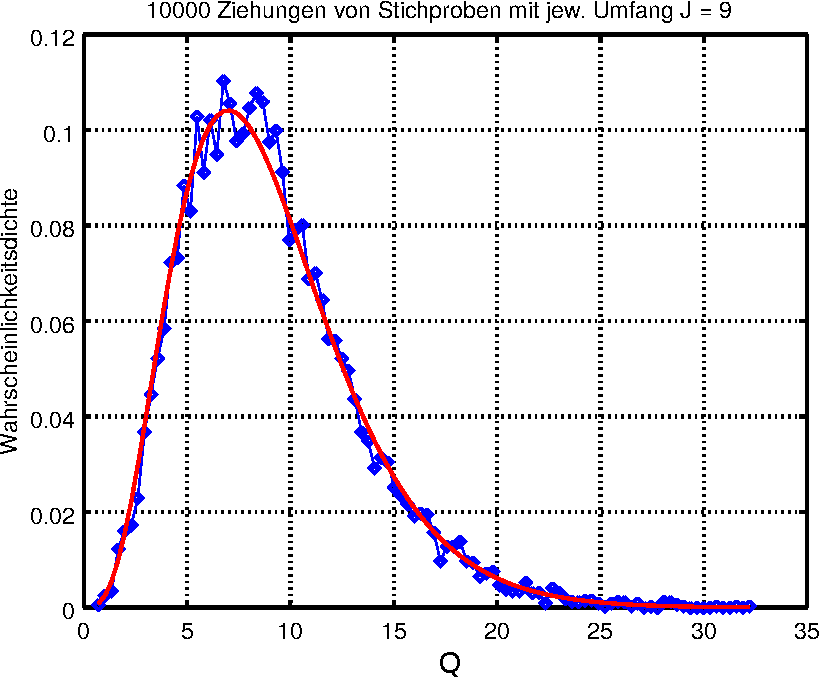
\includegraphics[width=75mm]{05_vorlesung/media/understandchi2_df9_final.pdf} \hspace{5mm}
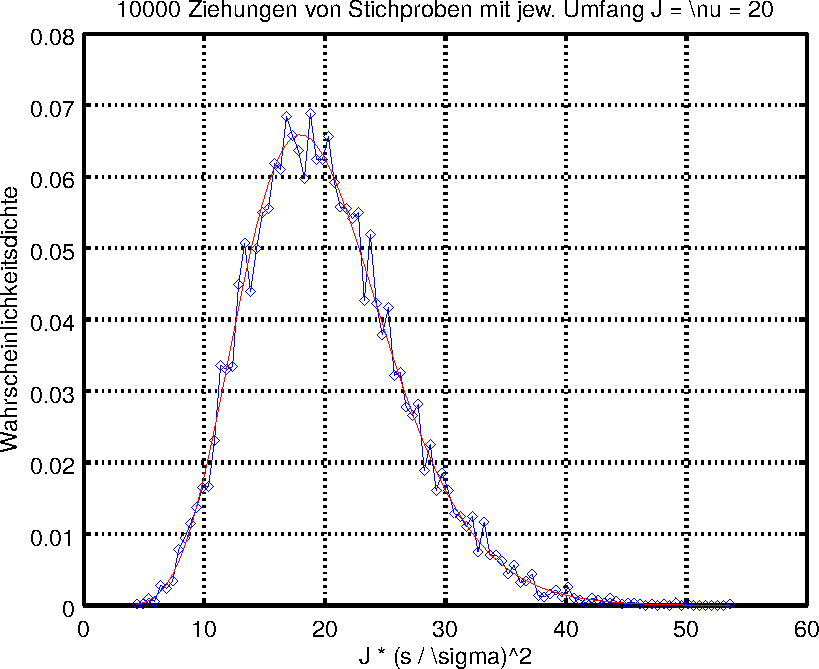
\includegraphics[width=75mm]{05_vorlesung/media/understandchi2_df20_final.pdf}
\caption{\label{ch2beispiele}$\chi^2$-Verteilung der normierten
Zufallsgröße $Q \; = \; J \, \left( \frac{s_{\mu}}{\sigma} \right)^2$ für
$s_{\mu}^2 \; = \; \frac{1}{J} \, \sum_{j=1}^{J} \, (X_{..,j} \, - \, \mu)^2$
für $J = 9$  (\textsl{links}) und $J = 20$ (\textsl{rechts}).}
\end{center}
\end{figure}

Abb.~\ref{ch2beispiele} zeigt zwei Beispiele für die Verteilungsdichte der Varianzen, zum einen
für $J = 9$ und zum anderen für $J = 20$. Mit
\begin{verbatim}
function understandchi2()
  Jz = 9;
  nbin = 100;
  n = 10000;
  d = zeros(n,1);
  for k=1:n
    x = randn(Jz,1);
    d(k) = sum(x.^2);
  end
  [haeuf, bin] = hist(d,nbin);
  Deltabin = bin(2)-bin(1);
  figure(1000);
  plot(bin,haeuf/(n*Deltabin),'bd-',bin,chi2pdf(bin,Jz),'r-');
  xlabel('J * (s / \sigma)^2', 'fontsize', 14);
  ylabel('Wahrscheinlichkeitsdichte', 'fontsize', 14);
  title([num2str(n) 'Stichprobenumfang J = \nu = ' num2str(Jz)], 'fontsize', 14);
  grid on;
  set(gca, 'fontsize', 14, 'linewidth', 2);
  print(1000,['understandchi2_df' num2str(Jz) '_solid.svg'],'-dsvg');
\end{verbatim}
wurden die Diagramme erzeugt. Die Verteilung der Grundgesamtheit ist die
Standardnormalverteilung mit $\mu = 0$ und $\sigma = 1$.
Eine Stichprobenentnahme wird mit \texttt{x = randn(Jz,1);} simuliert.

Wie bei der Quantildefinition für die Standardnormalverteilung und für die $t$-Verteilung
ist das Quantil der $\chi^2$-Verteilung die obere Integrationsgrenze
zur Gewinnung des Flächeninhalts der Verteilungsdichte. Dies quantifiziert die Wahrscheinlichkeit,
mit der für die Größe $Q$ Werte beobachtet werden, die kleiner sind als das Quantil.
Hier ist die untere Integrationsgrenze Null und nicht minus Unendlich, weil $Q$ per
Definitionem nur positive Werte haben kann, siehe Abb.~\ref{chi2quantil}.
\begin{figure}
\begin{center}
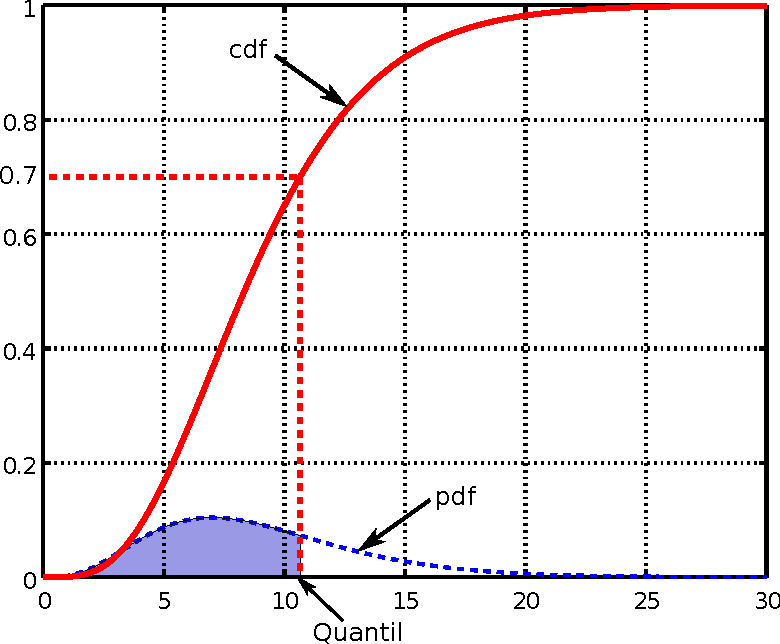
\includegraphics[width=100mm]{05_vorlesung/media/chiquadrat.pdf}
\caption{\label{chi2quantil}Wahrscheinlichkeitsverteilungsdichte (pdf) und
kumulierte Wahrscheinlichkeitsfunktion (cdf)
der normierten Varianzen, das Quantil wird $\chi^2$ genannt. Hier für 
$\nu = 9$ Freiheitgrade und $1 - \alpha = 0.7$, somit $\chi^2_{\nu, 1-\alpha} = 10.66$
dargestellt.}
\end{center}
\end{figure}
\begin{equation}
P(Q) \; = \; 
\int \limits_0^{\chi^2_{1-\alpha, \nu}}
p(Q^\prime, \nu) \; \operatorname{d} Q^\prime \; = \;
1 \, - \, \alpha
\label{chiQuadratQuantil}
\end{equation}
Für den $\chi^2$-Test wird, weil der Erwartungswert der Grundgesamtheit nicht bekannt ist,
die Varianz durch die empirische Varianz 
\begin{equation}
s_{\mu,i}^2 \; = \; \frac{1}{J_i} \, \sum_{j=1}^{J_i} \, (X_{i,j} \, - \, \mu)^2
\; \approx \; \frac{1}{J_i-1} \, \sum_{j=1}^{J_i} \, (X_{i,j} \, - \, y_i)^2
\; = \; s_i^2
\end{equation}
approximiert.
\begin{verbatim}
  for k=1:n
    x = randn(Jz,1);
    y = mean(x);
    d(k) = sum((x-y).^2);
  end
\end{verbatim}
Dann ist die Anzahl der Freiheitsgrade $\nu = J-1$ um einen vermindert,
weil der Mittelwert $y_i$ von den Werten $X_{i,j}$ abhängt. Die $\chi^2$-Verteilung
ist mit der Anzahl der Freiheitsgrade und nicht mit dem Stichprobenumfang zu verwenden
\begin{equation}
s^2 \; = \; \frac{1}{\nu} Q \, \sigma^2  \qquad \Leftrightarrow \qquad 
Q \; = \; \nu \, \left( \frac{s}{\sigma} \right)^2 ,
\label{s2Qempir}
\end{equation}
so dass die $\chi^2$-Verteilungsdichte, hier mit dem Funktionsaufruf
\texttt{chi2pdf} für $\nu = J-1$ zu verwenden ist:
\begin{verbatim}
  [haeuf, bin] = hist(d,nbin);
  Deltabin = bin(2)-bin(1);
  plot(bin,haeuf/(n*Deltabin),'bd-',bin,chi2pdf(bin,Jz-1),'r-');
  xlabel('(J-1) * (s / \sigma)^2', 'fontsize', 14);
\end{verbatim}

Für den Fall, den wir weiter oben betrachtet hatten, nämlich dass für den Erwartungswert
$\mu$ nicht sein Schätzer (der Mittelwert) verwendet wird, ist die Anzahl der
Freiheitsgrade gleich dem Stichprobenumfang.

Beim Chi-Quadrat-Test wird geprüft, ob die Varianz einer Stichprobe gleich einer
spezifizierten Varianz $\sigma_0^2$ ist. Wir formulieren die Hypothesen
\begin{center}
\begin{tabular}{c|cl}
$H_0$ & $\sigma^2 = \sigma_0^2$ & die Stichprobe gehört zu einer Grundgesamtheit mit der Varianz $\sigma_0^2$\\
\hline
$H_\mathrm{a}$ & $\sigma^2 \neq \sigma_0^2$ & die Stichprobe gehört nicht zu einer Grundgesamtheit mit der Varianz $\sigma_0^2$
\end{tabular}
\end{center}
Die Testgröße ist
\begin{equation}
T \; = \; \nu \, \left( \frac{s}{\sigma_0} \right)^2
\end{equation}
Die Nullhypothese wird mit einem Signifikanzniveau von $\alpha$
verworfen, falls die Testgröße außerhalb des Intervalls liegt,
das durch die in Gl.~(\ref{chiQuadratQuantil}) definierten Quantile begrenzt wird, d.h.
\begin{equation}
T \; < \; \chi^2_{\alpha, \nu}  \qquad \mathrm{oder} \qquad
T \; > \; \chi^2_{1-\alpha, \nu} .
\end{equation}

\begin{verbatim}
http://www.itl.nist.gov/div898/handbook/eda/section3/eda358.htm
\end{verbatim} 

\section{Anwendung von Hypothesentests}

Anwendung finden die Hypothesentests im Bereich der Qualitätssicherung in der Produktion (siehe beispielsweise
zur Prüfung des Stout in der Guinessbrauerei schon vor 100 Jahren), oder im Bereich der Naturwissenschaften
(Biologie, Chemie, Pharmazie, Medizien) zum Nachweis von Substanzen. Es geht darum, dass zu bewerten ist,
mit welcher Wahrscheinlichkeit Beobachtungen zu welcher Verteilung gehören.
Einer Entscheidung liegen Regeln zugrunde. Mit dem t-Test haben wir die Regeln kennengelernt, über
die wir entscheiden, ob zwei Datensätze zu der gleichen gaußverteilten Grundgesamtheit - der gleichen
Normalverteilung mit demselben Erwartungswert gehören. 

Als nächstes wollen wir untersuchen, welche Fehler mit welcher Wahrscheinlichkeit dabei entstehen können.
Anschließend wollen wir uns ansehen, wie eine Stichprobe mit einer Toleranzvorgabe verglichen wird.
Die Toleranzvorgabe liefert ein Intervall, dessen Lage mit der Lage der Wahrscheinlichkeitsverteilung
der zu untersuchenden Stichprobe verglichen wird.

\subsection{Entscheidung bei Vergleich zweier Stichproben}
\begin{figure}
\begin{center}
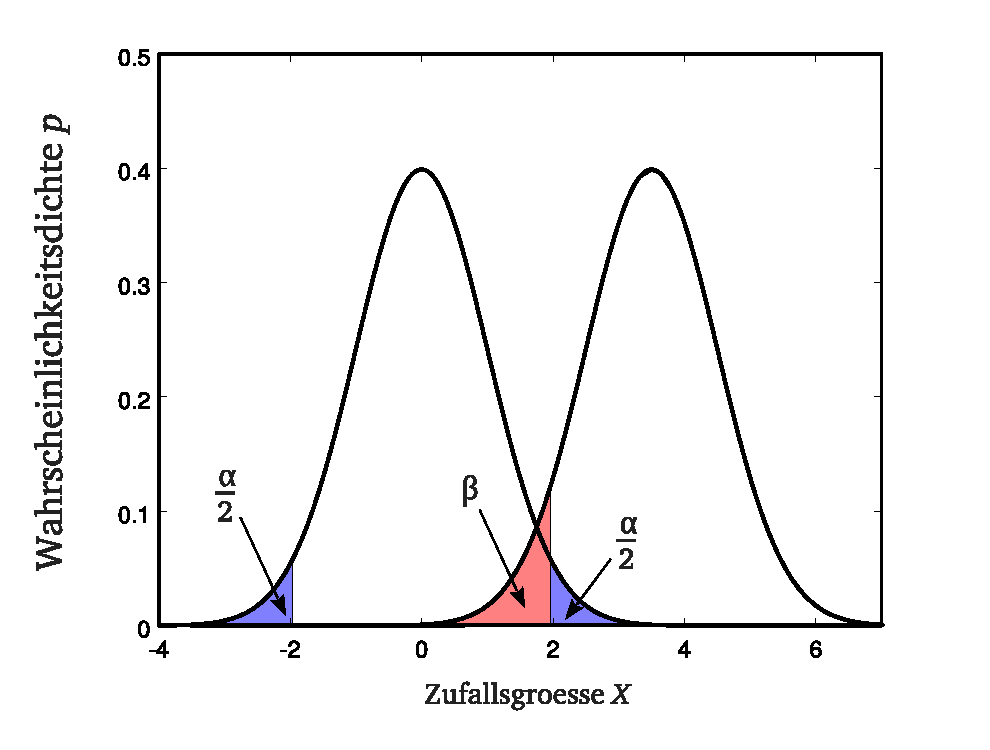
\includegraphics[width=100mm]{05_vorlesung/media/entscheidungsfehlertypen.pdf}
\caption{\label{entscheidungsfehler} Die Ereignisse (beobachtete Werte) aus der linken Wahrscheinlichkeitsdichteverteilung,
 die in deren \textsl{Tails} liegen, werden mit einem Signifikanzniveau von $\alpha$ verworfen.
 Die Ereignisse (beobachtete Werte) aus der rechten Wahrscheinlichkeitsdichteverteilung, die in dessen linkem
 \textsl{Tail} liegen, werden mit Wahrscheinlichkeit $\beta$ als der linken Wahrscheinlichkeit zugehörig
 erachtet.}
\end{center}
\end{figure}
Den Hypothesentests, die wir uns angesehen haben, ist gemeinsam, dass
\begin{enumerate}
\item eine Nullhypothese $H_0$ (evtl.\ auch eine Alternativhypothese $H_\mathrm{a}$)
aufgestellt wurde,
\item ein Signifikanzniveau $\alpha$ spezifiziert wurde,
\item eine Stichprobe mit einer Anzahl Freiheitsgrade $\nu$
genommen wurde und
\item anhand der vorher aufgestellten Entscheidungsregeln (Vergleich einer
Prüfgröße mit dem Quantil einer Wahrscheinlichkeitsdichteverteilung)
die Hypothese verworfen oder angenommen wurde.
\end{enumerate}
In der Entscheidungsregel werden durch Vorgabe eines Signifikanzniveaus Verwerfungsbereich
und Annahmebereich festgelegt. Das Signifikanzniveau ist dabei Komplementärwahrscheinlichkeit
(Gegenwahrscheinlichkeit) zum Vertrauensniveau, das ist die Wahrscheinlichkeit dafür
wie sicher die Hypothese ist.

Die Wahrscheinlichkeit, mit einem Hypothesentest eine falsche
Entscheidung zu treffen wird in zwei Klassen von Fehlern aufgeteilt, den
$\alpha$-Fehler oder den $\beta$-Fehler

\begin{center}
\begin{tabular}{M{3cm}|M{5.5cm}|M{5.5cm} N}
                 &     $H_0$ annehmen    &     $H_0$ ablehnen   \\[3pt]
\hline
$H_0$ ist wahr   & richtige Entscheidung, Wahrscheinlichkeit: $1-\alpha$ & Fehler 1.\ Art, Wahrscheinlichkeit $\alpha$ \\[3pt]
\hline
$H_0$ ist falsch & Fehler 2.\ Art, Wahrscheinlichkeit: $\beta$  & richtige Entscheidung, Wahrscheinlichkeit: $1-\beta$
\end{tabular}
\end{center}

Abb.~\ref{entscheidungsfehler} soll illustrieren, dass Beobachtungswerte, die zu einer
Grundgesamtheit mit einer Wahrscheinlichkeitsdichteverteilung mit Erwartungswert
$\mu_\mathrm{a} = 3.5$ gehören, per Hypothesentest einer Grundgesamtheit mit $\mu_0 = 0$
zugeordnet werden. Die Wahrscheinlichkeit für das Auftreten solcher Beobachtungen ist
dann $\beta$. Das Diagramm wurde mit folgendem Octaveskript erzeugt

\begin{verbatim}
function plot_entscheidungsfehler()
  dz = 0.02;
  lim = 7;
  z = [-lim:dz:lim];
  p1 = normpdf(z,0,1);
  t = 1.96;
  zleft = [-lim:dz:-t];
  pleft = normpdf(zleft,0,1);
  zright = [t:dz:lim];
  pright = normpdf(zright,0,1);
  mu2 = 3.5;
  p2 = normpdf(z+mu2,mu2,1);
  zbeta = [mu2-lim:dz:t];
  pbeta = normpdf(zbeta,mu2,1);
  figure(200); hold on;
  area( zleft, pleft, 'Facecolor', [0.5 0.5 1]);
  area( zright, pright, 'Facecolor', [0.5 0.5 1]);
  area( zbeta, pbeta, 'Facecolor', [1 0.5 0.5]);
  plot( z, p1, 'k-', 'linewidth', 2);
  plot( z+mu2, p2, 'k--', 'linewidth', 2);
  xlabel('X', 'fontsize', 14);
  ylabel('p', 'fontsize', 14);
  axis([-4 7 0 0.5]);
  set(gca, 'fontsize', 14);
  hold off;
  print(200, 'entscheidungsfehler.svg', '-dsvg');
end
\end{verbatim}

\subsection{Konformitätswahrscheinlichkeiten}
Nachdem wir gesehen haben wie wir zwei Hypothesen über die Lage zweier Wahrscheinlichkeitsdichteverteilungen
verglichen haben, befassen wir uns jetzt mit dem Vergleich eines Intervalls, einem Toleranzintervall, mit einer
Wahrscheinlichkeitsdichteverteilung. Für die Fertigung werden in den Konstruktionszeichnungen zu den Merkmalen
von Bauteilen die Toleranzen eingetragen, innerhalb derer die Merkmale des Werkstücks liegen müssen. Wie nun
bewertet man nach Fertigstellung des Werkstücks, ob ein Merkmal innerhalb einer Toleranzvorgabe liegt? Ein Merkmal
wird durch einen Messvorgang geprüft. Der Messvorgang liefert ein Ergebnis: Einen Zahlenwert für das Merkmal und
ein Überdeckungsintervall zusammen mit einem Vertrauensniveau. Anstelle von Überdeckungsintervall und Vertrauensniveau
kann auch direkt eine Wahrscheinlichkeitsdichteverteilung angegeben werden, ist aber sehr unüblich in der industriellen
Praxis. Für die Bewertung, ob das gefertigte Werkstück mit der Vorgabe der Konstruktion übereinstimmt, konform ist,
werden Messergebnis und Toleranzvorgabe verglichen.

Als Ergänzung zum \glqq Guide of Uncertainty\grqq gibt es das Dokument
\textsl{Evaluation of measurement data - The role of measurement uncertainty in conformity assessment},
das darlegt, wie Konformitätsbewertungen vorzunehem sind.
\begin{verbatim}
https://www.bipm.org/utils/common/documents/jcgm/JCGM_106_2012_E.pdf
\end{verbatim}
Dort heißt es in Paragraph 7.1.1
\begin{quote}
An item conforms to a specified requirement if the true value of its associated property $Y$ lies in the tolerance
interval. Knowledge of $Y$ is conveyed by a probability density function $p(y|{X_1,\dots,X_J})$
so that a statement of conformity is always an inference,
with some probability of being true. Denoting the set of permissible (conforming) values
$Y$ by $C$, the conformance probability, denoted by $p_\mathrm{c}$, is given by
\begin{equation}
	p_\mathrm{c} = P(Y \in C | {X_1,\dots,X_J}) = \int\limits_C p(y|{X_1,\dots,X_J}) \mathrm{d}y.
\end{equation}
\end{quote}
Im Originaldokument werden Sie eine etwas andere Schreibweise für die Bezeichner in der Formel vorfinden.
Hier ist es so aufgeschrieben, wie es zu der Notation innerhalb dieses Vorlesungsskriptes, insbesondere
zu Kapitel \ref{KonzepteinverseProbleme}, passt.
Für die Toleranz wird in der Richtlinie zur Konformitätsbewertung zur Wahrung der Allgemeingültigkeit
eine Menge $C$ angegeben. Falls die Größe $Y$ eine skalarwertige Größe wie bei dem Beispiel, anhand dessen
wir in Kapitel \ref{KonzepteinverseProbleme} das Prinzip der bayesischen Statistik illustriert haben,
so steht $C$ für ein Intervall $C = [y_\mathrm{L}, y_\mathrm{U}]$. Dabei sollen der Index L für \glqq lower
limit\grqq ~und der Index U für \glqq upper limit\grqq ~stehen.

Die Wahrscheinlichkeit $p_\mathrm{c}$, dass die Beobachtungen ${X_1,\dots,X_J}$ innerhalb des Toleranzintervalls
$C = [y_\mathrm{L}, y_\mathrm{U}]$ liegen, ist
\begin{equation}
	p_\mathrm{c} =  \int\limits_{y_\mathrm{L}}^{y_\mathrm{U}} p(y|{X_1,\dots,X_J}) \mathrm{d}y.
\end{equation}
Für den Fall, dass von einer normalverteilten Stichprobe ausgegangen werden kann und dass eine Einzelgröße
vorliegt, wird auch der Stichprobe ${X_1,\dots,X_J}$ der Schätzer $\bar y$ aus einfacher Mittelwertbildung
gewonnen ($\bar y = \sum_{j=1}^J X_j$) und die Varianz als empirische Varianz $s$ aus
$s = \frac{1}{J-1}\sum (X_j - \bar y)^2$ und für die Wahrscheinlichkeitsdichte $p$ die Gaußverteilung:
\begin{equation}
	p_\mathrm{c} = \frac{1}{\sqrt{2 \pi} s} \int\limits_{y_\mathrm{L}}^{y_\mathrm{U}} 
	e^{-\frac{1}{2}\left(\frac{y - \bar y}{s}\right)^2} \mathrm{d}y
\end{equation}
Die Größe $\frac{y - \bar y}{s}$ ist eine normierte Zufallsgröße. Die Integrationsgrenzen können gleichfalls
normiert werden: $z = \frac{y - \bar y}{s}$, $z_\mathrm{L} = \frac{y_\mathrm{L} - \bar y}{s}$ und
$z_\mathrm{U} = \frac{y_\mathrm{U} - \bar y}{s}$, so dass die Tabellenwerke oder Bibliotheksfunktion
für die gauß'sche Fehlerfunktion (\textsl{error function}) wie folgt verwendet werden kann:
\begin{equation}
p_\mathrm{c} = \frac{1}{\sqrt{2 \pi}} \int\limits_{-\infty}^{z_\mathrm{U}} 
	e^{-\frac{1}{2} z^2} \mathrm{d}z - 
	\frac{1}{\sqrt{2 \pi}} \int\limits_{-\infty}^{z_\mathrm{L}} e^{-\frac{1}{2} z^2} \mathrm{d}z
\end{equation}
d.h.
\begin{equation}
	p_\mathrm{c} = \mathrm{erf}(z_\mathrm{U}) - \mathrm{erf}(z_\mathrm{L}).
\end{equation}


%\bibliography{$BIBLIO/math}
%\bibliographystyle{unsrt}


\section{Übungsaufgaben zum Selbststudium}
\label{AufgVorl5}

\textbf{Aufgabe 1}\\

Probieren Sie anhand von Beobachtungen, die Sie mit Hilfe eines Generators, der
normalverteilte Zufallszahlen liefert, den Kolmogorow-Smirnow-Test, kurz KS-Test, aus.

In Matlab/Gnu-Octave könnten Sie dies beispielsweise wie folgt realisieren:
\begin{verbatim}
  J1 = 2000; % Stichprobenumfang
  mu1 = 23; % Erwartungswert der Zufallsgroesse
  s1 = 3;   % Wurzel aus dem Erwartungswert fuer die Varianz
  Xarray = s1*randn(J1,1) + mu1;
\end{verbatim}
Das Sortieren mit Matlab/Gnu-Octave können Sie mit
\begin{verbatim}
  [xsort, isort] = sort(Xarray, 'ascend');
\end{verbatim}
und die Wahrscheinlichkeiten mit
\begin{verbatim}
  h = [1:J1]'/J1;
\end{verbatim}
berechnen.

\begin{enumerate}
\item Verwenden Sie nicht die {\`a} priori eingesetzten Erwartungswerte,
 sondern Mittelwert \texttt{y = mean(Xarray)} und empirische Standardabweichung
 \texttt{s = std(Xarray)}, um die Funktion $P(X)$ aus Gl.~(\ref{cdfKS})
 zu realisieren. Berechnen Sie die relativen Häufigkeiten $H$ gemäß
 Gl.~(\ref{cdfH}), sowie den in Gl.~(\ref{KSpruefgroesse}) definierten
 Schwellwert
  $$K_{\alpha, J}$$
 zu einem Signifikanzniveau von $\alpha = 0.05$,
 wobei $J$ der Stichprobenumfang ist.
 Führen Sie den Test mit den von Ihnen erzeugten Zufallswerten durch.
\item Erzeugen Sie einen zusätzlichen Satz von Zufallszahlen, beispielsweise mit den
 Werten \texttt{mu2 = 35} und \texttt{s2 = 5}. Wählen Sie für diese einen
 deutlich kleineren Stichprobenumfang. Führen Sie den KS-Test für die
 vereinigten Zufallszahlenarrays durch und tun Sie so, als ob Sie nicht
 wüssten, dass dies keine gemeinsame Grundgesamtheit ist.
\end{enumerate}



\textbf{Aufgabe 2}

Gegeben seien zwei Stichproben

Stichprobe 1:

\begin{tabular}{|c|c|c|c|c|}
\hline
21 & 33 & 19 & 39 & 7\\
\hline
\end{tabular}

Stichprobe 2:

\begin{tabular}{|c|c|c|c|c|c|c|c|c|}
\hline
53 & 69 & 63 & 47 & 49 & 44 & 47 & 44 & 38\\
\hline
\end{tabular}

\begin{enumerate}
\item[a)] Geben Sie zu jeder der beiden Stichproben die Mittelwerte und Standardabweichungen an.
\item[b)] Prüfen Sie auf einem Signifikanzniveau von $\alpha = 0.05$ die Hypothese $H_0$,
 ob beide Stichproben zu einer Grundgesamtheit
 mit demselben Erwartungswert $\mu$ gehören. Geben Sie dazu die Formel und den Wert
 der Testgröße an und vergleichen Sie diese mit dem entsprechenden Quantil der für diesen
 Test zu verwendenden Verteilung. Mit welcher Verteilung ist dieser Test durchzuführen?
\item[c)] Prüfen Sie auf einem Signifikanzniveau von $\alpha = 0.05$ die Hypothese $H_0$,
 ob die zweite Stichprobe zu einer Grundgesamtheit
 mit der Standardabweichung $\sigma_0 = 6$ gehört. Geben Sie dazu die Formel und den Wert
 der Testgröße an und vergleichen Sie diese mit dem entsprechenden Quantil der für diesen
 Test zu verwendenden Verteilung. Mit welcher Verteilung ist dieser Test durchzuführen?
 Führen Sie nur den einseitigen Test durch, das heißt prüfen Sie nur bezüglich
 des rechten \textsl{Tail} der Verteilungsdichte.
\item[d)] Führen Sie denselben Test wie in (c) durch, aber dieses Mal für $\sigma_0 = 9$.
\end{enumerate}

Verwenden Sie die auf den folgenden Seiten abgedruckten Quantiltabellen.

\pagebreak

\section{Quantiltabellen}

\subsection{Quantile der Student-t Verteilung}
\begin{tabular}{c||c|c|c|c|c|}
d.o.f & \multicolumn{5}{c|}{Wahrscheinlichkeit}\\
\hline
$\nu$ & 0.995 & 0.990 & 0.975 & 0.950 & 0.800 \\ 
\hline\hline
2 & 9.925 & 6.965 & 4.303 & 2.920 & 1.061 \\ 
\hline
3 & 5.841 & 4.541 & 3.182 & 2.353 & 0.978 \\ 
\hline
4 & 4.604 & 3.747 & 2.776 & 2.132 & 0.941 \\ 
\hline
5 & 4.032 & 3.365 & 2.571 & 2.015 & 0.920 \\ 
\hline
6 & 3.707 & 3.143 & 2.447 & 1.943 & 0.906 \\ 
\hline
7 & 3.499 & 2.998 & 2.365 & 1.895 & 0.896 \\ 
\hline
8 & 3.355 & 2.896 & 2.306 & 1.860 & 0.889 \\ 
\hline
9 & 3.250 & 2.821 & 2.262 & 1.833 & 0.883 \\ 
\hline
10 & 3.169 & 2.764 & 2.228 & 1.812 & 0.879 \\ 
\hline
11 & 3.106 & 2.718 & 2.201 & 1.796 & 0.876 \\ 
\hline
12 & 3.055 & 2.681 & 2.179 & 1.782 & 0.873 \\ 
\hline
13 & 3.012 & 2.650 & 2.160 & 1.771 & 0.870 \\ 
\hline
14 & 2.977 & 2.624 & 2.145 & 1.761 & 0.868 \\ 
\hline
15 & 2.947 & 2.602 & 2.131 & 1.753 & 0.866 \\ 
\hline
16 & 2.921 & 2.583 & 2.120 & 1.746 & 0.865 \\ 
\hline
17 & 2.898 & 2.567 & 2.110 & 1.740 & 0.863 \\ 
\hline
18 & 2.878 & 2.552 & 2.101 & 1.734 & 0.862 \\ 
\hline
19 & 2.861 & 2.539 & 2.093 & 1.729 & 0.861 \\ 
\hline
20 & 2.845 & 2.528 & 2.086 & 1.725 & 0.860 \\ 
\hline
21 & 2.831 & 2.518 & 2.080 & 1.721 & 0.859 \\ 
\hline
22 & 2.819 & 2.508 & 2.074 & 1.717 & 0.858 \\ 
\hline
23 & 2.807 & 2.500 & 2.069 & 1.714 & 0.858 \\ 
\hline
24 & 2.797 & 2.492 & 2.064 & 1.711 & 0.857 \\ 
\hline
25 & 2.787 & 2.485 & 2.060 & 1.708 & 0.856 \\ 
\hline
\end{tabular}
\hspace{7mm}
\begin{tabular}{c||c|c|c|c|c|}
d.o.f & \multicolumn{5}{c|}{Wahrscheinlichkeit}\\
\hline
$\nu$ & 0.995 & 0.990 & 0.975 & 0.950 & 0.800 \\ 
\hline\hline
26 & 2.779 & 2.479 & 2.056 & 1.706 & 0.856 \\ 
\hline
27 & 2.771 & 2.473 & 2.052 & 1.703 & 0.855 \\ 
\hline
28 & 2.763 & 2.467 & 2.048 & 1.701 & 0.855 \\ 
\hline
29 & 2.756 & 2.462 & 2.045 & 1.699 & 0.854 \\ 
\hline
30 & 2.750 & 2.457 & 2.042 & 1.697 & 0.854 \\ 
\hline
31 & 2.744 & 2.453 & 2.040 & 1.696 & 0.853 \\ 
\hline
32 & 2.738 & 2.449 & 2.037 & 1.694 & 0.853 \\ 
\hline
33 & 2.733 & 2.445 & 2.035 & 1.692 & 0.853 \\ 
\hline
34 & 2.728 & 2.441 & 2.032 & 1.691 & 0.852 \\ 
\hline
35 & 2.724 & 2.438 & 2.030 & 1.690 & 0.852 \\ 
\hline
36 & 2.719 & 2.434 & 2.028 & 1.688 & 0.852 \\ 
\hline
37 & 2.715 & 2.431 & 2.026 & 1.687 & 0.851 \\ 
\hline
38 & 2.712 & 2.429 & 2.024 & 1.686 & 0.851 \\ 
\hline
39 & 2.708 & 2.426 & 2.023 & 1.685 & 0.851 \\ 
\hline
40 & 2.704 & 2.423 & 2.021 & 1.684 & 0.851 \\ 
\hline
41 & 2.701 & 2.421 & 2.020 & 1.683 & 0.850 \\ 
\hline
42 & 2.698 & 2.418 & 2.018 & 1.682 & 0.850 \\ 
\hline
43 & 2.695 & 2.416 & 2.017 & 1.681 & 0.850 \\ 
\hline
44 & 2.692 & 2.414 & 2.015 & 1.680 & 0.850 \\ 
\hline
45 & 2.690 & 2.412 & 2.014 & 1.679 & 0.850 \\ 
\hline
46 & 2.687 & 2.410 & 2.013 & 1.679 & 0.850 \\ 
\hline
47 & 2.685 & 2.408 & 2.012 & 1.678 & 0.849 \\ 
\hline
48 & 2.682 & 2.407 & 2.011 & 1.677 & 0.849 \\ 
\hline
49 & 2.680 & 2.405 & 2.010 & 1.677 & 0.849 \\ 
\hline
50 & 2.678 & 2.403 & 2.009 & 1.676 & 0.849 \\ 
\hline
\end{tabular}


\subsection{Quantile der $\chi^2$-Verteilung}

\begin{small}
\begin{tabular}{c||c|c|c|c|c|}
 & \multicolumn{5}{c|}{Wahrscheinlichkeit}\\
\hline
$\nu$ & 0.995 & 0.990 & 0.975 & 0.950 & 0.800 \\ 
\hline\hline
2 & 10.597 & 9.210 & 7.378 & 5.991 & 3.219 \\ 
\hline
3 & 12.838 & 11.345 & 9.348 & 7.815 & 4.642 \\ 
\hline
4 & 14.860 & 13.277 & 11.143 & 9.488 & 5.989 \\ 
\hline
5 & 16.750 & 15.086 & 12.833 & 11.070 & 7.289 \\ 
\hline
6 & 18.548 & 16.812 & 14.449 & 12.592 & 8.558 \\ 
\hline
7 & 20.278 & 18.475 & 16.013 & 14.067 & 9.803 \\ 
\hline
8 & 21.955 & 20.090 & 17.535 & 15.507 & 11.030 \\ 
\hline
9 & 23.589 & 21.666 & 19.023 & 16.919 & 12.242 \\ 
\hline
10 & 25.188 & 23.209 & 20.483 & 18.307 & 13.442 \\ 
\hline
11 & 26.757 & 24.725 & 21.920 & 19.675 & 14.631 \\ 
\hline
12 & 28.300 & 26.217 & 23.337 & 21.026 & 15.812 \\ 
\hline
13 & 29.819 & 27.688 & 24.736 & 22.362 & 16.985 \\ 
\hline
14 & 31.319 & 29.141 & 26.119 & 23.685 & 18.151 \\ 
\hline
15 & 32.801 & 30.578 & 27.488 & 24.996 & 19.311 \\ 
\hline
16 & 34.267 & 32.000 & 28.845 & 26.296 & 20.465 \\ 
\hline
17 & 35.718 & 33.409 & 30.191 & 27.587 & 21.615 \\ 
\hline
18 & 37.156 & 34.805 & 31.526 & 28.869 & 22.760 \\ 
\hline
19 & 38.582 & 36.191 & 32.852 & 30.144 & 23.900 \\ 
\hline
20 & 39.997 & 37.566 & 34.170 & 31.410 & 25.038 \\ 
\hline
21 & 41.401 & 38.932 & 35.479 & 32.671 & 26.171 \\ 
\hline
22 & 42.796 & 40.289 & 36.781 & 33.924 & 27.301 \\ 
\hline
23 & 44.181 & 41.638 & 38.076 & 35.172 & 28.429 \\ 
\hline
24 & 45.559 & 42.980 & 39.364 & 36.415 & 29.553 \\ 
\hline
25 & 46.928 & 44.314 & 40.646 & 37.652 & 30.675 \\ 
\hline
\end{tabular}
\hspace{2mm}
\begin{tabular}{c||c|c|c|c|c|}
 & \multicolumn{5}{c|}{Wahrscheinlichkeit}\\
\hline
$\nu$ & 0.995 & 0.990 & 0.975 & 0.950 & 0.800 \\ 
\hline\hline
26 & 48.290 & 45.642 & 41.923 & 38.885 & 31.795 \\ 
\hline
27 & 49.645 & 46.963 & 43.195 & 40.113 & 32.912 \\ 
\hline
28 & 50.993 & 48.278 & 44.461 & 41.337 & 34.027 \\ 
\hline
29 & 52.336 & 49.588 & 45.722 & 42.557 & 35.139 \\ 
\hline
30 & 53.672 & 50.892 & 46.979 & 43.773 & 36.250 \\ 
\hline
31 & 55.003 & 52.191 & 48.232 & 44.985 & 37.359 \\ 
\hline
32 & 56.328 & 53.486 & 49.480 & 46.194 & 38.466 \\ 
\hline
33 & 57.648 & 54.776 & 50.725 & 47.400 & 39.572 \\ 
\hline
34 & 58.964 & 56.061 & 51.966 & 48.602 & 40.676 \\ 
\hline
35 & 60.275 & 57.342 & 53.203 & 49.802 & 41.778 \\ 
\hline
36 & 61.581 & 58.619 & 54.437 & 50.998 & 42.879 \\ 
\hline
37 & 62.883 & 59.893 & 55.668 & 52.192 & 43.978 \\ 
\hline
38 & 64.181 & 61.162 & 56.896 & 53.384 & 45.076 \\ 
\hline
39 & 65.476 & 62.428 & 58.120 & 54.572 & 46.173 \\ 
\hline
40 & 66.766 & 63.691 & 59.342 & 55.758 & 47.269 \\ 
\hline
41 & 68.053 & 64.950 & 60.561 & 56.942 & 48.363 \\ 
\hline
42 & 69.336 & 66.206 & 61.777 & 58.124 & 49.456 \\ 
\hline
43 & 70.616 & 67.459 & 62.990 & 59.304 & 50.548 \\ 
\hline
44 & 71.893 & 68.710 & 64.201 & 60.481 & 51.639 \\ 
\hline
45 & 73.166 & 69.957 & 65.410 & 61.656 & 52.729 \\ 
\hline
46 & 74.437 & 71.201 & 66.617 & 62.830 & 53.818 \\ 
\hline
47 & 75.704 & 72.443 & 67.821 & 64.001 & 54.906 \\ 
\hline
48 & 76.969 & 73.683 & 69.023 & 65.171 & 55.993 \\ 
\hline
49 & 78.231 & 74.919 & 70.222 & 66.339 & 57.079 \\ 
\hline
50 & 79.490 & 76.154 & 71.420 & 67.505 & 58.164 \\ 
\hline
\end{tabular}
\end{small}




%
\chapter{Auswertung von Mess- und Ringvergleichen}
%\include{06_vorlesung/06_Ringvergleiche}
%
\chapter{Messunsicherheitsfortpflanzung bei linearen Modelle}
\label{unsicherheitsfortpfLin}
%\include{07_vorlesung/07_Unsicherheitsfortpf_lin}
%
\chapter{Auswertung von Mess- und Ringvergleichen}
%
\chapter{Messunsicherheitsfortpflanzung\\ linearer Modelle}
%
\chapter{Lösungen zu den Aufgaben\\ zum Selbststudium}
\section{Lösungen zu den Aufgaben aus Vorl 2}
\subsection{Lösung zur 1. Aufgabe: Lineare Regression}
siehe \ref{Vorl2Regressionsaufg1}

zu (a) Stellen Sie das lineare Gleichungssystem auf, das sich durch partielles Ableiten
für das Optimierungsproblem
$$
\min\limits_{a,c,h} \left\{\sum_{j=1}^{J_T} \varepsilon_j^2\right\}
$$
ergibt, mit $J_T = 21$.

Die Modellgleichung lautet
\begin{equation}
z_j \; = \; a \, x_j \, + \, c \, + \, h \, \delta_{j \in C} \; + \; \varepsilon_j
\label{Modellgl1}
\end{equation}
In Vektorschreibweise mit $\boldsymbol x$ und $\boldsymbol z$ als Spaltenvektoren sieht 
dies mit allen in der oben aufgeführten Werten wie folgt aus
$$
\boldsymbol x = \left(
\begin{array}{c}
0\\
0.25\\
0.50\\
\vdots\\
2.25\\
2.75\\
\vdots\\
5.00
\end{array}\right) \qquad
\boldsymbol x_1 = \left(
\begin{array}{c}
1\\
1\\
1\\
\vdots\\
1\\
0\\
\vdots\\
0
\end{array}\right)  \qquad
\boldsymbol x_0 = \left(
\begin{array}{c}
1\\
1\\
1\\
\vdots\\
1\\
1\\
\vdots\\
1
\end{array}\right) \qquad
\boldsymbol z = \left(
\begin{array}{c}
-54.08\\
-55.63\\
-44.65\\
\vdots\\
-60.77\\
36.85\\
\vdots\\
23.19
\end{array}\right)
$$
Für die Realisierung der Kroneckersymbols $\delta_{j \in C}$ wurde
der Spaltenvektor $\boldsymbol x_1$ definiert, der als erste
$J_C = 10$ Vektorkomponenten Einsen enthält und als weitere Vektorkomponenten Nullen.
Der Vektor $\boldsymbol x_0$ besteht nur aus Einsen.

Als nächstes ist es wichtig, die Größen auf dieselbe Dimension zu bringen,
so dass wir eine Steigung berechnen wollen, also rechnen wir die x-Werte auch in Mikrometern
$$
\boldsymbol x_2 \, = \, 1000 \, \boldsymbol x
$$
Somit sieht die Modellgleichung (\ref{Modellgl1}) wie folgt aus
$$
\boldsymbol z \; = \;  c \,  \boldsymbol x_0 \,  + \, h \, \boldsymbol x_1 \, + \, a \, \boldsymbol x_2 \, + \, \boldsymbol \varepsilon
$$
nun schreiben wir alle Spaltenvektoren mit x in eine gemeinsame Matrix, die dann 3 Spalten hat und $J_T = 21$ Zeilen
\begin{equation}
\boldsymbol X \; = \; \left(\boldsymbol x_0 \; \boldsymbol x_1 \; \boldsymbol x_2 \right)
\label{Regressormatrix}
\end{equation}
so dass die Modellgleichung wie folgt aussieht
$$
\boldsymbol \varepsilon  \; = \;  \boldsymbol z \, - \, \boldsymbol X
\left(\begin{array}{c}
c\\
h\\
a
\end{array}\right) .
$$
Wenn man diesen Ansatz in dieser Form hat, kann man einfach Gl.~(\ref{LsgRegressionGlSys}) 
verwenden und alles einsetzten.
Für die Klausur kommt es also nur darauf an, die Regressormatrix $\boldsymbol X$, das ist Gl.~(\ref{Regressormatrix})
aufstellen zu können und Gl.~(\ref{LsgRegressionGlSys}) aus dieser Vorlesung zu kennen:
\begin{equation}
\left( \mathbf{X}^\mathsf{T}  \, \mathbf{X} \right) \left(\begin{array}{c}
c\\
h\\
a
\end{array}\right) \; = \;
 \mathbf{X}^\mathsf{T} \, \mathbf{z} 
\end{equation}
wobei $\boldsymbol X^\mathsf{T}$ die transponierte Matrix ist, die in der ersten Zeile alles Einsen hat, in der
zweiten Zeile an den ersten $J_C = 10$ Spaltenpositionen Einsen und an den letzten 11 Nullen hat und in der dritten
und letzten Zeile die Werte $0.00 ~ 0.25 ~ 0.50 ~ 0.75 \dots ~5.00$ aus der Tabelle hat.
Hier ist dieser Teil der Aufgabenstellung fertig.


zu (b) Schreiben Sie die Gleichung für die Stufenhöhe $d$ als Funktion von $h$ und $a$ auf.
\begin{equation}
d \; = \; \frac{h}{\sqrt{1 + a^2}}
\end{equation}
Wer zuvor die x-Werte in Millimetern gerechnet hat, muss spätestens hier die Steigung
$a$ entsprechend umrechnen und durch $1000$ teilen.

zu (c) Schreiben Sie die Formel für die Varianz der Residuen auf.
$$
\sigma_\varepsilon^2 \; = \; \frac{1}{J_T - 3} \boldsymbol \varepsilon^\mathsf{T} \, \boldsymbol \varepsilon
$$

zu (d) Schreiben Sie die Formel für die Kovarianzmatrix der Modellparameter
$a, c, h$ auf.

Wir verwenden dazu Gl.~(\ref{UnsicherheitRegressparams}) dieser Vorlesung
\begin{equation}
\boldsymbol \Sigma \; = \; \left( \mathbf{X}^\mathsf{T}  \, \mathbf{X} \right)^{-1} \, \sigma_\varepsilon^2
\end{equation}
mit 

zu (e) Verwenden Sie eine Programmierumgebung Ihrer Wahl, Matlab, Octave, Python, R, ...
die Ihnen einen Solver für lineare Gleichungssysteme zur Verfügung stellt, sowie
eine Routine zur Matrixinversion und berechen Sie die Zahlenwerte für die Modellparameter
sowie deren Kovarianzmatrix.

\begin{verbatim}
function Lsg_Uebung_step()
%
% Teil (a)
  x = [0.00  0.25  0.50  0.75  1.00  1.25  1.50 ...
   1.75  2.00  2.25  2.50  2.75  3.00  3.25  3.50 ...
   3.75  4.00  4.25  4.50  4.75  5.00]';
  z = [-54.08 -55.63 -44.65 -51.44 -52.21 -58.01 ...
   -50.76 -56.01 -54.86 -60.77 36.85 38.02 31.71 36.21 ...
   23.39 29.01 30.11 29.35 20.81 33.27 23.19]';
  x2 = 1e3*x;
  J_T = 21;
  J_C = 10;
  x0 = ones(J_T,1);
  x1 = [ones(J_C,1);zeros(J_T-J_C,1)];
  X = [x0 x1 x2];
  XTX = X' * X;
  b = X' * z;
  theta = XTX \ b;
  printf('c = %1.4f um\n', theta(1));
  printf('h = %1.4f um\n', theta(2));
  printf('a = %1.7f um/um\n', theta(3));
\end{verbatim}
\begin{verbatim}
%
% Teil (b)
  d = theta(2) / sqrt(1 + theta(3)^2);
  printf('d = %1.4f um\n', d);
\end{verbatim}
\begin{verbatim}
%
% Teil (c)
  epsilon = z - X * theta;
  var_eps = (epsilon' * epsilon) / (J_T-3);
\end{verbatim}

~\\

\begin{verbatim}
%
% Teil (e)
  Kovarianz = inv(XTX) * var_eps;
  printf(' %e %e %e \n', Kovarianz(1,1), Kovarianz(1,2), Kovarianz(1,3));
  printf(' %e %e %e \n', Kovarianz(2,1), Kovarianz(2,2), Kovarianz(2,3));
  printf(' %e %e %e \n', Kovarianz(3,1), Kovarianz(3,2), Kovarianz(3,3));
\end{verbatim}

Ergebnisse:
\begin{verbatim}
c = 44.5660 um
h = -94.0905 um
a = -0.0038377 um/um
d = -94.0899 um
\end{verbatim}

$\Sigma =$
\begin{verbatim}
2.369818e+01 -1.710178e+01 -5.863466e-03
 -1.710178e+01 1.436549e+01 4.104426e-03
 -5.863466e-03 4.104426e-03 1.563591e-06
\end{verbatim}



\subsection{Lösung zur 2. Aufgabe: Lineare Regression}
siehe \ref{Vorl2Regressionsaufg2}

\textbf{zu Teil (a)} \\
Gesucht: 
\[
Y = \hat\theta_1 \cdot X + \hat \theta_0 
\]
Mittelwert von $X$: $\bar{X} = 3$; Mittelwert von $Y$: $\bar{Y} = 0.64$; \\
Empirische Standardabeichung von $X$: $s_X = 1.5811$; \\
Empirische Standardabeichung von $Y$: $s_Y = 0.1636$; \\
Empirische Kovarianz: $s_{XY} = 0.25$ \\
Schätzwerte $\hat{\theta}_1$ und $\hat{\theta}_0$:
\[
\hat{\theta}_1 = \frac{s_{XY} }{s_X^2 } = 0.100
\]
\[
\hat{\theta}_0 = \bar {Y} - \hat{\theta}_1 \bar {X} = 0.340
\]
Bestimmtheitsmaß:
\[
\rho_{XY}^2 = \frac{s
_{XY}^2 }{s_X^2 \cdot s_Y^2 } = 0.9346
\]
\textbf{zu Teil (b)} \\
Residuen: $\varepsilon_j = Y_j -(\hat\theta _0 + \hat\theta _1 \cdot X_j)$
mit $j=1,\ldots ,5$
 \[\varepsilon_1 = -0.0400; \;\; \varepsilon_2 =  0.0100;\;\;
 \varepsilon_3= 0.0600;\;\; \varepsilon_4 =0.0100;\;\;
  \varepsilon_5 = -0.0400
 \]
Qualitätsmaß:
\[
Q(\hat\theta _0,\hat\theta _1) = \sum\limits_{j = 1}^J {\varepsilon_j ^2 } 
= 0.0070
\]
Varianz der Residuen:
\[
s^2(\hat{\theta}_0 ,\hat{\theta}_1 ) = \frac{Q(\hat{\theta}_0 ,
	\hat{\theta}_1 )}{J - 2} = 0.0023 \quad \text{bzw.} \quad
     s(\hat{\theta}_0 ,\hat{\theta}_1 ) = 0.048 
\]
\textbf{zu Teil (c)} \\
Die Standardabweichung für $X$ berechnet sich zu $s_X = 1.5811$.

Für die Varianz des y-Abschnitt $\hat\theta_0$ ergibt sich: 
\begin{eqnarray}
\hat\sigma_{\theta_0}^2 &=& s^2(\hat{\theta}_0 ,\hat{\theta}_1 )
\left[\frac{1}{J} + \frac{\bar{X}^2}{(J-1)s_x^2 } \right]
\nonumber \\ 
&=& 
0.0023
\left[\frac{1}{5} + \frac{3^2}{(5-1)\cdot 1.5811^2 } \right]
 \nonumber\\ 
&=& 0.00253 \nonumber
\end{eqnarray}
Damit ergibt sich die Standardabweichung für $\hat\theta_0$:
\[
s_{\hat\theta_0} = \sqrt{\hat\sigma_{\theta_0}^2} = 0.0503
\]
Für die Varianz der Steigung $\hat\theta_1$ ergibt sich: 

\begin{eqnarray}
\hat\sigma^2_{\theta_1} &=& \frac{ \hat s^2(\hat{\theta}_0 ,\hat{\theta}_1 )}
{s^2_X \cdot (J- 1) }
\nonumber \\
&=& \frac{ 0.0023}
{1.5811^2 \cdot (5- 1) } \nonumber \\
&=& 0.00023
\end{eqnarray}

Damit ergibt sich die Standardabweichung für $\hat\theta_1$
\[
s_{\hat\theta_1} = \sqrt{\hat\sigma_{\theta_1}^2} = 0.01517
\]

\newpage
\textbf{Anmerkung: Lösung mit Matlab/Octave} 
Bei Matlab gibt es den Befehl \glqq polyfit\grqq ~mit dem Polynomfits durchgeführt werden können. Matlab liefert hier dasselbe Ergebnis, auch für die Vertrauensbereiche, das Qualitätsmaß $Q$ (engl. SSE: Sum sqared error) oder das Bestimmheitsmaß $\rho^2_{XY}$ (R-square), siehe Abb.\ref{fig:MatlabPolyfit}:
\begin{figure}[!htp]
	\begin{center}
		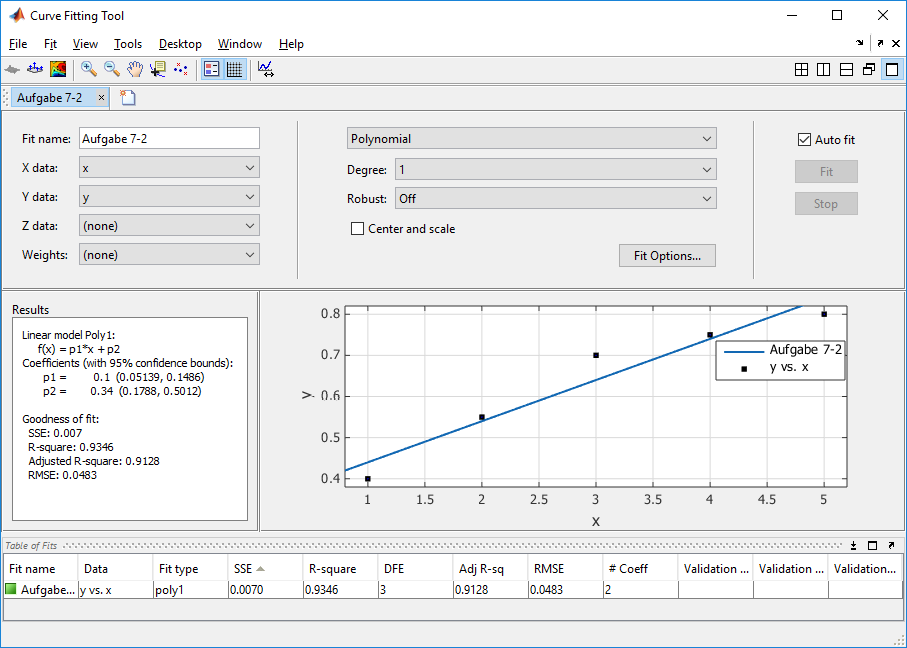
\includegraphics[width=160mm]{02_vorlesung/media/Matlab_CFTool.png}
		\caption{Lösung der Aufgabe mit dem polyfit Befehl von Matlab/Octave. 
		Es wird hier u.~a. der 95\%ige Vertrauensbereich berechnet und
		angezeigt (siehe Mitte links in der Abbildung).}
		\label{fig:MatlabPolyfit}
	\end{center}
\end{figure}

\textbf{Hinweis: Vertrauensbereich} \\
In einer der nächsten Vorlesungen werden wir sehen wie man Vertrauensbereiche 
mit Hilfe der Varianzen bzw. Standardabweichungen berechnet. Dazu benötigt man 
noch die t-Verteilung. Da man hier 5 Messpunkte und 2 Modellparameter hat,
wird die t-Verteilung mit dem Freiheitsgrad 5-2 = 3 benötigt. 
95\%iger Vertrauensbereich für $\hat\theta_1$ mit $t_3 = 3.182$: 
\[
\varepsilon _{\hat{\theta}_1} = t_3 \cdot \hat\sigma_{\theta_1} = \frac{t_3 \cdot s(\hat{\theta}_0 ,
	\hat{\theta}_1 )}{s_X \cdot \sqrt {J
		- 1} } = 0.0486
\]
95\%iger Vertrauensbereich für $\hat\theta_0$ errechnet sich durch:
\[
\varepsilon _{\hat{\theta}_0} = t_3 \cdot \hat\sigma_{\theta_0} = t_3 \cdot s(\hat{\theta}_0 ,\hat{\theta}_1 ) \cdot \sqrt {\frac{1}{J} + \frac{\bar {X}^2}{(J - 1) s_X^2 }} = 0.1612
\]
\textbf{Ergebnis:} \\ 
Der 95\% Vertrauensbereich des Schätzwertes $\hat\theta_1$ ist somit gegeben durch:
\begin{equation}
\hat\theta_1 = 0.1000 \pm 0.0486 \quad \text{bzw.} \quad [0.0514;0.1486]
\end{equation}
Der 95\% Vertrauensbereich des Schätzwertes $\hat\theta_0$ ist somit gegeben durch: 
\begin{equation}
\hat\theta_1 = 0.3400 \pm 0.1612 \quad \text{bzw.} \quad [0.1788;0.5012]
\end{equation}


\begin{comment}
95\%iger Vertrauensbereich für $\hat\theta_1$ mit $t_3 = 3.182$ und 
Standardabweichung von $s_X = 1.5811$
\[
\varepsilon _{\hat{\theta}_1} = \frac{t_3 \cdot s(\hat{\theta}_0 ,
\hat{\theta}_1 )}{s_X \cdot \sqrt {J
- 1} } = 0.0486
\]
95\%iger Vertrauensbereich für $\hat\theta_0$ errechnet sich durch:
\[
\varepsilon _{\hat{\theta}_0} = t_3 \cdot s(\hat{\theta}_0 ,\hat{\theta}_1 ) \cdot \sqrt {\frac{1}{J} + \frac{\bar {X}^2}{(J - 1) s_X^2 }} = 0.1612
\]
\textbf{Ergebnis:} \\ 
Der 95\% Vertrauensbereich des Schätzwertes $\hat\theta_1$ ist somit gegeben durch:
\begin{equation}
\hat\theta_1 = 0.1000 \pm 0.0486 \quad \text{bzw.} \quad [0.0514;0.1486]
\end{equation}
Der 95\% Vertrauensbereich des Schätzwertes $\hat\theta_0$ ist somit gegeben durch: 
\begin{equation}
\hat\theta_1 = 0.3400 \pm 0.1612 \quad \text{bzw.} \quad [0.1788;0.5012]
\end{equation}
\end{comment}


\pagebreak

Für die Unermüdlichen, die lieber in C programmieren, hier die Routine zum Lösen
des linearen Gleichungssystems, haben wir eine Routine zum Lösen von linearen
Gleichungssystemen aus den Numerical Recipes abgedruckt:

B. P. Flannery, W. H. Press, S. A. Teukolsky, W. T. Vetterling. \textsl{Numerical Recipes
in C}. Cambridge University Press, 2.~Auflage (1992-2002)

Wichtig, diese Routine überschreibt den Vektor mit der Inhomogenität des Gleichungssystems
mit der Lösung, also den gewünschten Modellparametern und 
die Matrix \texttt{a} mit den Summen aus den Regressoren mit deren Inversen
\texttt{a}$^{-1}$, die Sie dann für die Kovarianz der Modellparameter brauchen.

\begin{verbatim}
void gaussjordan(double **a, int n, double **b, int m)
/*
* Linear equation solution by Gauss-Jordan elimination, equation (2.1.1) in
* Numerical Recipes.
* a[0..n-1][0..n-1] is the input matrix. b[0..m-1][0..n-1] is input
* containing the m right-hand side vectors.
* For most applications we have m = 1
* On output, a is replaced by its matrix inverse,
* and b is replaced by the corresponding set of solution vectors.
*/
int *indxc,*indxr,*ipiv;
int i,icol,irow,j,k,l,ll;
double big,tmp,pivinv;

// The integer arrays ipiv, indxr, and indxc are
// used for bookkeeping on the pivoting.
indxc = (int*)calloc( n, sizeof(int));
indxr = (int*)calloc( n, sizeof(int));

ipiv = (int*)calloc( n, sizeof(int));

/*	for (j=1;j<=n;j++) ipiv[j]=0;*/
/*	for (j=1;j<=n;j++) ipiv[j]=0;*/
/* calloc initializes to zero:
Allocates a block of memory for an array of num elements,
each of them size bytes long, and initializes all its bits to zero.
*/

/*
* This is the main loop over the columns to be reduced.
*/
for (i=0; i<n; i++) {
big=0.0;

// This is the outer loop of the search for a pivot element.
for (j=0; j<n; j++)
if (ipiv[j] != 1)
for (k=0; k<n; k++) {
if (ipiv[k] == 0) {
if (fabs(a[k][j]) >= big) {
big=fabs(a[k][j]);
irow=j;
icol=k;
}
}
}
++(ipiv[icol]);

/*
* We now have the pivot element, so we interchange rows, if needed,
* to put the pivot element on the diagonal. The columns are not
* physically interchanged, only relabeled:
* indxc[i], the column of the ith pivot element,
*           is the ith column that is reduced, while
* indxr[i] is the row in which that pivot element was originally located.
*          If indxr[i] !=
* indxc[i] there is an implied column interchange.
* With this form of bookkeeping, the solution b-s will end up in the
* correct order, and the inverse matrix will be scrambled by columns.
*/

if (irow != icol) {
for (l=0; l<n; l++) SWAP(a[l][irow],a[l][icol])
for (l=0; l<m; l++) SWAP(b[l][irow],b[l][icol])
}

/*
* We are now ready to divide the pivot row by the
* pivot element, located at irow and icol.
*/

indxr[i]=irow;
indxc[i]=icol;
if (a[icol][icol] == 0.0) printf("gaussj: Singular Matrix\n");
pivinv=1.0/a[icol][icol];
a[icol][icol]=1.0;
for (l=0; l<n; l++) a[l][icol] *= pivinv;
for (l=0; l<m; l++) b[l][icol] *= pivinv;

/*
* Next, we reduce the rows
* except, if (ll != icol), for the pivot one, of course.
*/
for (ll=0; ll<n; ll++)
if (ll != icol) {
tmp=a[icol][ll];
a[icol][ll]=0.0;
for (l=0; l<n; l++) a[l][ll] -= a[l][icol]*tmp;
for (l=0; l<m; l++) b[l][ll] -= b[l][icol]*tmp;
}
}
/*
* This is the end of the main loop over columns of the reduction.
*/

/*
* It only remains to unscramble the solution in view of the column interchanges.
* We do this by interchanging pairs ofcolumns in the reverse order
* that the permutation was built up.
*/
for (l=n-1; l>=0;l--) {
if (indxr[l] != indxc[l])
for (k=0; k<n; k++) SWAP(a[indxr[l]][k],a[indxc[l]][k]);
}
// And we are done.
free(ipiv);
free(indxr);
free(indxc);
}
\end{verbatim}



\section{Hilfe zu den Übungsaufgaben \ref{AufgVorl5} zum Selbststudium}

\textbf{\large Hilfestellung Aufgabe 1}

Ein Gnu-Octave/Matlab Skript für KS-Tests verschiedener Stichproben
kann beispielsweise so aussehen:
\begin{verbatim}
function learn_KS(flagnew)
  N1 = 2000; mu1 = 23; s1 = 3;
  N2 = 450; mu2 = 35; s2 = 5;
  if (flagnew==1)
    x1 = s1*randn(N1,1) + mu1;
    x2 = s2*randn(N2,1) + mu2;
    save 'learn_robust.dat' x1 x2
  else
    load('learn_robust.dat');
  end
  x = [x1; x2];
  KStest(x1, 10);
  KStest(x2, 20);
  KStest(x, 0);
  di = abs(x - mean(x));
  medd = median(di);
  iuse = find( di < medd );
  for itest = 1:4
    KStest(x(iuse), itest);
    di = abs(x(iuse) - mean(x));
    medd = median(di);
    iuse2 = find( di < medd );
    iuse = iuse(iuse2);
  end
end
function KStest(x, iplt)
  alpha = 0.05;
  Ntot = length(x)
  [xsort, isort] = sort(x, 'ascend');
  h = [1:Ntot]'/Ntot;
  xbar = mean(x)
  sbar = std(x)
  g = normcdf( xsort, xbar, sbar);
  K = sqrt(-0.5*log(alpha/2))/sqrt(Ntot);
  figure(3000+iplt);
  plot( xsort, h, 'k-;{\fontsize{14}empirisches Histogramm};', ...
        xsort, g, 'r-;{\fontsize{14}Vert. aus Mittelw./ empir. Var.};');
  xlabel('X', 'fontsize', 14);
  ylabel('Wahrscheinlichkeitsdichte', 'fontsize', 12);
  title(['Stichprobenumfang: ' num2str(Ntot)], 'fontsize', 14);
  grid on;
  legend(gca, 'location', 'northwest');
  set(gca, 'fontsize', 14, 'linewidth', 2);
%
  figure(3100+iplt);
  plot( xsort, abs(g - h), 'b.;{\fontsize{14}abs. Diff.};', ...
        [xsort(1); xsort(Ntot)], [K; K], 'r-;{\fontsize{14}K_{\alpha,J}};');
  xlabel('X', 'fontsize', 14);
  ylabel('abs. Differenz d. Wahrscheinlichkeitsdichte', 'fontsize', 12);
  title(['Stichprobenumfang J = ' num2str(Ntot)], 'fontsize', 14);
  legend(gca, 'location', 'northwest');
  grid on;
  set(gca, 'fontsize', 14, 'linewidth', 2);
end
\end{verbatim}

\textbf{\large Lösung zu Aufgabe 2}

Gegeben seien zwei Stichproben

Stichprobe 1:

\begin{tabular}{|c|c|c|c|c|}
\hline
21 & 33 & 19 & 39 & 7\\
\hline
\end{tabular}

Stichprobe 2:

\begin{tabular}{|c|c|c|c|c|c|c|c|c|}
\hline
53 & 69 & 63 & 47 & 49 & 44 & 47 & 44 & 38\\
\hline
\end{tabular}

\begin{itemize}
\item[a)] Zu jeder der beiden Stichproben die Mittelwerte und Standardabweichungen:

Stichprobe 1: Mittelwert $\bar x_1 = $ (21 + 33 + 19 + 39 + 7)/5 = 23.8,
Standardabweichung $s_1 = $ $\sqrt{((21-23.8)^2 + (33-23.8)^2 + (19-23.8)^2 + (39-23.8)^2 + (7-23.8)^2)/(5-1)}$ $= 12.54$

Stichprobe 2: Mittelwert $\bar x_2 = 50.44$, Standardabweichung $s_2 = 9.83$

\item[b)] Nullhypothese $H_0$: $\mu_1 = \mu_2$
$$
T \; = \; \frac{\bar x_1 \, - \, \bar x_2}{\sqrt{\bar s_1^2 + \bar s_2^2}}
$$
Varianzen der Mittelwerte:
$$
\bar s_1^2 = \frac{s_1^2}{5} = \frac{(12.54)^2}{5} = 31.44
\qquad
\bar s_2^2 = \frac{s_2^2}{9} = \frac{(9.83)^2}{9} = 10.73
$$
damit
$$
T \; = \; \frac{23.8 \, - \, 50.44}{\sqrt{31.44 + 10.73}} = -5.84
$$
t-Quantil für Signifikanzniveau $\alpha = 0.05$ für zweiseitige Verteilung:
$t_{1-\alpha/2,\nu} = t_{0.975,5+9-2} = 2.18$

Ergebnis: $|T| = 5.84 > 2.18$ also Nullhypothese ablehnen

\item[c)] Nullhypothese $H_0$: $s_2^2 = \sigma_0^2$ mit $\sigma_0 = 6$
$$
T \; = \; \nu \, \left( \frac{s_2}{\sigma_0} \right)^2
$$
mit $\nu = 9-1$ für Stichprobe 2
$$
T \; = \; 8 \, \left( \frac{9.83}{6} \right)^2 = 21.45
$$
$\chi^2$-Quantile für Signifikanzniveau $\alpha = 0.05$ sind
$\chi^2_{\alpha/2,\nu} = \chi^2_{0.025,8} = 2.180$ und
$\chi^2_{1-\alpha/2,\nu} = \chi^2_{0.975,8} = 17.535$

Gilt $\chi^2_{\alpha/2,\nu} < T < \chi^2_{1-\alpha/2,\nu}$?

Ergebnis: $2.180 < 21.45$ aber $21.45$ ist nicht kleiner als $17.535$, also $H_0$ ablehnen

\item[c)] Nullhypothese $H_0$: $s_2^2 = \sigma_0^2$ mit $\sigma_0 = 9$
$$
T \; = \; 8 \, \left( \frac{9.83}{9} \right)^2 = 9.53
$$
Ergebnis:
T liegt zwischen den Quantilen $2.180 < 9.53 < 17.535$, also $H_0$ annehmen
\end{itemize}





\begin{thebibliography}{------}
    \bibitem[Fla02]{Fla02} B. P. Flannery, W. H. Press, S. A. Teukolsky, and W. T. Vetterling. Numerical Recipes in C. Cambridge University Press, 2. edition (1992-2002)
%    \bibitem[Els07]{Els07} C. Elster: Calculation of unceratinty
%	in the presence of prior knowledge, Metrologia 44, 111-116, (2007)
%    \bibitem[Cox06]{Cox06} M.G. Cox, B.R.L. Siebert:The use of
%    a Monte Carlo method for evaluating ..., Metrologie 43, S178-88,
%    (2006)
%    \bibitem[GUMS1]{GUMS1} 
%    JCGM 101:2008; Evaluation of measurement data — Supplement 1 to the 
%    “Guide to the expression of uncertainty in measurement” — 
%    Propagation of distributions using a Monte Carlo method (2008); \newline 
%    https://www.bipm.org/utils/common/documents/jcgm/JCGM\_101\_2008\_E.pdf
%    \bibitem[Wue08]{Wue08} Gerd Wübbeler, Michael Krystek and Clemens Elster: % % %    Evaluation of measurement uncertainty
%    and its numerical calculation by a Monte Carlo method
%    Meas. Sci. Technol. 19 (2008) 084009 (4pp)
%   doi:10.1088/0957-0233/19/8/084009
\end{thebibliography}

\end{document}


